\documentclass[twoside]{book}

% Packages required by doxygen
\usepackage{calc}
\usepackage{doxygen}
\usepackage{graphicx}
\usepackage[utf8]{inputenc}
\usepackage{makeidx}
\usepackage{multicol}
\usepackage{multirow}
\usepackage{fixltx2e}
\PassOptionsToPackage{warn}{textcomp}
\usepackage{textcomp}
\usepackage[nointegrals]{wasysym}
\usepackage[table]{xcolor}

% Font selection
\usepackage[T1]{fontenc}
\usepackage{mathptmx}
\usepackage[scaled=.90]{helvet}
\usepackage{courier}
\usepackage{amssymb}
\usepackage{sectsty}
\renewcommand{\familydefault}{\sfdefault}
\allsectionsfont{%
  \fontseries{bc}\selectfont%
  \color{darkgray}%
}
\renewcommand{\DoxyLabelFont}{%
  \fontseries{bc}\selectfont%
  \color{darkgray}%
}
\newcommand{\+}{\discretionary{\mbox{\scriptsize$\hookleftarrow$}}{}{}}

% Page & text layout
\usepackage{geometry}
\geometry{%
  a4paper,%
  top=2.5cm,%
  bottom=2.5cm,%
  left=2.5cm,%
  right=2.5cm%
}
\tolerance=750
\hfuzz=15pt
\hbadness=750
\setlength{\emergencystretch}{15pt}
\setlength{\parindent}{0cm}
\setlength{\parskip}{0.2cm}
\makeatletter
\renewcommand{\paragraph}{%
  \@startsection{paragraph}{4}{0ex}{-1.0ex}{1.0ex}{%
    \normalfont\normalsize\bfseries\SS@parafont%
  }%
}
\renewcommand{\subparagraph}{%
  \@startsection{subparagraph}{5}{0ex}{-1.0ex}{1.0ex}{%
    \normalfont\normalsize\bfseries\SS@subparafont%
  }%
}
\makeatother

% Headers & footers
\usepackage{fancyhdr}
\pagestyle{fancyplain}
\fancyhead[LE]{\fancyplain{}{\bfseries\thepage}}
\fancyhead[CE]{\fancyplain{}{}}
\fancyhead[RE]{\fancyplain{}{\bfseries\leftmark}}
\fancyhead[LO]{\fancyplain{}{\bfseries\rightmark}}
\fancyhead[CO]{\fancyplain{}{}}
\fancyhead[RO]{\fancyplain{}{\bfseries\thepage}}
\fancyfoot[LE]{\fancyplain{}{}}
\fancyfoot[CE]{\fancyplain{}{}}
\fancyfoot[RE]{\fancyplain{}{\bfseries\scriptsize Generated on Wed Oct 1 2014 14\+:16\+:05 for Exact Stochastic Simulation Software by Doxygen }}
\fancyfoot[LO]{\fancyplain{}{\bfseries\scriptsize Generated on Wed Oct 1 2014 14\+:16\+:05 for Exact Stochastic Simulation Software by Doxygen }}
\fancyfoot[CO]{\fancyplain{}{}}
\fancyfoot[RO]{\fancyplain{}{}}
\renewcommand{\footrulewidth}{0.4pt}
\renewcommand{\chaptermark}[1]{%
  \markboth{#1}{}%
}
\renewcommand{\sectionmark}[1]{%
  \markright{\thesection\ #1}%
}

% Indices & bibliography
\usepackage{natbib}
\usepackage[titles]{tocloft}
\setcounter{tocdepth}{3}
\setcounter{secnumdepth}{5}
\makeindex

% Hyperlinks (required, but should be loaded last)
\usepackage{ifpdf}
\ifpdf
  \usepackage[pdftex,pagebackref=true]{hyperref}
\else
  \usepackage[ps2pdf,pagebackref=true]{hyperref}
\fi
\hypersetup{%
  colorlinks=true,%
  linkcolor=blue,%
  citecolor=blue,%
  unicode%
}

% Custom commands
\newcommand{\clearemptydoublepage}{%
  \newpage{\pagestyle{empty}\cleardoublepage}%
}


%===== C O N T E N T S =====

\begin{document}

% Titlepage & ToC
\hypersetup{pageanchor=false,
             bookmarks=true,
             bookmarksnumbered=true,
             pdfencoding=unicode
            }
\pagenumbering{roman}
\begin{titlepage}
\vspace*{7cm}
\begin{center}%
{\Large Exact Stochastic Simulation Software }\\
\vspace*{1cm}
{\large Generated by Doxygen 1.8.7}\\
\vspace*{0.5cm}
{\small Wed Oct 1 2014 14:16:05}\\
\end{center}
\end{titlepage}
\clearemptydoublepage
\tableofcontents
\clearemptydoublepage
\pagenumbering{arabic}
\hypersetup{pageanchor=true}

%--- Begin generated contents ---
\chapter{Documentation}
\label{index}\hypertarget{index}{}\input{index}
\chapter{Namespace Documentation}
\hypertarget{namespacenw}{\section{nw Namespace Reference}
\label{namespacenw}\index{nw@{nw}}
}
\subsection*{Classes}
\begin{DoxyCompactItemize}
\item 
class \hyperlink{classnw_1_1___event}{\+\_\+\+Event}
\begin{DoxyCompactList}\small\item\em Abstract base class for system state transitions (events). \end{DoxyCompactList}\item 
class \hyperlink{classnw_1_1___input}{\+\_\+\+Input}
\begin{DoxyCompactList}\small\item\em Abstract base class for input procedures. \end{DoxyCompactList}\item 
class \hyperlink{classnw_1_1___random}{\+\_\+\+Random}
\begin{DoxyCompactList}\small\item\em abstract base class to define an interface for Random Generators \end{DoxyCompactList}\item 
class \hyperlink{classnw_1_1___species}{\+\_\+\+Species}
\begin{DoxyCompactList}\small\item\em Abstract base class for the molecular species of a system. \end{DoxyCompactList}\item 
class \hyperlink{classnw_1_1___system}{\+\_\+\+System}
\begin{DoxyCompactList}\small\item\em Abstract base class for the implementation of simulation algorithms. \end{DoxyCompactList}\item 
class \hyperlink{classnw_1_1___voxel}{\+\_\+\+Voxel}
\begin{DoxyCompactList}\small\item\em Abstract base class for voxel (discrete building blocks of the simulation volume) \end{DoxyCompactList}\item 
class \hyperlink{classnw_1_1_border___vxl}{Border\+\_\+\+Vxl}
\begin{DoxyCompactList}\small\item\em Specialized \hyperlink{classnw_1_1___voxel}{\+\_\+\+Voxel} that can be used to define a system with equilibrium as boundary condition. \end{DoxyCompactList}\item 
class \hyperlink{classnw_1_1_channel___spc}{Channel\+\_\+\+Spc}
\begin{DoxyCompactList}\small\item\em Realization of channel proteins comprised of a fixed number of subunits that open whenever a predefined number of those subunits are in an active state. \end{DoxyCompactList}\item 
class \hyperlink{classnw_1_1_ch_flux___rct___evt}{Ch\+Flux\+\_\+\+Rct\+\_\+\+Evt}
\begin{DoxyCompactList}\small\item\em Channel flux reaction event. \end{DoxyCompactList}\item 
class \hyperlink{classnw_1_1_diffusion___evt}{Diffusion\+\_\+\+Evt}
\begin{DoxyCompactList}\small\item\em Realization of diffusion between two voxels. \end{DoxyCompactList}\item 
class \hyperlink{classnw_1_1_gillespie___sys}{Gillespie\+\_\+\+Sys}
\begin{DoxyCompactList}\small\item\em Coordinates the stochastic simulation algorithm. \end{DoxyCompactList}\item 
class \hyperlink{classnw_1_1_reaction___evt}{Reaction\+\_\+\+Evt}
\begin{DoxyCompactList}\small\item\em Implementation of the reaction of one ore two molecules. \end{DoxyCompactList}\item 
class \hyperlink{classnw_1_1_standard___ipt}{Standard\+\_\+\+Ipt}
\begin{DoxyCompactList}\small\item\em Input class that parses a .xml files and generates a \hyperlink{classnw_1_1_gillespie___sys}{Gillespie\+\_\+\+Sys}. \end{DoxyCompactList}\item 
class \hyperlink{classnw_1_1_standard___spc}{Standard\+\_\+\+Spc}
\begin{DoxyCompactList}\small\item\em Basic implementation of a standard moecular species. \end{DoxyCompactList}\item 
class \hyperlink{classnw_1_1_standard___vxl}{Standard\+\_\+\+Vxl}
\begin{DoxyCompactList}\small\item\em Standard voxel implementation. \end{DoxyCompactList}\item 
class \hyperlink{classnw_1_1_sub_unit_switch___rct___evt}{Sub\+Unit\+Switch\+\_\+\+Rct\+\_\+\+Evt}
\begin{DoxyCompactList}\small\item\em Subunit switch reaction event. \end{DoxyCompactList}\item 
class \hyperlink{classnw_1_1_uni___rnd}{Uni\+\_\+\+Rnd}
\begin{DoxyCompactList}\small\item\em \char`\"{}\+Minimal\char`\"{} random number generator of Park and Miller \end{DoxyCompactList}\end{DoxyCompactItemize}
\subsection*{Typedefs}
\begin{DoxyCompactItemize}
\item 
typedef vector$<$ \hyperlink{classnw_1_1___voxel}{\+\_\+\+Voxel} $\ast$ $>$ \hyperlink{namespacenw_ad7146b8b5a9de9be416847f41135722c}{Voxel\+Vector}
\begin{DoxyCompactList}\small\item\em typedefs of Vector related structures \end{DoxyCompactList}\item 
typedef Voxel\+Vector\+::iterator \hyperlink{namespacenw_a79f35b5a82b764c7144ecf3074e926c0}{Voxel\+Iterator}
\begin{DoxyCompactList}\small\item\em typedefs of a \hyperlink{classnw_1_1___voxel}{\+\_\+\+Voxel} vector iterator \end{DoxyCompactList}\item 
typedef vector$<$ \hyperlink{classnw_1_1___event}{\+\_\+\+Event} $\ast$ $>$ \hyperlink{namespacenw_a0d9ea27d7802637354c7892806eac1fc}{Event\+Vector}
\begin{DoxyCompactList}\small\item\em typedefs of a \hyperlink{classnw_1_1___event}{\+\_\+\+Event} reference vector \end{DoxyCompactList}\item 
typedef Event\+Vector\+::iterator \hyperlink{namespacenw_a543a4f72e609ca94582c1c7c10303e0b}{Event\+Iterator}
\begin{DoxyCompactList}\small\item\em typedefs of a \hyperlink{classnw_1_1___event}{\+\_\+\+Event} vector iterator \end{DoxyCompactList}\item 
typedef vector$<$ \hyperlink{classnw_1_1___species}{\+\_\+\+Species} $\ast$ $>$ \hyperlink{namespacenw_a68aa8285591d78ebfc793c531bd43a23}{Species\+Vector}
\begin{DoxyCompactList}\small\item\em typedefs of Species related structures \end{DoxyCompactList}\item 
typedef Species\+Vector\+::iterator \hyperlink{namespacenw_a28941aaaa0562445c168a620b63547d2}{Species\+Iterator}
\end{DoxyCompactItemize}
\subsection*{Variables}
\begin{DoxyCompactItemize}
\item 
static const double \hyperlink{namespacenw_ad890cfa7dd9eaf8d5b6754723e516c4a}{N\+\_\+\+A\+V\+O} = 6.\+022e23
\item 
static const string \hyperlink{namespacenw_a7d9622d3fd42f8d91bb8b8a79688518d}{N\+E\+G\+A\+T\+I\+V\+E\+T\+A\+U\+M\+S\+G} = \char`\"{}N\+E\+G\+A\+T\+I\+V\+E T\+A\+U E\+R\+R\+O\+R L\+A\+S\+T E\+V\+E\+N\+T \char`\"{}
\begin{DoxyCompactList}\small\item\em Error message that is thrown, whenever the smallest tau value becomes negative. \end{DoxyCompactList}\end{DoxyCompactItemize}


\subsection{Typedef Documentation}
\hypertarget{namespacenw_a543a4f72e609ca94582c1c7c10303e0b}{\index{nw@{nw}!Event\+Iterator@{Event\+Iterator}}
\index{Event\+Iterator@{Event\+Iterator}!nw@{nw}}
\subsubsection[{Event\+Iterator}]{\setlength{\rightskip}{0pt plus 5cm}typedef Event\+Vector\+::iterator {\bf nw\+::\+Event\+Iterator}}}\label{namespacenw_a543a4f72e609ca94582c1c7c10303e0b}


typedefs of a \hyperlink{classnw_1_1___event}{\+\_\+\+Event} vector iterator 

\hypertarget{namespacenw_a0d9ea27d7802637354c7892806eac1fc}{\index{nw@{nw}!Event\+Vector@{Event\+Vector}}
\index{Event\+Vector@{Event\+Vector}!nw@{nw}}
\subsubsection[{Event\+Vector}]{\setlength{\rightskip}{0pt plus 5cm}typedef vector$<${\bf \+\_\+\+Event}$\ast$$>$ {\bf nw\+::\+Event\+Vector}}}\label{namespacenw_a0d9ea27d7802637354c7892806eac1fc}


typedefs of a \hyperlink{classnw_1_1___event}{\+\_\+\+Event} reference vector 

\hypertarget{namespacenw_a28941aaaa0562445c168a620b63547d2}{\index{nw@{nw}!Species\+Iterator@{Species\+Iterator}}
\index{Species\+Iterator@{Species\+Iterator}!nw@{nw}}
\subsubsection[{Species\+Iterator}]{\setlength{\rightskip}{0pt plus 5cm}typedef Species\+Vector\+::iterator {\bf nw\+::\+Species\+Iterator}}}\label{namespacenw_a28941aaaa0562445c168a620b63547d2}
\hypertarget{namespacenw_a68aa8285591d78ebfc793c531bd43a23}{\index{nw@{nw}!Species\+Vector@{Species\+Vector}}
\index{Species\+Vector@{Species\+Vector}!nw@{nw}}
\subsubsection[{Species\+Vector}]{\setlength{\rightskip}{0pt plus 5cm}typedef vector$<${\bf \+\_\+\+Species}$\ast$$>$ {\bf nw\+::\+Species\+Vector}}}\label{namespacenw_a68aa8285591d78ebfc793c531bd43a23}


typedefs of Species related structures 

\hypertarget{namespacenw_a79f35b5a82b764c7144ecf3074e926c0}{\index{nw@{nw}!Voxel\+Iterator@{Voxel\+Iterator}}
\index{Voxel\+Iterator@{Voxel\+Iterator}!nw@{nw}}
\subsubsection[{Voxel\+Iterator}]{\setlength{\rightskip}{0pt plus 5cm}typedef Voxel\+Vector\+::iterator {\bf nw\+::\+Voxel\+Iterator}}}\label{namespacenw_a79f35b5a82b764c7144ecf3074e926c0}


typedefs of a \hyperlink{classnw_1_1___voxel}{\+\_\+\+Voxel} vector iterator 

\hypertarget{namespacenw_ad7146b8b5a9de9be416847f41135722c}{\index{nw@{nw}!Voxel\+Vector@{Voxel\+Vector}}
\index{Voxel\+Vector@{Voxel\+Vector}!nw@{nw}}
\subsubsection[{Voxel\+Vector}]{\setlength{\rightskip}{0pt plus 5cm}typedef vector$<$ {\bf \+\_\+\+Voxel} $\ast$ $>$ {\bf nw\+::\+Voxel\+Vector}}}\label{namespacenw_ad7146b8b5a9de9be416847f41135722c}


typedefs of Vector related structures 

typedefs of a \hyperlink{classnw_1_1___voxel}{\+\_\+\+Voxel} reference vector 

\subsection{Variable Documentation}
\hypertarget{namespacenw_ad890cfa7dd9eaf8d5b6754723e516c4a}{\index{nw@{nw}!N\+\_\+\+A\+V\+O@{N\+\_\+\+A\+V\+O}}
\index{N\+\_\+\+A\+V\+O@{N\+\_\+\+A\+V\+O}!nw@{nw}}
\subsubsection[{N\+\_\+\+A\+V\+O}]{\setlength{\rightskip}{0pt plus 5cm}const double nw\+::\+N\+\_\+\+A\+V\+O = 6.\+022e23\hspace{0.3cm}{\ttfamily [static]}}}\label{namespacenw_ad890cfa7dd9eaf8d5b6754723e516c4a}
Definition of Avogadro's constant \hypertarget{namespacenw_a7d9622d3fd42f8d91bb8b8a79688518d}{\index{nw@{nw}!N\+E\+G\+A\+T\+I\+V\+E\+T\+A\+U\+M\+S\+G@{N\+E\+G\+A\+T\+I\+V\+E\+T\+A\+U\+M\+S\+G}}
\index{N\+E\+G\+A\+T\+I\+V\+E\+T\+A\+U\+M\+S\+G@{N\+E\+G\+A\+T\+I\+V\+E\+T\+A\+U\+M\+S\+G}!nw@{nw}}
\subsubsection[{N\+E\+G\+A\+T\+I\+V\+E\+T\+A\+U\+M\+S\+G}]{\setlength{\rightskip}{0pt plus 5cm}const string nw\+::\+N\+E\+G\+A\+T\+I\+V\+E\+T\+A\+U\+M\+S\+G = \char`\"{}N\+E\+G\+A\+T\+I\+V\+E T\+A\+U E\+R\+R\+O\+R L\+A\+S\+T E\+V\+E\+N\+T \char`\"{}\hspace{0.3cm}{\ttfamily [static]}}}\label{namespacenw_a7d9622d3fd42f8d91bb8b8a79688518d}


Error message that is thrown, whenever the smallest tau value becomes negative. 


\chapter{Class Documentation}
\hypertarget{classnw_1_1___event}{\section{nw\+:\+:\+\_\+\+Event Class Reference}
\label{classnw_1_1___event}\index{nw\+::\+\_\+\+Event@{nw\+::\+\_\+\+Event}}
}


Abstract base class for system state transitions (events).  




{\ttfamily \#include $<$\+\_\+\+Event.\+h$>$}

Inheritance diagram for nw\+:\+:\+\_\+\+Event\+:\begin{figure}[H]
\begin{center}
\leavevmode
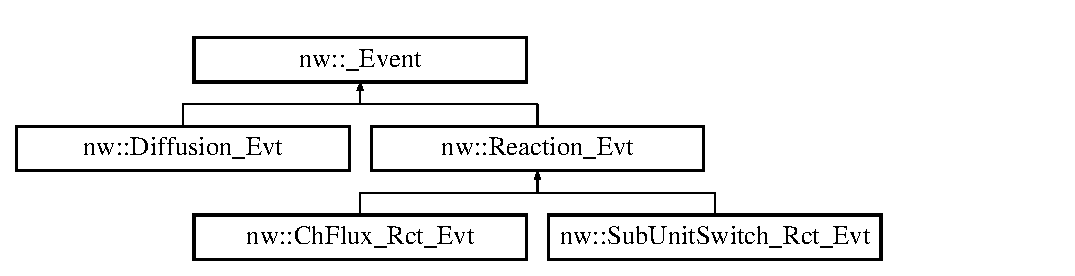
\includegraphics[height=3.000000cm]{d8/d98/classnw_1_1___event}
\end{center}
\end{figure}
\subsection*{Classes}
\begin{DoxyCompactItemize}
\item 
struct \hyperlink{structnw_1_1___event_1_1tv__struct}{tv\+\_\+struct}
\begin{DoxyCompactList}\small\item\em tau-\/voxel-\/structure (\hyperlink{structnw_1_1___event_1_1tv__struct}{tv\+\_\+struct}) is a structure that associates a tau value with a \hyperlink{classnw_1_1___voxel}{\+\_\+\+Voxel}. \end{DoxyCompactList}\end{DoxyCompactItemize}
\subsection*{Public Member Functions}
\begin{DoxyCompactItemize}
\item 
\hyperlink{classnw_1_1___event_a5efb757db20b083de6da605ea4b2bbae}{\+\_\+\+Event} (long \hyperlink{classnw_1_1___event_a8f7ce287f596266dd763ec7db2f74090}{id}, string \hyperlink{classnw_1_1___event_ab4f50a54039cd4957bdca55049178562}{name}, double \hyperlink{classnw_1_1___event_afca0ae816e9834add07db8e9a6618faa}{k}, \hyperlink{namespacenw_ad7146b8b5a9de9be416847f41135722c}{Voxel\+Vector} vvc, \hyperlink{classnw_1_1_uni___rnd}{Uni\+\_\+\+Rnd} $\ast$\hyperlink{classnw_1_1___event_af92482aeea55562560573ecccd5ab108}{rg})
\begin{DoxyCompactList}\small\item\em Constructor. \end{DoxyCompactList}\item 
virtual \hyperlink{classnw_1_1___event_aede7a9b059e398c72320ad6d27ad6b2d}{$\sim$\+\_\+\+Event} ()
\begin{DoxyCompactList}\small\item\em Destructor. \end{DoxyCompactList}\item 
virtual double \hyperlink{classnw_1_1___event_a882115f8652c881bc8ed43f1050ccba3}{update} (double last\+\_\+tau)=0
\begin{DoxyCompactList}\small\item\em Updates the event. \end{DoxyCompactList}\item 
virtual void \hyperlink{classnw_1_1___event_aa022418fb765582a053ac75cbc3436d6}{execute} ()=0
\begin{DoxyCompactList}\small\item\em Event execution function. \end{DoxyCompactList}\item 
virtual void \hyperlink{classnw_1_1___event_ae2c608ee2508058d6f318ca2ca8f4317}{init} ()=0
\begin{DoxyCompactList}\small\item\em Event initialization. \end{DoxyCompactList}\item 
virtual double \hyperlink{classnw_1_1___event_a75945699f539cefab36eb6693a389918}{get\+\_\+a} ()=0
\begin{DoxyCompactList}\small\item\em returns current \hyperlink{classnw_1_1___event}{\+\_\+\+Event} propensity a. \end{DoxyCompactList}\item 
void \hyperlink{classnw_1_1___event_afae58637d427d9fa023850a1f8342912}{add\+\_\+dep\+\_\+list} (\hyperlink{classnw_1_1___event}{\+\_\+\+Event} $\ast$e)
\begin{DoxyCompactList}\small\item\em Adds an \hyperlink{classnw_1_1___event}{\+\_\+\+Event} pointer to the dependency list. \end{DoxyCompactList}\item 
void \hyperlink{classnw_1_1___event_a05f533e8b22bece51864a24d1f4d8534}{set\+\_\+flag} (bool b)
\begin{DoxyCompactList}\small\item\em set the dirty flag. \end{DoxyCompactList}\item 
string \hyperlink{classnw_1_1___event_a982b9a043c4bcdd562b29cbba428760f}{get\+\_\+name} ()
\item 
long \hyperlink{classnw_1_1___event_abc5fa1db0c336b4d464f94274a015cf4}{get\+\_\+id} ()
\item 
double \hyperlink{classnw_1_1___event_ae58559a4aa257c900e3ff2e09bc0410b}{get\+\_\+tau} ()
\item 
vector$<$ long $>$ \hyperlink{classnw_1_1___event_a9b32388aa5263ab4ccd16c964c7a4a9b}{get\+\_\+sc\+\_\+vec} ()
\item 
vector$<$ \hyperlink{classnw_1_1___event}{\+\_\+\+Event} $\ast$ $>$ \hyperlink{classnw_1_1___event_a63d2e7f276e03337196eee24c0d43efc}{get\+\_\+dep\+\_\+list} ()
\end{DoxyCompactItemize}
\subsection*{Protected Attributes}
\begin{DoxyCompactItemize}
\item 
long \hyperlink{classnw_1_1___event_a8f7ce287f596266dd763ec7db2f74090}{id}
\begin{DoxyCompactList}\small\item\em I\+D. \end{DoxyCompactList}\item 
string \hyperlink{classnw_1_1___event_ab4f50a54039cd4957bdca55049178562}{name}
\begin{DoxyCompactList}\small\item\em Name. \end{DoxyCompactList}\item 
double \hyperlink{classnw_1_1___event_afca0ae816e9834add07db8e9a6618faa}{k}
\begin{DoxyCompactList}\small\item\em Rate constant. \end{DoxyCompactList}\item 
vector$<$ long $>$ \hyperlink{classnw_1_1___event_a560c8b6f9954a43f5d5f80204473b64d}{sc\+\_\+vec}
\begin{DoxyCompactList}\small\item\em State change vector. Defines an event in terms of a vector, representing the molecular change for each existing \hyperlink{classnw_1_1___species}{\+\_\+\+Species}. \end{DoxyCompactList}\item 
vector$<$ \hyperlink{structnw_1_1___event_1_1tv__struct}{tv\+\_\+struct} $>$ \hyperlink{classnw_1_1___event_a6351b58d94923ed58e0b2cf6c9445d2e}{tv\+\_\+vec}
\begin{DoxyCompactList}\small\item\em Tau voxel vector. Container for tv\+\_\+structs, each representing a \hyperlink{classnw_1_1___voxel}{\+\_\+\+Voxel} where this \hyperlink{classnw_1_1___event}{\+\_\+\+Event} can occur. \end{DoxyCompactList}\item 
\hyperlink{classnw_1_1_uni___rnd}{Uni\+\_\+\+Rnd} $\ast$ \hyperlink{classnw_1_1___event_af92482aeea55562560573ecccd5ab108}{rg}
\begin{DoxyCompactList}\small\item\em Uniform random number generator. \end{DoxyCompactList}\item 
long \hyperlink{classnw_1_1___event_a7864559e204c087306e3becb5b81fb26}{next\+Voxel}
\begin{DoxyCompactList}\small\item\em Index of next \hyperlink{classnw_1_1___voxel}{\+\_\+\+Voxel} to be executed. \end{DoxyCompactList}\item 
double \hyperlink{classnw_1_1___event_a29c77fb164e745cdb5c5fda4f191cd37}{c}
\begin{DoxyCompactList}\small\item\em Adapted \hyperlink{classnw_1_1___event}{\+\_\+\+Event} rate constant. Based on the type of \hyperlink{classnw_1_1___event}{\+\_\+\+Event} {\ttfamily c} is depends on \hyperlink{classnw_1_1___voxel}{\+\_\+\+Voxel} volume (bimoleuclar reactions) or \hyperlink{classnw_1_1___voxel}{\+\_\+\+Voxel} box length (diffusion) \end{DoxyCompactList}\item 
bool \hyperlink{classnw_1_1___event_aaa705b35c06c0cb2e0a4f3daa9ee8037}{dirty\+\_\+flag}
\begin{DoxyCompactList}\small\item\em indicates wheather or not the tau value has to be recalculated ({\ttfamily T\+R\+U\+E}) or adapted to the absolute time scale ({\ttfamily F\+A\+L\+S\+E}) \end{DoxyCompactList}\item 
vector$<$ \hyperlink{classnw_1_1___event}{\+\_\+\+Event} $\ast$ $>$ \hyperlink{classnw_1_1___event_a3f87b2dff69d07977f0a5e10936f38f6}{dep\+\_\+list}
\begin{DoxyCompactList}\small\item\em Dependency vector that stores references to \+\_\+\+Events that depend on this \hyperlink{classnw_1_1___event}{\+\_\+\+Event}. \end{DoxyCompactList}\end{DoxyCompactItemize}


\subsection{Detailed Description}
Abstract base class for system state transitions (events). 

A system state transition is called event and is defined by a propensity function, a state change vector and a dependency list. Propensity functions are derived from rate constants that result either from experimental observations and/or fundamental physical laws. A state change vector represent the stoichiometry of an event and represents the numerical changes in molecular populations caused by the respective event. The dependency list is an implementation of a dependency graph that defines how events influence each other. This data structure is crucial to implement Gibbson and Bruck's optimized update procedure. 

\subsection{Constructor \& Destructor Documentation}
\hypertarget{classnw_1_1___event_a5efb757db20b083de6da605ea4b2bbae}{\index{nw\+::\+\_\+\+Event@{nw\+::\+\_\+\+Event}!\+\_\+\+Event@{\+\_\+\+Event}}
\index{\+\_\+\+Event@{\+\_\+\+Event}!nw\+::\+\_\+\+Event@{nw\+::\+\_\+\+Event}}
\subsubsection[{\+\_\+\+Event}]{\setlength{\rightskip}{0pt plus 5cm}nw\+::\+\_\+\+Event\+::\+\_\+\+Event (
\begin{DoxyParamCaption}
\item[{long}]{id, }
\item[{string}]{name, }
\item[{double}]{k, }
\item[{{\bf Voxel\+Vector}}]{vvc, }
\item[{{\bf Uni\+\_\+\+Rnd} $\ast$}]{rg}
\end{DoxyParamCaption}
)\hspace{0.3cm}{\ttfamily [inline]}}}\label{classnw_1_1___event_a5efb757db20b083de6da605ea4b2bbae}


Constructor. 


\begin{DoxyParams}{Parameters}
{\em id} & Event I\+D \\
\hline
{\em name} & Event name \\
\hline
{\em k} & Rate constant \\
\hline
{\em vvc} & Voxel vector containing all \+\_\+\+Voxels where this \hyperlink{classnw_1_1___event}{\+\_\+\+Event} can occur. \\
\hline
{\em rg} & Random generator that produces uniform distributed random numbers \\
\hline
\end{DoxyParams}

\begin{DoxyCode}
35                                                                         :
36         \hyperlink{classnw_1_1___event_a8f7ce287f596266dd763ec7db2f74090}{id}(\textcolor{keywordtype}{id}),
37         \hyperlink{classnw_1_1___event_ab4f50a54039cd4957bdca55049178562}{name}(\hyperlink{classnw_1_1___event_ab4f50a54039cd4957bdca55049178562}{name}),
38         \hyperlink{classnw_1_1___event_afca0ae816e9834add07db8e9a6618faa}{k}(\hyperlink{classnw_1_1___event_afca0ae816e9834add07db8e9a6618faa}{k}),
39         \hyperlink{classnw_1_1___event_af92482aeea55562560573ecccd5ab108}{rg}(\hyperlink{classnw_1_1___event_af92482aeea55562560573ecccd5ab108}{rg}),
40         \hyperlink{classnw_1_1___event_aaa705b35c06c0cb2e0a4f3daa9ee8037}{dirty\_flag}(\textcolor{keyword}{true})\{
41 
42 \textcolor{comment}{//      add self-reference to dependency list.}
43         this->\hyperlink{classnw_1_1___event_a3f87b2dff69d07977f0a5e10936f38f6}{dep\_list}.push\_back(\textcolor{keyword}{this});
44 \textcolor{comment}{//      check if all voxel in the assigned voxel vector have the same size}
45         \textcolor{keywordflow}{for} (\textcolor{keywordtype}{size\_t} i = 0; i < \hyperlink{classnw_1_1___event_a6351b58d94923ed58e0b2cf6c9445d2e}{tv\_vec}.size(); i++)\{
46             \textcolor{keywordflow}{if}(vvc[i]->get\_volume() != vvc[0]->get\_volume())\{
47                 cout << \textcolor{stringliteral}{"ERROR: Voxel sizes in Event: "} << this->\hyperlink{classnw_1_1___event_ab4f50a54039cd4957bdca55049178562}{name} << \textcolor{stringliteral}{" differ in size. "}
48                         \textcolor{stringliteral}{"You either have to create another Event or resize the voxel to one size"}
49                         << std::endl;
50                 \textcolor{keywordflow}{break};
51             \}
52         \}
53 
54 \textcolor{comment}{//      create the tau voxel structure container that assigns a tau value to each \_Voxel}
55 \textcolor{comment}{//      in the \_Voxel vector}
56         \hyperlink{classnw_1_1___event_a6351b58d94923ed58e0b2cf6c9445d2e}{tv\_vec}.resize(vvc.size());
57         \textcolor{keywordflow}{for}(\textcolor{keywordtype}{size\_t} i = 0; i < \hyperlink{classnw_1_1___event_a6351b58d94923ed58e0b2cf6c9445d2e}{tv\_vec}.size(); i++)\{
58             \hyperlink{classnw_1_1___event_a6351b58d94923ed58e0b2cf6c9445d2e}{tv\_vec}[i].v = vvc[i];
59             \hyperlink{classnw_1_1___event_a6351b58d94923ed58e0b2cf6c9445d2e}{tv\_vec}[i].t = 0.0;
60         \}
61     \}
\end{DoxyCode}
\hypertarget{classnw_1_1___event_aede7a9b059e398c72320ad6d27ad6b2d}{\index{nw\+::\+\_\+\+Event@{nw\+::\+\_\+\+Event}!````~\+\_\+\+Event@{$\sim$\+\_\+\+Event}}
\index{````~\+\_\+\+Event@{$\sim$\+\_\+\+Event}!nw\+::\+\_\+\+Event@{nw\+::\+\_\+\+Event}}
\subsubsection[{$\sim$\+\_\+\+Event}]{\setlength{\rightskip}{0pt plus 5cm}virtual nw\+::\+\_\+\+Event\+::$\sim$\+\_\+\+Event (
\begin{DoxyParamCaption}
{}
\end{DoxyParamCaption}
)\hspace{0.3cm}{\ttfamily [inline]}, {\ttfamily [virtual]}}}\label{classnw_1_1___event_aede7a9b059e398c72320ad6d27ad6b2d}


Destructor. 


\begin{DoxyCode}
63 \{\};
\end{DoxyCode}


\subsection{Member Function Documentation}
\hypertarget{classnw_1_1___event_afae58637d427d9fa023850a1f8342912}{\index{nw\+::\+\_\+\+Event@{nw\+::\+\_\+\+Event}!add\+\_\+dep\+\_\+list@{add\+\_\+dep\+\_\+list}}
\index{add\+\_\+dep\+\_\+list@{add\+\_\+dep\+\_\+list}!nw\+::\+\_\+\+Event@{nw\+::\+\_\+\+Event}}
\subsubsection[{add\+\_\+dep\+\_\+list}]{\setlength{\rightskip}{0pt plus 5cm}void nw\+::\+\_\+\+Event\+::add\+\_\+dep\+\_\+list (
\begin{DoxyParamCaption}
\item[{{\bf \+\_\+\+Event} $\ast$}]{e}
\end{DoxyParamCaption}
)\hspace{0.3cm}{\ttfamily [inline]}}}\label{classnw_1_1___event_afae58637d427d9fa023850a1f8342912}


Adds an \hyperlink{classnw_1_1___event}{\+\_\+\+Event} pointer to the dependency list. 


\begin{DoxyParams}{Parameters}
{\em e} & pointer to event that depends on this event\\
\hline
\end{DoxyParams}
Is called during the generation of a dependency graph that connects dependent events with each other to speed up the update procedure. An \hyperlink{classnw_1_1___event}{\+\_\+\+Event} A depends on another \hyperlink{classnw_1_1___event}{\+\_\+\+Event} B, if at least one of the educts of A is also a product of B. 
\begin{DoxyCode}
96 \{\hyperlink{classnw_1_1___event_a3f87b2dff69d07977f0a5e10936f38f6}{dep\_list}.push\_back(e);\}
\end{DoxyCode}
\hypertarget{classnw_1_1___event_aa022418fb765582a053ac75cbc3436d6}{\index{nw\+::\+\_\+\+Event@{nw\+::\+\_\+\+Event}!execute@{execute}}
\index{execute@{execute}!nw\+::\+\_\+\+Event@{nw\+::\+\_\+\+Event}}
\subsubsection[{execute}]{\setlength{\rightskip}{0pt plus 5cm}virtual void nw\+::\+\_\+\+Event\+::execute (
\begin{DoxyParamCaption}
{}
\end{DoxyParamCaption}
)\hspace{0.3cm}{\ttfamily [pure virtual]}}}\label{classnw_1_1___event_aa022418fb765582a053ac75cbc3436d6}


Event execution function. 

Executes (fires) this \hyperlink{classnw_1_1___event}{\+\_\+\+Event}. It looks in the \hyperlink{structnw_1_1___event_1_1tv__struct}{tv\+\_\+struct} for the voxel with the smallest associated tau value and calls its update\+\_\+state() function. 

Implemented in \hyperlink{classnw_1_1_sub_unit_switch___rct___evt_ab89891fae9287edc9d9a215788706093}{nw\+::\+Sub\+Unit\+Switch\+\_\+\+Rct\+\_\+\+Evt}, \hyperlink{classnw_1_1_diffusion___evt_a5cd6413241bd01ecb6a58fc0359ab57b}{nw\+::\+Diffusion\+\_\+\+Evt}, and \hyperlink{classnw_1_1_reaction___evt_aec2fb342726ef17255ebf406a7c74392}{nw\+::\+Reaction\+\_\+\+Evt}.

\hypertarget{classnw_1_1___event_a75945699f539cefab36eb6693a389918}{\index{nw\+::\+\_\+\+Event@{nw\+::\+\_\+\+Event}!get\+\_\+a@{get\+\_\+a}}
\index{get\+\_\+a@{get\+\_\+a}!nw\+::\+\_\+\+Event@{nw\+::\+\_\+\+Event}}
\subsubsection[{get\+\_\+a}]{\setlength{\rightskip}{0pt plus 5cm}virtual double nw\+::\+\_\+\+Event\+::get\+\_\+a (
\begin{DoxyParamCaption}
{}
\end{DoxyParamCaption}
)\hspace{0.3cm}{\ttfamily [pure virtual]}}}\label{classnw_1_1___event_a75945699f539cefab36eb6693a389918}


returns current \hyperlink{classnw_1_1___event}{\+\_\+\+Event} propensity a. 

\begin{DoxyReturn}{Returns}
\hyperlink{classnw_1_1___event}{\+\_\+\+Event} propensity a.
\end{DoxyReturn}
This function returns the a\+\_\+value of the event (inside all voxel in the tv\+\_\+vec) at the current system state. This information is used for analytical purposes 

Implemented in \hyperlink{classnw_1_1_diffusion___evt_a468711cd0c37b2129898cb8e79c2f085}{nw\+::\+Diffusion\+\_\+\+Evt}, and \hyperlink{classnw_1_1_reaction___evt_a98001b8296e789db3da09791087c4a35}{nw\+::\+Reaction\+\_\+\+Evt}.

\hypertarget{classnw_1_1___event_a63d2e7f276e03337196eee24c0d43efc}{\index{nw\+::\+\_\+\+Event@{nw\+::\+\_\+\+Event}!get\+\_\+dep\+\_\+list@{get\+\_\+dep\+\_\+list}}
\index{get\+\_\+dep\+\_\+list@{get\+\_\+dep\+\_\+list}!nw\+::\+\_\+\+Event@{nw\+::\+\_\+\+Event}}
\subsubsection[{get\+\_\+dep\+\_\+list}]{\setlength{\rightskip}{0pt plus 5cm}vector$<${\bf \+\_\+\+Event}$\ast$$>$ nw\+::\+\_\+\+Event\+::get\+\_\+dep\+\_\+list (
\begin{DoxyParamCaption}
{}
\end{DoxyParamCaption}
)\hspace{0.3cm}{\ttfamily [inline]}}}\label{classnw_1_1___event_a63d2e7f276e03337196eee24c0d43efc}

\begin{DoxyCode}
109 \{\textcolor{keywordflow}{return} \hyperlink{classnw_1_1___event_a3f87b2dff69d07977f0a5e10936f38f6}{dep\_list};\}
\end{DoxyCode}
\hypertarget{classnw_1_1___event_abc5fa1db0c336b4d464f94274a015cf4}{\index{nw\+::\+\_\+\+Event@{nw\+::\+\_\+\+Event}!get\+\_\+id@{get\+\_\+id}}
\index{get\+\_\+id@{get\+\_\+id}!nw\+::\+\_\+\+Event@{nw\+::\+\_\+\+Event}}
\subsubsection[{get\+\_\+id}]{\setlength{\rightskip}{0pt plus 5cm}long nw\+::\+\_\+\+Event\+::get\+\_\+id (
\begin{DoxyParamCaption}
{}
\end{DoxyParamCaption}
)\hspace{0.3cm}{\ttfamily [inline]}}}\label{classnw_1_1___event_abc5fa1db0c336b4d464f94274a015cf4}

\begin{DoxyCode}
106 \{\textcolor{keywordflow}{return} \hyperlink{classnw_1_1___event_a8f7ce287f596266dd763ec7db2f74090}{id};\}
\end{DoxyCode}
\hypertarget{classnw_1_1___event_a982b9a043c4bcdd562b29cbba428760f}{\index{nw\+::\+\_\+\+Event@{nw\+::\+\_\+\+Event}!get\+\_\+name@{get\+\_\+name}}
\index{get\+\_\+name@{get\+\_\+name}!nw\+::\+\_\+\+Event@{nw\+::\+\_\+\+Event}}
\subsubsection[{get\+\_\+name}]{\setlength{\rightskip}{0pt plus 5cm}string nw\+::\+\_\+\+Event\+::get\+\_\+name (
\begin{DoxyParamCaption}
{}
\end{DoxyParamCaption}
)\hspace{0.3cm}{\ttfamily [inline]}}}\label{classnw_1_1___event_a982b9a043c4bcdd562b29cbba428760f}

\begin{DoxyCode}
105 \{\textcolor{keywordflow}{return} \hyperlink{classnw_1_1___event_ab4f50a54039cd4957bdca55049178562}{name};\}
\end{DoxyCode}
\hypertarget{classnw_1_1___event_a9b32388aa5263ab4ccd16c964c7a4a9b}{\index{nw\+::\+\_\+\+Event@{nw\+::\+\_\+\+Event}!get\+\_\+sc\+\_\+vec@{get\+\_\+sc\+\_\+vec}}
\index{get\+\_\+sc\+\_\+vec@{get\+\_\+sc\+\_\+vec}!nw\+::\+\_\+\+Event@{nw\+::\+\_\+\+Event}}
\subsubsection[{get\+\_\+sc\+\_\+vec}]{\setlength{\rightskip}{0pt plus 5cm}vector$<$long$>$ nw\+::\+\_\+\+Event\+::get\+\_\+sc\+\_\+vec (
\begin{DoxyParamCaption}
{}
\end{DoxyParamCaption}
)\hspace{0.3cm}{\ttfamily [inline]}}}\label{classnw_1_1___event_a9b32388aa5263ab4ccd16c964c7a4a9b}

\begin{DoxyCode}
108 \{\textcolor{keywordflow}{return} \hyperlink{classnw_1_1___event_a560c8b6f9954a43f5d5f80204473b64d}{sc\_vec};\}
\end{DoxyCode}
\hypertarget{classnw_1_1___event_ae58559a4aa257c900e3ff2e09bc0410b}{\index{nw\+::\+\_\+\+Event@{nw\+::\+\_\+\+Event}!get\+\_\+tau@{get\+\_\+tau}}
\index{get\+\_\+tau@{get\+\_\+tau}!nw\+::\+\_\+\+Event@{nw\+::\+\_\+\+Event}}
\subsubsection[{get\+\_\+tau}]{\setlength{\rightskip}{0pt plus 5cm}double nw\+::\+\_\+\+Event\+::get\+\_\+tau (
\begin{DoxyParamCaption}
{}
\end{DoxyParamCaption}
)\hspace{0.3cm}{\ttfamily [inline]}}}\label{classnw_1_1___event_ae58559a4aa257c900e3ff2e09bc0410b}

\begin{DoxyCode}
107 \{\textcolor{keywordflow}{return} \hyperlink{classnw_1_1___event_a6351b58d94923ed58e0b2cf6c9445d2e}{tv\_vec}[\hyperlink{classnw_1_1___event_a7864559e204c087306e3becb5b81fb26}{nextVoxel}].t;\}
\end{DoxyCode}
\hypertarget{classnw_1_1___event_ae2c608ee2508058d6f318ca2ca8f4317}{\index{nw\+::\+\_\+\+Event@{nw\+::\+\_\+\+Event}!init@{init}}
\index{init@{init}!nw\+::\+\_\+\+Event@{nw\+::\+\_\+\+Event}}
\subsubsection[{init}]{\setlength{\rightskip}{0pt plus 5cm}virtual void nw\+::\+\_\+\+Event\+::init (
\begin{DoxyParamCaption}
{}
\end{DoxyParamCaption}
)\hspace{0.3cm}{\ttfamily [pure virtual]}}}\label{classnw_1_1___event_ae2c608ee2508058d6f318ca2ca8f4317}


Event initialization. 



Implemented in \hyperlink{classnw_1_1_diffusion___evt_adaaca9b5b7e6902189dfc79d8d5a4f99}{nw\+::\+Diffusion\+\_\+\+Evt}, \hyperlink{classnw_1_1_reaction___evt_a50daf1db256ed7e0b22a29ffac76a1b6}{nw\+::\+Reaction\+\_\+\+Evt}, and \hyperlink{classnw_1_1_ch_flux___rct___evt_a59d8b2ededb919b5b2cf4358de9a6137}{nw\+::\+Ch\+Flux\+\_\+\+Rct\+\_\+\+Evt}.

\hypertarget{classnw_1_1___event_a05f533e8b22bece51864a24d1f4d8534}{\index{nw\+::\+\_\+\+Event@{nw\+::\+\_\+\+Event}!set\+\_\+flag@{set\+\_\+flag}}
\index{set\+\_\+flag@{set\+\_\+flag}!nw\+::\+\_\+\+Event@{nw\+::\+\_\+\+Event}}
\subsubsection[{set\+\_\+flag}]{\setlength{\rightskip}{0pt plus 5cm}void nw\+::\+\_\+\+Event\+::set\+\_\+flag (
\begin{DoxyParamCaption}
\item[{bool}]{b}
\end{DoxyParamCaption}
)\hspace{0.3cm}{\ttfamily [inline]}}}\label{classnw_1_1___event_a05f533e8b22bece51864a24d1f4d8534}


set the dirty flag. 


\begin{DoxyParams}{Parameters}
{\em b} & boolean that is assigned to dirty\+\_\+flag.\\
\hline
\end{DoxyParams}
As a \hyperlink{classnw_1_1___voxel}{\+\_\+\+Voxel}, every \hyperlink{classnw_1_1___event}{\+\_\+\+Event} has a dirty flag to indicate weather it has to be updated or not. 
\begin{DoxyCode}
102 \{\hyperlink{classnw_1_1___event_aaa705b35c06c0cb2e0a4f3daa9ee8037}{dirty\_flag}=b;\}
\end{DoxyCode}
\hypertarget{classnw_1_1___event_a882115f8652c881bc8ed43f1050ccba3}{\index{nw\+::\+\_\+\+Event@{nw\+::\+\_\+\+Event}!update@{update}}
\index{update@{update}!nw\+::\+\_\+\+Event@{nw\+::\+\_\+\+Event}}
\subsubsection[{update}]{\setlength{\rightskip}{0pt plus 5cm}virtual double nw\+::\+\_\+\+Event\+::update (
\begin{DoxyParamCaption}
\item[{double}]{last\+\_\+tau}
\end{DoxyParamCaption}
)\hspace{0.3cm}{\ttfamily [pure virtual]}}}\label{classnw_1_1___event_a882115f8652c881bc8ed43f1050ccba3}


Updates the event. 

\begin{DoxyReturn}{Returns}
New tau value for this \hyperlink{classnw_1_1___event}{\+\_\+\+Event} 
\end{DoxyReturn}

\begin{DoxyParams}{Parameters}
{\em last\+\_\+tau} & Tau value of previous firing \hyperlink{classnw_1_1___event}{\+\_\+\+Event}\\
\hline
\end{DoxyParams}
Implementation of the update procedure. The tau value represents the time that has to pass until an event fires again. It has to be updated during every simulation step. An \hyperlink{classnw_1_1___event}{\+\_\+\+Event} with dirty\+\_\+flag = {\ttfamily T\+R\+U\+E} has to generate a new random number to recalculate a tau value. An \hyperlink{classnw_1_1___event}{\+\_\+\+Event} with dirty\+\_\+flag = {\ttfamily F\+A\+L\+S\+E} is adapted to the global time scale by subtracting the last tau from their (necessarily larger) current tau. No negative tau values should be returned!~\newline
~\newline
While updating the tau values, the method determines the smallest updated tau value and therefore the id of the next voxel to be exectuted. 

Implemented in \hyperlink{classnw_1_1_reaction___evt_aaa2e896edd2263dbe78f5b5aa37fb091}{nw\+::\+Reaction\+\_\+\+Evt}, \hyperlink{classnw_1_1_diffusion___evt_a35841daf14d9ba472c0ed1f414187097}{nw\+::\+Diffusion\+\_\+\+Evt}, and \hyperlink{classnw_1_1_ch_flux___rct___evt_a4034ee90e8ec27a92665a5591fad165d}{nw\+::\+Ch\+Flux\+\_\+\+Rct\+\_\+\+Evt}.



\subsection{Member Data Documentation}
\hypertarget{classnw_1_1___event_a29c77fb164e745cdb5c5fda4f191cd37}{\index{nw\+::\+\_\+\+Event@{nw\+::\+\_\+\+Event}!c@{c}}
\index{c@{c}!nw\+::\+\_\+\+Event@{nw\+::\+\_\+\+Event}}
\subsubsection[{c}]{\setlength{\rightskip}{0pt plus 5cm}double nw\+::\+\_\+\+Event\+::c\hspace{0.3cm}{\ttfamily [protected]}}}\label{classnw_1_1___event_a29c77fb164e745cdb5c5fda4f191cd37}


Adapted \hyperlink{classnw_1_1___event}{\+\_\+\+Event} rate constant. Based on the type of \hyperlink{classnw_1_1___event}{\+\_\+\+Event} {\ttfamily c} is depends on \hyperlink{classnw_1_1___voxel}{\+\_\+\+Voxel} volume (bimoleuclar reactions) or \hyperlink{classnw_1_1___voxel}{\+\_\+\+Voxel} box length (diffusion) 

\hypertarget{classnw_1_1___event_a3f87b2dff69d07977f0a5e10936f38f6}{\index{nw\+::\+\_\+\+Event@{nw\+::\+\_\+\+Event}!dep\+\_\+list@{dep\+\_\+list}}
\index{dep\+\_\+list@{dep\+\_\+list}!nw\+::\+\_\+\+Event@{nw\+::\+\_\+\+Event}}
\subsubsection[{dep\+\_\+list}]{\setlength{\rightskip}{0pt plus 5cm}vector$<${\bf \+\_\+\+Event}$\ast$$>$ nw\+::\+\_\+\+Event\+::dep\+\_\+list\hspace{0.3cm}{\ttfamily [protected]}}}\label{classnw_1_1___event_a3f87b2dff69d07977f0a5e10936f38f6}


Dependency vector that stores references to \+\_\+\+Events that depend on this \hyperlink{classnw_1_1___event}{\+\_\+\+Event}. 

\hypertarget{classnw_1_1___event_aaa705b35c06c0cb2e0a4f3daa9ee8037}{\index{nw\+::\+\_\+\+Event@{nw\+::\+\_\+\+Event}!dirty\+\_\+flag@{dirty\+\_\+flag}}
\index{dirty\+\_\+flag@{dirty\+\_\+flag}!nw\+::\+\_\+\+Event@{nw\+::\+\_\+\+Event}}
\subsubsection[{dirty\+\_\+flag}]{\setlength{\rightskip}{0pt plus 5cm}bool nw\+::\+\_\+\+Event\+::dirty\+\_\+flag\hspace{0.3cm}{\ttfamily [protected]}}}\label{classnw_1_1___event_aaa705b35c06c0cb2e0a4f3daa9ee8037}


indicates wheather or not the tau value has to be recalculated ({\ttfamily T\+R\+U\+E}) or adapted to the absolute time scale ({\ttfamily F\+A\+L\+S\+E}) 

\hypertarget{classnw_1_1___event_a8f7ce287f596266dd763ec7db2f74090}{\index{nw\+::\+\_\+\+Event@{nw\+::\+\_\+\+Event}!id@{id}}
\index{id@{id}!nw\+::\+\_\+\+Event@{nw\+::\+\_\+\+Event}}
\subsubsection[{id}]{\setlength{\rightskip}{0pt plus 5cm}long nw\+::\+\_\+\+Event\+::id\hspace{0.3cm}{\ttfamily [protected]}}}\label{classnw_1_1___event_a8f7ce287f596266dd763ec7db2f74090}


I\+D. 

\hypertarget{classnw_1_1___event_afca0ae816e9834add07db8e9a6618faa}{\index{nw\+::\+\_\+\+Event@{nw\+::\+\_\+\+Event}!k@{k}}
\index{k@{k}!nw\+::\+\_\+\+Event@{nw\+::\+\_\+\+Event}}
\subsubsection[{k}]{\setlength{\rightskip}{0pt plus 5cm}double nw\+::\+\_\+\+Event\+::k\hspace{0.3cm}{\ttfamily [protected]}}}\label{classnw_1_1___event_afca0ae816e9834add07db8e9a6618faa}


Rate constant. 

\hypertarget{classnw_1_1___event_ab4f50a54039cd4957bdca55049178562}{\index{nw\+::\+\_\+\+Event@{nw\+::\+\_\+\+Event}!name@{name}}
\index{name@{name}!nw\+::\+\_\+\+Event@{nw\+::\+\_\+\+Event}}
\subsubsection[{name}]{\setlength{\rightskip}{0pt plus 5cm}string nw\+::\+\_\+\+Event\+::name\hspace{0.3cm}{\ttfamily [protected]}}}\label{classnw_1_1___event_ab4f50a54039cd4957bdca55049178562}


Name. 

\hypertarget{classnw_1_1___event_a7864559e204c087306e3becb5b81fb26}{\index{nw\+::\+\_\+\+Event@{nw\+::\+\_\+\+Event}!next\+Voxel@{next\+Voxel}}
\index{next\+Voxel@{next\+Voxel}!nw\+::\+\_\+\+Event@{nw\+::\+\_\+\+Event}}
\subsubsection[{next\+Voxel}]{\setlength{\rightskip}{0pt plus 5cm}long nw\+::\+\_\+\+Event\+::next\+Voxel\hspace{0.3cm}{\ttfamily [protected]}}}\label{classnw_1_1___event_a7864559e204c087306e3becb5b81fb26}


Index of next \hyperlink{classnw_1_1___voxel}{\+\_\+\+Voxel} to be executed. 

\hypertarget{classnw_1_1___event_af92482aeea55562560573ecccd5ab108}{\index{nw\+::\+\_\+\+Event@{nw\+::\+\_\+\+Event}!rg@{rg}}
\index{rg@{rg}!nw\+::\+\_\+\+Event@{nw\+::\+\_\+\+Event}}
\subsubsection[{rg}]{\setlength{\rightskip}{0pt plus 5cm}{\bf Uni\+\_\+\+Rnd}$\ast$ nw\+::\+\_\+\+Event\+::rg\hspace{0.3cm}{\ttfamily [protected]}}}\label{classnw_1_1___event_af92482aeea55562560573ecccd5ab108}


Uniform random number generator. 

\hypertarget{classnw_1_1___event_a560c8b6f9954a43f5d5f80204473b64d}{\index{nw\+::\+\_\+\+Event@{nw\+::\+\_\+\+Event}!sc\+\_\+vec@{sc\+\_\+vec}}
\index{sc\+\_\+vec@{sc\+\_\+vec}!nw\+::\+\_\+\+Event@{nw\+::\+\_\+\+Event}}
\subsubsection[{sc\+\_\+vec}]{\setlength{\rightskip}{0pt plus 5cm}vector$<$long$>$ nw\+::\+\_\+\+Event\+::sc\+\_\+vec\hspace{0.3cm}{\ttfamily [protected]}}}\label{classnw_1_1___event_a560c8b6f9954a43f5d5f80204473b64d}


State change vector. Defines an event in terms of a vector, representing the molecular change for each existing \hyperlink{classnw_1_1___species}{\+\_\+\+Species}. 

\hypertarget{classnw_1_1___event_a6351b58d94923ed58e0b2cf6c9445d2e}{\index{nw\+::\+\_\+\+Event@{nw\+::\+\_\+\+Event}!tv\+\_\+vec@{tv\+\_\+vec}}
\index{tv\+\_\+vec@{tv\+\_\+vec}!nw\+::\+\_\+\+Event@{nw\+::\+\_\+\+Event}}
\subsubsection[{tv\+\_\+vec}]{\setlength{\rightskip}{0pt plus 5cm}vector$<${\bf tv\+\_\+struct}$>$ nw\+::\+\_\+\+Event\+::tv\+\_\+vec\hspace{0.3cm}{\ttfamily [protected]}}}\label{classnw_1_1___event_a6351b58d94923ed58e0b2cf6c9445d2e}


Tau voxel vector. Container for tv\+\_\+structs, each representing a \hyperlink{classnw_1_1___voxel}{\+\_\+\+Voxel} where this \hyperlink{classnw_1_1___event}{\+\_\+\+Event} can occur. 



The documentation for this class was generated from the following file\+:\begin{DoxyCompactItemize}
\item 
Events/\hyperlink{___event_8h}{\+\_\+\+Event.\+h}\end{DoxyCompactItemize}

\hypertarget{classnw_1_1___input}{\section{nw\+:\+:\+\_\+\+Input Class Reference}
\label{classnw_1_1___input}\index{nw\+::\+\_\+\+Input@{nw\+::\+\_\+\+Input}}
}


Abstract base class for input procedures.  




{\ttfamily \#include $<$\+\_\+\+Input.\+h$>$}

Inheritance diagram for nw\+:\+:\+\_\+\+Input\+:\begin{figure}[H]
\begin{center}
\leavevmode
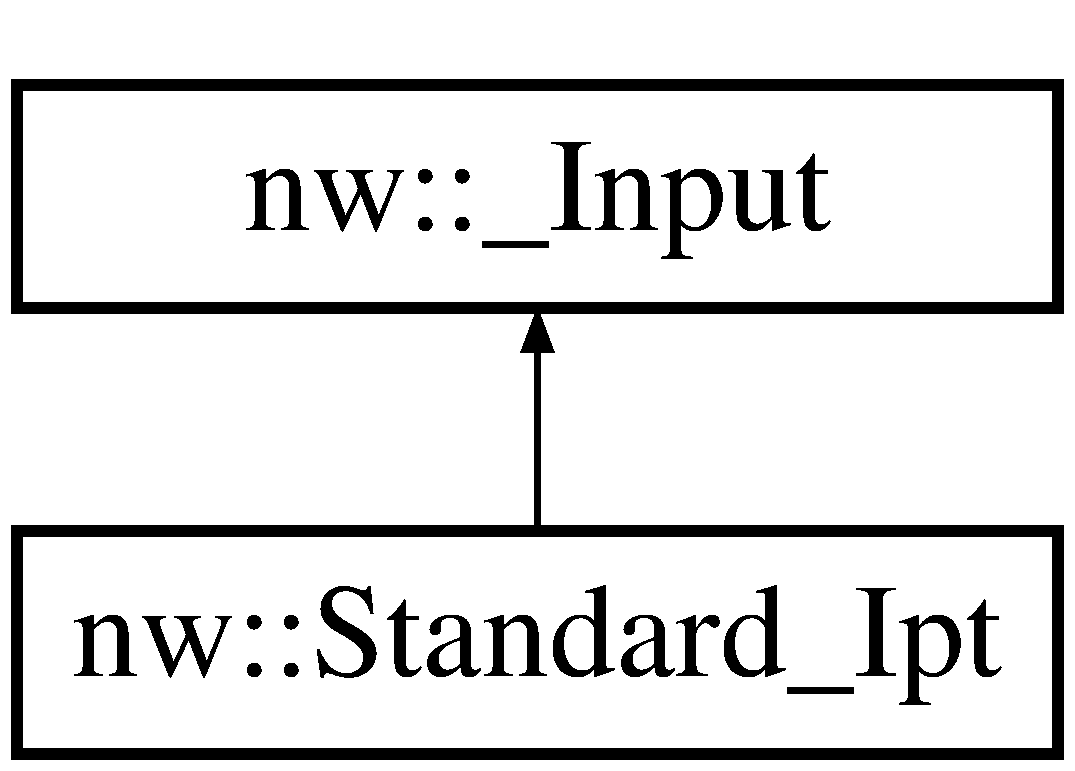
\includegraphics[height=2.000000cm]{dc/d65/classnw_1_1___input}
\end{center}
\end{figure}
\subsection*{Public Member Functions}
\begin{DoxyCompactItemize}
\item 
virtual \hyperlink{classnw_1_1___input_a6a1a98fe24120158898316797324d024}{$\sim$\+\_\+\+Input} ()
\item 
virtual \hyperlink{classnw_1_1___system}{nw\+::\+\_\+\+System} $\ast$ \hyperlink{classnw_1_1___input_a5bb57fdb6dfcf4efa7b64e096594a8b3}{get\+\_\+\+System} ()=0
\begin{DoxyCompactList}\small\item\em Translates input files into a \hyperlink{classnw_1_1___system}{\+\_\+\+System}. \end{DoxyCompactList}\end{DoxyCompactItemize}
\subsection*{Protected Attributes}
\begin{DoxyCompactItemize}
\item 
\hyperlink{classnw_1_1___system}{nw\+::\+\_\+\+System} $\ast$ \hyperlink{classnw_1_1___input_af4d5765ede8af8d7f981ef179683f7e5}{s}
\end{DoxyCompactItemize}


\subsection{Detailed Description}
Abstract base class for input procedures. 

Derivatives of {\ttfamily \hyperlink{classnw_1_1___input}{\+\_\+\+Input}} can implement different input interfaces to ensure compatibility with different input formats 

\subsection{Constructor \& Destructor Documentation}
\hypertarget{classnw_1_1___input_a6a1a98fe24120158898316797324d024}{\index{nw\+::\+\_\+\+Input@{nw\+::\+\_\+\+Input}!````~\+\_\+\+Input@{$\sim$\+\_\+\+Input}}
\index{````~\+\_\+\+Input@{$\sim$\+\_\+\+Input}!nw\+::\+\_\+\+Input@{nw\+::\+\_\+\+Input}}
\subsubsection[{$\sim$\+\_\+\+Input}]{\setlength{\rightskip}{0pt plus 5cm}virtual nw\+::\+\_\+\+Input\+::$\sim$\+\_\+\+Input (
\begin{DoxyParamCaption}
{}
\end{DoxyParamCaption}
)\hspace{0.3cm}{\ttfamily [inline]}, {\ttfamily [virtual]}}}\label{classnw_1_1___input_a6a1a98fe24120158898316797324d024}

\begin{DoxyCode}
13 \{\};
\end{DoxyCode}


\subsection{Member Function Documentation}
\hypertarget{classnw_1_1___input_a5bb57fdb6dfcf4efa7b64e096594a8b3}{\index{nw\+::\+\_\+\+Input@{nw\+::\+\_\+\+Input}!get\+\_\+\+System@{get\+\_\+\+System}}
\index{get\+\_\+\+System@{get\+\_\+\+System}!nw\+::\+\_\+\+Input@{nw\+::\+\_\+\+Input}}
\subsubsection[{get\+\_\+\+System}]{\setlength{\rightskip}{0pt plus 5cm}virtual {\bf nw\+::\+\_\+\+System}$\ast$ nw\+::\+\_\+\+Input\+::get\+\_\+\+System (
\begin{DoxyParamCaption}
{}
\end{DoxyParamCaption}
)\hspace{0.3cm}{\ttfamily [pure virtual]}}}\label{classnw_1_1___input_a5bb57fdb6dfcf4efa7b64e096594a8b3}


Translates input files into a \hyperlink{classnw_1_1___system}{\+\_\+\+System}. 

\begin{DoxyReturn}{Returns}
\hyperlink{classnw_1_1___system}{\+\_\+\+System} based on an input file. 
\end{DoxyReturn}


Implemented in \hyperlink{classnw_1_1_standard___ipt_ae5ae0e8b67291839d71df934bfc17238}{nw\+::\+Standard\+\_\+\+Ipt}.



\subsection{Member Data Documentation}
\hypertarget{classnw_1_1___input_af4d5765ede8af8d7f981ef179683f7e5}{\index{nw\+::\+\_\+\+Input@{nw\+::\+\_\+\+Input}!s@{s}}
\index{s@{s}!nw\+::\+\_\+\+Input@{nw\+::\+\_\+\+Input}}
\subsubsection[{s}]{\setlength{\rightskip}{0pt plus 5cm}{\bf nw\+::\+\_\+\+System}$\ast$ nw\+::\+\_\+\+Input\+::s\hspace{0.3cm}{\ttfamily [protected]}}}\label{classnw_1_1___input_af4d5765ede8af8d7f981ef179683f7e5}


The documentation for this class was generated from the following file\+:\begin{DoxyCompactItemize}
\item 
Input/\hyperlink{___input_8h}{\+\_\+\+Input.\+h}\end{DoxyCompactItemize}

\hypertarget{classnw_1_1___random}{\section{nw\+:\+:\+\_\+\+Random Class Reference}
\label{classnw_1_1___random}\index{nw\+::\+\_\+\+Random@{nw\+::\+\_\+\+Random}}
}


abstract base class to define an interface for Random Generators  




{\ttfamily \#include $<$\+\_\+\+Random.\+h$>$}

Inheritance diagram for nw\+:\+:\+\_\+\+Random\+:\begin{figure}[H]
\begin{center}
\leavevmode
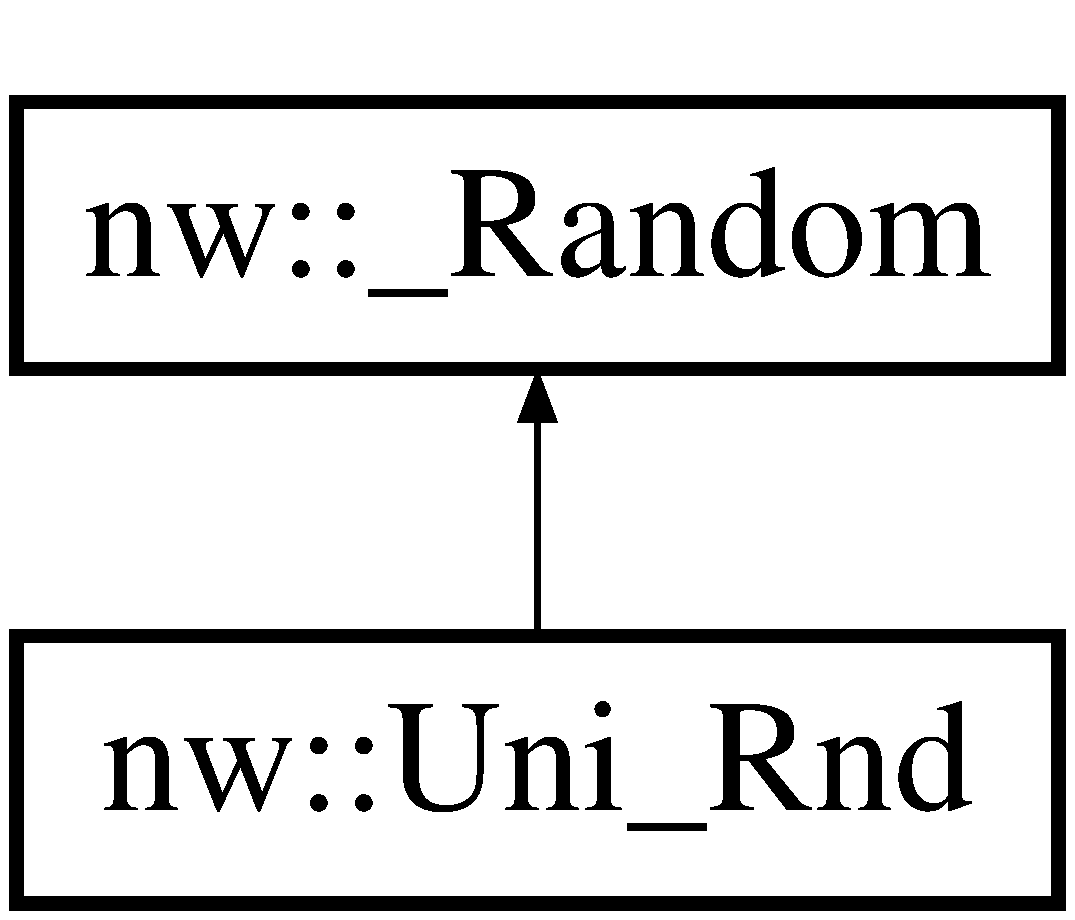
\includegraphics[height=2.000000cm]{db/da1/classnw_1_1___random}
\end{center}
\end{figure}
\subsection*{Public Member Functions}
\begin{DoxyCompactItemize}
\item 
virtual double \hyperlink{classnw_1_1___random_a943da227bd614e34718967a0521a51d1}{get\+\_\+\+Uni\+\_\+\+Rnd} ()=0
\begin{DoxyCompactList}\small\item\em Generate uniformly distributed random number between 0.\+0 and 1.\+0. \end{DoxyCompactList}\item 
virtual \hyperlink{classnw_1_1___random_a68b23d50878448edbeb2f9b61d9d36cd}{$\sim$\+\_\+\+Random} ()
\begin{DoxyCompactList}\small\item\em Destructor. \end{DoxyCompactList}\end{DoxyCompactItemize}
\subsection*{Private Attributes}
\begin{DoxyCompactItemize}
\item 
double \hyperlink{classnw_1_1___random_acfb88075bfcae45bbbd989568cef5250}{r}
\end{DoxyCompactItemize}


\subsection{Detailed Description}
abstract base class to define an interface for Random Generators 

\subsection{Constructor \& Destructor Documentation}
\hypertarget{classnw_1_1___random_a68b23d50878448edbeb2f9b61d9d36cd}{\index{nw\+::\+\_\+\+Random@{nw\+::\+\_\+\+Random}!````~\+\_\+\+Random@{$\sim$\+\_\+\+Random}}
\index{````~\+\_\+\+Random@{$\sim$\+\_\+\+Random}!nw\+::\+\_\+\+Random@{nw\+::\+\_\+\+Random}}
\subsubsection[{$\sim$\+\_\+\+Random}]{\setlength{\rightskip}{0pt plus 5cm}virtual nw\+::\+\_\+\+Random\+::$\sim$\+\_\+\+Random (
\begin{DoxyParamCaption}
{}
\end{DoxyParamCaption}
)\hspace{0.3cm}{\ttfamily [inline]}, {\ttfamily [virtual]}}}\label{classnw_1_1___random_a68b23d50878448edbeb2f9b61d9d36cd}


Destructor. 


\begin{DoxyCode}
13 \{\};
\end{DoxyCode}


\subsection{Member Function Documentation}
\hypertarget{classnw_1_1___random_a943da227bd614e34718967a0521a51d1}{\index{nw\+::\+\_\+\+Random@{nw\+::\+\_\+\+Random}!get\+\_\+\+Uni\+\_\+\+Rnd@{get\+\_\+\+Uni\+\_\+\+Rnd}}
\index{get\+\_\+\+Uni\+\_\+\+Rnd@{get\+\_\+\+Uni\+\_\+\+Rnd}!nw\+::\+\_\+\+Random@{nw\+::\+\_\+\+Random}}
\subsubsection[{get\+\_\+\+Uni\+\_\+\+Rnd}]{\setlength{\rightskip}{0pt plus 5cm}virtual double nw\+::\+\_\+\+Random\+::get\+\_\+\+Uni\+\_\+\+Rnd (
\begin{DoxyParamCaption}
{}
\end{DoxyParamCaption}
)\hspace{0.3cm}{\ttfamily [pure virtual]}}}\label{classnw_1_1___random_a943da227bd614e34718967a0521a51d1}


Generate uniformly distributed random number between 0.\+0 and 1.\+0. 

\begin{DoxyReturn}{Returns}
Uniformly distributed random number between 0.\+0 and 1.\+0 
\end{DoxyReturn}


Implemented in \hyperlink{classnw_1_1_uni___rnd_ad7883ef0ce4c591612bcb41678104773}{nw\+::\+Uni\+\_\+\+Rnd}.



\subsection{Member Data Documentation}
\hypertarget{classnw_1_1___random_acfb88075bfcae45bbbd989568cef5250}{\index{nw\+::\+\_\+\+Random@{nw\+::\+\_\+\+Random}!r@{r}}
\index{r@{r}!nw\+::\+\_\+\+Random@{nw\+::\+\_\+\+Random}}
\subsubsection[{r}]{\setlength{\rightskip}{0pt plus 5cm}double nw\+::\+\_\+\+Random\+::r\hspace{0.3cm}{\ttfamily [private]}}}\label{classnw_1_1___random_acfb88075bfcae45bbbd989568cef5250}


The documentation for this class was generated from the following file\+:\begin{DoxyCompactItemize}
\item 
Random/\hyperlink{___random_8h}{\+\_\+\+Random.\+h}\end{DoxyCompactItemize}

\hypertarget{classnw_1_1___species}{\section{nw\+:\+:\+\_\+\+Species Class Reference}
\label{classnw_1_1___species}\index{nw\+::\+\_\+\+Species@{nw\+::\+\_\+\+Species}}
}


Abstract base class for the molecular species of a system.  




{\ttfamily \#include $<$\+\_\+\+Species.\+h$>$}

Inheritance diagram for nw\+:\+:\+\_\+\+Species\+:\begin{figure}[H]
\begin{center}
\leavevmode
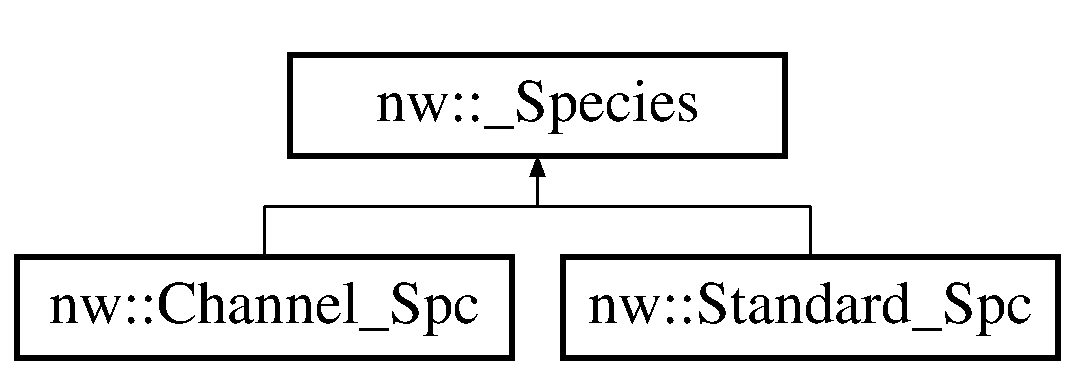
\includegraphics[height=2.000000cm]{d3/d03/classnw_1_1___species}
\end{center}
\end{figure}
\subsection*{Public Member Functions}
\begin{DoxyCompactItemize}
\item 
\hyperlink{classnw_1_1___species_af74ef3f4a59f3c8fa9ff6b1acc83be86}{\+\_\+\+Species} (long \hyperlink{classnw_1_1___species_ac42dfe1c656c17178a9649093519ebb7}{id}, string \hyperlink{classnw_1_1___species_a7b8ede09e28941beb48cf27f1247e2f9}{name}, double init\+\_\+conc)
\begin{DoxyCompactList}\small\item\em Constructor. \end{DoxyCompactList}\item 
virtual \hyperlink{classnw_1_1___species_aa3e9d32d88bf558cf6401d4b3dcf8f40}{$\sim$\+\_\+\+Species} ()
\begin{DoxyCompactList}\small\item\em Destructor. \end{DoxyCompactList}\item 
virtual long \hyperlink{classnw_1_1___species_a6e3e68477663ff511d75fb24cf01cb9f}{get\+\_\+n\+\_\+molecules} ()=0
\begin{DoxyCompactList}\small\item\em Get current number of molecules. \end{DoxyCompactList}\item 
virtual void \hyperlink{classnw_1_1___species_ac7955c9fe040d8cae8f3cae4684ed96b}{mod\+\_\+n\+\_\+molecules} (long n)=0
\begin{DoxyCompactList}\small\item\em Modify number of molecules (n\+\_\+molecules). \end{DoxyCompactList}\item 
virtual \hyperlink{classnw_1_1___species}{\+\_\+\+Species} $\ast$ \hyperlink{classnw_1_1___species_aea43d96b0b1c9e88953f40fbe58e7f29}{copy} ()=0
\begin{DoxyCompactList}\small\item\em Copy method. \end{DoxyCompactList}\item 
virtual void \hyperlink{classnw_1_1___species_a53d06cca549a83bfff71303174707926}{set\+\_\+n\+\_\+molecules} (double \hyperlink{classnw_1_1___species_a80896a55f086f468396e76ae8f1e8285}{volume})
\begin{DoxyCompactList}\small\item\em Set initial molecular count (n\+\_\+molecules). \end{DoxyCompactList}\item 
long \hyperlink{classnw_1_1___species_a03f4b80da067d1bb6e2ab2d74e3f49d9}{get\+\_\+id} ()
\item 
string \hyperlink{classnw_1_1___species_ab52e303fd75637ca239b96a1efcd0bf4}{get\+\_\+name} ()
\item 
double \hyperlink{classnw_1_1___species_a8246da49ed5c2ce46365e5bd15025a1c}{get\+\_\+initial\+\_\+conc} ()
\item 
bool \hyperlink{classnw_1_1___species_a89fb2e72e485dd2f7fed07cfcfa7cdb0}{get\+\_\+dirty\+\_\+flag} ()
\item 
void \hyperlink{classnw_1_1___species_a9c52abce36663e6df5b51197282e0de3}{set\+\_\+dirty\+\_\+flag} (bool b)
\end{DoxyCompactItemize}
\subsection*{Protected Attributes}
\begin{DoxyCompactItemize}
\item 
long \hyperlink{classnw_1_1___species_ac42dfe1c656c17178a9649093519ebb7}{id}
\begin{DoxyCompactList}\small\item\em Species I\+D. \end{DoxyCompactList}\item 
string \hyperlink{classnw_1_1___species_a7b8ede09e28941beb48cf27f1247e2f9}{name}
\begin{DoxyCompactList}\small\item\em Species name. \end{DoxyCompactList}\item 
bool \hyperlink{classnw_1_1___species_a79157bae3920ce7bba35e3f75b2aad6f}{dirty\+\_\+flag}
\begin{DoxyCompactList}\small\item\em Indicates whether this \hyperlink{classnw_1_1___species}{\+\_\+\+Species} needs to be updated or not. \end{DoxyCompactList}\item 
long \hyperlink{classnw_1_1___species_af6ae0232b4f994b464a2f69cb022b33f}{n\+\_\+molecules}
\begin{DoxyCompactList}\small\item\em Current number of molecules. \end{DoxyCompactList}\item 
double \hyperlink{classnw_1_1___species_ac66cdd3bdd5be88791e00d063b4e92a2}{initial\+\_\+conc}
\begin{DoxyCompactList}\small\item\em Initial concentration. \end{DoxyCompactList}\item 
double \hyperlink{classnw_1_1___species_a80896a55f086f468396e76ae8f1e8285}{volume}
\begin{DoxyCompactList}\small\item\em Volume of the \hyperlink{classnw_1_1___voxel}{\+\_\+\+Voxel} containing this \hyperlink{classnw_1_1___species}{\+\_\+\+Species}. \end{DoxyCompactList}\end{DoxyCompactItemize}


\subsection{Detailed Description}
Abstract base class for the molecular species of a system. 

\subsection{Constructor \& Destructor Documentation}
\hypertarget{classnw_1_1___species_af74ef3f4a59f3c8fa9ff6b1acc83be86}{\index{nw\+::\+\_\+\+Species@{nw\+::\+\_\+\+Species}!\+\_\+\+Species@{\+\_\+\+Species}}
\index{\+\_\+\+Species@{\+\_\+\+Species}!nw\+::\+\_\+\+Species@{nw\+::\+\_\+\+Species}}
\subsubsection[{\+\_\+\+Species}]{\setlength{\rightskip}{0pt plus 5cm}nw\+::\+\_\+\+Species\+::\+\_\+\+Species (
\begin{DoxyParamCaption}
\item[{long}]{id, }
\item[{string}]{name, }
\item[{double}]{init\+\_\+conc}
\end{DoxyParamCaption}
)\hspace{0.3cm}{\ttfamily [inline]}}}\label{classnw_1_1___species_af74ef3f4a59f3c8fa9ff6b1acc83be86}


Constructor. 


\begin{DoxyParams}{Parameters}
{\em id} & Species I\+D \\
\hline
{\em name} & Species name \\
\hline
{\em init\+\_\+conc} & initial concentration \\
\hline
\end{DoxyParams}

\begin{DoxyCode}
24                                                    :
25         \hyperlink{classnw_1_1___species_ac42dfe1c656c17178a9649093519ebb7}{id}(\textcolor{keywordtype}{id}),
26         \hyperlink{classnw_1_1___species_a7b8ede09e28941beb48cf27f1247e2f9}{name}(\hyperlink{classnw_1_1___species_a7b8ede09e28941beb48cf27f1247e2f9}{name}),
27         \hyperlink{classnw_1_1___species_a79157bae3920ce7bba35e3f75b2aad6f}{dirty\_flag}(\textcolor{keyword}{true}),
28         \hyperlink{classnw_1_1___species_ac66cdd3bdd5be88791e00d063b4e92a2}{initial\_conc}(init\_conc) \{\}
\end{DoxyCode}
\hypertarget{classnw_1_1___species_aa3e9d32d88bf558cf6401d4b3dcf8f40}{\index{nw\+::\+\_\+\+Species@{nw\+::\+\_\+\+Species}!````~\+\_\+\+Species@{$\sim$\+\_\+\+Species}}
\index{````~\+\_\+\+Species@{$\sim$\+\_\+\+Species}!nw\+::\+\_\+\+Species@{nw\+::\+\_\+\+Species}}
\subsubsection[{$\sim$\+\_\+\+Species}]{\setlength{\rightskip}{0pt plus 5cm}virtual nw\+::\+\_\+\+Species\+::$\sim$\+\_\+\+Species (
\begin{DoxyParamCaption}
{}
\end{DoxyParamCaption}
)\hspace{0.3cm}{\ttfamily [inline]}, {\ttfamily [virtual]}}}\label{classnw_1_1___species_aa3e9d32d88bf558cf6401d4b3dcf8f40}


Destructor. 


\begin{DoxyCode}
30 \{\};
\end{DoxyCode}


\subsection{Member Function Documentation}
\hypertarget{classnw_1_1___species_aea43d96b0b1c9e88953f40fbe58e7f29}{\index{nw\+::\+\_\+\+Species@{nw\+::\+\_\+\+Species}!copy@{copy}}
\index{copy@{copy}!nw\+::\+\_\+\+Species@{nw\+::\+\_\+\+Species}}
\subsubsection[{copy}]{\setlength{\rightskip}{0pt plus 5cm}virtual {\bf \+\_\+\+Species}$\ast$ nw\+::\+\_\+\+Species\+::copy (
\begin{DoxyParamCaption}
{}
\end{DoxyParamCaption}
)\hspace{0.3cm}{\ttfamily [pure virtual]}}}\label{classnw_1_1___species_aea43d96b0b1c9e88953f40fbe58e7f29}


Copy method. 

\begin{DoxyReturn}{Returns}
Reference to an object identical to this
\end{DoxyReturn}
Copy method that generates a copy of this. It is is a virtual function to ensure that whenever this function is called, the most specific object (derived from this abstract base class) is copied. 

Implemented in \hyperlink{classnw_1_1_channel___spc_ab35f288a4021c302b4e2dc09e54578b1}{nw\+::\+Channel\+\_\+\+Spc}, and \hyperlink{classnw_1_1_standard___spc_abc6e6a61ebdcd1e1b917c3e3a5f9cd24}{nw\+::\+Standard\+\_\+\+Spc}.

\hypertarget{classnw_1_1___species_a89fb2e72e485dd2f7fed07cfcfa7cdb0}{\index{nw\+::\+\_\+\+Species@{nw\+::\+\_\+\+Species}!get\+\_\+dirty\+\_\+flag@{get\+\_\+dirty\+\_\+flag}}
\index{get\+\_\+dirty\+\_\+flag@{get\+\_\+dirty\+\_\+flag}!nw\+::\+\_\+\+Species@{nw\+::\+\_\+\+Species}}
\subsubsection[{get\+\_\+dirty\+\_\+flag}]{\setlength{\rightskip}{0pt plus 5cm}bool nw\+::\+\_\+\+Species\+::get\+\_\+dirty\+\_\+flag (
\begin{DoxyParamCaption}
{}
\end{DoxyParamCaption}
)\hspace{0.3cm}{\ttfamily [inline]}}}\label{classnw_1_1___species_a89fb2e72e485dd2f7fed07cfcfa7cdb0}

\begin{DoxyCode}
60 \{\textcolor{keywordflow}{return} \hyperlink{classnw_1_1___species_a79157bae3920ce7bba35e3f75b2aad6f}{dirty\_flag};\}
\end{DoxyCode}
\hypertarget{classnw_1_1___species_a03f4b80da067d1bb6e2ab2d74e3f49d9}{\index{nw\+::\+\_\+\+Species@{nw\+::\+\_\+\+Species}!get\+\_\+id@{get\+\_\+id}}
\index{get\+\_\+id@{get\+\_\+id}!nw\+::\+\_\+\+Species@{nw\+::\+\_\+\+Species}}
\subsubsection[{get\+\_\+id}]{\setlength{\rightskip}{0pt plus 5cm}long nw\+::\+\_\+\+Species\+::get\+\_\+id (
\begin{DoxyParamCaption}
{}
\end{DoxyParamCaption}
)\hspace{0.3cm}{\ttfamily [inline]}}}\label{classnw_1_1___species_a03f4b80da067d1bb6e2ab2d74e3f49d9}

\begin{DoxyCode}
57 \{\textcolor{keywordflow}{return} \hyperlink{classnw_1_1___species_ac42dfe1c656c17178a9649093519ebb7}{id};\}
\end{DoxyCode}
\hypertarget{classnw_1_1___species_a8246da49ed5c2ce46365e5bd15025a1c}{\index{nw\+::\+\_\+\+Species@{nw\+::\+\_\+\+Species}!get\+\_\+initial\+\_\+conc@{get\+\_\+initial\+\_\+conc}}
\index{get\+\_\+initial\+\_\+conc@{get\+\_\+initial\+\_\+conc}!nw\+::\+\_\+\+Species@{nw\+::\+\_\+\+Species}}
\subsubsection[{get\+\_\+initial\+\_\+conc}]{\setlength{\rightskip}{0pt plus 5cm}double nw\+::\+\_\+\+Species\+::get\+\_\+initial\+\_\+conc (
\begin{DoxyParamCaption}
{}
\end{DoxyParamCaption}
)\hspace{0.3cm}{\ttfamily [inline]}}}\label{classnw_1_1___species_a8246da49ed5c2ce46365e5bd15025a1c}

\begin{DoxyCode}
59 \{\textcolor{keywordflow}{return} \hyperlink{classnw_1_1___species_ac66cdd3bdd5be88791e00d063b4e92a2}{initial\_conc};\}
\end{DoxyCode}
\hypertarget{classnw_1_1___species_a6e3e68477663ff511d75fb24cf01cb9f}{\index{nw\+::\+\_\+\+Species@{nw\+::\+\_\+\+Species}!get\+\_\+n\+\_\+molecules@{get\+\_\+n\+\_\+molecules}}
\index{get\+\_\+n\+\_\+molecules@{get\+\_\+n\+\_\+molecules}!nw\+::\+\_\+\+Species@{nw\+::\+\_\+\+Species}}
\subsubsection[{get\+\_\+n\+\_\+molecules}]{\setlength{\rightskip}{0pt plus 5cm}virtual long nw\+::\+\_\+\+Species\+::get\+\_\+n\+\_\+molecules (
\begin{DoxyParamCaption}
{}
\end{DoxyParamCaption}
)\hspace{0.3cm}{\ttfamily [pure virtual]}}}\label{classnw_1_1___species_a6e3e68477663ff511d75fb24cf01cb9f}


Get current number of molecules. 

\begin{DoxyReturn}{Returns}
current number of molecules 
\end{DoxyReturn}


Implemented in \hyperlink{classnw_1_1_channel___spc_a20a1e6dd089794ad0e1035635a1e3fe0}{nw\+::\+Channel\+\_\+\+Spc}, and \hyperlink{classnw_1_1_standard___spc_aa1b07cee6c86dd83aa9970c0964d16fc}{nw\+::\+Standard\+\_\+\+Spc}.

\hypertarget{classnw_1_1___species_ab52e303fd75637ca239b96a1efcd0bf4}{\index{nw\+::\+\_\+\+Species@{nw\+::\+\_\+\+Species}!get\+\_\+name@{get\+\_\+name}}
\index{get\+\_\+name@{get\+\_\+name}!nw\+::\+\_\+\+Species@{nw\+::\+\_\+\+Species}}
\subsubsection[{get\+\_\+name}]{\setlength{\rightskip}{0pt plus 5cm}string nw\+::\+\_\+\+Species\+::get\+\_\+name (
\begin{DoxyParamCaption}
{}
\end{DoxyParamCaption}
)\hspace{0.3cm}{\ttfamily [inline]}}}\label{classnw_1_1___species_ab52e303fd75637ca239b96a1efcd0bf4}

\begin{DoxyCode}
58 \{\textcolor{keywordflow}{return} \hyperlink{classnw_1_1___species_a7b8ede09e28941beb48cf27f1247e2f9}{name};\}
\end{DoxyCode}
\hypertarget{classnw_1_1___species_ac7955c9fe040d8cae8f3cae4684ed96b}{\index{nw\+::\+\_\+\+Species@{nw\+::\+\_\+\+Species}!mod\+\_\+n\+\_\+molecules@{mod\+\_\+n\+\_\+molecules}}
\index{mod\+\_\+n\+\_\+molecules@{mod\+\_\+n\+\_\+molecules}!nw\+::\+\_\+\+Species@{nw\+::\+\_\+\+Species}}
\subsubsection[{mod\+\_\+n\+\_\+molecules}]{\setlength{\rightskip}{0pt plus 5cm}virtual void nw\+::\+\_\+\+Species\+::mod\+\_\+n\+\_\+molecules (
\begin{DoxyParamCaption}
\item[{long}]{n}
\end{DoxyParamCaption}
)\hspace{0.3cm}{\ttfamily [pure virtual]}}}\label{classnw_1_1___species_ac7955c9fe040d8cae8f3cae4684ed96b}


Modify number of molecules (n\+\_\+molecules). 


\begin{DoxyParams}{Parameters}
{\em n} & Summand that is added to the current number of molecules.\\
\hline
\end{DoxyParams}
If an event occurs, this function is called to update the number of molecules based on the state change vector of the firing \hyperlink{classnw_1_1___event}{\+\_\+\+Event}. If {\ttfamily n} is positive the number of molecules is increased, if it is negative the number of molecules in decrease. 

Implemented in \hyperlink{classnw_1_1_channel___spc_a03347a88efec50ad3acd0ff4025ed23d}{nw\+::\+Channel\+\_\+\+Spc}, and \hyperlink{classnw_1_1_standard___spc_aed4c0ba53c924011269b59a4a5181fe4}{nw\+::\+Standard\+\_\+\+Spc}.

\hypertarget{classnw_1_1___species_a9c52abce36663e6df5b51197282e0de3}{\index{nw\+::\+\_\+\+Species@{nw\+::\+\_\+\+Species}!set\+\_\+dirty\+\_\+flag@{set\+\_\+dirty\+\_\+flag}}
\index{set\+\_\+dirty\+\_\+flag@{set\+\_\+dirty\+\_\+flag}!nw\+::\+\_\+\+Species@{nw\+::\+\_\+\+Species}}
\subsubsection[{set\+\_\+dirty\+\_\+flag}]{\setlength{\rightskip}{0pt plus 5cm}void nw\+::\+\_\+\+Species\+::set\+\_\+dirty\+\_\+flag (
\begin{DoxyParamCaption}
\item[{bool}]{b}
\end{DoxyParamCaption}
)\hspace{0.3cm}{\ttfamily [inline]}}}\label{classnw_1_1___species_a9c52abce36663e6df5b51197282e0de3}

\begin{DoxyCode}
61 \{\hyperlink{classnw_1_1___species_a79157bae3920ce7bba35e3f75b2aad6f}{dirty\_flag} = b;\}
\end{DoxyCode}
\hypertarget{classnw_1_1___species_a53d06cca549a83bfff71303174707926}{\index{nw\+::\+\_\+\+Species@{nw\+::\+\_\+\+Species}!set\+\_\+n\+\_\+molecules@{set\+\_\+n\+\_\+molecules}}
\index{set\+\_\+n\+\_\+molecules@{set\+\_\+n\+\_\+molecules}!nw\+::\+\_\+\+Species@{nw\+::\+\_\+\+Species}}
\subsubsection[{set\+\_\+n\+\_\+molecules}]{\setlength{\rightskip}{0pt plus 5cm}virtual void nw\+::\+\_\+\+Species\+::set\+\_\+n\+\_\+molecules (
\begin{DoxyParamCaption}
\item[{double}]{volume}
\end{DoxyParamCaption}
)\hspace{0.3cm}{\ttfamily [inline]}, {\ttfamily [virtual]}}}\label{classnw_1_1___species_a53d06cca549a83bfff71303174707926}


Set initial molecular count (n\+\_\+molecules). 

Called in the constructor of every \hyperlink{classnw_1_1___voxel}{\+\_\+\+Voxel} to set the correct (\hyperlink{classnw_1_1___voxel}{\+\_\+\+Voxel} volume adapted) number of molecules. This makes it easier to define \hyperlink{classnw_1_1___species}{\+\_\+\+Species} and \hyperlink{classnw_1_1___voxel}{\+\_\+\+Voxel} in the input file. 

Reimplemented in \hyperlink{classnw_1_1_channel___spc_af8d5d7097d343e6646c6c11a1744024d}{nw\+::\+Channel\+\_\+\+Spc}.


\begin{DoxyCode}
53                                                \{
54         this->\hyperlink{classnw_1_1___species_af6ae0232b4f994b464a2f69cb022b33f}{n\_molecules} = \hyperlink{classnw_1_1___species_a80896a55f086f468396e76ae8f1e8285}{volume}*1e-6*\hyperlink{namespacenw_ad890cfa7dd9eaf8d5b6754723e516c4a}{N\_AVO}*\hyperlink{classnw_1_1___species_ac66cdd3bdd5be88791e00d063b4e92a2}{initial\_conc};\}
\end{DoxyCode}


\subsection{Member Data Documentation}
\hypertarget{classnw_1_1___species_a79157bae3920ce7bba35e3f75b2aad6f}{\index{nw\+::\+\_\+\+Species@{nw\+::\+\_\+\+Species}!dirty\+\_\+flag@{dirty\+\_\+flag}}
\index{dirty\+\_\+flag@{dirty\+\_\+flag}!nw\+::\+\_\+\+Species@{nw\+::\+\_\+\+Species}}
\subsubsection[{dirty\+\_\+flag}]{\setlength{\rightskip}{0pt plus 5cm}bool nw\+::\+\_\+\+Species\+::dirty\+\_\+flag\hspace{0.3cm}{\ttfamily [protected]}}}\label{classnw_1_1___species_a79157bae3920ce7bba35e3f75b2aad6f}


Indicates whether this \hyperlink{classnw_1_1___species}{\+\_\+\+Species} needs to be updated or not. 

\hypertarget{classnw_1_1___species_ac42dfe1c656c17178a9649093519ebb7}{\index{nw\+::\+\_\+\+Species@{nw\+::\+\_\+\+Species}!id@{id}}
\index{id@{id}!nw\+::\+\_\+\+Species@{nw\+::\+\_\+\+Species}}
\subsubsection[{id}]{\setlength{\rightskip}{0pt plus 5cm}long nw\+::\+\_\+\+Species\+::id\hspace{0.3cm}{\ttfamily [protected]}}}\label{classnw_1_1___species_ac42dfe1c656c17178a9649093519ebb7}


Species I\+D. 

\hypertarget{classnw_1_1___species_ac66cdd3bdd5be88791e00d063b4e92a2}{\index{nw\+::\+\_\+\+Species@{nw\+::\+\_\+\+Species}!initial\+\_\+conc@{initial\+\_\+conc}}
\index{initial\+\_\+conc@{initial\+\_\+conc}!nw\+::\+\_\+\+Species@{nw\+::\+\_\+\+Species}}
\subsubsection[{initial\+\_\+conc}]{\setlength{\rightskip}{0pt plus 5cm}double nw\+::\+\_\+\+Species\+::initial\+\_\+conc\hspace{0.3cm}{\ttfamily [protected]}}}\label{classnw_1_1___species_ac66cdd3bdd5be88791e00d063b4e92a2}


Initial concentration. 

\hypertarget{classnw_1_1___species_af6ae0232b4f994b464a2f69cb022b33f}{\index{nw\+::\+\_\+\+Species@{nw\+::\+\_\+\+Species}!n\+\_\+molecules@{n\+\_\+molecules}}
\index{n\+\_\+molecules@{n\+\_\+molecules}!nw\+::\+\_\+\+Species@{nw\+::\+\_\+\+Species}}
\subsubsection[{n\+\_\+molecules}]{\setlength{\rightskip}{0pt plus 5cm}long nw\+::\+\_\+\+Species\+::n\+\_\+molecules\hspace{0.3cm}{\ttfamily [protected]}}}\label{classnw_1_1___species_af6ae0232b4f994b464a2f69cb022b33f}


Current number of molecules. 

\hypertarget{classnw_1_1___species_a7b8ede09e28941beb48cf27f1247e2f9}{\index{nw\+::\+\_\+\+Species@{nw\+::\+\_\+\+Species}!name@{name}}
\index{name@{name}!nw\+::\+\_\+\+Species@{nw\+::\+\_\+\+Species}}
\subsubsection[{name}]{\setlength{\rightskip}{0pt plus 5cm}string nw\+::\+\_\+\+Species\+::name\hspace{0.3cm}{\ttfamily [protected]}}}\label{classnw_1_1___species_a7b8ede09e28941beb48cf27f1247e2f9}


Species name. 

\hypertarget{classnw_1_1___species_a80896a55f086f468396e76ae8f1e8285}{\index{nw\+::\+\_\+\+Species@{nw\+::\+\_\+\+Species}!volume@{volume}}
\index{volume@{volume}!nw\+::\+\_\+\+Species@{nw\+::\+\_\+\+Species}}
\subsubsection[{volume}]{\setlength{\rightskip}{0pt plus 5cm}double nw\+::\+\_\+\+Species\+::volume\hspace{0.3cm}{\ttfamily [protected]}}}\label{classnw_1_1___species_a80896a55f086f468396e76ae8f1e8285}


Volume of the \hyperlink{classnw_1_1___voxel}{\+\_\+\+Voxel} containing this \hyperlink{classnw_1_1___species}{\+\_\+\+Species}. 



The documentation for this class was generated from the following file\+:\begin{DoxyCompactItemize}
\item 
Species/\hyperlink{___species_8h}{\+\_\+\+Species.\+h}\end{DoxyCompactItemize}

\hypertarget{classnw_1_1___system}{\section{nw\+:\+:\+\_\+\+System Class Reference}
\label{classnw_1_1___system}\index{nw\+::\+\_\+\+System@{nw\+::\+\_\+\+System}}
}


Abstract base class for the implementation of simulation algorithms.  




{\ttfamily \#include $<$\+\_\+\+System.\+h$>$}

Inheritance diagram for nw\+:\+:\+\_\+\+System\+:\begin{figure}[H]
\begin{center}
\leavevmode
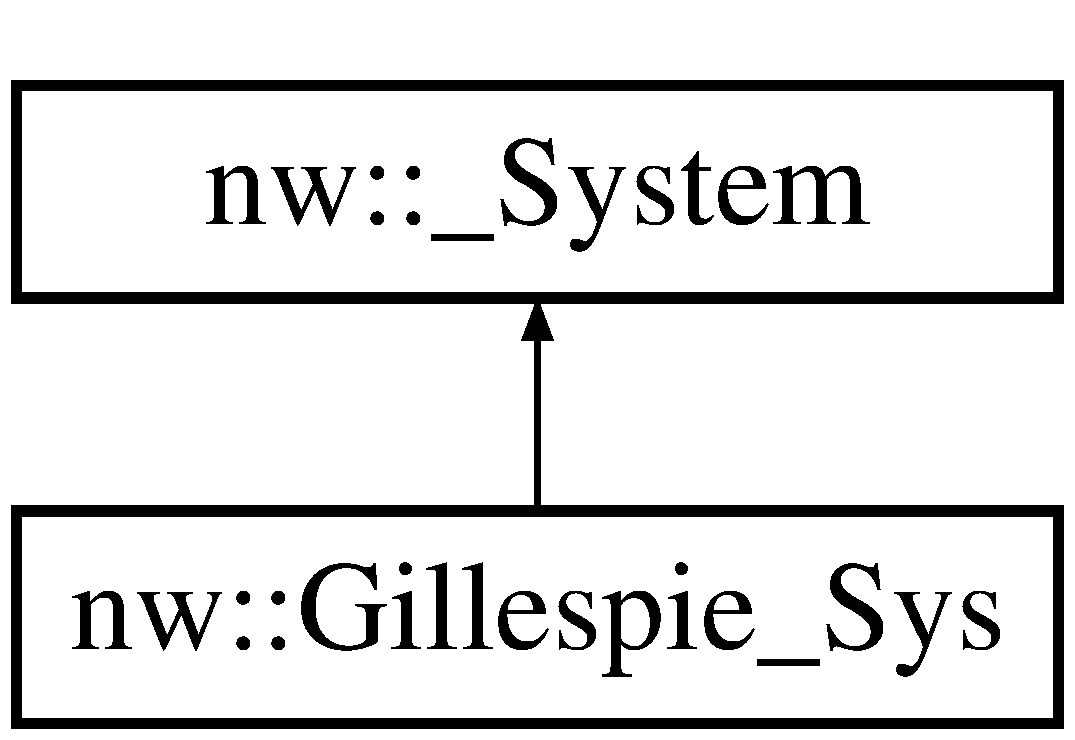
\includegraphics[height=2.000000cm]{d4/d68/classnw_1_1___system}
\end{center}
\end{figure}
\subsection*{Public Member Functions}
\begin{DoxyCompactItemize}
\item 
\hyperlink{classnw_1_1___system_aecf5603295f3d88f2767aadf25db202a}{\+\_\+\+System} ()
\item 
virtual \hyperlink{classnw_1_1___system_a450424d880a58f8b1e4c460357b2356b}{$\sim$\+\_\+\+System} ()
\item 
virtual void \hyperlink{classnw_1_1___system_ae0276aebba39a971d6e240a86a389713}{go} (long n\+\_\+it)=0
\begin{DoxyCompactList}\small\item\em executes simulation algorithm \end{DoxyCompactList}\end{DoxyCompactItemize}


\subsection{Detailed Description}
Abstract base class for the implementation of simulation algorithms. 

Algorithms integrated in this software framework are derived from \hyperlink{classnw_1_1___system}{\+\_\+\+System}. It solely requires the existence of the function \hyperlink{classnw_1_1___system_ae0276aebba39a971d6e240a86a389713}{go()} that executes the algorithm. 

\subsection{Constructor \& Destructor Documentation}
\hypertarget{classnw_1_1___system_aecf5603295f3d88f2767aadf25db202a}{\index{nw\+::\+\_\+\+System@{nw\+::\+\_\+\+System}!\+\_\+\+System@{\+\_\+\+System}}
\index{\+\_\+\+System@{\+\_\+\+System}!nw\+::\+\_\+\+System@{nw\+::\+\_\+\+System}}
\subsubsection[{\+\_\+\+System}]{\setlength{\rightskip}{0pt plus 5cm}nw\+::\+\_\+\+System\+::\+\_\+\+System (
\begin{DoxyParamCaption}
{}
\end{DoxyParamCaption}
)\hspace{0.3cm}{\ttfamily [inline]}}}\label{classnw_1_1___system_aecf5603295f3d88f2767aadf25db202a}

\begin{DoxyCode}
13 \{\};
\end{DoxyCode}
\hypertarget{classnw_1_1___system_a450424d880a58f8b1e4c460357b2356b}{\index{nw\+::\+\_\+\+System@{nw\+::\+\_\+\+System}!````~\+\_\+\+System@{$\sim$\+\_\+\+System}}
\index{````~\+\_\+\+System@{$\sim$\+\_\+\+System}!nw\+::\+\_\+\+System@{nw\+::\+\_\+\+System}}
\subsubsection[{$\sim$\+\_\+\+System}]{\setlength{\rightskip}{0pt plus 5cm}virtual nw\+::\+\_\+\+System\+::$\sim$\+\_\+\+System (
\begin{DoxyParamCaption}
{}
\end{DoxyParamCaption}
)\hspace{0.3cm}{\ttfamily [inline]}, {\ttfamily [virtual]}}}\label{classnw_1_1___system_a450424d880a58f8b1e4c460357b2356b}

\begin{DoxyCode}
14 \{\};
\end{DoxyCode}


\subsection{Member Function Documentation}
\hypertarget{classnw_1_1___system_ae0276aebba39a971d6e240a86a389713}{\index{nw\+::\+\_\+\+System@{nw\+::\+\_\+\+System}!go@{go}}
\index{go@{go}!nw\+::\+\_\+\+System@{nw\+::\+\_\+\+System}}
\subsubsection[{go}]{\setlength{\rightskip}{0pt plus 5cm}virtual void nw\+::\+\_\+\+System\+::go (
\begin{DoxyParamCaption}
\item[{long}]{n\+\_\+it}
\end{DoxyParamCaption}
)\hspace{0.3cm}{\ttfamily [pure virtual]}}}\label{classnw_1_1___system_ae0276aebba39a971d6e240a86a389713}


executes simulation algorithm 


\begin{DoxyParams}{Parameters}
{\em n\+\_\+it} & Current number of simulation run (required for output file names to distinguish between multiple trajectories resulting from multiple simulation runs during one program call.) \\
\hline
\end{DoxyParams}


Implemented in \hyperlink{classnw_1_1_gillespie___sys_ad21aa35a51bac13fe64dc6d838e77aee}{nw\+::\+Gillespie\+\_\+\+Sys}.



The documentation for this class was generated from the following file\+:\begin{DoxyCompactItemize}
\item 
System/\hyperlink{___system_8h}{\+\_\+\+System.\+h}\end{DoxyCompactItemize}

\hypertarget{classnw_1_1___voxel}{\section{nw\+:\+:\+\_\+\+Voxel Class Reference}
\label{classnw_1_1___voxel}\index{nw\+::\+\_\+\+Voxel@{nw\+::\+\_\+\+Voxel}}
}


Abstract base class for voxel (discrete building blocks of the simulation volume)  




{\ttfamily \#include $<$\+\_\+\+Voxel.\+h$>$}

Inheritance diagram for nw\+:\+:\+\_\+\+Voxel\+:\begin{figure}[H]
\begin{center}
\leavevmode
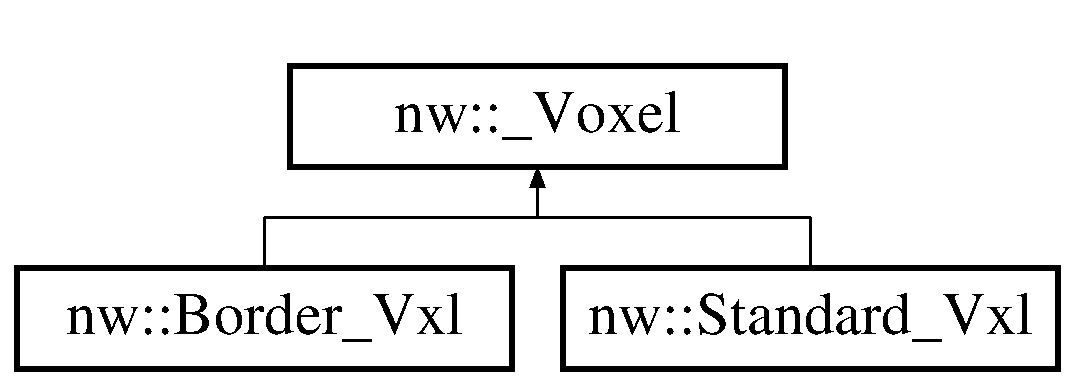
\includegraphics[height=2.000000cm]{d3/d7a/classnw_1_1___voxel}
\end{center}
\end{figure}
\subsection*{Public Member Functions}
\begin{DoxyCompactItemize}
\item 
\hyperlink{classnw_1_1___voxel_a0622dd383528f5115c6a450b6cbb1b34}{\+\_\+\+Voxel} (long \hyperlink{classnw_1_1___voxel_a01b73aff9af26230df4c483c5bd81896}{id}, double \hyperlink{classnw_1_1___voxel_ad9c3dbd0ea989af6ba7e1b5e09f6a989}{box\+\_\+length}, \hyperlink{namespacenw_a68aa8285591d78ebfc793c531bd43a23}{Species\+Vector} \hyperlink{classnw_1_1___voxel_a7762f59802c2a0b54bd18acbf803ff34}{state\+\_\+vec})
\begin{DoxyCompactList}\small\item\em Constructor. \end{DoxyCompactList}\item 
virtual \hyperlink{classnw_1_1___voxel_ac179b9c8ef72a7bef8ba54a89fcfa4a9}{$\sim$\+\_\+\+Voxel} ()
\begin{DoxyCompactList}\small\item\em Destructor. \end{DoxyCompactList}\item 
virtual void \hyperlink{classnw_1_1___voxel_a5842ac3c24bda907204852db0cf46810}{update\+\_\+state} (vector$<$ long $>$ sc\+\_\+vec)=0
\begin{DoxyCompactList}\small\item\em Update the state vector of voxel. \end{DoxyCompactList}\item 
void \hyperlink{classnw_1_1___voxel_a09cd07ce7f9099eed8820e5c5f2b3977}{clean} ()
\begin{DoxyCompactList}\small\item\em Clean dirty flag (set dirty\+\_\+flag = false). \end{DoxyCompactList}\item 
void \hyperlink{classnw_1_1___voxel_a86f184c141fa863b796e9248222be7e9}{add\+\_\+neighbour} (\hyperlink{classnw_1_1___voxel}{\+\_\+\+Voxel} $\ast$v)
\begin{DoxyCompactList}\small\item\em Add voxel to diffusion vector. \end{DoxyCompactList}\item 
bool \hyperlink{classnw_1_1___voxel_aff78d5b2069500df3116fbc0b4c767a0}{get\+\_\+dirty\+\_\+flag} ()
\item 
double \hyperlink{classnw_1_1___voxel_a6c420e07f31de22e981f933a36a57b22}{get\+\_\+volume} ()
\item 
double \hyperlink{classnw_1_1___voxel_a836eab78d769eae2b732335a91d84148}{get\+\_\+box\+\_\+length} ()
\item 
long \hyperlink{classnw_1_1___voxel_a0336ad5b120b40c4ad3f0012f50def1b}{get\+\_\+id} ()
\item 
\hyperlink{namespacenw_a68aa8285591d78ebfc793c531bd43a23}{Species\+Vector} $\ast$ \hyperlink{classnw_1_1___voxel_a91f1d799645722bf5fe15c34137433b1}{get\+\_\+state\+\_\+vec} ()
\item 
vector$<$ \hyperlink{classnw_1_1___voxel}{\+\_\+\+Voxel} $\ast$ $>$ $\ast$ \hyperlink{classnw_1_1___voxel_a688c8c9ca0a3a533e557a800d9f3b511}{get\+\_\+diff\+\_\+vec} ()
\end{DoxyCompactItemize}
\subsection*{Protected Attributes}
\begin{DoxyCompactItemize}
\item 
long \hyperlink{classnw_1_1___voxel_a01b73aff9af26230df4c483c5bd81896}{id}
\begin{DoxyCompactList}\small\item\em \hyperlink{classnw_1_1___voxel}{\+\_\+\+Voxel} I\+D \end{DoxyCompactList}\item 
double \hyperlink{classnw_1_1___voxel_ad9c3dbd0ea989af6ba7e1b5e09f6a989}{box\+\_\+length}
\begin{DoxyCompactList}\small\item\em \hyperlink{classnw_1_1___voxel}{\+\_\+\+Voxel} box length \mbox{[}micro m\mbox{]} \end{DoxyCompactList}\item 
double \hyperlink{classnw_1_1___voxel_ab55b70a476c9335f0df9d276105c0335}{volume}
\begin{DoxyCompactList}\small\item\em \hyperlink{classnw_1_1___voxel}{\+\_\+\+Voxel} volume \mbox{[}l\mbox{]} \end{DoxyCompactList}\item 
bool \hyperlink{classnw_1_1___voxel_a9c331fe7c0fd8691ef0124f33809764f}{dirty\+\_\+flag}
\begin{DoxyCompactList}\small\item\em Indicates if the state vector of this \hyperlink{classnw_1_1___voxel}{\+\_\+\+Voxel} has been changed. \end{DoxyCompactList}\item 
\hyperlink{namespacenw_a68aa8285591d78ebfc793c531bd43a23}{Species\+Vector} \hyperlink{classnw_1_1___voxel_a7762f59802c2a0b54bd18acbf803ff34}{state\+\_\+vec}
\begin{DoxyCompactList}\small\item\em Reference list for all existing \hyperlink{classnw_1_1_standard___spc}{Standard\+\_\+\+Spc} in this \hyperlink{classnw_1_1___voxel}{\+\_\+\+Voxel}, defining the state of this \hyperlink{classnw_1_1___voxel}{\+\_\+\+Voxel}. \end{DoxyCompactList}\item 
vector$<$ \hyperlink{classnw_1_1___voxel}{\+\_\+\+Voxel} $\ast$ $>$ \hyperlink{classnw_1_1___voxel_abb780e4dc55e1cde47756aef6e2d746f}{diff\+\_\+vec}
\begin{DoxyCompactList}\small\item\em Reference list of all diffusion neighbors of this \hyperlink{classnw_1_1___voxel}{\+\_\+\+Voxel}. \end{DoxyCompactList}\end{DoxyCompactItemize}


\subsection{Detailed Description}
Abstract base class for voxel (discrete building blocks of the simulation volume) 

A \hyperlink{classnw_1_1___voxel}{\+\_\+\+Voxel} is characterized by its spatial extend (volume), its state vector and its vicinity relations. To access the state vector, the function \hyperlink{classnw_1_1___voxel_a5842ac3c24bda907204852db0cf46810}{update\+\_\+state()} updates the state according to a state\+\_\+change\+\_\+vector (sc\+\_\+vec). It is cruical that the sc\+\_\+vec has the same format as the state vector of the \hyperlink{classnw_1_1___voxel}{\+\_\+\+Voxel}. Since only \+\_\+\+Voxels affected by the previous \hyperlink{classnw_1_1___event}{\+\_\+\+Event} need to be updated, a dirty\+\_\+flag system in analogy to the dirty\+\_\+flag system in \hyperlink{classnw_1_1___event}{\+\_\+\+Event} exists. To define vicinity relations of different \hyperlink{classnw_1_1___voxel}{\+\_\+\+Voxel} for Diffusion \+\_\+\+Events, each \hyperlink{classnw_1_1___voxel}{\+\_\+\+Voxel} contains a reference list to all adjacent \+\_\+\+Voxels (diff\+\_\+vec). 

\subsection{Constructor \& Destructor Documentation}
\hypertarget{classnw_1_1___voxel_a0622dd383528f5115c6a450b6cbb1b34}{\index{nw\+::\+\_\+\+Voxel@{nw\+::\+\_\+\+Voxel}!\+\_\+\+Voxel@{\+\_\+\+Voxel}}
\index{\+\_\+\+Voxel@{\+\_\+\+Voxel}!nw\+::\+\_\+\+Voxel@{nw\+::\+\_\+\+Voxel}}
\subsubsection[{\+\_\+\+Voxel}]{\setlength{\rightskip}{0pt plus 5cm}nw\+::\+\_\+\+Voxel\+::\+\_\+\+Voxel (
\begin{DoxyParamCaption}
\item[{long}]{id, }
\item[{double}]{box\+\_\+length, }
\item[{{\bf Species\+Vector}}]{state\+\_\+vec}
\end{DoxyParamCaption}
)\hspace{0.3cm}{\ttfamily [inline]}}}\label{classnw_1_1___voxel_a0622dd383528f5115c6a450b6cbb1b34}


Constructor. 


\begin{DoxyParams}{Parameters}
{\em id} & Voxel I\+D \\
\hline
{\em box\+\_\+length} & Assuming a cubic \hyperlink{classnw_1_1___voxel}{\+\_\+\+Voxel} geometry, the box\+\_\+lenght is used to define the size of a \hyperlink{classnw_1_1___voxel}{\+\_\+\+Voxel}. \\
\hline
{\em state\+\_\+vec} & Species vector representing the state of this \hyperlink{classnw_1_1___voxel}{\+\_\+\+Voxel}. \\
\hline
\end{DoxyParams}

\begin{DoxyCode}
32                                                                :
33         \hyperlink{classnw_1_1___voxel_a01b73aff9af26230df4c483c5bd81896}{id}(\textcolor{keywordtype}{id}),
34         \hyperlink{classnw_1_1___voxel_ad9c3dbd0ea989af6ba7e1b5e09f6a989}{box\_length}(\hyperlink{classnw_1_1___voxel_ad9c3dbd0ea989af6ba7e1b5e09f6a989}{box\_length}),
35         \hyperlink{classnw_1_1___voxel_a9c331fe7c0fd8691ef0124f33809764f}{dirty\_flag}(\textcolor{keyword}{true}),
36         \hyperlink{classnw_1_1___voxel_a7762f59802c2a0b54bd18acbf803ff34}{state\_vec}(\hyperlink{classnw_1_1___voxel_a7762f59802c2a0b54bd18acbf803ff34}{state\_vec})\{
37         this->\hyperlink{classnw_1_1___voxel_ab55b70a476c9335f0df9d276105c0335}{volume} = pow(this->\hyperlink{classnw_1_1___voxel_ad9c3dbd0ea989af6ba7e1b5e09f6a989}{box\_length},3)*1e3; \textcolor{comment}{// convert m^3 to liter (factor 1e3)}
38         \textcolor{keywordflow}{for} (\textcolor{keywordtype}{long} i = 0; i < (long)\hyperlink{classnw_1_1___voxel_a7762f59802c2a0b54bd18acbf803ff34}{state\_vec}.size();i++) \{ \textcolor{comment}{// set the number of molecules of all
       species}
39             this->\hyperlink{classnw_1_1___voxel_a7762f59802c2a0b54bd18acbf803ff34}{state\_vec}[i]->set\_n\_molecules(this->\hyperlink{classnw_1_1___voxel_ab55b70a476c9335f0df9d276105c0335}{volume}); \textcolor{comment}{/*std::cout <<
       state\_vec[i]->get\_name() << ": " << state\_vec[i]->get\_n\_molecules() << std::endl;*/}
40         \}
41     \}
\end{DoxyCode}
\hypertarget{classnw_1_1___voxel_ac179b9c8ef72a7bef8ba54a89fcfa4a9}{\index{nw\+::\+\_\+\+Voxel@{nw\+::\+\_\+\+Voxel}!````~\+\_\+\+Voxel@{$\sim$\+\_\+\+Voxel}}
\index{````~\+\_\+\+Voxel@{$\sim$\+\_\+\+Voxel}!nw\+::\+\_\+\+Voxel@{nw\+::\+\_\+\+Voxel}}
\subsubsection[{$\sim$\+\_\+\+Voxel}]{\setlength{\rightskip}{0pt plus 5cm}virtual nw\+::\+\_\+\+Voxel\+::$\sim$\+\_\+\+Voxel (
\begin{DoxyParamCaption}
{}
\end{DoxyParamCaption}
)\hspace{0.3cm}{\ttfamily [inline]}, {\ttfamily [virtual]}}}\label{classnw_1_1___voxel_ac179b9c8ef72a7bef8ba54a89fcfa4a9}


Destructor. 

  
\begin{DoxyCode}
43                      \{
44         \textcolor{keywordflow}{for} (\textcolor{keywordtype}{size\_t} i = 0; i < \hyperlink{classnw_1_1___voxel_a7762f59802c2a0b54bd18acbf803ff34}{state\_vec}.size(); ++i)\{\textcolor{keywordflow}{if}(\hyperlink{classnw_1_1___voxel_a7762f59802c2a0b54bd18acbf803ff34}{state\_vec}.at(i))\{\textcolor{keyword}{delete} 
      \hyperlink{classnw_1_1___voxel_a7762f59802c2a0b54bd18acbf803ff34}{state\_vec}.at(i);\hyperlink{classnw_1_1___voxel_a7762f59802c2a0b54bd18acbf803ff34}{state\_vec}.at(i)=NULL;\}\}
45     \};
\end{DoxyCode}


\subsection{Member Function Documentation}
\hypertarget{classnw_1_1___voxel_a86f184c141fa863b796e9248222be7e9}{\index{nw\+::\+\_\+\+Voxel@{nw\+::\+\_\+\+Voxel}!add\+\_\+neighbour@{add\+\_\+neighbour}}
\index{add\+\_\+neighbour@{add\+\_\+neighbour}!nw\+::\+\_\+\+Voxel@{nw\+::\+\_\+\+Voxel}}
\subsubsection[{add\+\_\+neighbour}]{\setlength{\rightskip}{0pt plus 5cm}void nw\+::\+\_\+\+Voxel\+::add\+\_\+neighbour (
\begin{DoxyParamCaption}
\item[{{\bf \+\_\+\+Voxel} $\ast$}]{v}
\end{DoxyParamCaption}
)\hspace{0.3cm}{\ttfamily [inline]}}}\label{classnw_1_1___voxel_a86f184c141fa863b796e9248222be7e9}


Add voxel to diffusion vector. 

The diffusion vector defines the spatial connection between a set of voxel. It serves as lookup table for diffusion events to decide which neighbour voxel becomes the diffusion partner. The add\+\_\+neighbour function is called after all Voxel have been created. 
\begin{DoxyCode}
63 \{\hyperlink{classnw_1_1___voxel_abb780e4dc55e1cde47756aef6e2d746f}{diff\_vec}.push\_back(v);\}
\end{DoxyCode}
\hypertarget{classnw_1_1___voxel_a09cd07ce7f9099eed8820e5c5f2b3977}{\index{nw\+::\+\_\+\+Voxel@{nw\+::\+\_\+\+Voxel}!clean@{clean}}
\index{clean@{clean}!nw\+::\+\_\+\+Voxel@{nw\+::\+\_\+\+Voxel}}
\subsubsection[{clean}]{\setlength{\rightskip}{0pt plus 5cm}void nw\+::\+\_\+\+Voxel\+::clean (
\begin{DoxyParamCaption}
{}
\end{DoxyParamCaption}
)\hspace{0.3cm}{\ttfamily [inline]}}}\label{classnw_1_1___voxel_a09cd07ce7f9099eed8820e5c5f2b3977}


Clean dirty flag (set dirty\+\_\+flag = false). 

The dirty flag is indicates if this \hyperlink{classnw_1_1___voxel}{\+\_\+\+Voxel} needs to be updated. Every time an event occurs inside this \hyperlink{classnw_1_1___voxel}{\+\_\+\+Voxel}, the dirty flag is set to {\ttfamily T\+R\+U\+E} and indicates the tau values of this \hyperlink{classnw_1_1___voxel}{\+\_\+\+Voxel} needs to be updated (this concerns only \+\_\+\+Events that depend on the previous fired \hyperlink{classnw_1_1___event}{\+\_\+\+Event}). 
\begin{DoxyCode}
57 \{\hyperlink{classnw_1_1___voxel_a9c331fe7c0fd8691ef0124f33809764f}{dirty\_flag} = \textcolor{keyword}{false};\}
\end{DoxyCode}
\hypertarget{classnw_1_1___voxel_a836eab78d769eae2b732335a91d84148}{\index{nw\+::\+\_\+\+Voxel@{nw\+::\+\_\+\+Voxel}!get\+\_\+box\+\_\+length@{get\+\_\+box\+\_\+length}}
\index{get\+\_\+box\+\_\+length@{get\+\_\+box\+\_\+length}!nw\+::\+\_\+\+Voxel@{nw\+::\+\_\+\+Voxel}}
\subsubsection[{get\+\_\+box\+\_\+length}]{\setlength{\rightskip}{0pt plus 5cm}double nw\+::\+\_\+\+Voxel\+::get\+\_\+box\+\_\+length (
\begin{DoxyParamCaption}
{}
\end{DoxyParamCaption}
)\hspace{0.3cm}{\ttfamily [inline]}}}\label{classnw_1_1___voxel_a836eab78d769eae2b732335a91d84148}

\begin{DoxyCode}
68 \{\textcolor{keywordflow}{return} \hyperlink{classnw_1_1___voxel_ad9c3dbd0ea989af6ba7e1b5e09f6a989}{box\_length};\}
\end{DoxyCode}
\hypertarget{classnw_1_1___voxel_a688c8c9ca0a3a533e557a800d9f3b511}{\index{nw\+::\+\_\+\+Voxel@{nw\+::\+\_\+\+Voxel}!get\+\_\+diff\+\_\+vec@{get\+\_\+diff\+\_\+vec}}
\index{get\+\_\+diff\+\_\+vec@{get\+\_\+diff\+\_\+vec}!nw\+::\+\_\+\+Voxel@{nw\+::\+\_\+\+Voxel}}
\subsubsection[{get\+\_\+diff\+\_\+vec}]{\setlength{\rightskip}{0pt plus 5cm}vector$<${\bf \+\_\+\+Voxel}$\ast$$>$$\ast$ nw\+::\+\_\+\+Voxel\+::get\+\_\+diff\+\_\+vec (
\begin{DoxyParamCaption}
{}
\end{DoxyParamCaption}
)\hspace{0.3cm}{\ttfamily [inline]}}}\label{classnw_1_1___voxel_a688c8c9ca0a3a533e557a800d9f3b511}

\begin{DoxyCode}
71 \{\textcolor{keywordflow}{return}  &\hyperlink{classnw_1_1___voxel_abb780e4dc55e1cde47756aef6e2d746f}{diff\_vec};\}
\end{DoxyCode}
\hypertarget{classnw_1_1___voxel_aff78d5b2069500df3116fbc0b4c767a0}{\index{nw\+::\+\_\+\+Voxel@{nw\+::\+\_\+\+Voxel}!get\+\_\+dirty\+\_\+flag@{get\+\_\+dirty\+\_\+flag}}
\index{get\+\_\+dirty\+\_\+flag@{get\+\_\+dirty\+\_\+flag}!nw\+::\+\_\+\+Voxel@{nw\+::\+\_\+\+Voxel}}
\subsubsection[{get\+\_\+dirty\+\_\+flag}]{\setlength{\rightskip}{0pt plus 5cm}bool nw\+::\+\_\+\+Voxel\+::get\+\_\+dirty\+\_\+flag (
\begin{DoxyParamCaption}
{}
\end{DoxyParamCaption}
)\hspace{0.3cm}{\ttfamily [inline]}}}\label{classnw_1_1___voxel_aff78d5b2069500df3116fbc0b4c767a0}

\begin{DoxyCode}
66 \{\textcolor{keywordflow}{return} \hyperlink{classnw_1_1___voxel_a9c331fe7c0fd8691ef0124f33809764f}{dirty\_flag};\}
\end{DoxyCode}
\hypertarget{classnw_1_1___voxel_a0336ad5b120b40c4ad3f0012f50def1b}{\index{nw\+::\+\_\+\+Voxel@{nw\+::\+\_\+\+Voxel}!get\+\_\+id@{get\+\_\+id}}
\index{get\+\_\+id@{get\+\_\+id}!nw\+::\+\_\+\+Voxel@{nw\+::\+\_\+\+Voxel}}
\subsubsection[{get\+\_\+id}]{\setlength{\rightskip}{0pt plus 5cm}long nw\+::\+\_\+\+Voxel\+::get\+\_\+id (
\begin{DoxyParamCaption}
{}
\end{DoxyParamCaption}
)\hspace{0.3cm}{\ttfamily [inline]}}}\label{classnw_1_1___voxel_a0336ad5b120b40c4ad3f0012f50def1b}

\begin{DoxyCode}
69 \{\textcolor{keywordflow}{return} \hyperlink{classnw_1_1___voxel_a01b73aff9af26230df4c483c5bd81896}{id};\}
\end{DoxyCode}
\hypertarget{classnw_1_1___voxel_a91f1d799645722bf5fe15c34137433b1}{\index{nw\+::\+\_\+\+Voxel@{nw\+::\+\_\+\+Voxel}!get\+\_\+state\+\_\+vec@{get\+\_\+state\+\_\+vec}}
\index{get\+\_\+state\+\_\+vec@{get\+\_\+state\+\_\+vec}!nw\+::\+\_\+\+Voxel@{nw\+::\+\_\+\+Voxel}}
\subsubsection[{get\+\_\+state\+\_\+vec}]{\setlength{\rightskip}{0pt plus 5cm}{\bf Species\+Vector}$\ast$ nw\+::\+\_\+\+Voxel\+::get\+\_\+state\+\_\+vec (
\begin{DoxyParamCaption}
{}
\end{DoxyParamCaption}
)\hspace{0.3cm}{\ttfamily [inline]}}}\label{classnw_1_1___voxel_a91f1d799645722bf5fe15c34137433b1}

\begin{DoxyCode}
70 \{\textcolor{keywordflow}{return} &\hyperlink{classnw_1_1___voxel_a7762f59802c2a0b54bd18acbf803ff34}{state\_vec};\}
\end{DoxyCode}
\hypertarget{classnw_1_1___voxel_a6c420e07f31de22e981f933a36a57b22}{\index{nw\+::\+\_\+\+Voxel@{nw\+::\+\_\+\+Voxel}!get\+\_\+volume@{get\+\_\+volume}}
\index{get\+\_\+volume@{get\+\_\+volume}!nw\+::\+\_\+\+Voxel@{nw\+::\+\_\+\+Voxel}}
\subsubsection[{get\+\_\+volume}]{\setlength{\rightskip}{0pt plus 5cm}double nw\+::\+\_\+\+Voxel\+::get\+\_\+volume (
\begin{DoxyParamCaption}
{}
\end{DoxyParamCaption}
)\hspace{0.3cm}{\ttfamily [inline]}}}\label{classnw_1_1___voxel_a6c420e07f31de22e981f933a36a57b22}

\begin{DoxyCode}
67 \{\textcolor{keywordflow}{return} \hyperlink{classnw_1_1___voxel_ab55b70a476c9335f0df9d276105c0335}{volume};\}
\end{DoxyCode}
\hypertarget{classnw_1_1___voxel_a5842ac3c24bda907204852db0cf46810}{\index{nw\+::\+\_\+\+Voxel@{nw\+::\+\_\+\+Voxel}!update\+\_\+state@{update\+\_\+state}}
\index{update\+\_\+state@{update\+\_\+state}!nw\+::\+\_\+\+Voxel@{nw\+::\+\_\+\+Voxel}}
\subsubsection[{update\+\_\+state}]{\setlength{\rightskip}{0pt plus 5cm}virtual void nw\+::\+\_\+\+Voxel\+::update\+\_\+state (
\begin{DoxyParamCaption}
\item[{vector$<$ long $>$}]{sc\+\_\+vec}
\end{DoxyParamCaption}
)\hspace{0.3cm}{\ttfamily [pure virtual]}}}\label{classnw_1_1___voxel_a5842ac3c24bda907204852db0cf46810}


Update the state vector of voxel. 


\begin{DoxyParams}{Parameters}
{\em sc\+\_\+vec} & State change vector of firing event\\
\hline
\end{DoxyParams}
If an event changes the molecular number of \hyperlink{classnw_1_1___species}{\+\_\+\+Species} in a \hyperlink{classnw_1_1___voxel}{\+\_\+\+Voxel}, it uses this function to update the state vector with its state change vector. 

Implemented in \hyperlink{classnw_1_1_standard___vxl_a1d8906f5bbbce6315585959bd1b1a935}{nw\+::\+Standard\+\_\+\+Vxl}.



\subsection{Member Data Documentation}
\hypertarget{classnw_1_1___voxel_ad9c3dbd0ea989af6ba7e1b5e09f6a989}{\index{nw\+::\+\_\+\+Voxel@{nw\+::\+\_\+\+Voxel}!box\+\_\+length@{box\+\_\+length}}
\index{box\+\_\+length@{box\+\_\+length}!nw\+::\+\_\+\+Voxel@{nw\+::\+\_\+\+Voxel}}
\subsubsection[{box\+\_\+length}]{\setlength{\rightskip}{0pt plus 5cm}double nw\+::\+\_\+\+Voxel\+::box\+\_\+length\hspace{0.3cm}{\ttfamily [protected]}}}\label{classnw_1_1___voxel_ad9c3dbd0ea989af6ba7e1b5e09f6a989}


\hyperlink{classnw_1_1___voxel}{\+\_\+\+Voxel} box length \mbox{[}micro m\mbox{]} 

\hypertarget{classnw_1_1___voxel_abb780e4dc55e1cde47756aef6e2d746f}{\index{nw\+::\+\_\+\+Voxel@{nw\+::\+\_\+\+Voxel}!diff\+\_\+vec@{diff\+\_\+vec}}
\index{diff\+\_\+vec@{diff\+\_\+vec}!nw\+::\+\_\+\+Voxel@{nw\+::\+\_\+\+Voxel}}
\subsubsection[{diff\+\_\+vec}]{\setlength{\rightskip}{0pt plus 5cm}vector$<${\bf \+\_\+\+Voxel}$\ast$$>$ nw\+::\+\_\+\+Voxel\+::diff\+\_\+vec\hspace{0.3cm}{\ttfamily [protected]}}}\label{classnw_1_1___voxel_abb780e4dc55e1cde47756aef6e2d746f}


Reference list of all diffusion neighbors of this \hyperlink{classnw_1_1___voxel}{\+\_\+\+Voxel}. 

\hypertarget{classnw_1_1___voxel_a9c331fe7c0fd8691ef0124f33809764f}{\index{nw\+::\+\_\+\+Voxel@{nw\+::\+\_\+\+Voxel}!dirty\+\_\+flag@{dirty\+\_\+flag}}
\index{dirty\+\_\+flag@{dirty\+\_\+flag}!nw\+::\+\_\+\+Voxel@{nw\+::\+\_\+\+Voxel}}
\subsubsection[{dirty\+\_\+flag}]{\setlength{\rightskip}{0pt plus 5cm}bool nw\+::\+\_\+\+Voxel\+::dirty\+\_\+flag\hspace{0.3cm}{\ttfamily [protected]}}}\label{classnw_1_1___voxel_a9c331fe7c0fd8691ef0124f33809764f}


Indicates if the state vector of this \hyperlink{classnw_1_1___voxel}{\+\_\+\+Voxel} has been changed. 

\hypertarget{classnw_1_1___voxel_a01b73aff9af26230df4c483c5bd81896}{\index{nw\+::\+\_\+\+Voxel@{nw\+::\+\_\+\+Voxel}!id@{id}}
\index{id@{id}!nw\+::\+\_\+\+Voxel@{nw\+::\+\_\+\+Voxel}}
\subsubsection[{id}]{\setlength{\rightskip}{0pt plus 5cm}long nw\+::\+\_\+\+Voxel\+::id\hspace{0.3cm}{\ttfamily [protected]}}}\label{classnw_1_1___voxel_a01b73aff9af26230df4c483c5bd81896}


\hyperlink{classnw_1_1___voxel}{\+\_\+\+Voxel} I\+D 

\hypertarget{classnw_1_1___voxel_a7762f59802c2a0b54bd18acbf803ff34}{\index{nw\+::\+\_\+\+Voxel@{nw\+::\+\_\+\+Voxel}!state\+\_\+vec@{state\+\_\+vec}}
\index{state\+\_\+vec@{state\+\_\+vec}!nw\+::\+\_\+\+Voxel@{nw\+::\+\_\+\+Voxel}}
\subsubsection[{state\+\_\+vec}]{\setlength{\rightskip}{0pt plus 5cm}{\bf Species\+Vector} nw\+::\+\_\+\+Voxel\+::state\+\_\+vec\hspace{0.3cm}{\ttfamily [protected]}}}\label{classnw_1_1___voxel_a7762f59802c2a0b54bd18acbf803ff34}


Reference list for all existing \hyperlink{classnw_1_1_standard___spc}{Standard\+\_\+\+Spc} in this \hyperlink{classnw_1_1___voxel}{\+\_\+\+Voxel}, defining the state of this \hyperlink{classnw_1_1___voxel}{\+\_\+\+Voxel}. 

\hypertarget{classnw_1_1___voxel_ab55b70a476c9335f0df9d276105c0335}{\index{nw\+::\+\_\+\+Voxel@{nw\+::\+\_\+\+Voxel}!volume@{volume}}
\index{volume@{volume}!nw\+::\+\_\+\+Voxel@{nw\+::\+\_\+\+Voxel}}
\subsubsection[{volume}]{\setlength{\rightskip}{0pt plus 5cm}double nw\+::\+\_\+\+Voxel\+::volume\hspace{0.3cm}{\ttfamily [protected]}}}\label{classnw_1_1___voxel_ab55b70a476c9335f0df9d276105c0335}


\hyperlink{classnw_1_1___voxel}{\+\_\+\+Voxel} volume \mbox{[}l\mbox{]} 



The documentation for this class was generated from the following file\+:\begin{DoxyCompactItemize}
\item 
Voxel/\hyperlink{___voxel_8h}{\+\_\+\+Voxel.\+h}\end{DoxyCompactItemize}

\hypertarget{classnw_1_1_border___vxl}{\section{nw\+:\+:Border\+\_\+\+Vxl Class Reference}
\label{classnw_1_1_border___vxl}\index{nw\+::\+Border\+\_\+\+Vxl@{nw\+::\+Border\+\_\+\+Vxl}}
}


Specialized \hyperlink{classnw_1_1___voxel}{\+\_\+\+Voxel} that can be used to define a system with equilibrium as boundary condition.  




{\ttfamily \#include $<$Border\+\_\+\+Vxl.\+h$>$}

Inheritance diagram for nw\+:\+:Border\+\_\+\+Vxl\+:\begin{figure}[H]
\begin{center}
\leavevmode
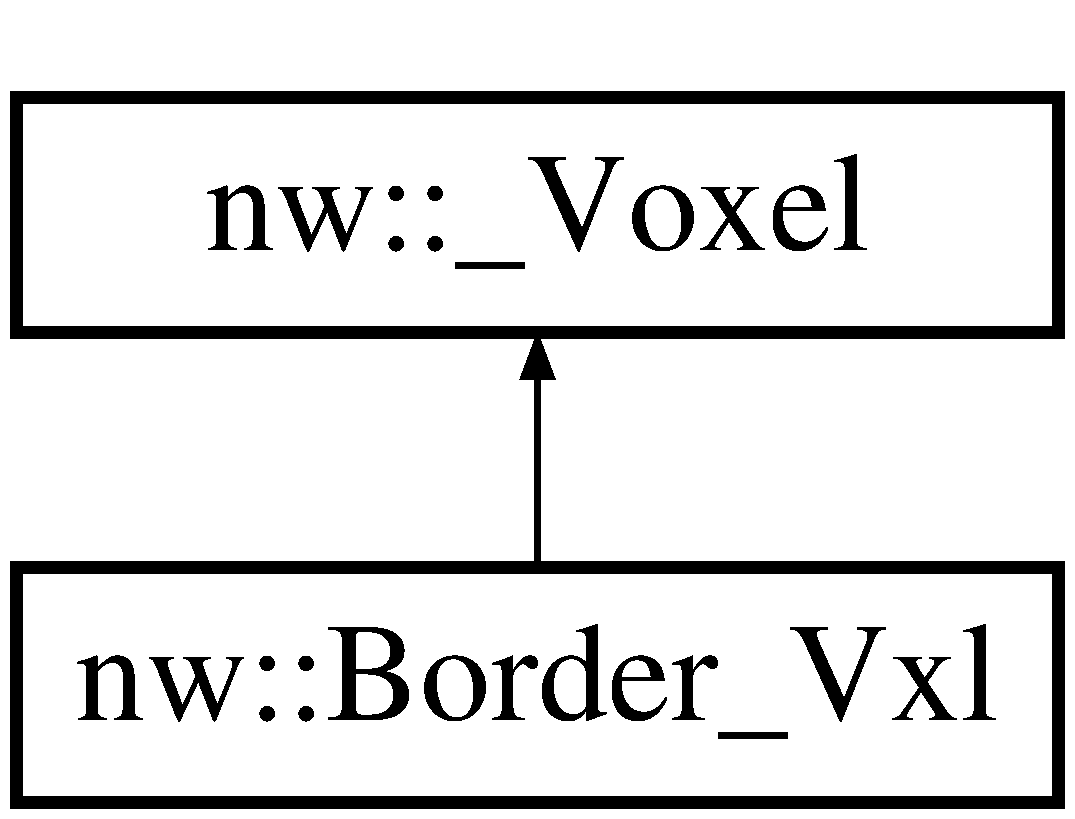
\includegraphics[height=2.000000cm]{d3/d72/classnw_1_1_border___vxl}
\end{center}
\end{figure}
\subsection*{Public Member Functions}
\begin{DoxyCompactItemize}
\item 
\hyperlink{classnw_1_1_border___vxl_a9fec31173af0a4b458af9670d274c7c9}{Border\+\_\+\+Vxl} (long \hyperlink{classnw_1_1___voxel_a01b73aff9af26230df4c483c5bd81896}{id}, double \hyperlink{classnw_1_1___voxel_ad9c3dbd0ea989af6ba7e1b5e09f6a989}{box\+\_\+length}, \hyperlink{namespacenw_a68aa8285591d78ebfc793c531bd43a23}{Species\+Vector} \hyperlink{classnw_1_1___voxel_a7762f59802c2a0b54bd18acbf803ff34}{state\+\_\+vec})
\begin{DoxyCompactList}\small\item\em Constructor. \end{DoxyCompactList}\item 
\hyperlink{classnw_1_1_border___vxl_a6874c3e65b625da883448d2c6811a0b7}{$\sim$\+Border\+\_\+\+Vxl} ()
\item 
void \hyperlink{classnw_1_1_border___vxl_aa7bd84871cf4a9781a535a0a1922dcc8}{update\+\_\+state} (std\+::vector$<$ long $>$ sc\+\_\+vec)
\begin{DoxyCompactList}\small\item\em Implementation of the \hyperlink{classnw_1_1___voxel_a5842ac3c24bda907204852db0cf46810}{\+\_\+\+Voxel\+::update\+\_\+state()} method. \end{DoxyCompactList}\end{DoxyCompactItemize}
\subsection*{Additional Inherited Members}


\subsection{Detailed Description}
Specialized \hyperlink{classnw_1_1___voxel}{\+\_\+\+Voxel} that can be used to define a system with equilibrium as boundary condition. 

The equilibrium boundary condition is an open system that is in equilibrium with itself and the surroundings. Border voxel serve as neighbor voxel for marginal voxel. Their state vector represents an equilibrium state of the considered system and exchanges non-\/stationary molecules with the main simulation voxels. The only exception is that the state of the border voxel is constant and thus drives the main simulation voxel towards the initial equilibrium. This plays an particular important role when conducting ion channels are introduced to the model. Without the eflux via border voxel, ions introduced via the channel would accumulate inside the main simulation voxel and thus disturb the relaxation of the system towards its equilibrium state. 

\subsection{Constructor \& Destructor Documentation}
\hypertarget{classnw_1_1_border___vxl_a9fec31173af0a4b458af9670d274c7c9}{\index{nw\+::\+Border\+\_\+\+Vxl@{nw\+::\+Border\+\_\+\+Vxl}!Border\+\_\+\+Vxl@{Border\+\_\+\+Vxl}}
\index{Border\+\_\+\+Vxl@{Border\+\_\+\+Vxl}!nw\+::\+Border\+\_\+\+Vxl@{nw\+::\+Border\+\_\+\+Vxl}}
\subsubsection[{Border\+\_\+\+Vxl}]{\setlength{\rightskip}{0pt plus 5cm}nw\+::\+Border\+\_\+\+Vxl\+::\+Border\+\_\+\+Vxl (
\begin{DoxyParamCaption}
\item[{long}]{id, }
\item[{double}]{box\+\_\+length, }
\item[{{\bf Species\+Vector}}]{state\+\_\+vec}
\end{DoxyParamCaption}
)\hspace{0.3cm}{\ttfamily [inline]}}}\label{classnw_1_1_border___vxl_a9fec31173af0a4b458af9670d274c7c9}


Constructor. 


\begin{DoxyParams}{Parameters}
{\em id} & \hyperlink{classnw_1_1___voxel}{\+\_\+\+Voxel} I\+D \\
\hline
{\em box\+\_\+length} & \hyperlink{classnw_1_1___voxel}{\+\_\+\+Voxel} box length \\
\hline
{\em state\+\_\+vec} & \hyperlink{classnw_1_1___voxel}{\+\_\+\+Voxel} state vector \\
\hline
\end{DoxyParams}

\begin{DoxyCode}
27                                                                     :
28         \hyperlink{classnw_1_1___voxel_a0622dd383528f5115c6a450b6cbb1b34}{\_Voxel}(\textcolor{keywordtype}{id}, \hyperlink{classnw_1_1___voxel_ad9c3dbd0ea989af6ba7e1b5e09f6a989}{box\_length}, \hyperlink{classnw_1_1___voxel_a7762f59802c2a0b54bd18acbf803ff34}{state\_vec}) \{\}
\end{DoxyCode}
\hypertarget{classnw_1_1_border___vxl_a6874c3e65b625da883448d2c6811a0b7}{\index{nw\+::\+Border\+\_\+\+Vxl@{nw\+::\+Border\+\_\+\+Vxl}!````~Border\+\_\+\+Vxl@{$\sim$\+Border\+\_\+\+Vxl}}
\index{````~Border\+\_\+\+Vxl@{$\sim$\+Border\+\_\+\+Vxl}!nw\+::\+Border\+\_\+\+Vxl@{nw\+::\+Border\+\_\+\+Vxl}}
\subsubsection[{$\sim$\+Border\+\_\+\+Vxl}]{\setlength{\rightskip}{0pt plus 5cm}nw\+::\+Border\+\_\+\+Vxl\+::$\sim$\+Border\+\_\+\+Vxl (
\begin{DoxyParamCaption}
{}
\end{DoxyParamCaption}
)\hspace{0.3cm}{\ttfamily [inline]}}}\label{classnw_1_1_border___vxl_a6874c3e65b625da883448d2c6811a0b7}
Destructor 
\begin{DoxyCode}
30 \{\}
\end{DoxyCode}


\subsection{Member Function Documentation}
\hypertarget{classnw_1_1_border___vxl_aa7bd84871cf4a9781a535a0a1922dcc8}{\index{nw\+::\+Border\+\_\+\+Vxl@{nw\+::\+Border\+\_\+\+Vxl}!update\+\_\+state@{update\+\_\+state}}
\index{update\+\_\+state@{update\+\_\+state}!nw\+::\+Border\+\_\+\+Vxl@{nw\+::\+Border\+\_\+\+Vxl}}
\subsubsection[{update\+\_\+state}]{\setlength{\rightskip}{0pt plus 5cm}void nw\+::\+Border\+\_\+\+Vxl\+::update\+\_\+state (
\begin{DoxyParamCaption}
\item[{std\+::vector$<$ long $>$}]{sc\+\_\+vec}
\end{DoxyParamCaption}
)}}\label{classnw_1_1_border___vxl_aa7bd84871cf4a9781a535a0a1922dcc8}


Implementation of the \hyperlink{classnw_1_1___voxel_a5842ac3c24bda907204852db0cf46810}{\+\_\+\+Voxel\+::update\+\_\+state()} method. 


\begin{DoxyParams}{Parameters}
{\em sc\+\_\+vec} & State change vector of firing event\\
\hline
\end{DoxyParams}
The state vector of the Border voxel is constant. This function thus does not alter the number of molecules. However, it does set respective dirty\+\_\+flags. 
\begin{DoxyCode}
7 \{
8     this->\hyperlink{classnw_1_1___voxel_a9c331fe7c0fd8691ef0124f33809764f}{dirty\_flag} = \textcolor{keyword}{true};
9 
10 \textcolor{comment}{//  do not update the state vector of Border\_vxl!}
11     \textcolor{keywordflow}{for} (\textcolor{keywordtype}{size\_t} i = 0; i < sc\_vec.size(); ++i) \{
12         \textcolor{keywordflow}{if} (sc\_vec[i] != 0) \{
13             \hyperlink{classnw_1_1___voxel_a7762f59802c2a0b54bd18acbf803ff34}{state\_vec}[i]->set\_dirty\_flag(\textcolor{keyword}{true});
14         \}
15     \}
16 \}
\end{DoxyCode}


The documentation for this class was generated from the following files\+:\begin{DoxyCompactItemize}
\item 
Voxel/\hyperlink{_border___vxl_8h}{Border\+\_\+\+Vxl.\+h}\item 
Voxel/\hyperlink{_border___vxl_8cpp}{Border\+\_\+\+Vxl.\+cpp}\end{DoxyCompactItemize}

\hypertarget{classnw_1_1_channel___spc}{\section{nw\+:\+:Channel\+\_\+\+Spc Class Reference}
\label{classnw_1_1_channel___spc}\index{nw\+::\+Channel\+\_\+\+Spc@{nw\+::\+Channel\+\_\+\+Spc}}
}


Realization of channel proteins comprised of a fixed number of subunits that open whenever a predefined number of those subunits are in an active state.  




{\ttfamily \#include $<$Channel\+\_\+\+Spc.\+h$>$}

Inheritance diagram for nw\+:\+:Channel\+\_\+\+Spc\+:\begin{figure}[H]
\begin{center}
\leavevmode
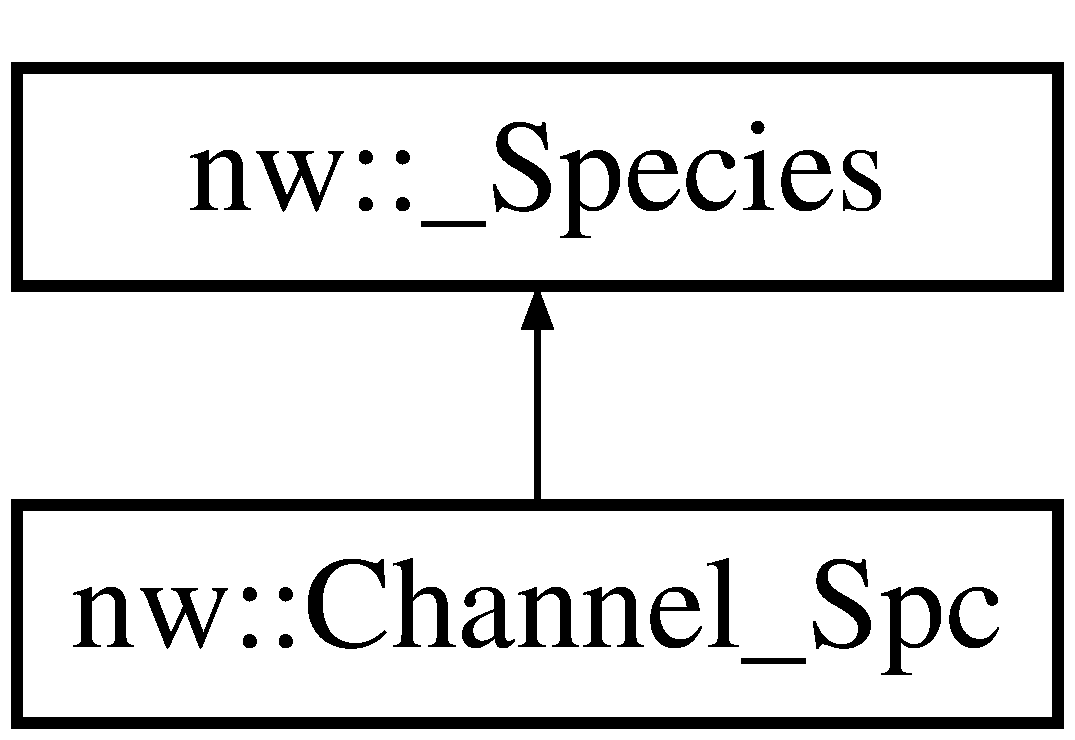
\includegraphics[height=2.000000cm]{db/dde/classnw_1_1_channel___spc}
\end{center}
\end{figure}
\subsection*{Public Member Functions}
\begin{DoxyCompactItemize}
\item 
\hyperlink{classnw_1_1_channel___spc_a050d0e4c96bc1ad37b259185e678b0b9}{Channel\+\_\+\+Spc} (long \hyperlink{classnw_1_1___species_ac42dfe1c656c17178a9649093519ebb7}{id}, string \hyperlink{classnw_1_1___species_a7b8ede09e28941beb48cf27f1247e2f9}{name}, double \hyperlink{classnw_1_1___species_ac66cdd3bdd5be88791e00d063b4e92a2}{initial\+\_\+conc}, int \hyperlink{classnw_1_1_channel___spc_a2b63ef7e5147046919cf96060b57e078}{n\+\_\+\+Subunits}, int \hyperlink{classnw_1_1_channel___spc_a52e6e8aae67ebfb6cec1b79e7f125542}{n\+\_\+\+Subunits\+\_\+\+To\+\_\+\+Open})
\begin{DoxyCompactList}\small\item\em Constructor of Channel Species. \end{DoxyCompactList}\item 
\hyperlink{classnw_1_1_channel___spc_a6bcdcda43c49d5223ccf9398c63f5170}{$\sim$\+Channel\+\_\+\+Spc} ()
\item 
long \hyperlink{classnw_1_1_channel___spc_a20a1e6dd089794ad0e1035635a1e3fe0}{get\+\_\+n\+\_\+molecules} ()
\begin{DoxyCompactList}\small\item\em Implementation of the \hyperlink{classnw_1_1___species_a6e3e68477663ff511d75fb24cf01cb9f}{\+\_\+\+Species\+::get\+\_\+n\+\_\+molecules()} method. \end{DoxyCompactList}\item 
void \hyperlink{classnw_1_1_channel___spc_a03347a88efec50ad3acd0ff4025ed23d}{mod\+\_\+n\+\_\+molecules} (long n)
\begin{DoxyCompactList}\small\item\em Implementation of the \hyperlink{classnw_1_1___species_ac7955c9fe040d8cae8f3cae4684ed96b}{\+\_\+\+Species\+::mod\+\_\+n\+\_\+molecules()} method. \end{DoxyCompactList}\item 
\hyperlink{classnw_1_1___species}{\+\_\+\+Species} $\ast$ \hyperlink{classnw_1_1_channel___spc_ab35f288a4021c302b4e2dc09e54578b1}{copy} ()
\begin{DoxyCompactList}\small\item\em Implementation of the \hyperlink{classnw_1_1___species_aea43d96b0b1c9e88953f40fbe58e7f29}{\+\_\+\+Species\+::copy()} method. \end{DoxyCompactList}\item 
void \hyperlink{classnw_1_1_channel___spc_af8d5d7097d343e6646c6c11a1744024d}{set\+\_\+n\+\_\+molecules} (double \hyperlink{classnw_1_1___species_a80896a55f086f468396e76ae8f1e8285}{volume})
\begin{DoxyCompactList}\small\item\em Implementation of the \hyperlink{classnw_1_1___species_a53d06cca549a83bfff71303174707926}{\+\_\+\+Species\+::set\+\_\+n\+\_\+molecules()} method. \end{DoxyCompactList}\item 
long \hyperlink{classnw_1_1_channel___spc_aecd939824b8d2a275cbe360f60ae4a2d}{get\+\_\+n\+\_\+\+Activable\+\_\+\+Ch} ()
\item 
long \hyperlink{classnw_1_1_channel___spc_a99c02ea4a145d6531ed2328de073fb37}{get\+\_\+n\+\_\+\+Inactivable\+\_\+\+Ch} ()
\item 
void \hyperlink{classnw_1_1_channel___spc_ab5176b0d9aed2ac68a142488d11b5e81}{activate\+\_\+\+Subunit} (long)
\begin{DoxyCompactList}\small\item\em Activates a subunit if the Sub\+Unit\+Switch Reaction Event increases the number of active subunits. \end{DoxyCompactList}\item 
void \hyperlink{classnw_1_1_channel___spc_a190172435ab84f9210ae027d06aae81a}{inactivate\+\_\+\+Subunit} (long)
\begin{DoxyCompactList}\small\item\em Inactivates a subunit if the Sub\+Unit\+Switch Reaction Event decreases the number of active subunits. \end{DoxyCompactList}\end{DoxyCompactItemize}
\subsection*{Private Attributes}
\begin{DoxyCompactItemize}
\item 
int \hyperlink{classnw_1_1_channel___spc_a2b63ef7e5147046919cf96060b57e078}{n\+\_\+\+Subunits}
\begin{DoxyCompactList}\small\item\em Number of subunits of this channel species. \end{DoxyCompactList}\item 
int \hyperlink{classnw_1_1_channel___spc_a52e6e8aae67ebfb6cec1b79e7f125542}{n\+\_\+\+Subunits\+\_\+\+To\+\_\+\+Open}
\begin{DoxyCompactList}\small\item\em Number of activated subunits that are required to open the channel. \end{DoxyCompactList}\item 
long \hyperlink{classnw_1_1_channel___spc_a67fd1b83563c30ec86802bdab420c95d}{n\+\_\+active\+\_\+\+Ch}
\begin{DoxyCompactList}\small\item\em Number of currently active channels. \end{DoxyCompactList}\item 
long \hyperlink{classnw_1_1_channel___spc_ac6ae04b799c751bb61918b4ab163ce85}{n\+\_\+fully\+\_\+activated\+\_\+\+Ch}
\begin{DoxyCompactList}\small\item\em Number of completely activated channels (no subunit activation possible). \end{DoxyCompactList}\item 
long \hyperlink{classnw_1_1_channel___spc_a35afc71aa0eeb5b1e4a2089a5c1f65ae}{n\+\_\+fully\+\_\+inactivated\+\_\+\+Ch}
\begin{DoxyCompactList}\small\item\em Number of completely inactivated channels (no subunit inactivation possible) \end{DoxyCompactList}\item 
vector$<$ long $>$ \hyperlink{classnw_1_1_channel___spc_aca3ddf4eba759eeeb835bba168795a11}{ch\+\_\+\+Vec}
\begin{DoxyCompactList}\small\item\em Vector representing the number of active subunits of each channel. \end{DoxyCompactList}\item 
vector$<$ long $>$\+::iterator \hyperlink{classnw_1_1_channel___spc_a025013604067ea03dce585fb5a785408}{ch\+\_\+it}
\begin{DoxyCompactList}\small\item\em Vector iterator that iterates through the channel vector to update it. \end{DoxyCompactList}\end{DoxyCompactItemize}
\subsection*{Additional Inherited Members}


\subsection{Detailed Description}
Realization of channel proteins comprised of a fixed number of subunits that open whenever a predefined number of those subunits are in an active state. 

This species works a little different from others. It is an "imaginary" \hyperlink{classnw_1_1___species}{\+\_\+\+Species}. It only subsumes a certain number of other Species (here subunits). The molecular count only changes if there are enough active subunits. A channel only exists in this implementation if it is open. To keep track of active subunits, there is an event called subunit switch reaction that defines the transition between an inactive and an active subunit. If this event occurs it typecasts the Species at the channel species id (class attribute to be defined in the input file\+: ch\+\_\+spc\+\_\+id) to a channel species and calls activate\+\_\+subunit() resp. inactivate\+\_\+subunit(). ~\newline
~\newline
Note\+: To avoid the typcast which can cause instabilities, it might be benifical to extend the existing framework with an event handling system. 

\subsection{Constructor \& Destructor Documentation}
\hypertarget{classnw_1_1_channel___spc_a050d0e4c96bc1ad37b259185e678b0b9}{\index{nw\+::\+Channel\+\_\+\+Spc@{nw\+::\+Channel\+\_\+\+Spc}!Channel\+\_\+\+Spc@{Channel\+\_\+\+Spc}}
\index{Channel\+\_\+\+Spc@{Channel\+\_\+\+Spc}!nw\+::\+Channel\+\_\+\+Spc@{nw\+::\+Channel\+\_\+\+Spc}}
\subsubsection[{Channel\+\_\+\+Spc}]{\setlength{\rightskip}{0pt plus 5cm}nw\+::\+Channel\+\_\+\+Spc\+::\+Channel\+\_\+\+Spc (
\begin{DoxyParamCaption}
\item[{long}]{id, }
\item[{string}]{name, }
\item[{double}]{initial\+\_\+conc, }
\item[{int}]{n\+\_\+\+Subunits, }
\item[{int}]{n\+\_\+\+Subunits\+\_\+\+To\+\_\+\+Open}
\end{DoxyParamCaption}
)\hspace{0.3cm}{\ttfamily [inline]}}}\label{classnw_1_1_channel___spc_a050d0e4c96bc1ad37b259185e678b0b9}


Constructor of Channel Species. 


\begin{DoxyParams}{Parameters}
{\em id} & \hyperlink{classnw_1_1___species}{\+\_\+\+Species} I\+D \\
\hline
{\em name} & \hyperlink{classnw_1_1___species}{\+\_\+\+Species} name \\
\hline
{\em initial\+\_\+conc} & \hyperlink{classnw_1_1___species}{\+\_\+\+Species} initial concentration \\
\hline
{\em n\+\_\+\+Subunits} & Number of existing subunits the channel is build of. \\
\hline
{\em n\+\_\+\+Subunits\+\_\+\+To\+\_\+\+Open} & Required number of active subunits to open the channel \\
\hline
\end{DoxyParams}

\begin{DoxyCode}
35                                                                                                   :
36         \hyperlink{classnw_1_1___species_af74ef3f4a59f3c8fa9ff6b1acc83be86}{\_Species}(\textcolor{keywordtype}{id},\hyperlink{classnw_1_1___species_a7b8ede09e28941beb48cf27f1247e2f9}{name},\hyperlink{classnw_1_1___species_ac66cdd3bdd5be88791e00d063b4e92a2}{initial\_conc}),
37         \hyperlink{classnw_1_1_channel___spc_a2b63ef7e5147046919cf96060b57e078}{n\_Subunits}(\hyperlink{classnw_1_1_channel___spc_a2b63ef7e5147046919cf96060b57e078}{n\_Subunits}),
38         \hyperlink{classnw_1_1_channel___spc_a52e6e8aae67ebfb6cec1b79e7f125542}{n\_Subunits\_To\_Open}(\hyperlink{classnw_1_1_channel___spc_a52e6e8aae67ebfb6cec1b79e7f125542}{n\_Subunits\_To\_Open}),
39         \hyperlink{classnw_1_1_channel___spc_a67fd1b83563c30ec86802bdab420c95d}{n\_active\_Ch}(0),
40         \hyperlink{classnw_1_1_channel___spc_ac6ae04b799c751bb61918b4ab163ce85}{n\_fully\_activated\_Ch}(0),
41         \hyperlink{classnw_1_1_channel___spc_a35afc71aa0eeb5b1e4a2089a5c1f65ae}{n\_fully\_inactivated\_Ch}(0)\{\}
\end{DoxyCode}
\hypertarget{classnw_1_1_channel___spc_a6bcdcda43c49d5223ccf9398c63f5170}{\index{nw\+::\+Channel\+\_\+\+Spc@{nw\+::\+Channel\+\_\+\+Spc}!````~Channel\+\_\+\+Spc@{$\sim$\+Channel\+\_\+\+Spc}}
\index{````~Channel\+\_\+\+Spc@{$\sim$\+Channel\+\_\+\+Spc}!nw\+::\+Channel\+\_\+\+Spc@{nw\+::\+Channel\+\_\+\+Spc}}
\subsubsection[{$\sim$\+Channel\+\_\+\+Spc}]{\setlength{\rightskip}{0pt plus 5cm}nw\+::\+Channel\+\_\+\+Spc\+::$\sim$\+Channel\+\_\+\+Spc (
\begin{DoxyParamCaption}
{}
\end{DoxyParamCaption}
)\hspace{0.3cm}{\ttfamily [inline]}}}\label{classnw_1_1_channel___spc_a6bcdcda43c49d5223ccf9398c63f5170}
Destructor 
\begin{DoxyCode}
43 \{\};
\end{DoxyCode}


\subsection{Member Function Documentation}
\hypertarget{classnw_1_1_channel___spc_ab5176b0d9aed2ac68a142488d11b5e81}{\index{nw\+::\+Channel\+\_\+\+Spc@{nw\+::\+Channel\+\_\+\+Spc}!activate\+\_\+\+Subunit@{activate\+\_\+\+Subunit}}
\index{activate\+\_\+\+Subunit@{activate\+\_\+\+Subunit}!nw\+::\+Channel\+\_\+\+Spc@{nw\+::\+Channel\+\_\+\+Spc}}
\subsubsection[{activate\+\_\+\+Subunit}]{\setlength{\rightskip}{0pt plus 5cm}void nw\+::\+Channel\+\_\+\+Spc\+::activate\+\_\+\+Subunit (
\begin{DoxyParamCaption}
\item[{long}]{rnd\+\_\+id}
\end{DoxyParamCaption}
)}}\label{classnw_1_1_channel___spc_ab5176b0d9aed2ac68a142488d11b5e81}


Activates a subunit if the Sub\+Unit\+Switch Reaction Event increases the number of active subunits. 


\begin{DoxyParams}{Parameters}
{\em rnd\+\_\+id} & Random number to pick a channel whose subunit will be activated.\\
\hline
\end{DoxyParams}
If a subunit is activated, first of all a random number has to be generated (see Sub\+Unit\+Switch\+\_\+\+Rct\+\_\+evt) to pick one of the existing channels whose subunit is activated.~\newline
~\newline
Note\+: It is not possible to increase the number of active channel subunits if all subunits are in the active state. This makes this function a little bit more complex. 
\begin{DoxyCode}
6                                              \{
7     \hyperlink{classnw_1_1_channel___spc_a025013604067ea03dce585fb5a785408}{ch\_it} = \hyperlink{classnw_1_1_channel___spc_aca3ddf4eba759eeeb835bba168795a11}{ch\_Vec}.begin();
8 
9 \textcolor{comment}{//  iterate to an activatable channel}
10     \textcolor{keywordflow}{for} (\textcolor{keywordtype}{size\_t} i = 0; i <= size\_t(rnd\_id);++i)\{
11         \textcolor{keywordflow}{if}(i!=0)\{\hyperlink{classnw_1_1_channel___spc_a025013604067ea03dce585fb5a785408}{ch\_it}++;\}
12         \textcolor{keywordflow}{while}(*\hyperlink{classnw_1_1_channel___spc_a025013604067ea03dce585fb5a785408}{ch\_it} == \hyperlink{classnw_1_1_channel___spc_a2b63ef7e5147046919cf96060b57e078}{n\_Subunits})\{
13             \hyperlink{classnw_1_1_channel___spc_a025013604067ea03dce585fb5a785408}{ch\_it}++;
14         \}
15     \}
16 
17 \textcolor{comment}{//  decrease number of completely inactivated Channel if it was a Channel with 0 active subunits}
18     \textcolor{keywordflow}{if}(*\hyperlink{classnw_1_1_channel___spc_a025013604067ea03dce585fb5a785408}{ch\_it} == 0)\{\hyperlink{classnw_1_1_channel___spc_a35afc71aa0eeb5b1e4a2089a5c1f65ae}{n\_fully\_inactivated\_Ch}--; 
      \hyperlink{classnw_1_1___species_a79157bae3920ce7bba35e3f75b2aad6f}{dirty\_flag} = \textcolor{keyword}{true};\}
19 \textcolor{comment}{//  increase number of active subunits and check if the channel is open!}
20     \textcolor{keywordflow}{if}(++*\hyperlink{classnw_1_1_channel___spc_a025013604067ea03dce585fb5a785408}{ch\_it} == \hyperlink{classnw_1_1_channel___spc_a52e6e8aae67ebfb6cec1b79e7f125542}{n\_Subunits\_To\_Open})\{\hyperlink{classnw_1_1_channel___spc_a67fd1b83563c30ec86802bdab420c95d}{n\_active\_Ch}++; 
      \hyperlink{classnw_1_1___species_a79157bae3920ce7bba35e3f75b2aad6f}{dirty\_flag} = \textcolor{keyword}{true};\}
21 \textcolor{comment}{//  if the channel is completely activated, increase number of fully activated channels}
22     \textcolor{keywordflow}{if} (*\hyperlink{classnw_1_1_channel___spc_a025013604067ea03dce585fb5a785408}{ch\_it} == \hyperlink{classnw_1_1_channel___spc_a2b63ef7e5147046919cf96060b57e078}{n\_Subunits}) \{\hyperlink{classnw_1_1_channel___spc_ac6ae04b799c751bb61918b4ab163ce85}{n\_fully\_activated\_Ch}++; 
      \hyperlink{classnw_1_1___species_a79157bae3920ce7bba35e3f75b2aad6f}{dirty\_flag} = \textcolor{keyword}{true};\}
23 \}
\end{DoxyCode}
\hypertarget{classnw_1_1_channel___spc_ab35f288a4021c302b4e2dc09e54578b1}{\index{nw\+::\+Channel\+\_\+\+Spc@{nw\+::\+Channel\+\_\+\+Spc}!copy@{copy}}
\index{copy@{copy}!nw\+::\+Channel\+\_\+\+Spc@{nw\+::\+Channel\+\_\+\+Spc}}
\subsubsection[{copy}]{\setlength{\rightskip}{0pt plus 5cm}{\bf \+\_\+\+Species}$\ast$ nw\+::\+Channel\+\_\+\+Spc\+::copy (
\begin{DoxyParamCaption}
{}
\end{DoxyParamCaption}
)\hspace{0.3cm}{\ttfamily [inline]}, {\ttfamily [virtual]}}}\label{classnw_1_1_channel___spc_ab35f288a4021c302b4e2dc09e54578b1}


Implementation of the \hyperlink{classnw_1_1___species_aea43d96b0b1c9e88953f40fbe58e7f29}{\+\_\+\+Species\+::copy()} method. 



Implements \hyperlink{classnw_1_1___species_aea43d96b0b1c9e88953f40fbe58e7f29}{nw\+::\+\_\+\+Species}.


\begin{DoxyCode}
57                     \{
58         \hyperlink{classnw_1_1___species_af74ef3f4a59f3c8fa9ff6b1acc83be86}{\_Species}* s = \textcolor{keyword}{new} \hyperlink{classnw_1_1_channel___spc_a050d0e4c96bc1ad37b259185e678b0b9}{Channel\_Spc}(\textcolor{keywordtype}{id},\hyperlink{classnw_1_1___species_a7b8ede09e28941beb48cf27f1247e2f9}{name},
      \hyperlink{classnw_1_1___species_ac66cdd3bdd5be88791e00d063b4e92a2}{initial\_conc},\hyperlink{classnw_1_1_channel___spc_a2b63ef7e5147046919cf96060b57e078}{n\_Subunits},\hyperlink{classnw_1_1_channel___spc_a52e6e8aae67ebfb6cec1b79e7f125542}{n\_Subunits\_To\_Open});
59         \textcolor{keywordflow}{return} s;\}
\end{DoxyCode}
\hypertarget{classnw_1_1_channel___spc_aecd939824b8d2a275cbe360f60ae4a2d}{\index{nw\+::\+Channel\+\_\+\+Spc@{nw\+::\+Channel\+\_\+\+Spc}!get\+\_\+n\+\_\+\+Activable\+\_\+\+Ch@{get\+\_\+n\+\_\+\+Activable\+\_\+\+Ch}}
\index{get\+\_\+n\+\_\+\+Activable\+\_\+\+Ch@{get\+\_\+n\+\_\+\+Activable\+\_\+\+Ch}!nw\+::\+Channel\+\_\+\+Spc@{nw\+::\+Channel\+\_\+\+Spc}}
\subsubsection[{get\+\_\+n\+\_\+\+Activable\+\_\+\+Ch}]{\setlength{\rightskip}{0pt plus 5cm}long nw\+::\+Channel\+\_\+\+Spc\+::get\+\_\+n\+\_\+\+Activable\+\_\+\+Ch (
\begin{DoxyParamCaption}
{}
\end{DoxyParamCaption}
)\hspace{0.3cm}{\ttfamily [inline]}}}\label{classnw_1_1_channel___spc_aecd939824b8d2a275cbe360f60ae4a2d}

\begin{DoxyCode}
73 \{\textcolor{keywordflow}{return} \hyperlink{classnw_1_1___species_af6ae0232b4f994b464a2f69cb022b33f}{n\_molecules} - \hyperlink{classnw_1_1_channel___spc_ac6ae04b799c751bb61918b4ab163ce85}{n\_fully\_activated\_Ch};\}
\end{DoxyCode}
\hypertarget{classnw_1_1_channel___spc_a99c02ea4a145d6531ed2328de073fb37}{\index{nw\+::\+Channel\+\_\+\+Spc@{nw\+::\+Channel\+\_\+\+Spc}!get\+\_\+n\+\_\+\+Inactivable\+\_\+\+Ch@{get\+\_\+n\+\_\+\+Inactivable\+\_\+\+Ch}}
\index{get\+\_\+n\+\_\+\+Inactivable\+\_\+\+Ch@{get\+\_\+n\+\_\+\+Inactivable\+\_\+\+Ch}!nw\+::\+Channel\+\_\+\+Spc@{nw\+::\+Channel\+\_\+\+Spc}}
\subsubsection[{get\+\_\+n\+\_\+\+Inactivable\+\_\+\+Ch}]{\setlength{\rightskip}{0pt plus 5cm}long nw\+::\+Channel\+\_\+\+Spc\+::get\+\_\+n\+\_\+\+Inactivable\+\_\+\+Ch (
\begin{DoxyParamCaption}
{}
\end{DoxyParamCaption}
)\hspace{0.3cm}{\ttfamily [inline]}}}\label{classnw_1_1_channel___spc_a99c02ea4a145d6531ed2328de073fb37}

\begin{DoxyCode}
74 \{\textcolor{keywordflow}{return} \hyperlink{classnw_1_1___species_af6ae0232b4f994b464a2f69cb022b33f}{n\_molecules} - \hyperlink{classnw_1_1_channel___spc_a35afc71aa0eeb5b1e4a2089a5c1f65ae}{n\_fully\_inactivated\_Ch};\}
\end{DoxyCode}
\hypertarget{classnw_1_1_channel___spc_a20a1e6dd089794ad0e1035635a1e3fe0}{\index{nw\+::\+Channel\+\_\+\+Spc@{nw\+::\+Channel\+\_\+\+Spc}!get\+\_\+n\+\_\+molecules@{get\+\_\+n\+\_\+molecules}}
\index{get\+\_\+n\+\_\+molecules@{get\+\_\+n\+\_\+molecules}!nw\+::\+Channel\+\_\+\+Spc@{nw\+::\+Channel\+\_\+\+Spc}}
\subsubsection[{get\+\_\+n\+\_\+molecules}]{\setlength{\rightskip}{0pt plus 5cm}long nw\+::\+Channel\+\_\+\+Spc\+::get\+\_\+n\+\_\+molecules (
\begin{DoxyParamCaption}
{}
\end{DoxyParamCaption}
)\hspace{0.3cm}{\ttfamily [inline]}, {\ttfamily [virtual]}}}\label{classnw_1_1_channel___spc_a20a1e6dd089794ad0e1035635a1e3fe0}


Implementation of the \hyperlink{classnw_1_1___species_a6e3e68477663ff511d75fb24cf01cb9f}{\+\_\+\+Species\+::get\+\_\+n\+\_\+molecules()} method. 

\begin{DoxyReturn}{Returns}
Number of open channel.
\end{DoxyReturn}
Only the number of open channels are returned. The total number of channels includes closed non-\/conducting channels. 

Implements \hyperlink{classnw_1_1___species_a6e3e68477663ff511d75fb24cf01cb9f}{nw\+::\+\_\+\+Species}.


\begin{DoxyCode}
49 \{\textcolor{keywordflow}{return} \hyperlink{classnw_1_1_channel___spc_a67fd1b83563c30ec86802bdab420c95d}{n\_active\_Ch};\}
\end{DoxyCode}
\hypertarget{classnw_1_1_channel___spc_a190172435ab84f9210ae027d06aae81a}{\index{nw\+::\+Channel\+\_\+\+Spc@{nw\+::\+Channel\+\_\+\+Spc}!inactivate\+\_\+\+Subunit@{inactivate\+\_\+\+Subunit}}
\index{inactivate\+\_\+\+Subunit@{inactivate\+\_\+\+Subunit}!nw\+::\+Channel\+\_\+\+Spc@{nw\+::\+Channel\+\_\+\+Spc}}
\subsubsection[{inactivate\+\_\+\+Subunit}]{\setlength{\rightskip}{0pt plus 5cm}void nw\+::\+Channel\+\_\+\+Spc\+::inactivate\+\_\+\+Subunit (
\begin{DoxyParamCaption}
\item[{long}]{rnd\+\_\+id}
\end{DoxyParamCaption}
)}}\label{classnw_1_1_channel___spc_a190172435ab84f9210ae027d06aae81a}


Inactivates a subunit if the Sub\+Unit\+Switch Reaction Event decreases the number of active subunits. 


\begin{DoxyParams}{Parameters}
{\em rnd\+\_\+id} & random number to pick a channel whose subunit will be inactivated.\\
\hline
\end{DoxyParams}
If a subunit is inactivated, first of all a random number has to be generated (see Sub\+Unit\+Switch\+\_\+\+Rct\+\_\+evt) to pick one of the existing channels whose subunit is inactivated.~\newline
~\newline
Note\+: It is not possible to decrease the number of active channel subunits if all subunits are inactivated. This makes this function a little bit more complex. 
\begin{DoxyCode}
25                                                \{
26     \hyperlink{classnw_1_1_channel___spc_a025013604067ea03dce585fb5a785408}{ch\_it} = \hyperlink{classnw_1_1_channel___spc_aca3ddf4eba759eeeb835bba168795a11}{ch\_Vec}.begin();
27 \textcolor{comment}{//  iterate to an inactivatable channel}
28     \textcolor{keywordflow}{for} (\textcolor{keywordtype}{size\_t} i = 0; i <= (size\_t)rnd\_id;++i)\{
29         \textcolor{keywordflow}{if}(i!=0)\{\hyperlink{classnw_1_1_channel___spc_a025013604067ea03dce585fb5a785408}{ch\_it}++;\}
30         \textcolor{keywordflow}{while}(*\hyperlink{classnw_1_1_channel___spc_a025013604067ea03dce585fb5a785408}{ch\_it} == 0)\{
31             \hyperlink{classnw_1_1_channel___spc_a025013604067ea03dce585fb5a785408}{ch\_it}++;
32         \}
33     \}
34 
35 \textcolor{comment}{//  decrease number of fully activated Channel if it was a Channel with maximum active subunits}
36     \textcolor{keywordflow}{if}(*\hyperlink{classnw_1_1_channel___spc_a025013604067ea03dce585fb5a785408}{ch\_it} == \hyperlink{classnw_1_1_channel___spc_a2b63ef7e5147046919cf96060b57e078}{n\_Subunits})\{\hyperlink{classnw_1_1_channel___spc_ac6ae04b799c751bb61918b4ab163ce85}{n\_fully\_activated\_Ch}--; 
      \hyperlink{classnw_1_1___species_a79157bae3920ce7bba35e3f75b2aad6f}{dirty\_flag} = \textcolor{keyword}{true};\}
37 \textcolor{comment}{//  decrease number of active subunits and check if the channel is open!}
38     \textcolor{keywordflow}{if}(*\hyperlink{classnw_1_1_channel___spc_a025013604067ea03dce585fb5a785408}{ch\_it} == \hyperlink{classnw_1_1_channel___spc_a52e6e8aae67ebfb6cec1b79e7f125542}{n\_Subunits\_To\_Open})\{\hyperlink{classnw_1_1_channel___spc_a67fd1b83563c30ec86802bdab420c95d}{n\_active\_Ch}--; 
      \hyperlink{classnw_1_1___species_a79157bae3920ce7bba35e3f75b2aad6f}{dirty\_flag} = \textcolor{keyword}{true};\}
39 \textcolor{comment}{//  if the channel is completely inactivated, increase number of fully inactivated channels}
40     \textcolor{keywordflow}{if} (--*\hyperlink{classnw_1_1_channel___spc_a025013604067ea03dce585fb5a785408}{ch\_it} == 0) \{\hyperlink{classnw_1_1_channel___spc_a35afc71aa0eeb5b1e4a2089a5c1f65ae}{n\_fully\_inactivated\_Ch}++; 
      \hyperlink{classnw_1_1___species_a79157bae3920ce7bba35e3f75b2aad6f}{dirty\_flag} = \textcolor{keyword}{true};\}
41 \}
\end{DoxyCode}
\hypertarget{classnw_1_1_channel___spc_a03347a88efec50ad3acd0ff4025ed23d}{\index{nw\+::\+Channel\+\_\+\+Spc@{nw\+::\+Channel\+\_\+\+Spc}!mod\+\_\+n\+\_\+molecules@{mod\+\_\+n\+\_\+molecules}}
\index{mod\+\_\+n\+\_\+molecules@{mod\+\_\+n\+\_\+molecules}!nw\+::\+Channel\+\_\+\+Spc@{nw\+::\+Channel\+\_\+\+Spc}}
\subsubsection[{mod\+\_\+n\+\_\+molecules}]{\setlength{\rightskip}{0pt plus 5cm}void nw\+::\+Channel\+\_\+\+Spc\+::mod\+\_\+n\+\_\+molecules (
\begin{DoxyParamCaption}
\item[{long}]{n}
\end{DoxyParamCaption}
)\hspace{0.3cm}{\ttfamily [inline]}, {\ttfamily [virtual]}}}\label{classnw_1_1_channel___spc_a03347a88efec50ad3acd0ff4025ed23d}


Implementation of the \hyperlink{classnw_1_1___species_ac7955c9fe040d8cae8f3cae4684ed96b}{\+\_\+\+Species\+::mod\+\_\+n\+\_\+molecules()} method. 


\begin{DoxyParams}{Parameters}
{\em n} & Summand that is added to the current number of molecules.\\
\hline
\end{DoxyParams}
This function is empty, because at the moment there is no way how the number of channels could be modified but through the subunitswitch reaction which calls \hyperlink{classnw_1_1_channel___spc_ab5176b0d9aed2ac68a142488d11b5e81}{activate\+\_\+\+Subunit()} resp. \hyperlink{classnw_1_1_channel___spc_a190172435ab84f9210ae027d06aae81a}{inactivate\+\_\+\+Subunit()} 

Implements \hyperlink{classnw_1_1___species_ac7955c9fe040d8cae8f3cae4684ed96b}{nw\+::\+\_\+\+Species}.


\begin{DoxyCode}
55 \{\}
\end{DoxyCode}
\hypertarget{classnw_1_1_channel___spc_af8d5d7097d343e6646c6c11a1744024d}{\index{nw\+::\+Channel\+\_\+\+Spc@{nw\+::\+Channel\+\_\+\+Spc}!set\+\_\+n\+\_\+molecules@{set\+\_\+n\+\_\+molecules}}
\index{set\+\_\+n\+\_\+molecules@{set\+\_\+n\+\_\+molecules}!nw\+::\+Channel\+\_\+\+Spc@{nw\+::\+Channel\+\_\+\+Spc}}
\subsubsection[{set\+\_\+n\+\_\+molecules}]{\setlength{\rightskip}{0pt plus 5cm}void nw\+::\+Channel\+\_\+\+Spc\+::set\+\_\+n\+\_\+molecules (
\begin{DoxyParamCaption}
\item[{double}]{volume}
\end{DoxyParamCaption}
)\hspace{0.3cm}{\ttfamily [inline]}, {\ttfamily [virtual]}}}\label{classnw_1_1_channel___spc_af8d5d7097d343e6646c6c11a1744024d}


Implementation of the \hyperlink{classnw_1_1___species_a53d06cca549a83bfff71303174707926}{\+\_\+\+Species\+::set\+\_\+n\+\_\+molecules()} method. 

Initialization of the channel species. A vector with a length equal to the number of existing channels is created. Each element of this vector holds the number of active subunits for one particular channel protein. If the number of active subunits inside one vector field becomes equal or bigger than the number of subunits required to open a channel, the number of activated channel is increased by one. All channel are initially closed. 

Reimplemented from \hyperlink{classnw_1_1___species_a53d06cca549a83bfff71303174707926}{nw\+::\+\_\+\+Species}.


\begin{DoxyCode}
67                                        \{
68     \hyperlink{classnw_1_1___species_af6ae0232b4f994b464a2f69cb022b33f}{n\_molecules} = \hyperlink{classnw_1_1___species_a80896a55f086f468396e76ae8f1e8285}{volume}*1e-6*\hyperlink{namespacenw_ad890cfa7dd9eaf8d5b6754723e516c4a}{N\_AVO}*\hyperlink{classnw_1_1___species_ac66cdd3bdd5be88791e00d063b4e92a2}{initial\_conc};
69     \hyperlink{classnw_1_1_channel___spc_aca3ddf4eba759eeeb835bba168795a11}{ch\_Vec}.assign(\hyperlink{classnw_1_1___species_af6ae0232b4f994b464a2f69cb022b33f}{n\_molecules},0);
70     this->\hyperlink{classnw_1_1_channel___spc_a35afc71aa0eeb5b1e4a2089a5c1f65ae}{n\_fully\_inactivated\_Ch} = \hyperlink{classnw_1_1___species_af6ae0232b4f994b464a2f69cb022b33f}{n\_molecules};\}
\end{DoxyCode}


\subsection{Member Data Documentation}
\hypertarget{classnw_1_1_channel___spc_a025013604067ea03dce585fb5a785408}{\index{nw\+::\+Channel\+\_\+\+Spc@{nw\+::\+Channel\+\_\+\+Spc}!ch\+\_\+it@{ch\+\_\+it}}
\index{ch\+\_\+it@{ch\+\_\+it}!nw\+::\+Channel\+\_\+\+Spc@{nw\+::\+Channel\+\_\+\+Spc}}
\subsubsection[{ch\+\_\+it}]{\setlength{\rightskip}{0pt plus 5cm}vector$<$long$>$\+::iterator nw\+::\+Channel\+\_\+\+Spc\+::ch\+\_\+it\hspace{0.3cm}{\ttfamily [private]}}}\label{classnw_1_1_channel___spc_a025013604067ea03dce585fb5a785408}


Vector iterator that iterates through the channel vector to update it. 

\hypertarget{classnw_1_1_channel___spc_aca3ddf4eba759eeeb835bba168795a11}{\index{nw\+::\+Channel\+\_\+\+Spc@{nw\+::\+Channel\+\_\+\+Spc}!ch\+\_\+\+Vec@{ch\+\_\+\+Vec}}
\index{ch\+\_\+\+Vec@{ch\+\_\+\+Vec}!nw\+::\+Channel\+\_\+\+Spc@{nw\+::\+Channel\+\_\+\+Spc}}
\subsubsection[{ch\+\_\+\+Vec}]{\setlength{\rightskip}{0pt plus 5cm}vector$<$long$>$ nw\+::\+Channel\+\_\+\+Spc\+::ch\+\_\+\+Vec\hspace{0.3cm}{\ttfamily [private]}}}\label{classnw_1_1_channel___spc_aca3ddf4eba759eeeb835bba168795a11}


Vector representing the number of active subunits of each channel. 

\hypertarget{classnw_1_1_channel___spc_a67fd1b83563c30ec86802bdab420c95d}{\index{nw\+::\+Channel\+\_\+\+Spc@{nw\+::\+Channel\+\_\+\+Spc}!n\+\_\+active\+\_\+\+Ch@{n\+\_\+active\+\_\+\+Ch}}
\index{n\+\_\+active\+\_\+\+Ch@{n\+\_\+active\+\_\+\+Ch}!nw\+::\+Channel\+\_\+\+Spc@{nw\+::\+Channel\+\_\+\+Spc}}
\subsubsection[{n\+\_\+active\+\_\+\+Ch}]{\setlength{\rightskip}{0pt plus 5cm}long nw\+::\+Channel\+\_\+\+Spc\+::n\+\_\+active\+\_\+\+Ch\hspace{0.3cm}{\ttfamily [private]}}}\label{classnw_1_1_channel___spc_a67fd1b83563c30ec86802bdab420c95d}


Number of currently active channels. 

\hypertarget{classnw_1_1_channel___spc_ac6ae04b799c751bb61918b4ab163ce85}{\index{nw\+::\+Channel\+\_\+\+Spc@{nw\+::\+Channel\+\_\+\+Spc}!n\+\_\+fully\+\_\+activated\+\_\+\+Ch@{n\+\_\+fully\+\_\+activated\+\_\+\+Ch}}
\index{n\+\_\+fully\+\_\+activated\+\_\+\+Ch@{n\+\_\+fully\+\_\+activated\+\_\+\+Ch}!nw\+::\+Channel\+\_\+\+Spc@{nw\+::\+Channel\+\_\+\+Spc}}
\subsubsection[{n\+\_\+fully\+\_\+activated\+\_\+\+Ch}]{\setlength{\rightskip}{0pt plus 5cm}long nw\+::\+Channel\+\_\+\+Spc\+::n\+\_\+fully\+\_\+activated\+\_\+\+Ch\hspace{0.3cm}{\ttfamily [private]}}}\label{classnw_1_1_channel___spc_ac6ae04b799c751bb61918b4ab163ce85}


Number of completely activated channels (no subunit activation possible). 

\hypertarget{classnw_1_1_channel___spc_a35afc71aa0eeb5b1e4a2089a5c1f65ae}{\index{nw\+::\+Channel\+\_\+\+Spc@{nw\+::\+Channel\+\_\+\+Spc}!n\+\_\+fully\+\_\+inactivated\+\_\+\+Ch@{n\+\_\+fully\+\_\+inactivated\+\_\+\+Ch}}
\index{n\+\_\+fully\+\_\+inactivated\+\_\+\+Ch@{n\+\_\+fully\+\_\+inactivated\+\_\+\+Ch}!nw\+::\+Channel\+\_\+\+Spc@{nw\+::\+Channel\+\_\+\+Spc}}
\subsubsection[{n\+\_\+fully\+\_\+inactivated\+\_\+\+Ch}]{\setlength{\rightskip}{0pt plus 5cm}long nw\+::\+Channel\+\_\+\+Spc\+::n\+\_\+fully\+\_\+inactivated\+\_\+\+Ch\hspace{0.3cm}{\ttfamily [private]}}}\label{classnw_1_1_channel___spc_a35afc71aa0eeb5b1e4a2089a5c1f65ae}


Number of completely inactivated channels (no subunit inactivation possible) 

\hypertarget{classnw_1_1_channel___spc_a2b63ef7e5147046919cf96060b57e078}{\index{nw\+::\+Channel\+\_\+\+Spc@{nw\+::\+Channel\+\_\+\+Spc}!n\+\_\+\+Subunits@{n\+\_\+\+Subunits}}
\index{n\+\_\+\+Subunits@{n\+\_\+\+Subunits}!nw\+::\+Channel\+\_\+\+Spc@{nw\+::\+Channel\+\_\+\+Spc}}
\subsubsection[{n\+\_\+\+Subunits}]{\setlength{\rightskip}{0pt plus 5cm}int nw\+::\+Channel\+\_\+\+Spc\+::n\+\_\+\+Subunits\hspace{0.3cm}{\ttfamily [private]}}}\label{classnw_1_1_channel___spc_a2b63ef7e5147046919cf96060b57e078}


Number of subunits of this channel species. 

\hypertarget{classnw_1_1_channel___spc_a52e6e8aae67ebfb6cec1b79e7f125542}{\index{nw\+::\+Channel\+\_\+\+Spc@{nw\+::\+Channel\+\_\+\+Spc}!n\+\_\+\+Subunits\+\_\+\+To\+\_\+\+Open@{n\+\_\+\+Subunits\+\_\+\+To\+\_\+\+Open}}
\index{n\+\_\+\+Subunits\+\_\+\+To\+\_\+\+Open@{n\+\_\+\+Subunits\+\_\+\+To\+\_\+\+Open}!nw\+::\+Channel\+\_\+\+Spc@{nw\+::\+Channel\+\_\+\+Spc}}
\subsubsection[{n\+\_\+\+Subunits\+\_\+\+To\+\_\+\+Open}]{\setlength{\rightskip}{0pt plus 5cm}int nw\+::\+Channel\+\_\+\+Spc\+::n\+\_\+\+Subunits\+\_\+\+To\+\_\+\+Open\hspace{0.3cm}{\ttfamily [private]}}}\label{classnw_1_1_channel___spc_a52e6e8aae67ebfb6cec1b79e7f125542}


Number of activated subunits that are required to open the channel. 



The documentation for this class was generated from the following files\+:\begin{DoxyCompactItemize}
\item 
Species/\hyperlink{_channel___spc_8h}{Channel\+\_\+\+Spc.\+h}\item 
Species/\hyperlink{_channel___spc_8cpp}{Channel\+\_\+\+Spc.\+cpp}\end{DoxyCompactItemize}

\hypertarget{classnw_1_1_ch_flux___rct___evt}{\section{nw\+:\+:Ch\+Flux\+\_\+\+Rct\+\_\+\+Evt Class Reference}
\label{classnw_1_1_ch_flux___rct___evt}\index{nw\+::\+Ch\+Flux\+\_\+\+Rct\+\_\+\+Evt@{nw\+::\+Ch\+Flux\+\_\+\+Rct\+\_\+\+Evt}}
}


Channel flux reaction event.  




{\ttfamily \#include $<$Ch\+Flux\+\_\+\+Rct\+\_\+\+Evt.\+h$>$}

Inheritance diagram for nw\+:\+:Ch\+Flux\+\_\+\+Rct\+\_\+\+Evt\+:\begin{figure}[H]
\begin{center}
\leavevmode
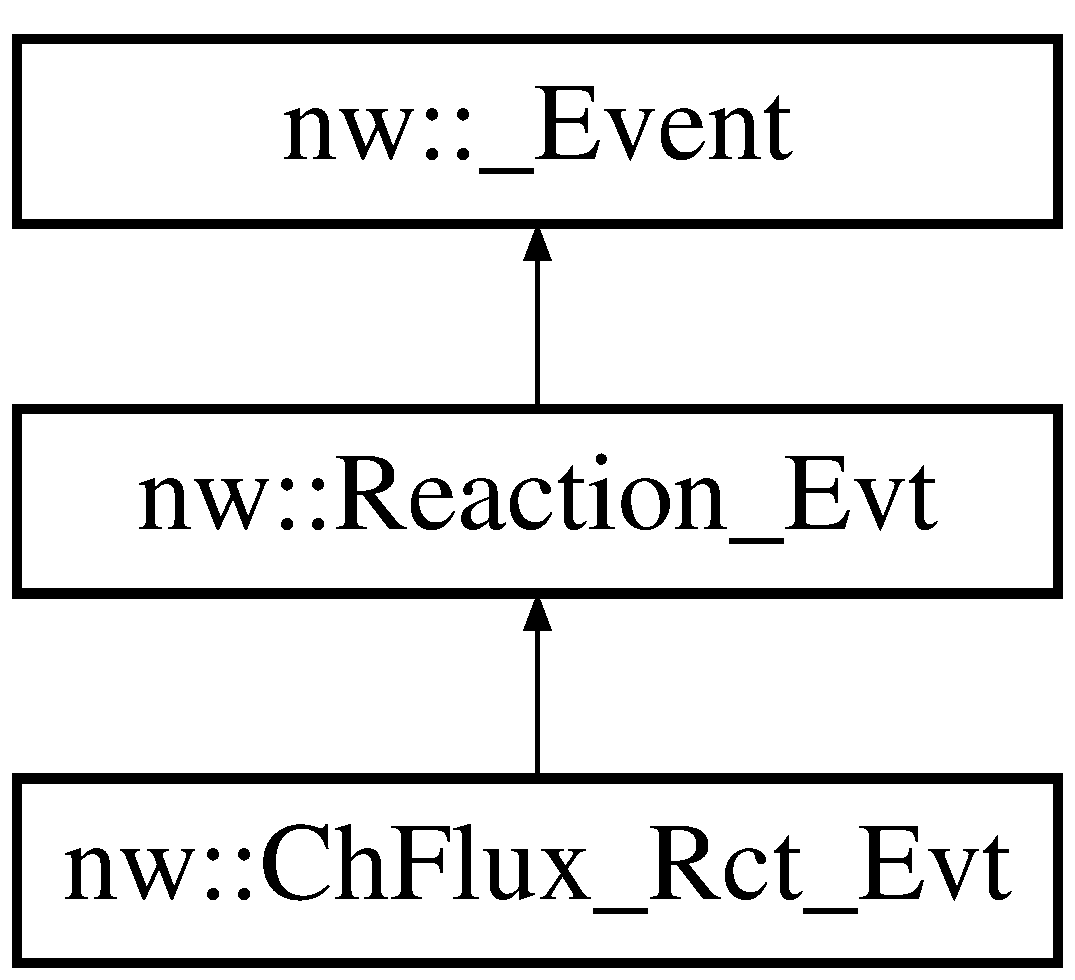
\includegraphics[height=3.000000cm]{de/d56/classnw_1_1_ch_flux___rct___evt}
\end{center}
\end{figure}
\subsection*{Public Member Functions}
\begin{DoxyCompactItemize}
\item 
\hyperlink{classnw_1_1_ch_flux___rct___evt_ab54a4c1b86a428cf540967fc0d575b56}{Ch\+Flux\+\_\+\+Rct\+\_\+\+Evt} (long \hyperlink{classnw_1_1___event_a8f7ce287f596266dd763ec7db2f74090}{id}, string \hyperlink{classnw_1_1___event_ab4f50a54039cd4957bdca55049178562}{name}, double \hyperlink{classnw_1_1___event_afca0ae816e9834add07db8e9a6618faa}{k}, vector$<$ long $>$ \hyperlink{classnw_1_1___event_a560c8b6f9954a43f5d5f80204473b64d}{sc\+\_\+vec}, long \hyperlink{classnw_1_1_ch_flux___rct___evt_a29702aefc95f39082b9d8a9278e3b0f8}{ch\+\_\+spc\+\_\+id}, \hyperlink{namespacenw_ad7146b8b5a9de9be416847f41135722c}{Voxel\+Vector} vvc, \hyperlink{classnw_1_1_uni___rnd}{Uni\+\_\+\+Rnd} $\ast$\hyperlink{classnw_1_1___event_af92482aeea55562560573ecccd5ab108}{rg})
\item 
virtual \hyperlink{classnw_1_1_ch_flux___rct___evt_ada973af5af7cb1ea6c341fd64dd0f850}{$\sim$\+Ch\+Flux\+\_\+\+Rct\+\_\+\+Evt} ()
\item 
void \hyperlink{classnw_1_1_ch_flux___rct___evt_a59d8b2ededb919b5b2cf4358de9a6137}{init} ()
\begin{DoxyCompactList}\small\item\em Implementation of the \hyperlink{classnw_1_1___event_ae2c608ee2508058d6f318ca2ca8f4317}{\+\_\+\+Event\+::init()} method. \end{DoxyCompactList}\item 
double \hyperlink{classnw_1_1_ch_flux___rct___evt_a4034ee90e8ec27a92665a5591fad165d}{update} (double)
\begin{DoxyCompactList}\small\item\em Implementation of the \hyperlink{classnw_1_1___event_a882115f8652c881bc8ed43f1050ccba3}{\+\_\+\+Event\+::update} method. \end{DoxyCompactList}\end{DoxyCompactItemize}
\subsection*{Private Member Functions}
\begin{DoxyCompactItemize}
\item 
double \hyperlink{classnw_1_1_ch_flux___rct___evt_a929abfad936dfc3501b8b5b523112ab9}{calc\+\_\+tau} (long vid)
\end{DoxyCompactItemize}
\subsection*{Private Attributes}
\begin{DoxyCompactItemize}
\item 
long \hyperlink{classnw_1_1_ch_flux___rct___evt_a29702aefc95f39082b9d8a9278e3b0f8}{ch\+\_\+spc\+\_\+id}
\end{DoxyCompactItemize}
\subsection*{Additional Inherited Members}


\subsection{Detailed Description}
Channel flux reaction event. 

This event is derived from the reaction event and introduces the flux of a molecular species through a channel. It differs from an ordinary reaction event due to the fact that the educt (the channel) is not modified by the event itself. Thus the educt vector has to be generated manually in the \hyperlink{classnw_1_1_ch_flux___rct___evt_a59d8b2ededb919b5b2cf4358de9a6137}{init()} function. 

\subsection{Constructor \& Destructor Documentation}
\hypertarget{classnw_1_1_ch_flux___rct___evt_ab54a4c1b86a428cf540967fc0d575b56}{\index{nw\+::\+Ch\+Flux\+\_\+\+Rct\+\_\+\+Evt@{nw\+::\+Ch\+Flux\+\_\+\+Rct\+\_\+\+Evt}!Ch\+Flux\+\_\+\+Rct\+\_\+\+Evt@{Ch\+Flux\+\_\+\+Rct\+\_\+\+Evt}}
\index{Ch\+Flux\+\_\+\+Rct\+\_\+\+Evt@{Ch\+Flux\+\_\+\+Rct\+\_\+\+Evt}!nw\+::\+Ch\+Flux\+\_\+\+Rct\+\_\+\+Evt@{nw\+::\+Ch\+Flux\+\_\+\+Rct\+\_\+\+Evt}}
\subsubsection[{Ch\+Flux\+\_\+\+Rct\+\_\+\+Evt}]{\setlength{\rightskip}{0pt plus 5cm}nw\+::\+Ch\+Flux\+\_\+\+Rct\+\_\+\+Evt\+::\+Ch\+Flux\+\_\+\+Rct\+\_\+\+Evt (
\begin{DoxyParamCaption}
\item[{long}]{id, }
\item[{string}]{name, }
\item[{double}]{k, }
\item[{vector$<$ long $>$}]{sc\+\_\+vec, }
\item[{long}]{ch\+\_\+spc\+\_\+id, }
\item[{{\bf Voxel\+Vector}}]{vvc, }
\item[{{\bf Uni\+\_\+\+Rnd} $\ast$}]{rg}
\end{DoxyParamCaption}
)\hspace{0.3cm}{\ttfamily [inline]}}}\label{classnw_1_1_ch_flux___rct___evt_ab54a4c1b86a428cf540967fc0d575b56}

\begin{DoxyCode}
15     :\hyperlink{classnw_1_1_reaction___evt_a582f3c60366d15e89fdd613abe4bd86d}{Reaction\_Evt}(\textcolor{keywordtype}{id},\hyperlink{classnw_1_1___event_ab4f50a54039cd4957bdca55049178562}{name},\hyperlink{classnw_1_1___event_afca0ae816e9834add07db8e9a6618faa}{k},\hyperlink{classnw_1_1___event_a560c8b6f9954a43f5d5f80204473b64d}{sc\_vec},vvc,\hyperlink{classnw_1_1___event_af92482aeea55562560573ecccd5ab108}{rg})\{
16         this->\hyperlink{classnw_1_1_ch_flux___rct___evt_a29702aefc95f39082b9d8a9278e3b0f8}{ch\_spc\_id} = \hyperlink{classnw_1_1_ch_flux___rct___evt_a29702aefc95f39082b9d8a9278e3b0f8}{ch\_spc\_id};
17     \}
\end{DoxyCode}
\hypertarget{classnw_1_1_ch_flux___rct___evt_ada973af5af7cb1ea6c341fd64dd0f850}{\index{nw\+::\+Ch\+Flux\+\_\+\+Rct\+\_\+\+Evt@{nw\+::\+Ch\+Flux\+\_\+\+Rct\+\_\+\+Evt}!````~Ch\+Flux\+\_\+\+Rct\+\_\+\+Evt@{$\sim$\+Ch\+Flux\+\_\+\+Rct\+\_\+\+Evt}}
\index{````~Ch\+Flux\+\_\+\+Rct\+\_\+\+Evt@{$\sim$\+Ch\+Flux\+\_\+\+Rct\+\_\+\+Evt}!nw\+::\+Ch\+Flux\+\_\+\+Rct\+\_\+\+Evt@{nw\+::\+Ch\+Flux\+\_\+\+Rct\+\_\+\+Evt}}
\subsubsection[{$\sim$\+Ch\+Flux\+\_\+\+Rct\+\_\+\+Evt}]{\setlength{\rightskip}{0pt plus 5cm}virtual nw\+::\+Ch\+Flux\+\_\+\+Rct\+\_\+\+Evt\+::$\sim$\+Ch\+Flux\+\_\+\+Rct\+\_\+\+Evt (
\begin{DoxyParamCaption}
{}
\end{DoxyParamCaption}
)\hspace{0.3cm}{\ttfamily [inline]}, {\ttfamily [virtual]}}}\label{classnw_1_1_ch_flux___rct___evt_ada973af5af7cb1ea6c341fd64dd0f850}

\begin{DoxyCode}
18 \{\};
\end{DoxyCode}


\subsection{Member Function Documentation}
\hypertarget{classnw_1_1_ch_flux___rct___evt_a929abfad936dfc3501b8b5b523112ab9}{\index{nw\+::\+Ch\+Flux\+\_\+\+Rct\+\_\+\+Evt@{nw\+::\+Ch\+Flux\+\_\+\+Rct\+\_\+\+Evt}!calc\+\_\+tau@{calc\+\_\+tau}}
\index{calc\+\_\+tau@{calc\+\_\+tau}!nw\+::\+Ch\+Flux\+\_\+\+Rct\+\_\+\+Evt@{nw\+::\+Ch\+Flux\+\_\+\+Rct\+\_\+\+Evt}}
\subsubsection[{calc\+\_\+tau}]{\setlength{\rightskip}{0pt plus 5cm}double nw\+::\+Ch\+Flux\+\_\+\+Rct\+\_\+\+Evt\+::calc\+\_\+tau (
\begin{DoxyParamCaption}
\item[{long}]{vid}
\end{DoxyParamCaption}
)\hspace{0.3cm}{\ttfamily [private]}}}\label{classnw_1_1_ch_flux___rct___evt_a929abfad936dfc3501b8b5b523112ab9}

\begin{DoxyCode}
43                                        \{
44     \hyperlink{classnw_1_1___event_a6351b58d94923ed58e0b2cf6c9445d2e}{tv\_vec}[vid].t = -log(\hyperlink{classnw_1_1___event_af92482aeea55562560573ecccd5ab108}{rg}->\hyperlink{classnw_1_1_uni___rnd_ad7883ef0ce4c591612bcb41678104773}{get\_Uni\_Rnd}()) / (\hyperlink{classnw_1_1___event_a6351b58d94923ed58e0b2cf6c9445d2e}{tv\_vec}.at(vid).v->get\_state\_vec()->
45                     at(\hyperlink{classnw_1_1_reaction___evt_ae20c8b7d42ef1607200e1e2541db9a70}{educt\_vec}.at(0))->get\_n\_molecules() * \hyperlink{classnw_1_1___event_a29c77fb164e745cdb5c5fda4f191cd37}{c});
46     \textcolor{keywordflow}{return} \hyperlink{classnw_1_1___event_a6351b58d94923ed58e0b2cf6c9445d2e}{tv\_vec}[vid].t;
47 \}
\end{DoxyCode}
\hypertarget{classnw_1_1_ch_flux___rct___evt_a59d8b2ededb919b5b2cf4358de9a6137}{\index{nw\+::\+Ch\+Flux\+\_\+\+Rct\+\_\+\+Evt@{nw\+::\+Ch\+Flux\+\_\+\+Rct\+\_\+\+Evt}!init@{init}}
\index{init@{init}!nw\+::\+Ch\+Flux\+\_\+\+Rct\+\_\+\+Evt@{nw\+::\+Ch\+Flux\+\_\+\+Rct\+\_\+\+Evt}}
\subsubsection[{init}]{\setlength{\rightskip}{0pt plus 5cm}void nw\+::\+Ch\+Flux\+\_\+\+Rct\+\_\+\+Evt\+::init (
\begin{DoxyParamCaption}
{}
\end{DoxyParamCaption}
)\hspace{0.3cm}{\ttfamily [virtual]}}}\label{classnw_1_1_ch_flux___rct___evt_a59d8b2ededb919b5b2cf4358de9a6137}


Implementation of the \hyperlink{classnw_1_1___event_ae2c608ee2508058d6f318ca2ca8f4317}{\+\_\+\+Event\+::init()} method. 

The educt of this first order reaction is not modified by the event itself. The educt vector has therefore to be generated manually. 

Implements \hyperlink{classnw_1_1___event_ae2c608ee2508058d6f318ca2ca8f4317}{nw\+::\+\_\+\+Event}.


\begin{DoxyCode}
6                          \{
7     \hyperlink{classnw_1_1_reaction___evt_ae20c8b7d42ef1607200e1e2541db9a70}{educt\_vec}.push\_back(\hyperlink{classnw_1_1_ch_flux___rct___evt_a29702aefc95f39082b9d8a9278e3b0f8}{ch\_spc\_id});
8     \hyperlink{classnw_1_1___event_a29c77fb164e745cdb5c5fda4f191cd37}{c}=\hyperlink{classnw_1_1___event_afca0ae816e9834add07db8e9a6618faa}{k};
9     \hyperlink{classnw_1_1_ch_flux___rct___evt_a4034ee90e8ec27a92665a5591fad165d}{update}(0);
10 \}
\end{DoxyCode}
\hypertarget{classnw_1_1_ch_flux___rct___evt_a4034ee90e8ec27a92665a5591fad165d}{\index{nw\+::\+Ch\+Flux\+\_\+\+Rct\+\_\+\+Evt@{nw\+::\+Ch\+Flux\+\_\+\+Rct\+\_\+\+Evt}!update@{update}}
\index{update@{update}!nw\+::\+Ch\+Flux\+\_\+\+Rct\+\_\+\+Evt@{nw\+::\+Ch\+Flux\+\_\+\+Rct\+\_\+\+Evt}}
\subsubsection[{update}]{\setlength{\rightskip}{0pt plus 5cm}double nw\+::\+Ch\+Flux\+\_\+\+Rct\+\_\+\+Evt\+::update (
\begin{DoxyParamCaption}
\item[{double}]{last\+\_\+tau}
\end{DoxyParamCaption}
)\hspace{0.3cm}{\ttfamily [virtual]}}}\label{classnw_1_1_ch_flux___rct___evt_a4034ee90e8ec27a92665a5591fad165d}


Implementation of the \hyperlink{classnw_1_1___event_a882115f8652c881bc8ed43f1050ccba3}{\+\_\+\+Event\+::update} method. 

\begin{DoxyReturn}{Returns}
New tau value for this \hyperlink{classnw_1_1___event}{\+\_\+\+Event} 
\end{DoxyReturn}

\begin{DoxyParams}{Parameters}
{\em last\+\_\+tau} & Tau value of previous firing \hyperlink{classnw_1_1___event}{\+\_\+\+Event}\\
\hline
\end{DoxyParams}
The channel flux reaction event differs from its mother class in its update function. ~\newline
~\newline
Note\+: This event cannot be part of the dependency graph, because there is no event that causes a new number of open channels. A new tau value is calculated every simulation step. This is a sub-\/optimal implementation. One option is to manually add this event to the dependency graph of the sub\+Unit\+Switch reaction. 

Implements \hyperlink{classnw_1_1___event_a882115f8652c881bc8ed43f1050ccba3}{nw\+::\+\_\+\+Event}.


\begin{DoxyCode}
12                                             \{
13 
14     \textcolor{keywordtype}{double} minTau = INFINITY;
15     \textcolor{keywordtype}{double} actTau;
16 
17 \textcolor{comment}{//  run through the tv vector}
18     \textcolor{keywordflow}{for} (\textcolor{keywordtype}{long} i = 0; i < (long) \hyperlink{classnw_1_1___event_a6351b58d94923ed58e0b2cf6c9445d2e}{tv\_vec}.size(); i++) \{
19 \textcolor{comment}{//      check for voxel that have been affected by last executed event}
20         \textcolor{keywordflow}{if} (\hyperlink{classnw_1_1___event_a6351b58d94923ed58e0b2cf6c9445d2e}{tv\_vec}.at(i).v->get\_dirty\_flag()) \{
21             actTau = \hyperlink{classnw_1_1_ch_flux___rct___evt_a929abfad936dfc3501b8b5b523112ab9}{calc\_tau}(i);
22 \textcolor{comment}{//          find smallest tau value (->next voxel) for this event}
23             \textcolor{keywordflow}{if} (actTau < minTau) \{
24                 minTau = actTau;
25                 \hyperlink{classnw_1_1___event_a7864559e204c087306e3becb5b81fb26}{nextVoxel} = i;
26             \}
27 \textcolor{comment}{//      this voxel has not been affected by last event}
28         \} \textcolor{keywordflow}{else} \{
29 \textcolor{comment}{//          adjust tau value to global times scale}
30             \hyperlink{classnw_1_1___event_a6351b58d94923ed58e0b2cf6c9445d2e}{tv\_vec}.at(i).t -= last\_tau;
31 \textcolor{comment}{//          find smallest tau value (->next voxel) for this event}
32             \textcolor{keywordflow}{if} (\hyperlink{classnw_1_1___event_a6351b58d94923ed58e0b2cf6c9445d2e}{tv\_vec}[i].t < minTau) \{
33                 minTau = \hyperlink{classnw_1_1___event_a6351b58d94923ed58e0b2cf6c9445d2e}{tv\_vec}[i].t;
34                 \hyperlink{classnw_1_1___event_a7864559e204c087306e3becb5b81fb26}{nextVoxel} = i;
35             \}
36         \}
37     \}
38     this->\hyperlink{classnw_1_1___event_aaa705b35c06c0cb2e0a4f3daa9ee8037}{dirty\_flag} = \textcolor{keyword}{false};
39 
40     \textcolor{keywordflow}{return} minTau;
41 \}
\end{DoxyCode}


\subsection{Member Data Documentation}
\hypertarget{classnw_1_1_ch_flux___rct___evt_a29702aefc95f39082b9d8a9278e3b0f8}{\index{nw\+::\+Ch\+Flux\+\_\+\+Rct\+\_\+\+Evt@{nw\+::\+Ch\+Flux\+\_\+\+Rct\+\_\+\+Evt}!ch\+\_\+spc\+\_\+id@{ch\+\_\+spc\+\_\+id}}
\index{ch\+\_\+spc\+\_\+id@{ch\+\_\+spc\+\_\+id}!nw\+::\+Ch\+Flux\+\_\+\+Rct\+\_\+\+Evt@{nw\+::\+Ch\+Flux\+\_\+\+Rct\+\_\+\+Evt}}
\subsubsection[{ch\+\_\+spc\+\_\+id}]{\setlength{\rightskip}{0pt plus 5cm}long nw\+::\+Ch\+Flux\+\_\+\+Rct\+\_\+\+Evt\+::ch\+\_\+spc\+\_\+id\hspace{0.3cm}{\ttfamily [private]}}}\label{classnw_1_1_ch_flux___rct___evt_a29702aefc95f39082b9d8a9278e3b0f8}


The documentation for this class was generated from the following files\+:\begin{DoxyCompactItemize}
\item 
Events/\hyperlink{_ch_flux___rct___evt_8h}{Ch\+Flux\+\_\+\+Rct\+\_\+\+Evt.\+h}\item 
Events/\hyperlink{_ch_flux___rct___evt_8cpp}{Ch\+Flux\+\_\+\+Rct\+\_\+\+Evt.\+cpp}\end{DoxyCompactItemize}

\hypertarget{classnw_1_1_diffusion___evt}{\section{nw\+:\+:Diffusion\+\_\+\+Evt Class Reference}
\label{classnw_1_1_diffusion___evt}\index{nw\+::\+Diffusion\+\_\+\+Evt@{nw\+::\+Diffusion\+\_\+\+Evt}}
}


Realization of diffusion between two voxels.  




{\ttfamily \#include $<$Diffusion\+\_\+\+Evt.\+h$>$}

Inheritance diagram for nw\+:\+:Diffusion\+\_\+\+Evt\+:\begin{figure}[H]
\begin{center}
\leavevmode
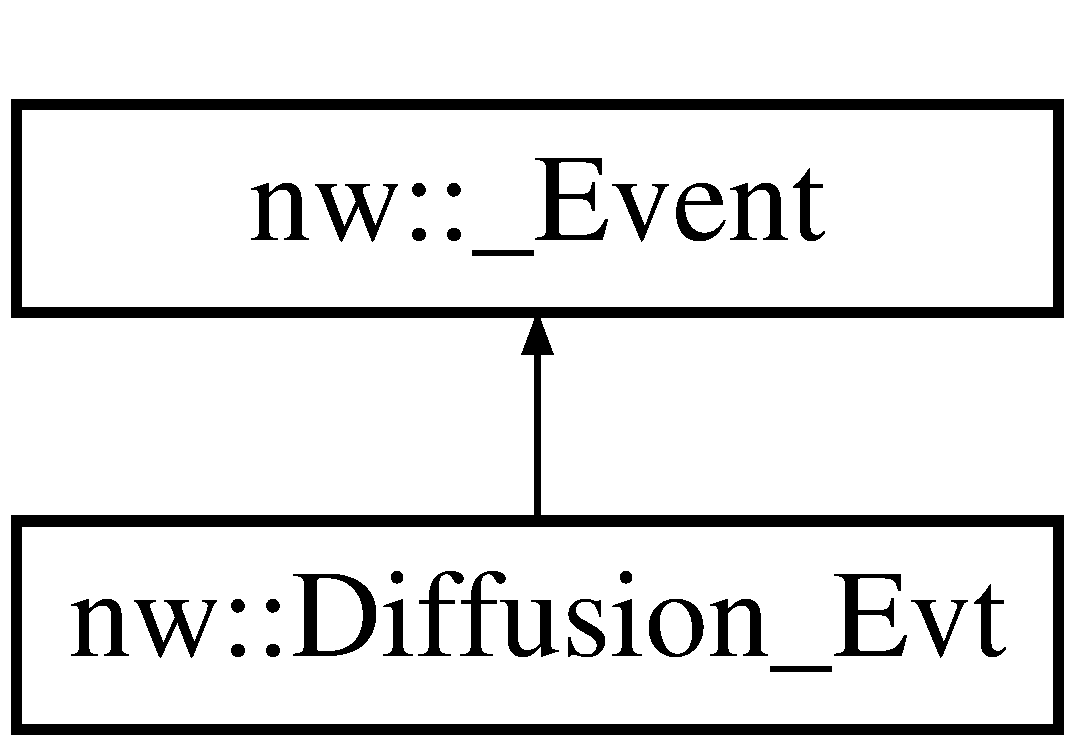
\includegraphics[height=2.000000cm]{db/d40/classnw_1_1_diffusion___evt}
\end{center}
\end{figure}
\subsection*{Public Member Functions}
\begin{DoxyCompactItemize}
\item 
\hyperlink{classnw_1_1_diffusion___evt_aa7a2892e0b8c19e58df2a37ab71213cc}{Diffusion\+\_\+\+Evt} (long \hyperlink{classnw_1_1___event_a8f7ce287f596266dd763ec7db2f74090}{id}, string \hyperlink{classnw_1_1___event_ab4f50a54039cd4957bdca55049178562}{name}, double \hyperlink{classnw_1_1___event_afca0ae816e9834add07db8e9a6618faa}{k}, \hyperlink{namespacenw_ad7146b8b5a9de9be416847f41135722c}{Voxel\+Vector} vvc, long diff\+\_\+spc\+\_\+id, \hyperlink{classnw_1_1_uni___rnd}{Uni\+\_\+\+Rnd} $\ast$\hyperlink{classnw_1_1___event_af92482aeea55562560573ecccd5ab108}{rg})
\begin{DoxyCompactList}\small\item\em Constructor of Diffusion Event. \end{DoxyCompactList}\item 
virtual \hyperlink{classnw_1_1_diffusion___evt_a13608fc5a0cbe6e77caeca4cd77def61}{$\sim$\+Diffusion\+\_\+\+Evt} ()
\item 
double \hyperlink{classnw_1_1_diffusion___evt_a35841daf14d9ba472c0ed1f414187097}{update} (double)
\begin{DoxyCompactList}\small\item\em Diffusion implementation of \hyperlink{classnw_1_1___event_a882115f8652c881bc8ed43f1050ccba3}{\+\_\+\+Event\+::update()} method. \end{DoxyCompactList}\item 
void \hyperlink{classnw_1_1_diffusion___evt_a5cd6413241bd01ecb6a58fc0359ab57b}{execute} ()
\begin{DoxyCompactList}\small\item\em Diffusion implementation of \hyperlink{classnw_1_1___event_aa022418fb765582a053ac75cbc3436d6}{\+\_\+\+Event\+::execute()} method. \end{DoxyCompactList}\item 
void \hyperlink{classnw_1_1_diffusion___evt_adaaca9b5b7e6902189dfc79d8d5a4f99}{init} ()
\begin{DoxyCompactList}\small\item\em Diffusion implementation of \hyperlink{classnw_1_1___event_ae2c608ee2508058d6f318ca2ca8f4317}{\+\_\+\+Event\+::init()} method initializes a diffusion. State change vector is generated and the event propensity is calculated. \end{DoxyCompactList}\item 
double \hyperlink{classnw_1_1_diffusion___evt_a468711cd0c37b2129898cb8e79c2f085}{get\+\_\+a} ()
\begin{DoxyCompactList}\small\item\em Diffusion implementation of \hyperlink{classnw_1_1___event_a75945699f539cefab36eb6693a389918}{\+\_\+\+Event\+::get\+\_\+a()} method. \end{DoxyCompactList}\end{DoxyCompactItemize}
\subsection*{Protected Member Functions}
\begin{DoxyCompactItemize}
\item 
double \hyperlink{classnw_1_1_diffusion___evt_a45b4ac64dd8f202de5b1e590b7a88621}{calc\+\_\+tau} (long)
\begin{DoxyCompactList}\small\item\em function to calculate next tau value of a voxel. \end{DoxyCompactList}\item 
void \hyperlink{classnw_1_1_diffusion___evt_a207aa73a53839282e1a399b5d4d7c3d1}{build\+\_\+sc\+\_\+vec} ()
\begin{DoxyCompactList}\small\item\em builds the state change vector and the inverse state change vector of the diffusion event. \end{DoxyCompactList}\end{DoxyCompactItemize}
\subsection*{Protected Attributes}
\begin{DoxyCompactItemize}
\item 
vector$<$ long $>$ \hyperlink{classnw_1_1_diffusion___evt_ab975d8f0ae97844b4d43222e94871707}{inv\+\_\+sc\+\_\+vec}
\begin{DoxyCompactList}\small\item\em inverse sc\+\_\+vec to update origin diffusion voxel ($\ast$ -\/1) \end{DoxyCompactList}\item 
long \hyperlink{classnw_1_1_diffusion___evt_a7193335899a1d41a902dff91fc0029dd}{diff\+\_\+spec\+\_\+id}
\begin{DoxyCompactList}\small\item\em id of the species which diffusion is represented by this Event \end{DoxyCompactList}\end{DoxyCompactItemize}


\subsection{Detailed Description}
Realization of diffusion between two voxels. 

The Diffusion\+\_\+\+Event alters the stae vector of two adjacent Voxel. The \hyperlink{classnw_1_1_diffusion___evt_a5cd6413241bd01ecb6a58fc0359ab57b}{execute()} function thus needs a second random number to determine the diffusion partner from the voxel diff list. 

\subsection{Constructor \& Destructor Documentation}
\hypertarget{classnw_1_1_diffusion___evt_aa7a2892e0b8c19e58df2a37ab71213cc}{\index{nw\+::\+Diffusion\+\_\+\+Evt@{nw\+::\+Diffusion\+\_\+\+Evt}!Diffusion\+\_\+\+Evt@{Diffusion\+\_\+\+Evt}}
\index{Diffusion\+\_\+\+Evt@{Diffusion\+\_\+\+Evt}!nw\+::\+Diffusion\+\_\+\+Evt@{nw\+::\+Diffusion\+\_\+\+Evt}}
\subsubsection[{Diffusion\+\_\+\+Evt}]{\setlength{\rightskip}{0pt plus 5cm}nw\+::\+Diffusion\+\_\+\+Evt\+::\+Diffusion\+\_\+\+Evt (
\begin{DoxyParamCaption}
\item[{long}]{id, }
\item[{string}]{name, }
\item[{double}]{k, }
\item[{{\bf Voxel\+Vector}}]{vvc, }
\item[{long}]{diff\+\_\+spc\+\_\+id, }
\item[{{\bf Uni\+\_\+\+Rnd} $\ast$}]{rg}
\end{DoxyParamCaption}
)\hspace{0.3cm}{\ttfamily [inline]}}}\label{classnw_1_1_diffusion___evt_aa7a2892e0b8c19e58df2a37ab71213cc}


Constructor of Diffusion Event. 


\begin{DoxyParams}{Parameters}
{\em id} & \hyperlink{classnw_1_1___event}{\+\_\+\+Event} I\+D \\
\hline
{\em name} & \hyperlink{classnw_1_1___event}{\+\_\+\+Event} name \\
\hline
{\em k} & \hyperlink{classnw_1_1___event}{\+\_\+\+Event} rate constant \\
\hline
{\em vvc} & vector of all voxel where this event can occur \\
\hline
{\em diff\+\_\+spc\+\_\+id} & indicates the id of the diffusing molecule species \\
\hline
{\em rg} & Pointer to the Random\+\_\+\+Generator \\
\hline
\end{DoxyParams}

\begin{DoxyCode}
26                                                                                                 :
27         \hyperlink{classnw_1_1___event_a5efb757db20b083de6da605ea4b2bbae}{\_Event}(\textcolor{keywordtype}{id},\hyperlink{classnw_1_1___event_ab4f50a54039cd4957bdca55049178562}{name},\hyperlink{classnw_1_1___event_afca0ae816e9834add07db8e9a6618faa}{k},vvc,\hyperlink{classnw_1_1___event_af92482aeea55562560573ecccd5ab108}{rg})\{
28         this->\hyperlink{classnw_1_1_diffusion___evt_a7193335899a1d41a902dff91fc0029dd}{diff\_spec\_id} = diff\_spc\_id;
29         \hyperlink{classnw_1_1_diffusion___evt_a207aa73a53839282e1a399b5d4d7c3d1}{build\_sc\_vec}();
30     \}
\end{DoxyCode}
\hypertarget{classnw_1_1_diffusion___evt_a13608fc5a0cbe6e77caeca4cd77def61}{\index{nw\+::\+Diffusion\+\_\+\+Evt@{nw\+::\+Diffusion\+\_\+\+Evt}!````~Diffusion\+\_\+\+Evt@{$\sim$\+Diffusion\+\_\+\+Evt}}
\index{````~Diffusion\+\_\+\+Evt@{$\sim$\+Diffusion\+\_\+\+Evt}!nw\+::\+Diffusion\+\_\+\+Evt@{nw\+::\+Diffusion\+\_\+\+Evt}}
\subsubsection[{$\sim$\+Diffusion\+\_\+\+Evt}]{\setlength{\rightskip}{0pt plus 5cm}virtual nw\+::\+Diffusion\+\_\+\+Evt\+::$\sim$\+Diffusion\+\_\+\+Evt (
\begin{DoxyParamCaption}
{}
\end{DoxyParamCaption}
)\hspace{0.3cm}{\ttfamily [inline]}, {\ttfamily [virtual]}}}\label{classnw_1_1_diffusion___evt_a13608fc5a0cbe6e77caeca4cd77def61}
Destructor 
\begin{DoxyCode}
32 \{\};
\end{DoxyCode}


\subsection{Member Function Documentation}
\hypertarget{classnw_1_1_diffusion___evt_a207aa73a53839282e1a399b5d4d7c3d1}{\index{nw\+::\+Diffusion\+\_\+\+Evt@{nw\+::\+Diffusion\+\_\+\+Evt}!build\+\_\+sc\+\_\+vec@{build\+\_\+sc\+\_\+vec}}
\index{build\+\_\+sc\+\_\+vec@{build\+\_\+sc\+\_\+vec}!nw\+::\+Diffusion\+\_\+\+Evt@{nw\+::\+Diffusion\+\_\+\+Evt}}
\subsubsection[{build\+\_\+sc\+\_\+vec}]{\setlength{\rightskip}{0pt plus 5cm}void nw\+::\+Diffusion\+\_\+\+Evt\+::build\+\_\+sc\+\_\+vec (
\begin{DoxyParamCaption}
{}
\end{DoxyParamCaption}
)\hspace{0.3cm}{\ttfamily [protected]}}}\label{classnw_1_1_diffusion___evt_a207aa73a53839282e1a399b5d4d7c3d1}


builds the state change vector and the inverse state change vector of the diffusion event. 

Helper function to build an inverse sc\+\_\+vector. Number of molecules in the origin Voxel has to be decreased, while number of molecules in the target voxel has to be increased. Thus \hyperlink{classnw_1_1_diffusion___evt}{Diffusion\+\_\+\+Evt} requires two state change vectors.\+builds a state change vector using diff\+\_\+spec\+\_\+id 
\begin{DoxyCode}
85                                 \{
86 \textcolor{comment}{//  build sc\_vec}
87     \hyperlink{classnw_1_1___event_a560c8b6f9954a43f5d5f80204473b64d}{sc\_vec}.assign(\hyperlink{classnw_1_1___event_a6351b58d94923ed58e0b2cf6c9445d2e}{tv\_vec}[0].v->get\_state\_vec()->size(),0);
88     \hyperlink{classnw_1_1_diffusion___evt_ab975d8f0ae97844b4d43222e94871707}{inv\_sc\_vec}.assign(\hyperlink{classnw_1_1___event_a6351b58d94923ed58e0b2cf6c9445d2e}{tv\_vec}[0].v->get\_state\_vec()->size(),0);
89     \hyperlink{classnw_1_1___event_a560c8b6f9954a43f5d5f80204473b64d}{sc\_vec}[\hyperlink{classnw_1_1_diffusion___evt_a7193335899a1d41a902dff91fc0029dd}{diff\_spec\_id}] = -1;
90     \hyperlink{classnw_1_1_diffusion___evt_ab975d8f0ae97844b4d43222e94871707}{inv\_sc\_vec}[\hyperlink{classnw_1_1_diffusion___evt_a7193335899a1d41a902dff91fc0029dd}{diff\_spec\_id}] = 1;
91 
92 \}
\end{DoxyCode}
\hypertarget{classnw_1_1_diffusion___evt_a45b4ac64dd8f202de5b1e590b7a88621}{\index{nw\+::\+Diffusion\+\_\+\+Evt@{nw\+::\+Diffusion\+\_\+\+Evt}!calc\+\_\+tau@{calc\+\_\+tau}}
\index{calc\+\_\+tau@{calc\+\_\+tau}!nw\+::\+Diffusion\+\_\+\+Evt@{nw\+::\+Diffusion\+\_\+\+Evt}}
\subsubsection[{calc\+\_\+tau}]{\setlength{\rightskip}{0pt plus 5cm}double nw\+::\+Diffusion\+\_\+\+Evt\+::calc\+\_\+tau (
\begin{DoxyParamCaption}
\item[{long}]{vid}
\end{DoxyParamCaption}
)\hspace{0.3cm}{\ttfamily [protected]}}}\label{classnw_1_1_diffusion___evt_a45b4ac64dd8f202de5b1e590b7a88621}


function to calculate next tau value of a voxel. 


\begin{DoxyParams}{Parameters}
{\em vid} & the Voxel id of the voxel which has to be updated \\
\hline
\end{DoxyParams}
\begin{DoxyReturn}{Returns}
new tau value 
\end{DoxyReturn}

\begin{DoxyCode}
94                                       \{
95 \textcolor{comment}{//  adapt the c value to the number of diffusion sites!}
96     \textcolor{keywordtype}{double} c\_adapted =  \hyperlink{classnw_1_1___event_a29c77fb164e745cdb5c5fda4f191cd37}{c} * \hyperlink{classnw_1_1___event_a6351b58d94923ed58e0b2cf6c9445d2e}{tv\_vec}.at(vid).v->get\_diff\_vec()->size();
97 \textcolor{comment}{//  calculate tau}
98     \hyperlink{classnw_1_1___event_a6351b58d94923ed58e0b2cf6c9445d2e}{tv\_vec}[vid].t = -log(\hyperlink{classnw_1_1___event_af92482aeea55562560573ecccd5ab108}{rg}->\hyperlink{classnw_1_1_uni___rnd_ad7883ef0ce4c591612bcb41678104773}{get\_Uni\_Rnd}()) / (\hyperlink{classnw_1_1___event_a6351b58d94923ed58e0b2cf6c9445d2e}{tv\_vec}[vid].v->get\_state\_vec()->at(
      \hyperlink{classnw_1_1_diffusion___evt_a7193335899a1d41a902dff91fc0029dd}{diff\_spec\_id})->get\_n\_molecules() * c\_adapted);
99 
100     \textcolor{keywordflow}{return} \hyperlink{classnw_1_1___event_a6351b58d94923ed58e0b2cf6c9445d2e}{tv\_vec}[vid].t;
101 \}
\end{DoxyCode}
\hypertarget{classnw_1_1_diffusion___evt_a5cd6413241bd01ecb6a58fc0359ab57b}{\index{nw\+::\+Diffusion\+\_\+\+Evt@{nw\+::\+Diffusion\+\_\+\+Evt}!execute@{execute}}
\index{execute@{execute}!nw\+::\+Diffusion\+\_\+\+Evt@{nw\+::\+Diffusion\+\_\+\+Evt}}
\subsubsection[{execute}]{\setlength{\rightskip}{0pt plus 5cm}void nw\+::\+Diffusion\+\_\+\+Evt\+::execute (
\begin{DoxyParamCaption}
{}
\end{DoxyParamCaption}
)\hspace{0.3cm}{\ttfamily [virtual]}}}\label{classnw_1_1_diffusion___evt_a5cd6413241bd01ecb6a58fc0359ab57b}


Diffusion implementation of \hyperlink{classnw_1_1___event_aa022418fb765582a053ac75cbc3436d6}{\+\_\+\+Event\+::execute()} method. 

Two voxels have to be updated. Decrease the number of molecules by one inside the origin voxel and increase the number of molecules by one in the target voxel. The target voxel is determined randomly from the diffusion vector that defines the vicinity relation of different voxel. 

Implements \hyperlink{classnw_1_1___event_aa022418fb765582a053ac75cbc3436d6}{nw\+::\+\_\+\+Event}.


\begin{DoxyCode}
21                            \{
22 \textcolor{comment}{//  update diffusion origin voxel with the inverse state change vector}
23     \hyperlink{classnw_1_1___event_a6351b58d94923ed58e0b2cf6c9445d2e}{tv\_vec}[\hyperlink{classnw_1_1___event_a7864559e204c087306e3becb5b81fb26}{nextVoxel}].v->update\_state(\hyperlink{classnw_1_1___event_a560c8b6f9954a43f5d5f80204473b64d}{sc\_vec});
24 
25 \textcolor{comment}{//  choose diffusion partner}
26     \textcolor{keywordtype}{double} r = \hyperlink{classnw_1_1___event_af92482aeea55562560573ecccd5ab108}{rg}->\hyperlink{classnw_1_1_uni___rnd_ad7883ef0ce4c591612bcb41678104773}{get\_Uni\_Rnd}();
27     \textcolor{keywordtype}{double} d; \textcolor{comment}{// temp}
28     \textcolor{keywordflow}{for} (\textcolor{keywordtype}{size\_t} i = 0; i < \hyperlink{classnw_1_1___event_a6351b58d94923ed58e0b2cf6c9445d2e}{tv\_vec}[\hyperlink{classnw_1_1___event_a7864559e204c087306e3becb5b81fb26}{nextVoxel}].v->get\_diff\_vec()->size(); ++i)\{
29         d = (double)(i+1)/\hyperlink{classnw_1_1___event_a6351b58d94923ed58e0b2cf6c9445d2e}{tv\_vec}[\hyperlink{classnw_1_1___event_a7864559e204c087306e3becb5b81fb26}{nextVoxel}].v->get\_diff\_vec()->size();
30         \textcolor{keywordflow}{if}(r-d < 0)\{
31             \hyperlink{classnw_1_1___event_a6351b58d94923ed58e0b2cf6c9445d2e}{tv\_vec}[\hyperlink{classnw_1_1___event_a7864559e204c087306e3becb5b81fb26}{nextVoxel}].v->get\_diff\_vec()->at(i)->update\_state(
      \hyperlink{classnw_1_1_diffusion___evt_ab975d8f0ae97844b4d43222e94871707}{inv\_sc\_vec});
32             \textcolor{keywordflow}{break};
33         \}
34     \}
35 
36 \textcolor{comment}{//  set dirty flag to indicate that dependent events have to be updated properly}
37     \textcolor{keywordflow}{for}(\textcolor{keywordtype}{size\_t} i = 0; i < \hyperlink{classnw_1_1___event_a3f87b2dff69d07977f0a5e10936f38f6}{dep\_list}.size(); i++)\{
38         \hyperlink{classnw_1_1___event_a3f87b2dff69d07977f0a5e10936f38f6}{dep\_list}[i]->set\_flag(\textcolor{keyword}{true});
39     \}
40 \}
\end{DoxyCode}
\hypertarget{classnw_1_1_diffusion___evt_a468711cd0c37b2129898cb8e79c2f085}{\index{nw\+::\+Diffusion\+\_\+\+Evt@{nw\+::\+Diffusion\+\_\+\+Evt}!get\+\_\+a@{get\+\_\+a}}
\index{get\+\_\+a@{get\+\_\+a}!nw\+::\+Diffusion\+\_\+\+Evt@{nw\+::\+Diffusion\+\_\+\+Evt}}
\subsubsection[{get\+\_\+a}]{\setlength{\rightskip}{0pt plus 5cm}double nw\+::\+Diffusion\+\_\+\+Evt\+::get\+\_\+a (
\begin{DoxyParamCaption}
{}
\end{DoxyParamCaption}
)\hspace{0.3cm}{\ttfamily [virtual]}}}\label{classnw_1_1_diffusion___evt_a468711cd0c37b2129898cb8e79c2f085}


Diffusion implementation of \hyperlink{classnw_1_1___event_a75945699f539cefab36eb6693a389918}{\+\_\+\+Event\+::get\+\_\+a()} method. 



Implements \hyperlink{classnw_1_1___event_a75945699f539cefab36eb6693a389918}{nw\+::\+\_\+\+Event}.


\begin{DoxyCode}
103                            \{
104     \textcolor{keywordtype}{double} a\_ges = 0;
105     \textcolor{keywordflow}{for}(\textcolor{keywordtype}{long} i = 0; i < (long) \hyperlink{classnw_1_1___event_a6351b58d94923ed58e0b2cf6c9445d2e}{tv\_vec}.size(); i++)\{
106         a\_ges += \hyperlink{classnw_1_1___event_a29c77fb164e745cdb5c5fda4f191cd37}{c}*\hyperlink{classnw_1_1___event_a6351b58d94923ed58e0b2cf6c9445d2e}{tv\_vec}[i].v->get\_state\_vec()->at(\hyperlink{classnw_1_1_diffusion___evt_a7193335899a1d41a902dff91fc0029dd}{diff\_spec\_id})->get\_n\_molecules() * 
      \hyperlink{classnw_1_1___event_a6351b58d94923ed58e0b2cf6c9445d2e}{tv\_vec}[i].v->get\_diff\_vec()->size();
107     \}
108     \textcolor{keywordflow}{return} a\_ges;
109 \}
\end{DoxyCode}
\hypertarget{classnw_1_1_diffusion___evt_adaaca9b5b7e6902189dfc79d8d5a4f99}{\index{nw\+::\+Diffusion\+\_\+\+Evt@{nw\+::\+Diffusion\+\_\+\+Evt}!init@{init}}
\index{init@{init}!nw\+::\+Diffusion\+\_\+\+Evt@{nw\+::\+Diffusion\+\_\+\+Evt}}
\subsubsection[{init}]{\setlength{\rightskip}{0pt plus 5cm}void nw\+::\+Diffusion\+\_\+\+Evt\+::init (
\begin{DoxyParamCaption}
{}
\end{DoxyParamCaption}
)\hspace{0.3cm}{\ttfamily [virtual]}}}\label{classnw_1_1_diffusion___evt_adaaca9b5b7e6902189dfc79d8d5a4f99}


Diffusion implementation of \hyperlink{classnw_1_1___event_ae2c608ee2508058d6f318ca2ca8f4317}{\+\_\+\+Event\+::init()} method initializes a diffusion. State change vector is generated and the event propensity is calculated. 



Implements \hyperlink{classnw_1_1___event_ae2c608ee2508058d6f318ca2ca8f4317}{nw\+::\+\_\+\+Event}.


\begin{DoxyCode}
9                         \{
10 
11 \textcolor{comment}{//  calculate the correct diffusion probability constant according to the voxel volume}
12     this->\hyperlink{classnw_1_1___event_a29c77fb164e745cdb5c5fda4f191cd37}{c} = (\hyperlink{classnw_1_1___event_afca0ae816e9834add07db8e9a6618faa}{k}*1e-3)/pow(\hyperlink{classnw_1_1___event_a6351b58d94923ed58e0b2cf6c9445d2e}{tv\_vec}[0].v->get\_box\_length()*1e6,2);
13 
14 \textcolor{comment}{//  build state change vector}
15     \hyperlink{classnw_1_1_diffusion___evt_a207aa73a53839282e1a399b5d4d7c3d1}{build\_sc\_vec}();
16 
17 \textcolor{comment}{//  update the first time}
18     \hyperlink{classnw_1_1_diffusion___evt_a35841daf14d9ba472c0ed1f414187097}{update}(0);
19 \}
\end{DoxyCode}
\hypertarget{classnw_1_1_diffusion___evt_a35841daf14d9ba472c0ed1f414187097}{\index{nw\+::\+Diffusion\+\_\+\+Evt@{nw\+::\+Diffusion\+\_\+\+Evt}!update@{update}}
\index{update@{update}!nw\+::\+Diffusion\+\_\+\+Evt@{nw\+::\+Diffusion\+\_\+\+Evt}}
\subsubsection[{update}]{\setlength{\rightskip}{0pt plus 5cm}double nw\+::\+Diffusion\+\_\+\+Evt\+::update (
\begin{DoxyParamCaption}
\item[{double}]{last\+\_\+tau}
\end{DoxyParamCaption}
)\hspace{0.3cm}{\ttfamily [virtual]}}}\label{classnw_1_1_diffusion___evt_a35841daf14d9ba472c0ed1f414187097}


Diffusion implementation of \hyperlink{classnw_1_1___event_a882115f8652c881bc8ed43f1050ccba3}{\+\_\+\+Event\+::update()} method. 



Implements \hyperlink{classnw_1_1___event_a882115f8652c881bc8ed43f1050ccba3}{nw\+::\+\_\+\+Event}.


\begin{DoxyCode}
42                                            \{
43 
44     \textcolor{keywordtype}{double} minTau = INFINITY, actTau;
45 
46 \textcolor{comment}{//  check if this event depends on the last executed event}
47     \textcolor{keywordflow}{if} (this->\hyperlink{classnw_1_1___event_aaa705b35c06c0cb2e0a4f3daa9ee8037}{dirty\_flag}) \{
48 \textcolor{comment}{//      run through the tv vector}
49         \textcolor{keywordflow}{for} (\textcolor{keywordtype}{size\_t} i = 0; i < \hyperlink{classnw_1_1___event_a6351b58d94923ed58e0b2cf6c9445d2e}{tv\_vec}.size(); ++i) \{
50 \textcolor{comment}{//          check for voxel that have been affected by last executed event}
51             \textcolor{keywordflow}{if} (\hyperlink{classnw_1_1___event_a6351b58d94923ed58e0b2cf6c9445d2e}{tv\_vec}[i].v->get\_dirty\_flag()) \{
52                 actTau = \hyperlink{classnw_1_1_diffusion___evt_a45b4ac64dd8f202de5b1e590b7a88621}{calc\_tau}(i);
53 \textcolor{comment}{//              find smallest tau value (->next voxel) for this event}
54                 \textcolor{keywordflow}{if} (actTau < minTau) \{
55                     minTau = actTau;
56                     \hyperlink{classnw_1_1___event_a7864559e204c087306e3becb5b81fb26}{nextVoxel} = i;
57                 \}
58 \textcolor{comment}{//          voxel has not been affected by last event}
59             \} \textcolor{keywordflow}{else} \{
60 \textcolor{comment}{//              adjust tau value to global times scale}
61                 \hyperlink{classnw_1_1___event_a6351b58d94923ed58e0b2cf6c9445d2e}{tv\_vec}[i].t -= last\_tau;
62 \textcolor{comment}{//              find smallest tau value (->next voxel) for this event}
63                 \textcolor{keywordflow}{if} (\hyperlink{classnw_1_1___event_a6351b58d94923ed58e0b2cf6c9445d2e}{tv\_vec}[i].t < minTau) \{
64                     minTau = \hyperlink{classnw_1_1___event_a6351b58d94923ed58e0b2cf6c9445d2e}{tv\_vec}[i].t;
65                     \hyperlink{classnw_1_1___event_a7864559e204c087306e3becb5b81fb26}{nextVoxel} = i;
66                 \}
67             \}
68         \}
69 \textcolor{comment}{//  event has not been affected by last event}
70     \} \textcolor{keywordflow}{else} \{
71 \textcolor{comment}{//      adjust tau values to global times scale}
72         \textcolor{keywordflow}{for} (\textcolor{keywordtype}{size\_t} i = 0; i < \hyperlink{classnw_1_1___event_a6351b58d94923ed58e0b2cf6c9445d2e}{tv\_vec}.size(); ++i) \{
73             \hyperlink{classnw_1_1___event_a6351b58d94923ed58e0b2cf6c9445d2e}{tv\_vec}[i].t -= last\_tau;
74             \textcolor{keywordflow}{if} (\hyperlink{classnw_1_1___event_a6351b58d94923ed58e0b2cf6c9445d2e}{tv\_vec}[i].t < minTau) \{
75                 minTau = \hyperlink{classnw_1_1___event_a6351b58d94923ed58e0b2cf6c9445d2e}{tv\_vec}[i].t;
76                 \hyperlink{classnw_1_1___event_a7864559e204c087306e3becb5b81fb26}{nextVoxel} = i;
77             \}
78         \}
79     \}
80 
81     this->\hyperlink{classnw_1_1___event_aaa705b35c06c0cb2e0a4f3daa9ee8037}{dirty\_flag} = \textcolor{keyword}{false};
82     \textcolor{keywordflow}{return} minTau;
83 \}
\end{DoxyCode}


\subsection{Member Data Documentation}
\hypertarget{classnw_1_1_diffusion___evt_a7193335899a1d41a902dff91fc0029dd}{\index{nw\+::\+Diffusion\+\_\+\+Evt@{nw\+::\+Diffusion\+\_\+\+Evt}!diff\+\_\+spec\+\_\+id@{diff\+\_\+spec\+\_\+id}}
\index{diff\+\_\+spec\+\_\+id@{diff\+\_\+spec\+\_\+id}!nw\+::\+Diffusion\+\_\+\+Evt@{nw\+::\+Diffusion\+\_\+\+Evt}}
\subsubsection[{diff\+\_\+spec\+\_\+id}]{\setlength{\rightskip}{0pt plus 5cm}long nw\+::\+Diffusion\+\_\+\+Evt\+::diff\+\_\+spec\+\_\+id\hspace{0.3cm}{\ttfamily [protected]}}}\label{classnw_1_1_diffusion___evt_a7193335899a1d41a902dff91fc0029dd}


id of the species which diffusion is represented by this Event 

\hypertarget{classnw_1_1_diffusion___evt_ab975d8f0ae97844b4d43222e94871707}{\index{nw\+::\+Diffusion\+\_\+\+Evt@{nw\+::\+Diffusion\+\_\+\+Evt}!inv\+\_\+sc\+\_\+vec@{inv\+\_\+sc\+\_\+vec}}
\index{inv\+\_\+sc\+\_\+vec@{inv\+\_\+sc\+\_\+vec}!nw\+::\+Diffusion\+\_\+\+Evt@{nw\+::\+Diffusion\+\_\+\+Evt}}
\subsubsection[{inv\+\_\+sc\+\_\+vec}]{\setlength{\rightskip}{0pt plus 5cm}vector$<$long$>$ nw\+::\+Diffusion\+\_\+\+Evt\+::inv\+\_\+sc\+\_\+vec\hspace{0.3cm}{\ttfamily [protected]}}}\label{classnw_1_1_diffusion___evt_ab975d8f0ae97844b4d43222e94871707}


inverse sc\+\_\+vec to update origin diffusion voxel ($\ast$ -\/1) 



The documentation for this class was generated from the following files\+:\begin{DoxyCompactItemize}
\item 
Events/\hyperlink{_diffusion___evt_8h}{Diffusion\+\_\+\+Evt.\+h}\item 
Events/\hyperlink{_diffusion___evt_8cpp}{Diffusion\+\_\+\+Evt.\+cpp}\end{DoxyCompactItemize}

\hypertarget{classnw_1_1_gillespie___sys}{\section{nw\+:\+:Gillespie\+\_\+\+Sys Class Reference}
\label{classnw_1_1_gillespie___sys}\index{nw\+::\+Gillespie\+\_\+\+Sys@{nw\+::\+Gillespie\+\_\+\+Sys}}
}


Coordinates the stochastic simulation algorithm.  




{\ttfamily \#include $<$Gillespie\+\_\+\+Sys.\+h$>$}

Inheritance diagram for nw\+:\+:Gillespie\+\_\+\+Sys\+:\begin{figure}[H]
\begin{center}
\leavevmode
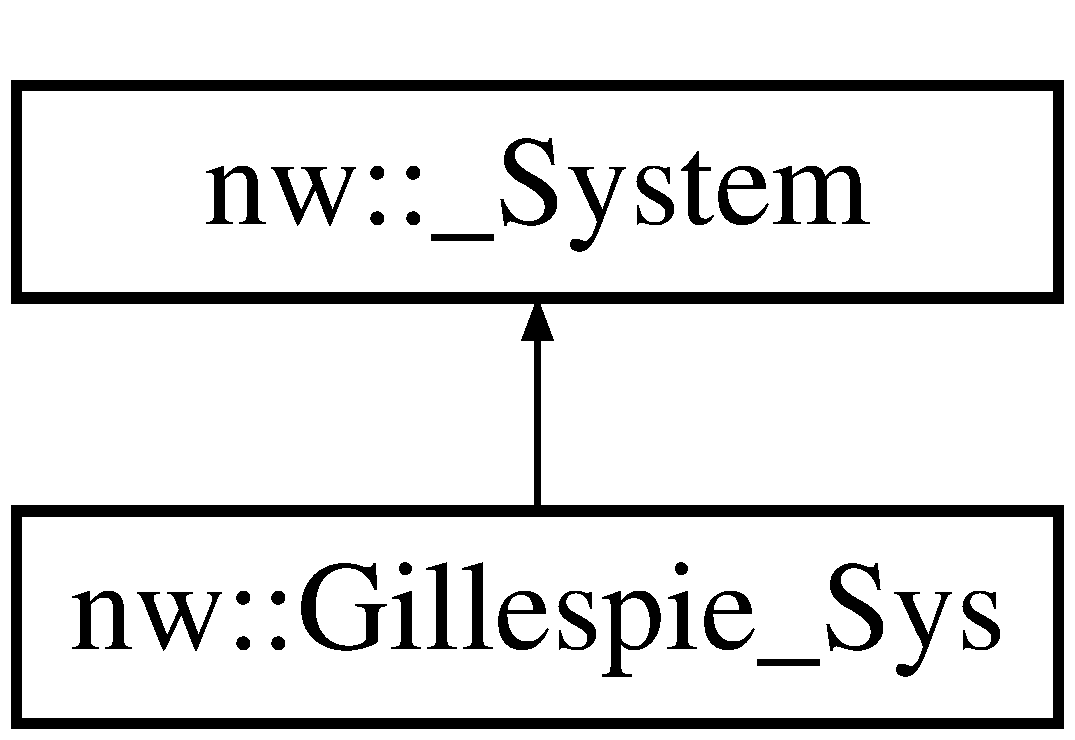
\includegraphics[height=2.000000cm]{df/d2f/classnw_1_1_gillespie___sys}
\end{center}
\end{figure}
\subsection*{Public Member Functions}
\begin{DoxyCompactItemize}
\item 
\hyperlink{classnw_1_1_gillespie___sys_aded1bb2d3c24e90b4da4e8f078b9f1b9}{Gillespie\+\_\+\+Sys} (long, long, double, double, \hyperlink{namespacenw_a0d9ea27d7802637354c7892806eac1fc}{Event\+Vector} $\ast$, \hyperlink{namespacenw_ad7146b8b5a9de9be416847f41135722c}{Voxel\+Vector} $\ast$, string, vector$<$ long $>$, vector$<$ long $>$)
\begin{DoxyCompactList}\small\item\em Constructor. \end{DoxyCompactList}\item 
virtual \hyperlink{classnw_1_1_gillespie___sys_ac1af358ef52d7a1c2e150f61e6005d6c}{$\sim$\+Gillespie\+\_\+\+Sys} ()
\begin{DoxyCompactList}\small\item\em Destructor. \end{DoxyCompactList}\item 
void \hyperlink{classnw_1_1_gillespie___sys_ad21aa35a51bac13fe64dc6d838e77aee}{go} (long)
\begin{DoxyCompactList}\small\item\em Implementation of the \hyperlink{classnw_1_1___system_ae0276aebba39a971d6e240a86a389713}{\+\_\+\+System\+::go()} method. \end{DoxyCompactList}\end{DoxyCompactItemize}
\subsection*{Private Member Functions}
\begin{DoxyCompactItemize}
\item 
void \hyperlink{classnw_1_1_gillespie___sys_a48bc0eec3fc239802276ea1499326352}{system\+\_\+output} ()
\begin{DoxyCompactList}\small\item\em file output of the system. \end{DoxyCompactList}\item 
void \hyperlink{classnw_1_1_gillespie___sys_a52f0966bbf0a561851a4e8cb52e07f51}{build\+\_\+dep\+\_\+graph} ()
\begin{DoxyCompactList}\small\item\em build the dependency graph with defined Events. \end{DoxyCompactList}\item 
void \hyperlink{classnw_1_1_gillespie___sys_afb3cc7c5515ff9646fa3ecc9c4a44e61}{print\+\_\+system\+\_\+state} ()
\begin{DoxyCompactList}\small\item\em print current \hyperlink{classnw_1_1_gillespie___sys}{Gillespie\+\_\+\+Sys} State to console \end{DoxyCompactList}\end{DoxyCompactItemize}
\subsection*{Private Attributes}
\begin{DoxyCompactItemize}
\item 
long \hyperlink{classnw_1_1_gillespie___sys_aa5b4943f29fb0276596ace75e384565e}{output\+\_\+mode}
\begin{DoxyCompactList}\small\item\em timing mode \end{DoxyCompactList}\item 
size\+\_\+t \hyperlink{classnw_1_1_gillespie___sys_a56184d8a2afdebca9cfe6e08e191fe51}{n\+\_\+steps}
\begin{DoxyCompactList}\small\item\em Holds number of simulation steps. \end{DoxyCompactList}\item 
long \hyperlink{classnw_1_1_gillespie___sys_a31f847a062a1cdc9b4a7eed103447da7}{opcntr}
\begin{DoxyCompactList}\small\item\em Output counter. \end{DoxyCompactList}\item 
long \hyperlink{classnw_1_1_gillespie___sys_a2e7300d68c9faccf444866e67842133f}{channel\+\_\+state}
\begin{DoxyCompactList}\small\item\em Tracks the channel state during the simulation to trigger the open/close timing output. \end{DoxyCompactList}\item 
double \hyperlink{classnw_1_1_gillespie___sys_a232687e1809761fea124e81aa7273f3c}{max\+\_\+\+Sim\+\_\+\+Time}
\begin{DoxyCompactList}\small\item\em Maximal simulation time. \end{DoxyCompactList}\item 
double \hyperlink{classnw_1_1_gillespie___sys_a0de156c39c87a334da7477cb2a9c02cf}{rec\+\_\+interval}
\begin{DoxyCompactList}\small\item\em Time interval, system state is recorded. \end{DoxyCompactList}\item 
double \hyperlink{classnw_1_1_gillespie___sys_ac83bb4eaee1f8b46610a8243a83fb3ad}{curr\+\_\+time}
\begin{DoxyCompactList}\small\item\em Current time. \end{DoxyCompactList}\item 
double \hyperlink{classnw_1_1_gillespie___sys_a2209a66c1cd88b06fb8a0e8b41d72b29}{rec\+\_\+time}
\begin{DoxyCompactList}\small\item\em Recording interval counter. \end{DoxyCompactList}\item 
double \hyperlink{classnw_1_1_gillespie___sys_a72cfc8f0044d7f2130f834aba5e22e18}{a\+\_\+0}
\begin{DoxyCompactList}\small\item\em Get current total system propensity a0. \end{DoxyCompactList}\item 
string \hyperlink{classnw_1_1_gillespie___sys_a07aa57de819107467a13af8ceadb4be9}{output\+\_\+dir\+\_\+path}
\begin{DoxyCompactList}\small\item\em Output directory path. \end{DoxyCompactList}\item 
stringstream \hyperlink{classnw_1_1_gillespie___sys_a989a4288ca9dd4eaf9a5ef45c805260e}{data\+\_\+path}
\begin{DoxyCompactList}\small\item\em Data output path. \end{DoxyCompactList}\item 
stringstream \hyperlink{classnw_1_1_gillespie___sys_a24b051d05da3cc35a983536371522e2c}{info\+\_\+path}
\begin{DoxyCompactList}\small\item\em Simulation info output path. \end{DoxyCompactList}\item 
stringstream \hyperlink{classnw_1_1_gillespie___sys_ab1709cadc7e452ec3834ac66a3354203}{oc\+\_\+path}
\begin{DoxyCompactList}\small\item\em Event logging output path. \end{DoxyCompactList}\item 
stringstream \hyperlink{classnw_1_1_gillespie___sys_a0d0bfd2a96ed9314b0189791d941fded}{dcol\+\_\+path}
\begin{DoxyCompactList}\small\item\em Data collection parameter path. \end{DoxyCompactList}\item 
ofstream \hyperlink{classnw_1_1_gillespie___sys_aec438472b938a410f0d31af0ae73a164}{data\+\_\+output\+\_\+file}
\begin{DoxyCompactList}\small\item\em Output file stream for simulation data output. \end{DoxyCompactList}\item 
ofstream \hyperlink{classnw_1_1_gillespie___sys_a1137e63fe12d34f81110bf5e8ebe856c}{info\+\_\+output\+\_\+file}
\begin{DoxyCompactList}\small\item\em Output file stream for simulation info output. \end{DoxyCompactList}\item 
ofstream \hyperlink{classnw_1_1_gillespie___sys_a4209e0d87ac2e0c5b9cad1074a900c80}{oc\+\_\+log\+\_\+file}
\begin{DoxyCompactList}\small\item\em Output file stream for event logging. \end{DoxyCompactList}\item 
ofstream \hyperlink{classnw_1_1_gillespie___sys_add6ed57b7c25852fab96b93b9acf9bff}{dcol\+\_\+file}
\begin{DoxyCompactList}\small\item\em Output file stream for data collection parameters. \end{DoxyCompactList}\item 
vector$<$ long $>$ \hyperlink{classnw_1_1_gillespie___sys_a98aa1c6ddc1cd3307882ef3bbf646e6a}{evt\+\_\+cntr}
\begin{DoxyCompactList}\small\item\em Counts number of Event execution. \end{DoxyCompactList}\item 
vector$<$ long $>$ \hyperlink{classnw_1_1_gillespie___sys_ae404ea4b9fea834a9c576778004fe0fe}{distr\+\_\+vec}
\begin{DoxyCompactList}\small\item\em Holds the distribution of molecular count of \hyperlink{classnw_1_1___species}{\+\_\+\+Species} with id=0. \end{DoxyCompactList}\item 
vector$<$ long $>$ \hyperlink{classnw_1_1_gillespie___sys_a138ba3dc15d538a31dbc7c1200bc5637}{osid}
\begin{DoxyCompactList}\small\item\em Output species id vector. \end{DoxyCompactList}\item 
vector$<$ long $>$ \hyperlink{classnw_1_1_gillespie___sys_a136eaaf0a00fc739e797f3b2bea22386}{ovid}
\begin{DoxyCompactList}\small\item\em Output voxel id vector. \end{DoxyCompactList}\item 
vector$<$ \hyperlink{classnw_1_1___event}{\+\_\+\+Event} $\ast$ $>$ $\ast$ \hyperlink{classnw_1_1_gillespie___sys_a3f9b4464bed7135f51413c57f086aef7}{evt\+\_\+vec}
\begin{DoxyCompactList}\small\item\em \hyperlink{classnw_1_1___event}{\+\_\+\+Event} vector \end{DoxyCompactList}\item 
vector$<$ \hyperlink{classnw_1_1___voxel}{\+\_\+\+Voxel} $\ast$ $>$ $\ast$ \hyperlink{classnw_1_1_gillespie___sys_acf4d19490ed7a8447296d7c206ef0590}{vxl\+\_\+vec}
\begin{DoxyCompactList}\small\item\em \hyperlink{classnw_1_1___voxel}{\+\_\+\+Voxel} vector \end{DoxyCompactList}\end{DoxyCompactItemize}


\subsection{Detailed Description}
Coordinates the stochastic simulation algorithm. 

The main simulation loop is defined in this class. To run the algorithm, all system relevant data structures such as the \hyperlink{classnw_1_1___event}{\+\_\+\+Event} vector (evt\+\_\+vec) and the \hyperlink{classnw_1_1___voxel}{\+\_\+\+Voxel} (vxl\+\_\+vec) vector are attributes. The whole algorithm is based on the abstract base classes that define essential properties of each system component. The polymorph approach allows for a great extensibility of these components. 

\subsection{Constructor \& Destructor Documentation}
\hypertarget{classnw_1_1_gillespie___sys_aded1bb2d3c24e90b4da4e8f078b9f1b9}{\index{nw\+::\+Gillespie\+\_\+\+Sys@{nw\+::\+Gillespie\+\_\+\+Sys}!Gillespie\+\_\+\+Sys@{Gillespie\+\_\+\+Sys}}
\index{Gillespie\+\_\+\+Sys@{Gillespie\+\_\+\+Sys}!nw\+::\+Gillespie\+\_\+\+Sys@{nw\+::\+Gillespie\+\_\+\+Sys}}
\subsubsection[{Gillespie\+\_\+\+Sys}]{\setlength{\rightskip}{0pt plus 5cm}nw\+::\+Gillespie\+\_\+\+Sys\+::\+Gillespie\+\_\+\+Sys (
\begin{DoxyParamCaption}
\item[{long}]{output\+\_\+mode, }
\item[{long}]{n\+\_\+steps, }
\item[{double}]{max\+\_\+\+Sim\+\_\+\+Time, }
\item[{double}]{rec\+\_\+interval, }
\item[{{\bf Event\+Vector} $\ast$}]{evt\+\_\+vec, }
\item[{{\bf Voxel\+Vector} $\ast$}]{vxl\+\_\+vec, }
\item[{string}]{output\+\_\+dir\+\_\+path, }
\item[{vector$<$ long $>$}]{osid, }
\item[{vector$<$ long $>$}]{ovid}
\end{DoxyParamCaption}
)}}\label{classnw_1_1_gillespie___sys_aded1bb2d3c24e90b4da4e8f078b9f1b9}


Constructor. 


\begin{DoxyParams}{Parameters}
{\em output\+\_\+mode} & Output mode \\
\hline
{\em n\+\_\+steps} & Number of simulation steps. \\
\hline
{\em max\+\_\+\+Sim\+\_\+\+Time} & Maximum simulation time. \\
\hline
{\em rec\+\_\+interval} & Time record time interval (for equidistant timeseries) \\
\hline
{\em evt\+\_\+vec} & Pointer to a vector of pointers to all defined Events. \\
\hline
{\em vxl\+\_\+vec} & Pointer to a vector of pointers to all defined Voxel. \\
\hline
{\em osid} & Output Output \hyperlink{classnw_1_1___species}{\+\_\+\+Species} Vector \\
\hline
{\em ovid} & Output Output \hyperlink{classnw_1_1___voxel}{\+\_\+\+Voxel} Vector \\
\hline
{\em output\+\_\+dir\+\_\+path} & Output Directory Path \\
\hline
\end{DoxyParams}

\begin{DoxyCode}
17                                                                  :
18     \hyperlink{classnw_1_1_gillespie___sys_aa5b4943f29fb0276596ace75e384565e}{output\_mode}(\hyperlink{classnw_1_1_gillespie___sys_aa5b4943f29fb0276596ace75e384565e}{output\_mode}),
19     \hyperlink{classnw_1_1_gillespie___sys_a56184d8a2afdebca9cfe6e08e191fe51}{n\_steps}(\hyperlink{classnw_1_1_gillespie___sys_a56184d8a2afdebca9cfe6e08e191fe51}{n\_steps}),
20     \hyperlink{classnw_1_1_gillespie___sys_a31f847a062a1cdc9b4a7eed103447da7}{opcntr}(0),
21     \hyperlink{classnw_1_1_gillespie___sys_a232687e1809761fea124e81aa7273f3c}{max\_Sim\_Time}(\hyperlink{classnw_1_1_gillespie___sys_a232687e1809761fea124e81aa7273f3c}{max\_Sim\_Time}),
22     \hyperlink{classnw_1_1_gillespie___sys_a0de156c39c87a334da7477cb2a9c02cf}{rec\_interval}(\hyperlink{classnw_1_1_gillespie___sys_a0de156c39c87a334da7477cb2a9c02cf}{rec\_interval}),
23     \hyperlink{classnw_1_1_gillespie___sys_ac83bb4eaee1f8b46610a8243a83fb3ad}{curr\_time}(0),
24     \hyperlink{classnw_1_1_gillespie___sys_a2209a66c1cd88b06fb8a0e8b41d72b29}{rec\_time}(0),
25     \hyperlink{classnw_1_1_gillespie___sys_a72cfc8f0044d7f2130f834aba5e22e18}{a\_0}(0),
26     \hyperlink{classnw_1_1_gillespie___sys_a07aa57de819107467a13af8ceadb4be9}{output\_dir\_path}(\hyperlink{classnw_1_1_gillespie___sys_a07aa57de819107467a13af8ceadb4be9}{output\_dir\_path}),
27     \hyperlink{classnw_1_1_gillespie___sys_a138ba3dc15d538a31dbc7c1200bc5637}{osid}(\hyperlink{classnw_1_1_gillespie___sys_a138ba3dc15d538a31dbc7c1200bc5637}{osid}),
28     \hyperlink{classnw_1_1_gillespie___sys_a136eaaf0a00fc739e797f3b2bea22386}{ovid}(\hyperlink{classnw_1_1_gillespie___sys_a136eaaf0a00fc739e797f3b2bea22386}{ovid}),
29     \hyperlink{classnw_1_1_gillespie___sys_a3f9b4464bed7135f51413c57f086aef7}{evt\_vec}(\hyperlink{classnw_1_1_gillespie___sys_a3f9b4464bed7135f51413c57f086aef7}{evt\_vec}),
30     \hyperlink{classnw_1_1_gillespie___sys_acf4d19490ed7a8447296d7c206ef0590}{vxl\_vec}(\hyperlink{classnw_1_1_gillespie___sys_acf4d19490ed7a8447296d7c206ef0590}{vxl\_vec})
31 \{
32 
33 \textcolor{comment}{//  initialize event counter vector}
34     \hyperlink{classnw_1_1_gillespie___sys_a98aa1c6ddc1cd3307882ef3bbf646e6a}{evt\_cntr}.assign(\hyperlink{classnw_1_1_gillespie___sys_a3f9b4464bed7135f51413c57f086aef7}{evt\_vec}->size(), 0);
35 \textcolor{comment}{//  initialize distribution vector}
36     \hyperlink{classnw_1_1_gillespie___sys_ae404ea4b9fea834a9c576778004fe0fe}{distr\_vec}.assign(500, 0);
37 
38 \textcolor{comment}{//  initialize all Events}
39     \textcolor{keywordflow}{for} (\textcolor{keywordtype}{size\_t} i = 0; i < \hyperlink{classnw_1_1_gillespie___sys_a3f9b4464bed7135f51413c57f086aef7}{evt\_vec}->size(); ++i) \{
40         \hyperlink{classnw_1_1_gillespie___sys_a3f9b4464bed7135f51413c57f086aef7}{evt\_vec}->at(i)->init();
41     \}
42 
43     this->\hyperlink{classnw_1_1_gillespie___sys_a72cfc8f0044d7f2130f834aba5e22e18}{a\_0} = 0;
44 \textcolor{comment}{//  Calculate a\_0 from all system events}
45     \textcolor{keywordflow}{for} (\textcolor{keywordtype}{size\_t} i = 0; i < this->\hyperlink{classnw_1_1_gillespie___sys_a3f9b4464bed7135f51413c57f086aef7}{evt\_vec}->size() ;++i)\{
46         this->\hyperlink{classnw_1_1_gillespie___sys_a72cfc8f0044d7f2130f834aba5e22e18}{a\_0} += this->\hyperlink{classnw_1_1_gillespie___sys_a3f9b4464bed7135f51413c57f086aef7}{evt\_vec}->at(i)->get\_a();
47     \}
48 
49 \textcolor{comment}{//  Adapt exit conditions and record interval according to the timing\_mode}
50     \textcolor{keywordflow}{if} (this->\hyperlink{classnw_1_1_gillespie___sys_aa5b4943f29fb0276596ace75e384565e}{output\_mode} == 1)\{
51         \textcolor{comment}{// set the record interval to 10 * average system waiting time}
52         this->\hyperlink{classnw_1_1_gillespie___sys_a0de156c39c87a334da7477cb2a9c02cf}{rec\_interval} = 10 / \hyperlink{classnw_1_1_gillespie___sys_a72cfc8f0044d7f2130f834aba5e22e18}{a\_0};
53     \} \textcolor{keywordflow}{else} \textcolor{keywordflow}{if} (this->\hyperlink{classnw_1_1_gillespie___sys_aa5b4943f29fb0276596ace75e384565e}{output\_mode} == 2)\{
54         this->\hyperlink{classnw_1_1_gillespie___sys_a0de156c39c87a334da7477cb2a9c02cf}{rec\_interval} = 0;
55     \}
56 
57 \textcolor{comment}{//  print data output parameters for data analysis}
58     this->\hyperlink{classnw_1_1_gillespie___sys_a0d0bfd2a96ed9314b0189791d941fded}{dcol\_path} << \hyperlink{classnw_1_1_gillespie___sys_a07aa57de819107467a13af8ceadb4be9}{output\_dir\_path} << \textcolor{stringliteral}{"sim\_param.py"};
59     \textcolor{keyword}{const} \textcolor{keywordtype}{string} &tmp\_dcol = this->\hyperlink{classnw_1_1_gillespie___sys_a0d0bfd2a96ed9314b0189791d941fded}{dcol\_path}.str();
60     this->\hyperlink{classnw_1_1_gillespie___sys_add6ed57b7c25852fab96b93b9acf9bff}{dcol\_file}.open(tmp\_dcol.c\_str());
61     this->\hyperlink{classnw_1_1_gillespie___sys_add6ed57b7c25852fab96b93b9acf9bff}{dcol\_file} << \textcolor{stringliteral}{"mean\_tau = "} << 1/this->\hyperlink{classnw_1_1_gillespie___sys_a72cfc8f0044d7f2130f834aba5e22e18}{a\_0} << endl << \textcolor{stringliteral}{"dt = "}
62                     << this->\hyperlink{classnw_1_1_gillespie___sys_a0de156c39c87a334da7477cb2a9c02cf}{rec\_interval} << endl << \textcolor{stringliteral}{"n\_steps= "} << this->
      \hyperlink{classnw_1_1_gillespie___sys_a56184d8a2afdebca9cfe6e08e191fe51}{n\_steps}
63                     << endl << \textcolor{stringliteral}{"T\_max = "} << this->\hyperlink{classnw_1_1_gillespie___sys_a232687e1809761fea124e81aa7273f3c}{max\_Sim\_Time} << endl << endl;
64     this->\hyperlink{classnw_1_1_gillespie___sys_add6ed57b7c25852fab96b93b9acf9bff}{dcol\_file}.close();
65     cout    << \textcolor{stringliteral}{"\(\backslash\)n### Timing Parameters ###\(\backslash\)n"} << \textcolor{stringliteral}{"mean\_tau = "} << 1/this->\hyperlink{classnw_1_1_gillespie___sys_a72cfc8f0044d7f2130f834aba5e22e18}{a\_0}
66             << endl << \textcolor{stringliteral}{"dt = "} << this->\hyperlink{classnw_1_1_gillespie___sys_a0de156c39c87a334da7477cb2a9c02cf}{rec\_interval} << endl << \textcolor{stringliteral}{"n\_steps= "}
67             << this->\hyperlink{classnw_1_1_gillespie___sys_a56184d8a2afdebca9cfe6e08e191fe51}{n\_steps} << endl << \textcolor{stringliteral}{"T\_max = "} << this->\hyperlink{classnw_1_1_gillespie___sys_a232687e1809761fea124e81aa7273f3c}{max\_Sim\_Time}
68             << \textcolor{stringliteral}{"\(\backslash\)n######################"} << endl << endl;
69 
70 \textcolor{comment}{//  initialize channel state log}
71     \hyperlink{classnw_1_1_gillespie___sys_a2e7300d68c9faccf444866e67842133f}{channel\_state} = 0;
72 
73 \textcolor{comment}{//  build the dependency graph}
74     \hyperlink{classnw_1_1_gillespie___sys_a52f0966bbf0a561851a4e8cb52e07f51}{build\_dep\_graph}();
75 
76 \}
\end{DoxyCode}
\hypertarget{classnw_1_1_gillespie___sys_ac1af358ef52d7a1c2e150f61e6005d6c}{\index{nw\+::\+Gillespie\+\_\+\+Sys@{nw\+::\+Gillespie\+\_\+\+Sys}!````~Gillespie\+\_\+\+Sys@{$\sim$\+Gillespie\+\_\+\+Sys}}
\index{````~Gillespie\+\_\+\+Sys@{$\sim$\+Gillespie\+\_\+\+Sys}!nw\+::\+Gillespie\+\_\+\+Sys@{nw\+::\+Gillespie\+\_\+\+Sys}}
\subsubsection[{$\sim$\+Gillespie\+\_\+\+Sys}]{\setlength{\rightskip}{0pt plus 5cm}virtual nw\+::\+Gillespie\+\_\+\+Sys\+::$\sim$\+Gillespie\+\_\+\+Sys (
\begin{DoxyParamCaption}
{}
\end{DoxyParamCaption}
)\hspace{0.3cm}{\ttfamily [inline]}, {\ttfamily [virtual]}}}\label{classnw_1_1_gillespie___sys_ac1af358ef52d7a1c2e150f61e6005d6c}


Destructor. 


\begin{DoxyCode}
47 \{\}
\end{DoxyCode}


\subsection{Member Function Documentation}
\hypertarget{classnw_1_1_gillespie___sys_a52f0966bbf0a561851a4e8cb52e07f51}{\index{nw\+::\+Gillespie\+\_\+\+Sys@{nw\+::\+Gillespie\+\_\+\+Sys}!build\+\_\+dep\+\_\+graph@{build\+\_\+dep\+\_\+graph}}
\index{build\+\_\+dep\+\_\+graph@{build\+\_\+dep\+\_\+graph}!nw\+::\+Gillespie\+\_\+\+Sys@{nw\+::\+Gillespie\+\_\+\+Sys}}
\subsubsection[{build\+\_\+dep\+\_\+graph}]{\setlength{\rightskip}{0pt plus 5cm}void nw\+::\+Gillespie\+\_\+\+Sys\+::build\+\_\+dep\+\_\+graph (
\begin{DoxyParamCaption}
{}
\end{DoxyParamCaption}
)\hspace{0.3cm}{\ttfamily [private]}}}\label{classnw_1_1_gillespie___sys_a52f0966bbf0a561851a4e8cb52e07f51}


build the dependency graph with defined Events. 

The dependency graph is an important structure for the update procedure. Through analyzing the state change vectors, dependencies are recognized and saved. All state change vectors are compared to each other. If sc\+\_\+vec a at index k is != 0 and sc\+\_\+vec b at index k is $<$ 0, b is dependent on a. 
\begin{DoxyCode}
230                                    \{
231 
232     \textcolor{keywordflow}{try}\{
233 \textcolor{comment}{//      temporary vectors}
234         vector<long> sc\_a, sc\_b;
235 
236 \textcolor{comment}{//      find dependency relations based on state change vectors}
237         \textcolor{keywordflow}{for} (\textcolor{keywordtype}{size\_t} i = 0; i < \hyperlink{classnw_1_1_gillespie___sys_a3f9b4464bed7135f51413c57f086aef7}{evt\_vec}->size(); ++i)\{
238             sc\_a = \hyperlink{classnw_1_1_gillespie___sys_a3f9b4464bed7135f51413c57f086aef7}{evt\_vec}->at(i)->get\_sc\_vec();
239             \textcolor{keywordflow}{for} (\textcolor{keywordtype}{size\_t} j = 0; j < \hyperlink{classnw_1_1_gillespie___sys_a3f9b4464bed7135f51413c57f086aef7}{evt\_vec}->size(); ++j)\{
240                 sc\_b = \hyperlink{classnw_1_1_gillespie___sys_a3f9b4464bed7135f51413c57f086aef7}{evt\_vec}->at(j)->get\_sc\_vec();
241                 \textcolor{keywordflow}{if}(\hyperlink{classnw_1_1_gillespie___sys_a3f9b4464bed7135f51413c57f086aef7}{evt\_vec}->at(i) != \hyperlink{classnw_1_1_gillespie___sys_a3f9b4464bed7135f51413c57f086aef7}{evt\_vec}->at(j))\{
242                     \textcolor{keywordflow}{for} (\textcolor{keywordtype}{size\_t} k = 0; k < sc\_a.size(); ++k)\{
243                         \textcolor{keywordflow}{if}(sc\_a.at(k) != 0 && sc\_b.at(k) < 0 )\{
244                             \hyperlink{classnw_1_1_gillespie___sys_a3f9b4464bed7135f51413c57f086aef7}{evt\_vec}->at(i)->add\_dep\_list(\hyperlink{classnw_1_1_gillespie___sys_a3f9b4464bed7135f51413c57f086aef7}{evt\_vec}->at(j));
245                             \textcolor{keywordflow}{break};
246                         \}
247                     \}
248                 \}
249             \}
250         \}
251     \}
252 
253     \textcolor{keywordflow}{catch}(exception& e)\{
254         cout << \textcolor{stringliteral}{"System::build\_dep\_graph()"} << e.what();
255     \}
256 \}
\end{DoxyCode}
\hypertarget{classnw_1_1_gillespie___sys_ad21aa35a51bac13fe64dc6d838e77aee}{\index{nw\+::\+Gillespie\+\_\+\+Sys@{nw\+::\+Gillespie\+\_\+\+Sys}!go@{go}}
\index{go@{go}!nw\+::\+Gillespie\+\_\+\+Sys@{nw\+::\+Gillespie\+\_\+\+Sys}}
\subsubsection[{go}]{\setlength{\rightskip}{0pt plus 5cm}void nw\+::\+Gillespie\+\_\+\+Sys\+::go (
\begin{DoxyParamCaption}
\item[{long}]{n\+\_\+it}
\end{DoxyParamCaption}
)\hspace{0.3cm}{\ttfamily [virtual]}}}\label{classnw_1_1_gillespie___sys_ad21aa35a51bac13fe64dc6d838e77aee}


Implementation of the \hyperlink{classnw_1_1___system_ae0276aebba39a971d6e240a86a389713}{\+\_\+\+System\+::go()} method. 


\begin{DoxyParams}{Parameters}
{\em n\+\_\+it} & Current number of simulation run (required for output file names to distinguish between multiple trajectories resulting from multiple simulation runs during one program call.)\\
\hline
\end{DoxyParams}
Start the simulation algorithm until one of the exit condition is met. The algorithm consists of the following steps\+:
\begin{DoxyEnumerate}
\item sort the event vector ascending of its tau values
\item execute first Element of the event vector
\item update all events
\item clean voxel (set dirty\+\_\+flags = {\ttfamily F\+A\+L\+S\+E})
\item loop 
\end{DoxyEnumerate}

Implements \hyperlink{classnw_1_1___system_ae0276aebba39a971d6e240a86a389713}{nw\+::\+\_\+\+System}.


\begin{DoxyCode}
80 \{
81     \textcolor{keywordflow}{try}\{
82 
83 \textcolor{comment}{//      build path to output files. n\_it represents the current simulation run.}
84 
85 \textcolor{comment}{//      data files containing molecular numbers}
86         \hyperlink{classnw_1_1_gillespie___sys_a989a4288ca9dd4eaf9a5ef45c805260e}{data\_path} << \hyperlink{classnw_1_1_gillespie___sys_a07aa57de819107467a13af8ceadb4be9}{output\_dir\_path} << \textcolor{stringliteral}{"data\_"} << n\_it << \textcolor{stringliteral}{".e"};
87 \textcolor{comment}{//      open/close log for channel dynamics}
88         \hyperlink{classnw_1_1_gillespie___sys_ab1709cadc7e452ec3834ac66a3354203}{oc\_path} << \hyperlink{classnw_1_1_gillespie___sys_a07aa57de819107467a13af8ceadb4be9}{output\_dir\_path} << \textcolor{stringliteral}{"oc\_log\_"} << n\_it << \textcolor{stringliteral}{".e"};
89 \textcolor{comment}{//      independent result log of every simulation run}
90         \hyperlink{classnw_1_1_gillespie___sys_a24b051d05da3cc35a983536371522e2c}{info\_path} << \hyperlink{classnw_1_1_gillespie___sys_a07aa57de819107467a13af8ceadb4be9}{output\_dir\_path} << \textcolor{stringliteral}{"sim\_res.e"};
91 
92         \textcolor{keyword}{const} \textcolor{keywordtype}{string} &tmp\_data = \hyperlink{classnw_1_1_gillespie___sys_a989a4288ca9dd4eaf9a5ef45c805260e}{data\_path}.str();
93         \textcolor{keyword}{const} \textcolor{keywordtype}{string} &tmp\_info = \hyperlink{classnw_1_1_gillespie___sys_a24b051d05da3cc35a983536371522e2c}{info\_path}.str();
94         \textcolor{keyword}{const} \textcolor{keywordtype}{string} &tmp\_oclog = \hyperlink{classnw_1_1_gillespie___sys_ab1709cadc7e452ec3834ac66a3354203}{oc\_path}.str();
95 
96 \textcolor{comment}{//      connect streams to output file}
97         \hyperlink{classnw_1_1_gillespie___sys_aec438472b938a410f0d31af0ae73a164}{data\_output\_file}.open(tmp\_data.c\_str());
98         \hyperlink{classnw_1_1_gillespie___sys_a4209e0d87ac2e0c5b9cad1074a900c80}{oc\_log\_file}.open(tmp\_oclog.c\_str());
99         \hyperlink{classnw_1_1_gillespie___sys_a4209e0d87ac2e0c5b9cad1074a900c80}{oc\_log\_file} << std::setprecision(10);
100 
101 \textcolor{comment}{//      reconnect to existing file (adding text)}
102         \textcolor{keywordflow}{if} (n\_it == 1)\{
103             \hyperlink{classnw_1_1_gillespie___sys_a1137e63fe12d34f81110bf5e8ebe856c}{info\_output\_file}.open(tmp\_info.c\_str());
104         \}\textcolor{keywordflow}{else}\{
105             \hyperlink{classnw_1_1_gillespie___sys_a1137e63fe12d34f81110bf5e8ebe856c}{info\_output\_file}.open(tmp\_info.c\_str(), ios::in | ios::ate);
106         \}
107 
108 \textcolor{comment}{//      console output: indicate simulation start}
109         \hyperlink{classnw_1_1_gillespie___sys_a1137e63fe12d34f81110bf5e8ebe856c}{info\_output\_file}<< \textcolor{stringliteral}{"###### Run: "} << n\_it << \textcolor{stringliteral}{" ######"} << endl;
110         cout << \textcolor{stringliteral}{"--SIMULATION BEGIN-- \(\backslash\)n"} << endl;
111         \hyperlink{classnw_1_1_gillespie___sys_a1137e63fe12d34f81110bf5e8ebe856c}{info\_output\_file} << \textcolor{stringliteral}{"--SIMULATION RESULTS-- \(\backslash\)n"} << endl;
112 
113 \textcolor{comment}{//      print the initial system state}
114         \hyperlink{classnw_1_1_gillespie___sys_afb3cc7c5515ff9646fa3ecc9c4a44e61}{print\_system\_state}();
115 
116 \textcolor{comment}{//      ###############################}
117 \textcolor{comment}{//      ## START THE SIMULATION LOOP ##}
118 \textcolor{comment}{//      ###############################}
119 
120 \textcolor{comment}{//      set times}
121         \textcolor{keywordtype}{double} tau = 0, begin, end;
122         begin = time(0);
123 
124 \textcolor{comment}{//      check exit conditions}
125         \textcolor{keywordflow}{for} (\textcolor{keywordtype}{size\_t} i = 0; i < \hyperlink{classnw_1_1_gillespie___sys_a56184d8a2afdebca9cfe6e08e191fe51}{n\_steps}; ++i) \{
126             \textcolor{keywordflow}{if} (\hyperlink{classnw_1_1_gillespie___sys_ac83bb4eaee1f8b46610a8243a83fb3ad}{curr\_time} <= \hyperlink{classnw_1_1_gillespie___sys_a232687e1809761fea124e81aa7273f3c}{max\_Sim\_Time}) \{
127 
128                 \textcolor{keywordtype}{long} nextIndex = 0;
129                 \textcolor{keywordtype}{double} minTau = INFINITY;
130 
131 \textcolor{comment}{//              event update procedure}
132                 \textcolor{keywordflow}{for} (\textcolor{keywordtype}{size\_t} j = 0; j < \hyperlink{classnw_1_1_gillespie___sys_a3f9b4464bed7135f51413c57f086aef7}{evt\_vec}->size(); ++j) \{
133                     \textcolor{keywordtype}{double} actTau = \hyperlink{classnw_1_1_gillespie___sys_a3f9b4464bed7135f51413c57f086aef7}{evt\_vec}->at(j)->update(tau);
134 \textcolor{comment}{//                  determine next Event Index}
135                     \textcolor{keywordflow}{if} (actTau < minTau) \{
136                         minTau = actTau;
137                         nextIndex = j;
138                     \}
139                 \}
140 
141 \textcolor{comment}{//              update system times}
142                 tau = minTau;
143                 \hyperlink{classnw_1_1_gillespie___sys_a2209a66c1cd88b06fb8a0e8b41d72b29}{rec\_time} += tau;
144                 \hyperlink{classnw_1_1_gillespie___sys_ac83bb4eaee1f8b46610a8243a83fb3ad}{curr\_time} += tau;
145 
146 \textcolor{comment}{//              update event counter}
147                 \hyperlink{classnw_1_1_gillespie___sys_a98aa1c6ddc1cd3307882ef3bbf646e6a}{evt\_cntr}[nextIndex]++;
148 
149 \textcolor{comment}{//              execute next Event}
150                 \hyperlink{classnw_1_1_gillespie___sys_a3f9b4464bed7135f51413c57f086aef7}{evt\_vec}->at(nextIndex)->execute();
151 
152 \textcolor{comment}{//              print system state if necessary}
153                 \hyperlink{classnw_1_1_gillespie___sys_a48bc0eec3fc239802276ea1499326352}{system\_output}();
154 
155             \} \textcolor{keywordflow}{else}\{
156                 n\_steps = i;
157                 \textcolor{keywordflow}{break};
158             \}
159         \}
160 
161 \textcolor{comment}{//      ############################}
162 \textcolor{comment}{//      ## END OF SIMULATION LOOP ##}
163 \textcolor{comment}{//      ############################}
164 
165         end = time(0);
166 
167 \textcolor{comment}{//      output of event distribution in info\_output\_file}
168         cout << \textcolor{stringliteral}{"Event distribution:\(\backslash\)t"};
169         \hyperlink{classnw_1_1_gillespie___sys_a1137e63fe12d34f81110bf5e8ebe856c}{info\_output\_file} << \textcolor{stringliteral}{"Event distribution:\(\backslash\)t"};
170         \textcolor{keywordflow}{for} (\textcolor{keywordtype}{long} p = 0; p < (long)\hyperlink{classnw_1_1_gillespie___sys_a98aa1c6ddc1cd3307882ef3bbf646e6a}{evt\_cntr}.size(); p++)\{
171             cout << \hyperlink{classnw_1_1_gillespie___sys_a98aa1c6ddc1cd3307882ef3bbf646e6a}{evt\_cntr}.at(p) << \textcolor{stringliteral}{","};
172             \hyperlink{classnw_1_1_gillespie___sys_a1137e63fe12d34f81110bf5e8ebe856c}{info\_output\_file} << \hyperlink{classnw_1_1_gillespie___sys_a98aa1c6ddc1cd3307882ef3bbf646e6a}{evt\_cntr}.at(p) << \textcolor{stringliteral}{","};
173         \}
174         cout << endl;
175         \hyperlink{classnw_1_1_gillespie___sys_a1137e63fe12d34f81110bf5e8ebe856c}{info\_output\_file} << endl;
176 
177 \textcolor{comment}{//      system information output to info\_output\_file.}
178         cout << \textcolor{stringliteral}{"Simulated time:\(\backslash\)t\(\backslash\)t"} << \hyperlink{classnw_1_1_gillespie___sys_ac83bb4eaee1f8b46610a8243a83fb3ad}{curr\_time} << \textcolor{stringliteral}{" ms"} << endl;
179         \hyperlink{classnw_1_1_gillespie___sys_a1137e63fe12d34f81110bf5e8ebe856c}{info\_output\_file} << \textcolor{stringliteral}{"Simulated time:\(\backslash\)t\(\backslash\)t"} << \hyperlink{classnw_1_1_gillespie___sys_ac83bb4eaee1f8b46610a8243a83fb3ad}{curr\_time} << \textcolor{stringliteral}{" ms"} << endl;
180         cout << \textcolor{stringliteral}{"Number of steps: \(\backslash\)t"} << n\_steps << endl;
181         \hyperlink{classnw_1_1_gillespie___sys_a1137e63fe12d34f81110bf5e8ebe856c}{info\_output\_file} << \textcolor{stringliteral}{"Number of steps: \(\backslash\)t"} << n\_steps << endl;
182         cout << \textcolor{stringliteral}{"Computation time:\(\backslash\)t"} << end - begin << \textcolor{stringliteral}{" s"} << endl;
183         \hyperlink{classnw_1_1_gillespie___sys_a1137e63fe12d34f81110bf5e8ebe856c}{info\_output\_file} << \textcolor{stringliteral}{"Computation time:\(\backslash\)t"} << end - begin << \textcolor{stringliteral}{" s"} << endl;
184 
185 \textcolor{comment}{//      console output: indicate simulation end}
186         \hyperlink{classnw_1_1_gillespie___sys_afb3cc7c5515ff9646fa3ecc9c4a44e61}{print\_system\_state}();
187         cout << \textcolor{stringliteral}{"\(\backslash\)n--SIMULATION END--"} << endl;
188         \hyperlink{classnw_1_1_gillespie___sys_a1137e63fe12d34f81110bf5e8ebe856c}{info\_output\_file} << \textcolor{stringliteral}{"\(\backslash\)n--SIMULATION END--"} << endl << endl << endl;
189 
190 \textcolor{comment}{//      disconnect stream from output file}
191         \hyperlink{classnw_1_1_gillespie___sys_aec438472b938a410f0d31af0ae73a164}{data\_output\_file}.close();
192         \hyperlink{classnw_1_1_gillespie___sys_a1137e63fe12d34f81110bf5e8ebe856c}{info\_output\_file}.close();
193         \hyperlink{classnw_1_1_gillespie___sys_a4209e0d87ac2e0c5b9cad1074a900c80}{oc\_log\_file}.close();
194     \}
195 
196     \textcolor{keywordflow}{catch}(exception& e)\{
197         cout << \textcolor{stringliteral}{"System::go(): "} << e.what() << endl;
198     \}
199 \}
\end{DoxyCode}
\hypertarget{classnw_1_1_gillespie___sys_afb3cc7c5515ff9646fa3ecc9c4a44e61}{\index{nw\+::\+Gillespie\+\_\+\+Sys@{nw\+::\+Gillespie\+\_\+\+Sys}!print\+\_\+system\+\_\+state@{print\+\_\+system\+\_\+state}}
\index{print\+\_\+system\+\_\+state@{print\+\_\+system\+\_\+state}!nw\+::\+Gillespie\+\_\+\+Sys@{nw\+::\+Gillespie\+\_\+\+Sys}}
\subsubsection[{print\+\_\+system\+\_\+state}]{\setlength{\rightskip}{0pt plus 5cm}void nw\+::\+Gillespie\+\_\+\+Sys\+::print\+\_\+system\+\_\+state (
\begin{DoxyParamCaption}
{}
\end{DoxyParamCaption}
)\hspace{0.3cm}{\ttfamily [private]}}}\label{classnw_1_1_gillespie___sys_afb3cc7c5515ff9646fa3ecc9c4a44e61}


print current \hyperlink{classnw_1_1_gillespie___sys}{Gillespie\+\_\+\+Sys} State to console 


\begin{DoxyCode}
258                                       \{
259 
260 \textcolor{comment}{//  print current system state}
261     cout << \textcolor{stringliteral}{"---System State---\(\backslash\)n"};
262     \hyperlink{classnw_1_1_gillespie___sys_a1137e63fe12d34f81110bf5e8ebe856c}{info\_output\_file} << \textcolor{stringliteral}{"---System State---\(\backslash\)n"};
263     \textcolor{keywordflow}{for} (\textcolor{keywordtype}{long} i = 0; i < (long)\hyperlink{classnw_1_1_gillespie___sys_acf4d19490ed7a8447296d7c206ef0590}{vxl\_vec}->size();i++)\{
264         cout << \textcolor{stringliteral}{"Voxel "} << i << \textcolor{stringliteral}{": "};
265         \hyperlink{classnw_1_1_gillespie___sys_a1137e63fe12d34f81110bf5e8ebe856c}{info\_output\_file} << \textcolor{stringliteral}{"Voxel "} << i << \textcolor{stringliteral}{": "};
266         \textcolor{keywordflow}{for} (\textcolor{keywordtype}{long} j = 0; j < (long)\hyperlink{classnw_1_1_gillespie___sys_acf4d19490ed7a8447296d7c206ef0590}{vxl\_vec}->at(i)->get\_state\_vec()->size(); j++)\{
267             cout << \hyperlink{classnw_1_1_gillespie___sys_acf4d19490ed7a8447296d7c206ef0590}{vxl\_vec}->at(i)->get\_state\_vec()->at(j)->get\_n\_molecules() << \textcolor{stringliteral}{","};
268             \hyperlink{classnw_1_1_gillespie___sys_a1137e63fe12d34f81110bf5e8ebe856c}{info\_output\_file} << \hyperlink{classnw_1_1_gillespie___sys_acf4d19490ed7a8447296d7c206ef0590}{vxl\_vec}->at(i)->get\_state\_vec()->at(j)->
      get\_n\_molecules() << \textcolor{stringliteral}{","};
269         \}
270         cout << endl;
271         \hyperlink{classnw_1_1_gillespie___sys_a1137e63fe12d34f81110bf5e8ebe856c}{info\_output\_file} << endl;
272     \}
273     cout << \textcolor{stringliteral}{"------------------\(\backslash\)n"};
274     \hyperlink{classnw_1_1_gillespie___sys_a1137e63fe12d34f81110bf5e8ebe856c}{info\_output\_file} << \textcolor{stringliteral}{"------------------\(\backslash\)n"};
275 \}
\end{DoxyCode}
\hypertarget{classnw_1_1_gillespie___sys_a48bc0eec3fc239802276ea1499326352}{\index{nw\+::\+Gillespie\+\_\+\+Sys@{nw\+::\+Gillespie\+\_\+\+Sys}!system\+\_\+output@{system\+\_\+output}}
\index{system\+\_\+output@{system\+\_\+output}!nw\+::\+Gillespie\+\_\+\+Sys@{nw\+::\+Gillespie\+\_\+\+Sys}}
\subsubsection[{system\+\_\+output}]{\setlength{\rightskip}{0pt plus 5cm}void nw\+::\+Gillespie\+\_\+\+Sys\+::system\+\_\+output (
\begin{DoxyParamCaption}
{}
\end{DoxyParamCaption}
)\hspace{0.3cm}{\ttfamily [inline]}, {\ttfamily [private]}}}\label{classnw_1_1_gillespie___sys_a48bc0eec3fc239802276ea1499326352}


file output of the system. 

The function \hyperlink{classnw_1_1_gillespie___sys_a48bc0eec3fc239802276ea1499326352}{system\+\_\+output()} takes care, that the a predefined part (input file) of the system state is recorded with a discrete record interval. 
\begin{DoxyCode}
201                                         \{
202 \textcolor{comment}{//  print system state with a fixed time step dt (recording interval)}
203     \textcolor{keywordflow}{if} (\hyperlink{classnw_1_1_gillespie___sys_a2209a66c1cd88b06fb8a0e8b41d72b29}{rec\_time} >= \hyperlink{classnw_1_1_gillespie___sys_a0de156c39c87a334da7477cb2a9c02cf}{rec\_interval})\{
204 \textcolor{comment}{//          run through output voxel vector}
205             \textcolor{keywordflow}{for}(\textcolor{keywordtype}{size\_t} k = 0; k < \hyperlink{classnw_1_1_gillespie___sys_a136eaaf0a00fc739e797f3b2bea22386}{ovid}.size(); ++k)\{
206 \textcolor{comment}{//              run through output species id vector}
207                 \textcolor{keywordflow}{for}(\textcolor{keywordtype}{size\_t} i = 0; i < \hyperlink{classnw_1_1_gillespie___sys_a138ba3dc15d538a31dbc7c1200bc5637}{osid}.size(); ++i)\{
208                     \hyperlink{classnw_1_1_gillespie___sys_aec438472b938a410f0d31af0ae73a164}{data\_output\_file}<<  \hyperlink{classnw_1_1_gillespie___sys_acf4d19490ed7a8447296d7c206ef0590}{vxl\_vec}->at(\hyperlink{classnw_1_1_gillespie___sys_a136eaaf0a00fc739e797f3b2bea22386}{ovid}[k])->get\_state\_vec()
209                                         ->at(\hyperlink{classnw_1_1_gillespie___sys_a138ba3dc15d538a31dbc7c1200bc5637}{osid}[i])->get\_n\_molecules() << \textcolor{stringliteral}{","};
210                 \}
211             \}
212         \textcolor{keywordflow}{if} (this->\hyperlink{classnw_1_1_gillespie___sys_aa5b4943f29fb0276596ace75e384565e}{output\_mode} == 2)\{
213             \hyperlink{classnw_1_1_gillespie___sys_aec438472b938a410f0d31af0ae73a164}{data\_output\_file} << \hyperlink{classnw_1_1_gillespie___sys_ac83bb4eaee1f8b46610a8243a83fb3ad}{curr\_time} << \textcolor{stringliteral}{","};
214         \}
215         \hyperlink{classnw_1_1_gillespie___sys_a31f847a062a1cdc9b4a7eed103447da7}{opcntr}++;
216         \hyperlink{classnw_1_1_gillespie___sys_a2209a66c1cd88b06fb8a0e8b41d72b29}{rec\_time} -= \hyperlink{classnw_1_1_gillespie___sys_a0de156c39c87a334da7477cb2a9c02cf}{rec\_interval};
217     \}
218 
219 \textcolor{comment}{//  check if the channel state changed and if so log the open and close times}
220     \textcolor{keywordflow}{if}( \hyperlink{classnw_1_1_gillespie___sys_acf4d19490ed7a8447296d7c206ef0590}{vxl\_vec}->at(0)->get\_state\_vec()->at(\hyperlink{classnw_1_1_gillespie___sys_acf4d19490ed7a8447296d7c206ef0590}{vxl\_vec}->at(0)
221         ->get\_state\_vec()->size()-1)->get\_n\_molecules() != \hyperlink{classnw_1_1_gillespie___sys_a2e7300d68c9faccf444866e67842133f}{channel\_state})\{
222 \textcolor{comment}{//      update current channel state}
223         \hyperlink{classnw_1_1_gillespie___sys_a2e7300d68c9faccf444866e67842133f}{channel\_state} = \hyperlink{classnw_1_1_gillespie___sys_acf4d19490ed7a8447296d7c206ef0590}{vxl\_vec}->at(0)->get\_state\_vec()->at(
      \hyperlink{classnw_1_1_gillespie___sys_acf4d19490ed7a8447296d7c206ef0590}{vxl\_vec}->at(0)
224                         ->get\_state\_vec()->size() - 1)->get\_n\_molecules();
225 \textcolor{comment}{//      write current system time to oc\_log.e}
226         \hyperlink{classnw_1_1_gillespie___sys_a4209e0d87ac2e0c5b9cad1074a900c80}{oc\_log\_file} << \hyperlink{classnw_1_1_gillespie___sys_ac83bb4eaee1f8b46610a8243a83fb3ad}{curr\_time} << \textcolor{stringliteral}{","};
227     \}
228 \}
\end{DoxyCode}


\subsection{Member Data Documentation}
\hypertarget{classnw_1_1_gillespie___sys_a72cfc8f0044d7f2130f834aba5e22e18}{\index{nw\+::\+Gillespie\+\_\+\+Sys@{nw\+::\+Gillespie\+\_\+\+Sys}!a\+\_\+0@{a\+\_\+0}}
\index{a\+\_\+0@{a\+\_\+0}!nw\+::\+Gillespie\+\_\+\+Sys@{nw\+::\+Gillespie\+\_\+\+Sys}}
\subsubsection[{a\+\_\+0}]{\setlength{\rightskip}{0pt plus 5cm}double nw\+::\+Gillespie\+\_\+\+Sys\+::a\+\_\+0\hspace{0.3cm}{\ttfamily [private]}}}\label{classnw_1_1_gillespie___sys_a72cfc8f0044d7f2130f834aba5e22e18}


Get current total system propensity a0. 

\hypertarget{classnw_1_1_gillespie___sys_a2e7300d68c9faccf444866e67842133f}{\index{nw\+::\+Gillespie\+\_\+\+Sys@{nw\+::\+Gillespie\+\_\+\+Sys}!channel\+\_\+state@{channel\+\_\+state}}
\index{channel\+\_\+state@{channel\+\_\+state}!nw\+::\+Gillespie\+\_\+\+Sys@{nw\+::\+Gillespie\+\_\+\+Sys}}
\subsubsection[{channel\+\_\+state}]{\setlength{\rightskip}{0pt plus 5cm}long nw\+::\+Gillespie\+\_\+\+Sys\+::channel\+\_\+state\hspace{0.3cm}{\ttfamily [private]}}}\label{classnw_1_1_gillespie___sys_a2e7300d68c9faccf444866e67842133f}


Tracks the channel state during the simulation to trigger the open/close timing output. 

\hypertarget{classnw_1_1_gillespie___sys_ac83bb4eaee1f8b46610a8243a83fb3ad}{\index{nw\+::\+Gillespie\+\_\+\+Sys@{nw\+::\+Gillespie\+\_\+\+Sys}!curr\+\_\+time@{curr\+\_\+time}}
\index{curr\+\_\+time@{curr\+\_\+time}!nw\+::\+Gillespie\+\_\+\+Sys@{nw\+::\+Gillespie\+\_\+\+Sys}}
\subsubsection[{curr\+\_\+time}]{\setlength{\rightskip}{0pt plus 5cm}double nw\+::\+Gillespie\+\_\+\+Sys\+::curr\+\_\+time\hspace{0.3cm}{\ttfamily [private]}}}\label{classnw_1_1_gillespie___sys_ac83bb4eaee1f8b46610a8243a83fb3ad}


Current time. 

\hypertarget{classnw_1_1_gillespie___sys_aec438472b938a410f0d31af0ae73a164}{\index{nw\+::\+Gillespie\+\_\+\+Sys@{nw\+::\+Gillespie\+\_\+\+Sys}!data\+\_\+output\+\_\+file@{data\+\_\+output\+\_\+file}}
\index{data\+\_\+output\+\_\+file@{data\+\_\+output\+\_\+file}!nw\+::\+Gillespie\+\_\+\+Sys@{nw\+::\+Gillespie\+\_\+\+Sys}}
\subsubsection[{data\+\_\+output\+\_\+file}]{\setlength{\rightskip}{0pt plus 5cm}ofstream nw\+::\+Gillespie\+\_\+\+Sys\+::data\+\_\+output\+\_\+file\hspace{0.3cm}{\ttfamily [private]}}}\label{classnw_1_1_gillespie___sys_aec438472b938a410f0d31af0ae73a164}


Output file stream for simulation data output. 

\hypertarget{classnw_1_1_gillespie___sys_a989a4288ca9dd4eaf9a5ef45c805260e}{\index{nw\+::\+Gillespie\+\_\+\+Sys@{nw\+::\+Gillespie\+\_\+\+Sys}!data\+\_\+path@{data\+\_\+path}}
\index{data\+\_\+path@{data\+\_\+path}!nw\+::\+Gillespie\+\_\+\+Sys@{nw\+::\+Gillespie\+\_\+\+Sys}}
\subsubsection[{data\+\_\+path}]{\setlength{\rightskip}{0pt plus 5cm}stringstream nw\+::\+Gillespie\+\_\+\+Sys\+::data\+\_\+path\hspace{0.3cm}{\ttfamily [private]}}}\label{classnw_1_1_gillespie___sys_a989a4288ca9dd4eaf9a5ef45c805260e}


Data output path. 

\hypertarget{classnw_1_1_gillespie___sys_add6ed57b7c25852fab96b93b9acf9bff}{\index{nw\+::\+Gillespie\+\_\+\+Sys@{nw\+::\+Gillespie\+\_\+\+Sys}!dcol\+\_\+file@{dcol\+\_\+file}}
\index{dcol\+\_\+file@{dcol\+\_\+file}!nw\+::\+Gillespie\+\_\+\+Sys@{nw\+::\+Gillespie\+\_\+\+Sys}}
\subsubsection[{dcol\+\_\+file}]{\setlength{\rightskip}{0pt plus 5cm}ofstream nw\+::\+Gillespie\+\_\+\+Sys\+::dcol\+\_\+file\hspace{0.3cm}{\ttfamily [private]}}}\label{classnw_1_1_gillespie___sys_add6ed57b7c25852fab96b93b9acf9bff}


Output file stream for data collection parameters. 

\hypertarget{classnw_1_1_gillespie___sys_a0d0bfd2a96ed9314b0189791d941fded}{\index{nw\+::\+Gillespie\+\_\+\+Sys@{nw\+::\+Gillespie\+\_\+\+Sys}!dcol\+\_\+path@{dcol\+\_\+path}}
\index{dcol\+\_\+path@{dcol\+\_\+path}!nw\+::\+Gillespie\+\_\+\+Sys@{nw\+::\+Gillespie\+\_\+\+Sys}}
\subsubsection[{dcol\+\_\+path}]{\setlength{\rightskip}{0pt plus 5cm}stringstream nw\+::\+Gillespie\+\_\+\+Sys\+::dcol\+\_\+path\hspace{0.3cm}{\ttfamily [private]}}}\label{classnw_1_1_gillespie___sys_a0d0bfd2a96ed9314b0189791d941fded}


Data collection parameter path. 

\hypertarget{classnw_1_1_gillespie___sys_ae404ea4b9fea834a9c576778004fe0fe}{\index{nw\+::\+Gillespie\+\_\+\+Sys@{nw\+::\+Gillespie\+\_\+\+Sys}!distr\+\_\+vec@{distr\+\_\+vec}}
\index{distr\+\_\+vec@{distr\+\_\+vec}!nw\+::\+Gillespie\+\_\+\+Sys@{nw\+::\+Gillespie\+\_\+\+Sys}}
\subsubsection[{distr\+\_\+vec}]{\setlength{\rightskip}{0pt plus 5cm}vector$<$long$>$ nw\+::\+Gillespie\+\_\+\+Sys\+::distr\+\_\+vec\hspace{0.3cm}{\ttfamily [private]}}}\label{classnw_1_1_gillespie___sys_ae404ea4b9fea834a9c576778004fe0fe}


Holds the distribution of molecular count of \hyperlink{classnw_1_1___species}{\+\_\+\+Species} with id=0. 

\hypertarget{classnw_1_1_gillespie___sys_a98aa1c6ddc1cd3307882ef3bbf646e6a}{\index{nw\+::\+Gillespie\+\_\+\+Sys@{nw\+::\+Gillespie\+\_\+\+Sys}!evt\+\_\+cntr@{evt\+\_\+cntr}}
\index{evt\+\_\+cntr@{evt\+\_\+cntr}!nw\+::\+Gillespie\+\_\+\+Sys@{nw\+::\+Gillespie\+\_\+\+Sys}}
\subsubsection[{evt\+\_\+cntr}]{\setlength{\rightskip}{0pt plus 5cm}vector$<$long$>$ nw\+::\+Gillespie\+\_\+\+Sys\+::evt\+\_\+cntr\hspace{0.3cm}{\ttfamily [private]}}}\label{classnw_1_1_gillespie___sys_a98aa1c6ddc1cd3307882ef3bbf646e6a}


Counts number of Event execution. 

\hypertarget{classnw_1_1_gillespie___sys_a3f9b4464bed7135f51413c57f086aef7}{\index{nw\+::\+Gillespie\+\_\+\+Sys@{nw\+::\+Gillespie\+\_\+\+Sys}!evt\+\_\+vec@{evt\+\_\+vec}}
\index{evt\+\_\+vec@{evt\+\_\+vec}!nw\+::\+Gillespie\+\_\+\+Sys@{nw\+::\+Gillespie\+\_\+\+Sys}}
\subsubsection[{evt\+\_\+vec}]{\setlength{\rightskip}{0pt plus 5cm}vector$<${\bf \+\_\+\+Event}$\ast$$>$$\ast$ nw\+::\+Gillespie\+\_\+\+Sys\+::evt\+\_\+vec\hspace{0.3cm}{\ttfamily [private]}}}\label{classnw_1_1_gillespie___sys_a3f9b4464bed7135f51413c57f086aef7}


\hyperlink{classnw_1_1___event}{\+\_\+\+Event} vector 

\hypertarget{classnw_1_1_gillespie___sys_a1137e63fe12d34f81110bf5e8ebe856c}{\index{nw\+::\+Gillespie\+\_\+\+Sys@{nw\+::\+Gillespie\+\_\+\+Sys}!info\+\_\+output\+\_\+file@{info\+\_\+output\+\_\+file}}
\index{info\+\_\+output\+\_\+file@{info\+\_\+output\+\_\+file}!nw\+::\+Gillespie\+\_\+\+Sys@{nw\+::\+Gillespie\+\_\+\+Sys}}
\subsubsection[{info\+\_\+output\+\_\+file}]{\setlength{\rightskip}{0pt plus 5cm}ofstream nw\+::\+Gillespie\+\_\+\+Sys\+::info\+\_\+output\+\_\+file\hspace{0.3cm}{\ttfamily [private]}}}\label{classnw_1_1_gillespie___sys_a1137e63fe12d34f81110bf5e8ebe856c}


Output file stream for simulation info output. 

\hypertarget{classnw_1_1_gillespie___sys_a24b051d05da3cc35a983536371522e2c}{\index{nw\+::\+Gillespie\+\_\+\+Sys@{nw\+::\+Gillespie\+\_\+\+Sys}!info\+\_\+path@{info\+\_\+path}}
\index{info\+\_\+path@{info\+\_\+path}!nw\+::\+Gillespie\+\_\+\+Sys@{nw\+::\+Gillespie\+\_\+\+Sys}}
\subsubsection[{info\+\_\+path}]{\setlength{\rightskip}{0pt plus 5cm}stringstream nw\+::\+Gillespie\+\_\+\+Sys\+::info\+\_\+path\hspace{0.3cm}{\ttfamily [private]}}}\label{classnw_1_1_gillespie___sys_a24b051d05da3cc35a983536371522e2c}


Simulation info output path. 

\hypertarget{classnw_1_1_gillespie___sys_a232687e1809761fea124e81aa7273f3c}{\index{nw\+::\+Gillespie\+\_\+\+Sys@{nw\+::\+Gillespie\+\_\+\+Sys}!max\+\_\+\+Sim\+\_\+\+Time@{max\+\_\+\+Sim\+\_\+\+Time}}
\index{max\+\_\+\+Sim\+\_\+\+Time@{max\+\_\+\+Sim\+\_\+\+Time}!nw\+::\+Gillespie\+\_\+\+Sys@{nw\+::\+Gillespie\+\_\+\+Sys}}
\subsubsection[{max\+\_\+\+Sim\+\_\+\+Time}]{\setlength{\rightskip}{0pt plus 5cm}double nw\+::\+Gillespie\+\_\+\+Sys\+::max\+\_\+\+Sim\+\_\+\+Time\hspace{0.3cm}{\ttfamily [private]}}}\label{classnw_1_1_gillespie___sys_a232687e1809761fea124e81aa7273f3c}


Maximal simulation time. 

\hypertarget{classnw_1_1_gillespie___sys_a56184d8a2afdebca9cfe6e08e191fe51}{\index{nw\+::\+Gillespie\+\_\+\+Sys@{nw\+::\+Gillespie\+\_\+\+Sys}!n\+\_\+steps@{n\+\_\+steps}}
\index{n\+\_\+steps@{n\+\_\+steps}!nw\+::\+Gillespie\+\_\+\+Sys@{nw\+::\+Gillespie\+\_\+\+Sys}}
\subsubsection[{n\+\_\+steps}]{\setlength{\rightskip}{0pt plus 5cm}size\+\_\+t nw\+::\+Gillespie\+\_\+\+Sys\+::n\+\_\+steps\hspace{0.3cm}{\ttfamily [private]}}}\label{classnw_1_1_gillespie___sys_a56184d8a2afdebca9cfe6e08e191fe51}


Holds number of simulation steps. 

\hypertarget{classnw_1_1_gillespie___sys_a4209e0d87ac2e0c5b9cad1074a900c80}{\index{nw\+::\+Gillespie\+\_\+\+Sys@{nw\+::\+Gillespie\+\_\+\+Sys}!oc\+\_\+log\+\_\+file@{oc\+\_\+log\+\_\+file}}
\index{oc\+\_\+log\+\_\+file@{oc\+\_\+log\+\_\+file}!nw\+::\+Gillespie\+\_\+\+Sys@{nw\+::\+Gillespie\+\_\+\+Sys}}
\subsubsection[{oc\+\_\+log\+\_\+file}]{\setlength{\rightskip}{0pt plus 5cm}ofstream nw\+::\+Gillespie\+\_\+\+Sys\+::oc\+\_\+log\+\_\+file\hspace{0.3cm}{\ttfamily [private]}}}\label{classnw_1_1_gillespie___sys_a4209e0d87ac2e0c5b9cad1074a900c80}


Output file stream for event logging. 

\hypertarget{classnw_1_1_gillespie___sys_ab1709cadc7e452ec3834ac66a3354203}{\index{nw\+::\+Gillespie\+\_\+\+Sys@{nw\+::\+Gillespie\+\_\+\+Sys}!oc\+\_\+path@{oc\+\_\+path}}
\index{oc\+\_\+path@{oc\+\_\+path}!nw\+::\+Gillespie\+\_\+\+Sys@{nw\+::\+Gillespie\+\_\+\+Sys}}
\subsubsection[{oc\+\_\+path}]{\setlength{\rightskip}{0pt plus 5cm}stringstream nw\+::\+Gillespie\+\_\+\+Sys\+::oc\+\_\+path\hspace{0.3cm}{\ttfamily [private]}}}\label{classnw_1_1_gillespie___sys_ab1709cadc7e452ec3834ac66a3354203}


Event logging output path. 

\hypertarget{classnw_1_1_gillespie___sys_a31f847a062a1cdc9b4a7eed103447da7}{\index{nw\+::\+Gillespie\+\_\+\+Sys@{nw\+::\+Gillespie\+\_\+\+Sys}!opcntr@{opcntr}}
\index{opcntr@{opcntr}!nw\+::\+Gillespie\+\_\+\+Sys@{nw\+::\+Gillespie\+\_\+\+Sys}}
\subsubsection[{opcntr}]{\setlength{\rightskip}{0pt plus 5cm}long nw\+::\+Gillespie\+\_\+\+Sys\+::opcntr\hspace{0.3cm}{\ttfamily [private]}}}\label{classnw_1_1_gillespie___sys_a31f847a062a1cdc9b4a7eed103447da7}


Output counter. 

\hypertarget{classnw_1_1_gillespie___sys_a138ba3dc15d538a31dbc7c1200bc5637}{\index{nw\+::\+Gillespie\+\_\+\+Sys@{nw\+::\+Gillespie\+\_\+\+Sys}!osid@{osid}}
\index{osid@{osid}!nw\+::\+Gillespie\+\_\+\+Sys@{nw\+::\+Gillespie\+\_\+\+Sys}}
\subsubsection[{osid}]{\setlength{\rightskip}{0pt plus 5cm}vector$<$long$>$ nw\+::\+Gillespie\+\_\+\+Sys\+::osid\hspace{0.3cm}{\ttfamily [private]}}}\label{classnw_1_1_gillespie___sys_a138ba3dc15d538a31dbc7c1200bc5637}


Output species id vector. 

\hypertarget{classnw_1_1_gillespie___sys_a07aa57de819107467a13af8ceadb4be9}{\index{nw\+::\+Gillespie\+\_\+\+Sys@{nw\+::\+Gillespie\+\_\+\+Sys}!output\+\_\+dir\+\_\+path@{output\+\_\+dir\+\_\+path}}
\index{output\+\_\+dir\+\_\+path@{output\+\_\+dir\+\_\+path}!nw\+::\+Gillespie\+\_\+\+Sys@{nw\+::\+Gillespie\+\_\+\+Sys}}
\subsubsection[{output\+\_\+dir\+\_\+path}]{\setlength{\rightskip}{0pt plus 5cm}string nw\+::\+Gillespie\+\_\+\+Sys\+::output\+\_\+dir\+\_\+path\hspace{0.3cm}{\ttfamily [private]}}}\label{classnw_1_1_gillespie___sys_a07aa57de819107467a13af8ceadb4be9}


Output directory path. 

\hypertarget{classnw_1_1_gillespie___sys_aa5b4943f29fb0276596ace75e384565e}{\index{nw\+::\+Gillespie\+\_\+\+Sys@{nw\+::\+Gillespie\+\_\+\+Sys}!output\+\_\+mode@{output\+\_\+mode}}
\index{output\+\_\+mode@{output\+\_\+mode}!nw\+::\+Gillespie\+\_\+\+Sys@{nw\+::\+Gillespie\+\_\+\+Sys}}
\subsubsection[{output\+\_\+mode}]{\setlength{\rightskip}{0pt plus 5cm}long nw\+::\+Gillespie\+\_\+\+Sys\+::output\+\_\+mode\hspace{0.3cm}{\ttfamily [private]}}}\label{classnw_1_1_gillespie___sys_aa5b4943f29fb0276596ace75e384565e}


timing mode 

0. write data output with predefined record interval
\begin{DoxyEnumerate}
\item optimized data output for time series analysis (set simulation time and n\+\_\+steps according to 1/a0)
\item set record interval 0. Each simulation step is recorded 
\end{DoxyEnumerate}\hypertarget{classnw_1_1_gillespie___sys_a136eaaf0a00fc739e797f3b2bea22386}{\index{nw\+::\+Gillespie\+\_\+\+Sys@{nw\+::\+Gillespie\+\_\+\+Sys}!ovid@{ovid}}
\index{ovid@{ovid}!nw\+::\+Gillespie\+\_\+\+Sys@{nw\+::\+Gillespie\+\_\+\+Sys}}
\subsubsection[{ovid}]{\setlength{\rightskip}{0pt plus 5cm}vector$<$long$>$ nw\+::\+Gillespie\+\_\+\+Sys\+::ovid\hspace{0.3cm}{\ttfamily [private]}}}\label{classnw_1_1_gillespie___sys_a136eaaf0a00fc739e797f3b2bea22386}


Output voxel id vector. 

\hypertarget{classnw_1_1_gillespie___sys_a0de156c39c87a334da7477cb2a9c02cf}{\index{nw\+::\+Gillespie\+\_\+\+Sys@{nw\+::\+Gillespie\+\_\+\+Sys}!rec\+\_\+interval@{rec\+\_\+interval}}
\index{rec\+\_\+interval@{rec\+\_\+interval}!nw\+::\+Gillespie\+\_\+\+Sys@{nw\+::\+Gillespie\+\_\+\+Sys}}
\subsubsection[{rec\+\_\+interval}]{\setlength{\rightskip}{0pt plus 5cm}double nw\+::\+Gillespie\+\_\+\+Sys\+::rec\+\_\+interval\hspace{0.3cm}{\ttfamily [private]}}}\label{classnw_1_1_gillespie___sys_a0de156c39c87a334da7477cb2a9c02cf}


Time interval, system state is recorded. 

\hypertarget{classnw_1_1_gillespie___sys_a2209a66c1cd88b06fb8a0e8b41d72b29}{\index{nw\+::\+Gillespie\+\_\+\+Sys@{nw\+::\+Gillespie\+\_\+\+Sys}!rec\+\_\+time@{rec\+\_\+time}}
\index{rec\+\_\+time@{rec\+\_\+time}!nw\+::\+Gillespie\+\_\+\+Sys@{nw\+::\+Gillespie\+\_\+\+Sys}}
\subsubsection[{rec\+\_\+time}]{\setlength{\rightskip}{0pt plus 5cm}double nw\+::\+Gillespie\+\_\+\+Sys\+::rec\+\_\+time\hspace{0.3cm}{\ttfamily [private]}}}\label{classnw_1_1_gillespie___sys_a2209a66c1cd88b06fb8a0e8b41d72b29}


Recording interval counter. 

\hypertarget{classnw_1_1_gillespie___sys_acf4d19490ed7a8447296d7c206ef0590}{\index{nw\+::\+Gillespie\+\_\+\+Sys@{nw\+::\+Gillespie\+\_\+\+Sys}!vxl\+\_\+vec@{vxl\+\_\+vec}}
\index{vxl\+\_\+vec@{vxl\+\_\+vec}!nw\+::\+Gillespie\+\_\+\+Sys@{nw\+::\+Gillespie\+\_\+\+Sys}}
\subsubsection[{vxl\+\_\+vec}]{\setlength{\rightskip}{0pt plus 5cm}vector$<${\bf \+\_\+\+Voxel}$\ast$$>$$\ast$ nw\+::\+Gillespie\+\_\+\+Sys\+::vxl\+\_\+vec\hspace{0.3cm}{\ttfamily [private]}}}\label{classnw_1_1_gillespie___sys_acf4d19490ed7a8447296d7c206ef0590}


\hyperlink{classnw_1_1___voxel}{\+\_\+\+Voxel} vector 



The documentation for this class was generated from the following files\+:\begin{DoxyCompactItemize}
\item 
System/\hyperlink{_gillespie___sys_8h}{Gillespie\+\_\+\+Sys.\+h}\item 
System/\hyperlink{_gillespie___sys_8cpp}{Gillespie\+\_\+\+Sys.\+cpp}\end{DoxyCompactItemize}

\hypertarget{classnw_1_1_reaction___evt}{\section{nw\+:\+:Reaction\+\_\+\+Evt Class Reference}
\label{classnw_1_1_reaction___evt}\index{nw\+::\+Reaction\+\_\+\+Evt@{nw\+::\+Reaction\+\_\+\+Evt}}
}


Implementation of the reaction of one ore two molecules.  




{\ttfamily \#include $<$Reaction\+\_\+\+Evt.\+h$>$}

Inheritance diagram for nw\+:\+:Reaction\+\_\+\+Evt\+:\begin{figure}[H]
\begin{center}
\leavevmode
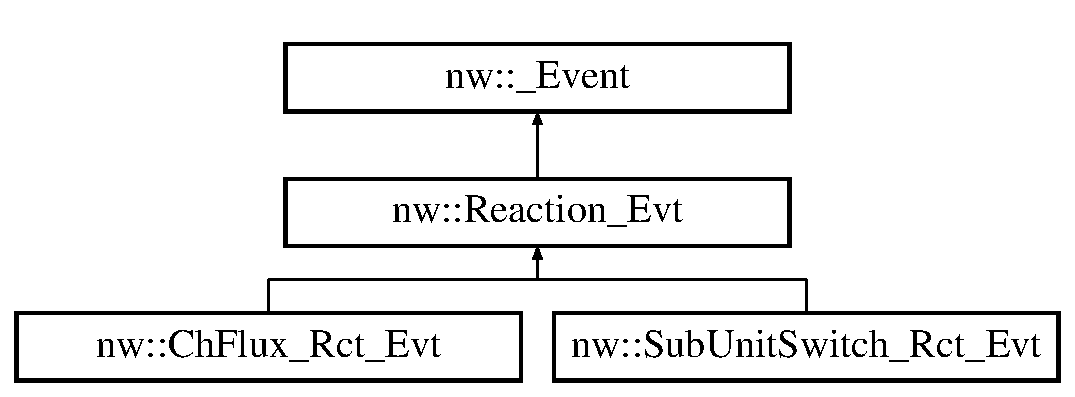
\includegraphics[height=3.000000cm]{d1/d8c/classnw_1_1_reaction___evt}
\end{center}
\end{figure}
\subsection*{Public Member Functions}
\begin{DoxyCompactItemize}
\item 
\hyperlink{classnw_1_1_reaction___evt_a582f3c60366d15e89fdd613abe4bd86d}{Reaction\+\_\+\+Evt} (long \hyperlink{classnw_1_1___event_a8f7ce287f596266dd763ec7db2f74090}{id}, string \hyperlink{classnw_1_1___event_ab4f50a54039cd4957bdca55049178562}{name}, double \hyperlink{classnw_1_1___event_afca0ae816e9834add07db8e9a6618faa}{k}, vector$<$ long $>$ \hyperlink{classnw_1_1___event_a560c8b6f9954a43f5d5f80204473b64d}{sc\+\_\+vec}, \hyperlink{namespacenw_ad7146b8b5a9de9be416847f41135722c}{Voxel\+Vector} vvc, \hyperlink{classnw_1_1_uni___rnd}{Uni\+\_\+\+Rnd} $\ast$\hyperlink{classnw_1_1___event_af92482aeea55562560573ecccd5ab108}{rg})
\begin{DoxyCompactList}\small\item\em Constructor. \end{DoxyCompactList}\item 
virtual \hyperlink{classnw_1_1_reaction___evt_a8f8ee0dfc946b6a13e2a1af9b45f6411}{$\sim$\+Reaction\+\_\+\+Evt} ()
\item 
double \hyperlink{classnw_1_1_reaction___evt_aaa2e896edd2263dbe78f5b5aa37fb091}{update} (double)
\begin{DoxyCompactList}\small\item\em Implementation of the \hyperlink{classnw_1_1___event_a882115f8652c881bc8ed43f1050ccba3}{\+\_\+\+Event\+::update()} method. \end{DoxyCompactList}\item 
void \hyperlink{classnw_1_1_reaction___evt_aec2fb342726ef17255ebf406a7c74392}{execute} ()
\begin{DoxyCompactList}\small\item\em Implementation of the \hyperlink{classnw_1_1___event_aa022418fb765582a053ac75cbc3436d6}{\+\_\+\+Event\+::execute()} method. \end{DoxyCompactList}\item 
void \hyperlink{classnw_1_1_reaction___evt_a50daf1db256ed7e0b22a29ffac76a1b6}{init} ()
\begin{DoxyCompactList}\small\item\em Implementation of the \hyperlink{classnw_1_1___event_ae2c608ee2508058d6f318ca2ca8f4317}{\+\_\+\+Event\+::init()} method. \end{DoxyCompactList}\item 
double \hyperlink{classnw_1_1_reaction___evt_a98001b8296e789db3da09791087c4a35}{get\+\_\+a} ()
\begin{DoxyCompactList}\small\item\em Implementation of the \hyperlink{classnw_1_1___event_a75945699f539cefab36eb6693a389918}{\+\_\+\+Event\+::get\+\_\+a()} method. \end{DoxyCompactList}\end{DoxyCompactItemize}
\subsection*{Protected Member Functions}
\begin{DoxyCompactItemize}
\item 
void \hyperlink{classnw_1_1_reaction___evt_acc544c7890cdb51e794d26a845c8441f}{build\+\_\+educt\+\_\+vector} ()
\begin{DoxyCompactList}\small\item\em builds the educt vector. \end{DoxyCompactList}\item 
double \hyperlink{classnw_1_1_reaction___evt_ace67f5106799204a2f2cde8c6982589b}{calc\+\_\+tau} (long)
\begin{DoxyCompactList}\small\item\em calculates a new tau value using a random number. The calc\+\_\+tau function is dependent on the reaction order\+: \end{DoxyCompactList}\end{DoxyCompactItemize}
\subsection*{Protected Attributes}
\begin{DoxyCompactItemize}
\item 
vector$<$ long $>$ \hyperlink{classnw_1_1_reaction___evt_ae20c8b7d42ef1607200e1e2541db9a70}{educt\+\_\+vec}
\begin{DoxyCompactList}\small\item\em Educt vector holds pointer to each species that is an educt of this reaction. \end{DoxyCompactList}\end{DoxyCompactItemize}


\subsection{Detailed Description}
Implementation of the reaction of one ore two molecules. 

In contrast to the Diffusion\+\_\+\+Event the Reaction\+\_\+\+Event alters the state vector of only one Voxel per simulation step. 

\subsection{Constructor \& Destructor Documentation}
\hypertarget{classnw_1_1_reaction___evt_a582f3c60366d15e89fdd613abe4bd86d}{\index{nw\+::\+Reaction\+\_\+\+Evt@{nw\+::\+Reaction\+\_\+\+Evt}!Reaction\+\_\+\+Evt@{Reaction\+\_\+\+Evt}}
\index{Reaction\+\_\+\+Evt@{Reaction\+\_\+\+Evt}!nw\+::\+Reaction\+\_\+\+Evt@{nw\+::\+Reaction\+\_\+\+Evt}}
\subsubsection[{Reaction\+\_\+\+Evt}]{\setlength{\rightskip}{0pt plus 5cm}nw\+::\+Reaction\+\_\+\+Evt\+::\+Reaction\+\_\+\+Evt (
\begin{DoxyParamCaption}
\item[{long}]{id, }
\item[{string}]{name, }
\item[{double}]{k, }
\item[{vector$<$ long $>$}]{sc\+\_\+vec, }
\item[{{\bf Voxel\+Vector}}]{vvc, }
\item[{{\bf Uni\+\_\+\+Rnd} $\ast$}]{rg}
\end{DoxyParamCaption}
)\hspace{0.3cm}{\ttfamily [inline]}}}\label{classnw_1_1_reaction___evt_a582f3c60366d15e89fdd613abe4bd86d}


Constructor. 


\begin{DoxyParams}{Parameters}
{\em id} & \hyperlink{classnw_1_1___event}{\+\_\+\+Event} I\+D \\
\hline
{\em name} & \hyperlink{classnw_1_1___event}{\+\_\+\+Event} name \\
\hline
{\em k} & \hyperlink{classnw_1_1___event}{\+\_\+\+Event} rate constant \\
\hline
{\em vvc} & \hyperlink{classnw_1_1___event}{\+\_\+\+Event} voxel vector \\
\hline
{\em sc\+\_\+vec} & state change vector of the reaction event \\
\hline
{\em rg} & \hyperlink{classnw_1_1___event}{\+\_\+\+Event} pointer to a Random\+\_\+\+Generator. \\
\hline
\end{DoxyParams}

\begin{DoxyCode}
23                                                                                                    :
24         \hyperlink{classnw_1_1___event_a5efb757db20b083de6da605ea4b2bbae}{\_Event}(\textcolor{keywordtype}{id},\hyperlink{classnw_1_1___event_ab4f50a54039cd4957bdca55049178562}{name},\hyperlink{classnw_1_1___event_afca0ae816e9834add07db8e9a6618faa}{k},vvc,\hyperlink{classnw_1_1___event_af92482aeea55562560573ecccd5ab108}{rg})\{
25         this->\hyperlink{classnw_1_1___event_a560c8b6f9954a43f5d5f80204473b64d}{sc\_vec} = \hyperlink{classnw_1_1___event_a560c8b6f9954a43f5d5f80204473b64d}{sc\_vec};
26     \}
\end{DoxyCode}
\hypertarget{classnw_1_1_reaction___evt_a8f8ee0dfc946b6a13e2a1af9b45f6411}{\index{nw\+::\+Reaction\+\_\+\+Evt@{nw\+::\+Reaction\+\_\+\+Evt}!````~Reaction\+\_\+\+Evt@{$\sim$\+Reaction\+\_\+\+Evt}}
\index{````~Reaction\+\_\+\+Evt@{$\sim$\+Reaction\+\_\+\+Evt}!nw\+::\+Reaction\+\_\+\+Evt@{nw\+::\+Reaction\+\_\+\+Evt}}
\subsubsection[{$\sim$\+Reaction\+\_\+\+Evt}]{\setlength{\rightskip}{0pt plus 5cm}virtual nw\+::\+Reaction\+\_\+\+Evt\+::$\sim$\+Reaction\+\_\+\+Evt (
\begin{DoxyParamCaption}
{}
\end{DoxyParamCaption}
)\hspace{0.3cm}{\ttfamily [inline]}, {\ttfamily [virtual]}}}\label{classnw_1_1_reaction___evt_a8f8ee0dfc946b6a13e2a1af9b45f6411}
Destructor 
\begin{DoxyCode}
28 \{\};
\end{DoxyCode}


\subsection{Member Function Documentation}
\hypertarget{classnw_1_1_reaction___evt_acc544c7890cdb51e794d26a845c8441f}{\index{nw\+::\+Reaction\+\_\+\+Evt@{nw\+::\+Reaction\+\_\+\+Evt}!build\+\_\+educt\+\_\+vector@{build\+\_\+educt\+\_\+vector}}
\index{build\+\_\+educt\+\_\+vector@{build\+\_\+educt\+\_\+vector}!nw\+::\+Reaction\+\_\+\+Evt@{nw\+::\+Reaction\+\_\+\+Evt}}
\subsubsection[{build\+\_\+educt\+\_\+vector}]{\setlength{\rightskip}{0pt plus 5cm}void nw\+::\+Reaction\+\_\+\+Evt\+::build\+\_\+educt\+\_\+vector (
\begin{DoxyParamCaption}
{}
\end{DoxyParamCaption}
)\hspace{0.3cm}{\ttfamily [protected]}}}\label{classnw_1_1_reaction___evt_acc544c7890cdb51e794d26a845c8441f}


builds the educt vector. 

The educt vector holds pointer to each species that is an educt of this reaction. It facilitates the update procedure 
\begin{DoxyCode}
98                                      \{
99     \textcolor{keywordflow}{for}(\textcolor{keywordtype}{size\_t} i = 0; i < \hyperlink{classnw_1_1___event_a560c8b6f9954a43f5d5f80204473b64d}{sc\_vec}.size(); ++i)\{
100         \textcolor{keywordflow}{if}(\hyperlink{classnw_1_1___event_a560c8b6f9954a43f5d5f80204473b64d}{sc\_vec}[i] < 0)
101             \hyperlink{classnw_1_1_reaction___evt_ae20c8b7d42ef1607200e1e2541db9a70}{educt\_vec}.push\_back(i);
102     \}
103 \}
\end{DoxyCode}
\hypertarget{classnw_1_1_reaction___evt_ace67f5106799204a2f2cde8c6982589b}{\index{nw\+::\+Reaction\+\_\+\+Evt@{nw\+::\+Reaction\+\_\+\+Evt}!calc\+\_\+tau@{calc\+\_\+tau}}
\index{calc\+\_\+tau@{calc\+\_\+tau}!nw\+::\+Reaction\+\_\+\+Evt@{nw\+::\+Reaction\+\_\+\+Evt}}
\subsubsection[{calc\+\_\+tau}]{\setlength{\rightskip}{0pt plus 5cm}double nw\+::\+Reaction\+\_\+\+Evt\+::calc\+\_\+tau (
\begin{DoxyParamCaption}
\item[{long}]{vid}
\end{DoxyParamCaption}
)\hspace{0.3cm}{\ttfamily [protected]}}}\label{classnw_1_1_reaction___evt_ace67f5106799204a2f2cde8c6982589b}


calculates a new tau value using a random number. The calc\+\_\+tau function is dependent on the reaction order\+: 


\begin{DoxyItemize}
\item 1. order\+: -\/ln(r)/a(j)(x,t) = -\/ln(r)/(educt $\ast$ c(j))
\item 2. order\+: -\/ln(r)/a(j)(x,t) = -\/ln(r)/(educt(1) $\ast$ educt (2) $\ast$ c(j)) only first and second order reactions are allowed! 
\end{DoxyItemize}
\begin{DoxyCode}
105                                      \{
106 
107 \textcolor{comment}{//  make sure the educt vector is valid -> only first -and second order reactions are allowed}
108     \textcolor{keywordflow}{if}(\hyperlink{classnw_1_1_reaction___evt_ae20c8b7d42ef1607200e1e2541db9a70}{educt\_vec}.size() > 0 && \hyperlink{classnw_1_1_reaction___evt_ae20c8b7d42ef1607200e1e2541db9a70}{educt\_vec}.size() <= 2)\{
109         \textcolor{keywordtype}{double} a = \hyperlink{classnw_1_1___event_a29c77fb164e745cdb5c5fda4f191cd37}{c};
110         \textcolor{keywordflow}{for} (\textcolor{keywordtype}{size\_t} i = 0; i < \hyperlink{classnw_1_1_reaction___evt_ae20c8b7d42ef1607200e1e2541db9a70}{educt\_vec}.size(); ++i)\{
111             a *= \hyperlink{classnw_1_1___event_a6351b58d94923ed58e0b2cf6c9445d2e}{tv\_vec}[vid].v->get\_state\_vec()->at(\hyperlink{classnw_1_1_reaction___evt_ae20c8b7d42ef1607200e1e2541db9a70}{educt\_vec}[i])->get\_n\_molecules();
112         \}
113         \hyperlink{classnw_1_1___event_a6351b58d94923ed58e0b2cf6c9445d2e}{tv\_vec}[vid].t = -log(\hyperlink{classnw_1_1___event_af92482aeea55562560573ecccd5ab108}{rg}->\hyperlink{classnw_1_1_uni___rnd_ad7883ef0ce4c591612bcb41678104773}{get\_Uni\_Rnd}()) / a;
114 
115         \textcolor{keywordflow}{return} \hyperlink{classnw_1_1___event_a6351b58d94923ed58e0b2cf6c9445d2e}{tv\_vec}[vid].t;
116     \} \textcolor{keywordflow}{else} \{
117         cout <<\textcolor{stringliteral}{"ERROR: Only first and second order reactions are allowed! Check sc\_vec of:"} << this->
      \hyperlink{classnw_1_1___event_ab4f50a54039cd4957bdca55049178562}{name} <<endl;
118         exit(0);
119     \}
120 \}
\end{DoxyCode}
\hypertarget{classnw_1_1_reaction___evt_aec2fb342726ef17255ebf406a7c74392}{\index{nw\+::\+Reaction\+\_\+\+Evt@{nw\+::\+Reaction\+\_\+\+Evt}!execute@{execute}}
\index{execute@{execute}!nw\+::\+Reaction\+\_\+\+Evt@{nw\+::\+Reaction\+\_\+\+Evt}}
\subsubsection[{execute}]{\setlength{\rightskip}{0pt plus 5cm}void nw\+::\+Reaction\+\_\+\+Evt\+::execute (
\begin{DoxyParamCaption}
{}
\end{DoxyParamCaption}
)\hspace{0.3cm}{\ttfamily [virtual]}}}\label{classnw_1_1_reaction___evt_aec2fb342726ef17255ebf406a7c74392}


Implementation of the \hyperlink{classnw_1_1___event_aa022418fb765582a053ac75cbc3436d6}{\+\_\+\+Event\+::execute()} method. 



Implements \hyperlink{classnw_1_1___event_aa022418fb765582a053ac75cbc3436d6}{nw\+::\+\_\+\+Event}.



Reimplemented in \hyperlink{classnw_1_1_sub_unit_switch___rct___evt_ab89891fae9287edc9d9a215788706093}{nw\+::\+Sub\+Unit\+Switch\+\_\+\+Rct\+\_\+\+Evt}.


\begin{DoxyCode}
28                           \{
29     \textcolor{keywordflow}{try}\{
30 \textcolor{comment}{//      execute event by using the state change vector}
31         \hyperlink{classnw_1_1___event_a6351b58d94923ed58e0b2cf6c9445d2e}{tv\_vec}[\hyperlink{classnw_1_1___event_a7864559e204c087306e3becb5b81fb26}{nextVoxel}].v->update\_state(\hyperlink{classnw_1_1___event_a560c8b6f9954a43f5d5f80204473b64d}{sc\_vec});
32 
33 \textcolor{comment}{//      set dirty flag to indicate that dependent events have to be updated}
34         this->\hyperlink{classnw_1_1___event_aaa705b35c06c0cb2e0a4f3daa9ee8037}{dirty\_flag} = \textcolor{keyword}{true};
35         \textcolor{keywordflow}{for}(\textcolor{keywordtype}{size\_t} i = 0; i < \hyperlink{classnw_1_1___event_a3f87b2dff69d07977f0a5e10936f38f6}{dep\_list}.size(); i++)\{
36             \hyperlink{classnw_1_1___event_a3f87b2dff69d07977f0a5e10936f38f6}{dep\_list}[i]->set\_flag(\textcolor{keyword}{true});
37         \}
38     \}
39     \textcolor{keywordflow}{catch}(exception& e)\{
40         cout << \textcolor{stringliteral}{"Reaction\_Evt::execute(): "} << e.what();
41     \}
42 \}
\end{DoxyCode}
\hypertarget{classnw_1_1_reaction___evt_a98001b8296e789db3da09791087c4a35}{\index{nw\+::\+Reaction\+\_\+\+Evt@{nw\+::\+Reaction\+\_\+\+Evt}!get\+\_\+a@{get\+\_\+a}}
\index{get\+\_\+a@{get\+\_\+a}!nw\+::\+Reaction\+\_\+\+Evt@{nw\+::\+Reaction\+\_\+\+Evt}}
\subsubsection[{get\+\_\+a}]{\setlength{\rightskip}{0pt plus 5cm}double nw\+::\+Reaction\+\_\+\+Evt\+::get\+\_\+a (
\begin{DoxyParamCaption}
{}
\end{DoxyParamCaption}
)\hspace{0.3cm}{\ttfamily [virtual]}}}\label{classnw_1_1_reaction___evt_a98001b8296e789db3da09791087c4a35}


Implementation of the \hyperlink{classnw_1_1___event_a75945699f539cefab36eb6693a389918}{\+\_\+\+Event\+::get\+\_\+a()} method. 

\begin{DoxyReturn}{Returns}
a0 of this \hyperlink{classnw_1_1___event}{\+\_\+\+Event} 
\end{DoxyReturn}


Implements \hyperlink{classnw_1_1___event_a75945699f539cefab36eb6693a389918}{nw\+::\+\_\+\+Event}.


\begin{DoxyCode}
86                           \{
87     \textcolor{keywordtype}{double} a\_ges = 0;
88     \textcolor{keywordflow}{for}(\textcolor{keywordtype}{size\_t} i = 0; i < \hyperlink{classnw_1_1___event_a6351b58d94923ed58e0b2cf6c9445d2e}{tv\_vec}.size(); ++i)\{
89         \textcolor{keywordtype}{double} a = \hyperlink{classnw_1_1___event_a29c77fb164e745cdb5c5fda4f191cd37}{c};
90         \textcolor{keywordflow}{for} (\textcolor{keywordtype}{size\_t} j = 0; j < \hyperlink{classnw_1_1_reaction___evt_ae20c8b7d42ef1607200e1e2541db9a70}{educt\_vec}.size(); ++j)\{
91             a *= \hyperlink{classnw_1_1___event_a6351b58d94923ed58e0b2cf6c9445d2e}{tv\_vec}[i].v->get\_state\_vec()->at(\hyperlink{classnw_1_1_reaction___evt_ae20c8b7d42ef1607200e1e2541db9a70}{educt\_vec}[j])->get\_n\_molecules();
92         \}
93         a\_ges += a;
94     \}
95     \textcolor{keywordflow}{return} a\_ges;
96 \}
\end{DoxyCode}
\hypertarget{classnw_1_1_reaction___evt_a50daf1db256ed7e0b22a29ffac76a1b6}{\index{nw\+::\+Reaction\+\_\+\+Evt@{nw\+::\+Reaction\+\_\+\+Evt}!init@{init}}
\index{init@{init}!nw\+::\+Reaction\+\_\+\+Evt@{nw\+::\+Reaction\+\_\+\+Evt}}
\subsubsection[{init}]{\setlength{\rightskip}{0pt plus 5cm}void nw\+::\+Reaction\+\_\+\+Evt\+::init (
\begin{DoxyParamCaption}
{}
\end{DoxyParamCaption}
)\hspace{0.3cm}{\ttfamily [virtual]}}}\label{classnw_1_1_reaction___evt_a50daf1db256ed7e0b22a29ffac76a1b6}


Implementation of the \hyperlink{classnw_1_1___event_ae2c608ee2508058d6f318ca2ca8f4317}{\+\_\+\+Event\+::init()} method. 



Implements \hyperlink{classnw_1_1___event_ae2c608ee2508058d6f318ca2ca8f4317}{nw\+::\+\_\+\+Event}.


\begin{DoxyCode}
12                        \{
13 
14 \textcolor{comment}{//  build educt vector}
15     \hyperlink{classnw_1_1_reaction___evt_acc544c7890cdb51e794d26a845c8441f}{build\_educt\_vector}();
16 
17 \textcolor{comment}{//  calculate the correct probability rate constant depending on the reaction order.}
18     \textcolor{keywordflow}{if} (\hyperlink{classnw_1_1_reaction___evt_ae20c8b7d42ef1607200e1e2541db9a70}{educt\_vec}.size() == 1)\{
19         this->\hyperlink{classnw_1_1___event_a29c77fb164e745cdb5c5fda4f191cd37}{c} = \hyperlink{classnw_1_1___event_afca0ae816e9834add07db8e9a6618faa}{k};
20     \}\textcolor{keywordflow}{else} \textcolor{keywordflow}{if}(\hyperlink{classnw_1_1_reaction___evt_ae20c8b7d42ef1607200e1e2541db9a70}{educt\_vec}.size() == 2)\{
21         this->\hyperlink{classnw_1_1___event_a29c77fb164e745cdb5c5fda4f191cd37}{c} = \hyperlink{classnw_1_1___event_afca0ae816e9834add07db8e9a6618faa}{k}/(\hyperlink{classnw_1_1___event_a6351b58d94923ed58e0b2cf6c9445d2e}{tv\_vec}[0].v->get\_volume()*\hyperlink{namespacenw_ad890cfa7dd9eaf8d5b6754723e516c4a}{N\_AVO}*1e-6);
22     \}
23 
24 \textcolor{comment}{//  update the Reaction Event the first time}
25     \hyperlink{classnw_1_1_reaction___evt_aaa2e896edd2263dbe78f5b5aa37fb091}{update}(0);
26 \}
\end{DoxyCode}
\hypertarget{classnw_1_1_reaction___evt_aaa2e896edd2263dbe78f5b5aa37fb091}{\index{nw\+::\+Reaction\+\_\+\+Evt@{nw\+::\+Reaction\+\_\+\+Evt}!update@{update}}
\index{update@{update}!nw\+::\+Reaction\+\_\+\+Evt@{nw\+::\+Reaction\+\_\+\+Evt}}
\subsubsection[{update}]{\setlength{\rightskip}{0pt plus 5cm}double nw\+::\+Reaction\+\_\+\+Evt\+::update (
\begin{DoxyParamCaption}
\item[{double}]{last\+\_\+tau}
\end{DoxyParamCaption}
)\hspace{0.3cm}{\ttfamily [virtual]}}}\label{classnw_1_1_reaction___evt_aaa2e896edd2263dbe78f5b5aa37fb091}


Implementation of the \hyperlink{classnw_1_1___event_a882115f8652c881bc8ed43f1050ccba3}{\+\_\+\+Event\+::update()} method. 


\begin{DoxyParams}{Parameters}
{\em last\+\_\+tau} & last tau value to update the system time. \\
\hline
\end{DoxyParams}
\begin{DoxyReturn}{Returns}
The new tau value, so system can sort it right away.
\end{DoxyReturn}
If dirty\+\_\+flag is true, this event depends on the event that fired during the previosu simulation step. For each voxel that has been modified, the \hyperlink{classnw_1_1___event}{\+\_\+\+Event} specific tau value has to be updated. All the other tau values have to be adapted to the global system time 

Implements \hyperlink{classnw_1_1___event_a882115f8652c881bc8ed43f1050ccba3}{nw\+::\+\_\+\+Event}.


\begin{DoxyCode}
44                                           \{
45 
46     \textcolor{keywordtype}{double} minTau = INFINITY;
47 
48 \textcolor{comment}{//  check if this event depends on the last executed event}
49     \textcolor{keywordflow}{if}(this->\hyperlink{classnw_1_1___event_aaa705b35c06c0cb2e0a4f3daa9ee8037}{dirty\_flag})\{
50 \textcolor{comment}{//      run through the tv vector}
51         \textcolor{keywordflow}{for} (\textcolor{keywordtype}{size\_t} i = 0; i < \hyperlink{classnw_1_1___event_a6351b58d94923ed58e0b2cf6c9445d2e}{tv\_vec}.size(); ++i)\{
52 \textcolor{comment}{//          check for voxel that have been affected by last executed event}
53             \textcolor{keywordflow}{if} (\hyperlink{classnw_1_1___event_a6351b58d94923ed58e0b2cf6c9445d2e}{tv\_vec}[i].v->get\_dirty\_flag())\{
54 \textcolor{comment}{//              find smallest tau value (->next voxel) for this event}
55                 \textcolor{keywordflow}{if}(\hyperlink{classnw_1_1_reaction___evt_ace67f5106799204a2f2cde8c6982589b}{calc\_tau}(i) < minTau)\{
56                     minTau = \hyperlink{classnw_1_1___event_a6351b58d94923ed58e0b2cf6c9445d2e}{tv\_vec}[i].t;
57                     \hyperlink{classnw_1_1___event_a7864559e204c087306e3becb5b81fb26}{nextVoxel} = i;
58                 \}
59 \textcolor{comment}{//          voxel has not been affected by last event}
60             \} \textcolor{keywordflow}{else} \{
61 \textcolor{comment}{//              adjust tau value to global times scale}
62                 \hyperlink{classnw_1_1___event_a6351b58d94923ed58e0b2cf6c9445d2e}{tv\_vec}[i].t -= last\_tau;
63 \textcolor{comment}{//              find smallest tau value (->next voxel) for this event}
64                 \textcolor{keywordflow}{if}(\hyperlink{classnw_1_1___event_a6351b58d94923ed58e0b2cf6c9445d2e}{tv\_vec}[i].t < minTau)\{
65                     minTau = \hyperlink{classnw_1_1___event_a6351b58d94923ed58e0b2cf6c9445d2e}{tv\_vec}[i].t;
66                     \hyperlink{classnw_1_1___event_a7864559e204c087306e3becb5b81fb26}{nextVoxel} = i;
67                 \}
68             \}
69         \}
70 \textcolor{comment}{//  event has not been affected by last event}
71     \} \textcolor{keywordflow}{else}  \{
72 \textcolor{comment}{//      adjust tau values to global times scale}
73         \textcolor{keywordflow}{for} (\textcolor{keywordtype}{size\_t} i = 0; i < \hyperlink{classnw_1_1___event_a6351b58d94923ed58e0b2cf6c9445d2e}{tv\_vec}.size(); ++i) \{
74             \hyperlink{classnw_1_1___event_a6351b58d94923ed58e0b2cf6c9445d2e}{tv\_vec}[i].t -= last\_tau;
75             \textcolor{keywordflow}{if}(\hyperlink{classnw_1_1___event_a6351b58d94923ed58e0b2cf6c9445d2e}{tv\_vec}[i].t < minTau)\{
76                 minTau = \hyperlink{classnw_1_1___event_a6351b58d94923ed58e0b2cf6c9445d2e}{tv\_vec}[i].t;
77                 \hyperlink{classnw_1_1___event_a7864559e204c087306e3becb5b81fb26}{nextVoxel} = i;
78             \}
79         \}
80     \}
81 
82     this->\hyperlink{classnw_1_1___event_aaa705b35c06c0cb2e0a4f3daa9ee8037}{dirty\_flag} = \textcolor{keyword}{false};
83     \textcolor{keywordflow}{return} minTau;
84 \}
\end{DoxyCode}


\subsection{Member Data Documentation}
\hypertarget{classnw_1_1_reaction___evt_ae20c8b7d42ef1607200e1e2541db9a70}{\index{nw\+::\+Reaction\+\_\+\+Evt@{nw\+::\+Reaction\+\_\+\+Evt}!educt\+\_\+vec@{educt\+\_\+vec}}
\index{educt\+\_\+vec@{educt\+\_\+vec}!nw\+::\+Reaction\+\_\+\+Evt@{nw\+::\+Reaction\+\_\+\+Evt}}
\subsubsection[{educt\+\_\+vec}]{\setlength{\rightskip}{0pt plus 5cm}vector$<$long$>$ nw\+::\+Reaction\+\_\+\+Evt\+::educt\+\_\+vec\hspace{0.3cm}{\ttfamily [protected]}}}\label{classnw_1_1_reaction___evt_ae20c8b7d42ef1607200e1e2541db9a70}


Educt vector holds pointer to each species that is an educt of this reaction. 



The documentation for this class was generated from the following files\+:\begin{DoxyCompactItemize}
\item 
Events/\hyperlink{_reaction___evt_8h}{Reaction\+\_\+\+Evt.\+h}\item 
Events/\hyperlink{_reaction___evt_8cpp}{Reaction\+\_\+\+Evt.\+cpp}\end{DoxyCompactItemize}

\hypertarget{classnw_1_1_standard___ipt}{\section{nw\+:\+:Standard\+\_\+\+Ipt Class Reference}
\label{classnw_1_1_standard___ipt}\index{nw\+::\+Standard\+\_\+\+Ipt@{nw\+::\+Standard\+\_\+\+Ipt}}
}


Input class that parses a .xml files and generates a \hyperlink{classnw_1_1_gillespie___sys}{Gillespie\+\_\+\+Sys}.  




{\ttfamily \#include $<$Standard\+\_\+\+Ipt.\+h$>$}

Inheritance diagram for nw\+:\+:Standard\+\_\+\+Ipt\+:\begin{figure}[H]
\begin{center}
\leavevmode
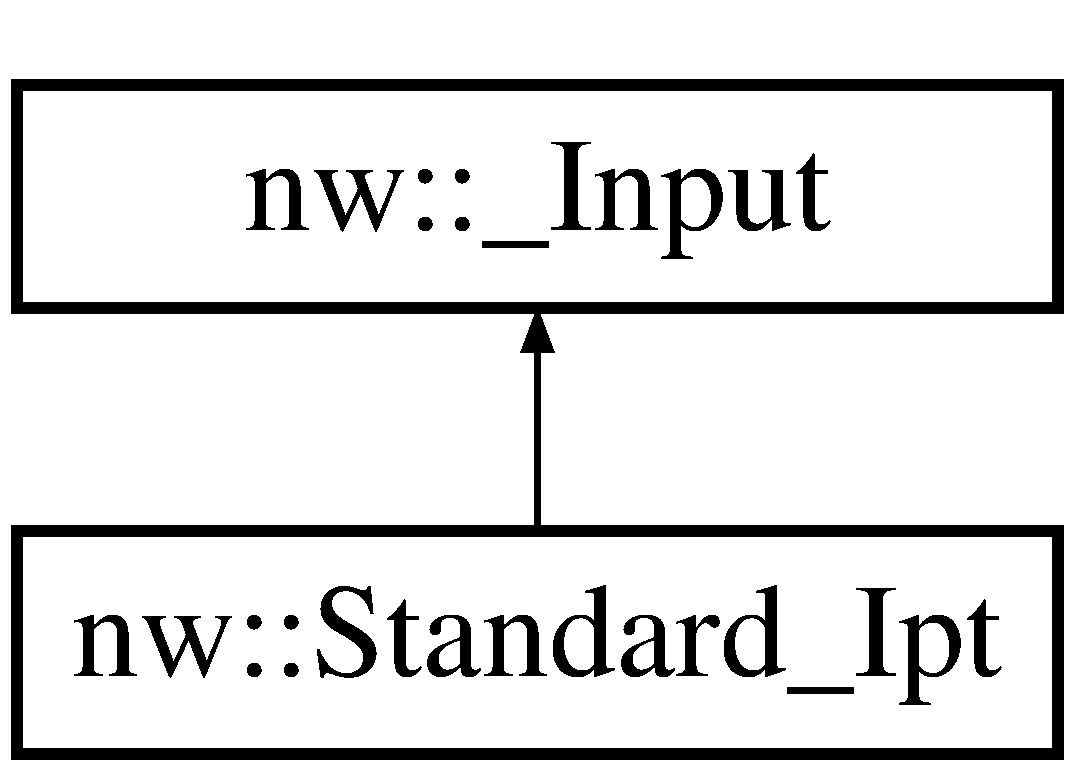
\includegraphics[height=2.000000cm]{d0/d19/classnw_1_1_standard___ipt}
\end{center}
\end{figure}
\subsection*{Classes}
\begin{DoxyCompactItemize}
\item 
struct \hyperlink{structnw_1_1_standard___ipt_1_1xml___ch___spc}{xml\+\_\+\+Ch\+\_\+\+Spc}
\begin{DoxyCompactList}\small\item\em Structure with attributes of the \hyperlink{classnw_1_1_channel___spc}{Channel\+\_\+\+Spc} class. \end{DoxyCompactList}\item 
struct \hyperlink{structnw_1_1_standard___ipt_1_1xml___ch_flux___rct___evt}{xml\+\_\+\+Ch\+Flux\+\_\+\+Rct\+\_\+\+Evt}
\begin{DoxyCompactList}\small\item\em Structure with attributes of the \hyperlink{classnw_1_1_ch_flux___rct___evt}{Ch\+Flux\+\_\+\+Rct\+\_\+\+Evt} class. \end{DoxyCompactList}\item 
struct \hyperlink{structnw_1_1_standard___ipt_1_1xml___dif___evt}{xml\+\_\+\+Dif\+\_\+\+Evt}
\begin{DoxyCompactList}\small\item\em Structure with attributes of the \hyperlink{classnw_1_1_diffusion___evt}{Diffusion\+\_\+\+Evt} class. \end{DoxyCompactList}\item 
struct \hyperlink{structnw_1_1_standard___ipt_1_1xml__evt}{xml\+\_\+evt}
\begin{DoxyCompactList}\small\item\em Structure with attributes of the \hyperlink{classnw_1_1___event}{\+\_\+\+Event} class. \end{DoxyCompactList}\item 
struct \hyperlink{structnw_1_1_standard___ipt_1_1xml__gen__data}{xml\+\_\+gen\+\_\+data}
\begin{DoxyCompactList}\small\item\em Structure with attributes representing general data necessary for a system. \end{DoxyCompactList}\item 
struct \hyperlink{structnw_1_1_standard___ipt_1_1xml___rct___evt}{xml\+\_\+\+Rct\+\_\+\+Evt}
\begin{DoxyCompactList}\small\item\em Structure with attributes of the \hyperlink{classnw_1_1_reaction___evt}{Reaction\+\_\+\+Evt} class. \end{DoxyCompactList}\item 
struct \hyperlink{structnw_1_1_standard___ipt_1_1xml__spc}{xml\+\_\+spc}
\begin{DoxyCompactList}\small\item\em Structure with attributes of the \hyperlink{classnw_1_1___species}{\+\_\+\+Species} class. \end{DoxyCompactList}\item 
struct \hyperlink{structnw_1_1_standard___ipt_1_1xml___su_switch___rct___evt}{xml\+\_\+\+Su\+Switch\+\_\+\+Rct\+\_\+\+Evt}
\begin{DoxyCompactList}\small\item\em Structure with attributes of the \hyperlink{classnw_1_1_sub_unit_switch___rct___evt}{Sub\+Unit\+Switch\+\_\+\+Rct\+\_\+\+Evt} class. \end{DoxyCompactList}\item 
struct \hyperlink{structnw_1_1_standard___ipt_1_1xml__vxl}{xml\+\_\+vxl}
\begin{DoxyCompactList}\small\item\em Structure with attributes of the \hyperlink{classnw_1_1___voxel}{\+\_\+\+Voxel} class. \end{DoxyCompactList}\end{DoxyCompactItemize}
\subsection*{Public Member Functions}
\begin{DoxyCompactItemize}
\item 
\hyperlink{classnw_1_1_standard___ipt_a94434a8c2de8304a6ab626cdc11ea442}{Standard\+\_\+\+Ipt} (string input\+\_\+path, string \hyperlink{classnw_1_1_standard___ipt_a22ca09b593a0438676fd560f168e76f9}{output\+\_\+dir\+\_\+path})
\begin{DoxyCompactList}\small\item\em Constructor. \end{DoxyCompactList}\item 
\hyperlink{classnw_1_1_standard___ipt_a7d66e39904aa2462474703672b790caf}{$\sim$\+Standard\+\_\+\+Ipt} ()
\begin{DoxyCompactList}\small\item\em Destructor. \end{DoxyCompactList}\item 
\hyperlink{classnw_1_1___system}{\+\_\+\+System} $\ast$ \hyperlink{classnw_1_1_standard___ipt_ae5ae0e8b67291839d71df934bfc17238}{get\+\_\+\+System} ()
\begin{DoxyCompactList}\small\item\em Implementation of the \hyperlink{classnw_1_1___input_a5bb57fdb6dfcf4efa7b64e096594a8b3}{\+\_\+\+Input\+::get\+\_\+\+System()} method. \end{DoxyCompactList}\end{DoxyCompactItemize}
\subsection*{Private Member Functions}
\begin{DoxyCompactItemize}
\item 
void \hyperlink{classnw_1_1_standard___ipt_a0e29f3f6a4a01caa99d5ca151748be2c}{read\+\_\+\+Sim\+\_\+\+Data} ()
\begin{DoxyCompactList}\small\item\em Extract general simulation data and store it in the xgd struct. \end{DoxyCompactList}\item 
void \hyperlink{classnw_1_1_standard___ipt_ad23a7e58b69db65c74a9168fde457b19}{read\+\_\+\+Events} (pugi\+::xml\+\_\+node const \&nod)
\begin{DoxyCompactList}\small\item\em Read events from parse result. \end{DoxyCompactList}\item 
void \hyperlink{classnw_1_1_standard___ipt_a6024eab893f556075f463a685f2f28eb}{read\+\_\+\+Voxel} (pugi\+::xml\+\_\+node const \&nod)
\begin{DoxyCompactList}\small\item\em Read voxels from parse result. \end{DoxyCompactList}\item 
void \hyperlink{classnw_1_1_standard___ipt_a488e5aad95f3d66c6bfbb5f3e5daed3c}{read\+\_\+\+Species} (pugi\+::xml\+\_\+node const \&nod)
\begin{DoxyCompactList}\small\item\em Read species from parse result. \end{DoxyCompactList}\item 
void \hyperlink{classnw_1_1_standard___ipt_af38174edfc9d7be8bd9ee2c8bc6c4181}{alloc\+\_\+\+Events} ()
\begin{DoxyCompactList}\small\item\em Create \hyperlink{classnw_1_1___event}{\+\_\+\+Event} objects. \end{DoxyCompactList}\item 
void \hyperlink{classnw_1_1_standard___ipt_a0f07caf506c0610596e8b296955ac47a}{alloc\+\_\+\+Voxel} ()
\begin{DoxyCompactList}\small\item\em Create \hyperlink{classnw_1_1___voxel}{\+\_\+\+Voxel} objects. \end{DoxyCompactList}\item 
void \hyperlink{classnw_1_1_standard___ipt_ac234f7433af26ad614e3f43088f13e48}{alloc\+\_\+\+Species} ()
\begin{DoxyCompactList}\small\item\em Create \hyperlink{classnw_1_1___species}{\+\_\+\+Species} objects. \end{DoxyCompactList}\item 
vector$<$ \hyperlink{classnw_1_1___voxel}{\+\_\+\+Voxel} $\ast$ $>$ \hyperlink{classnw_1_1_standard___ipt_a834bc59d1c945553aad59de7b23e019f}{build\+\_\+vxl\+\_\+vec} (\hyperlink{structnw_1_1_standard___ipt_1_1xml__evt}{xml\+\_\+evt} $\ast$const \&evt)
\begin{DoxyCompactList}\small\item\em Build \hyperlink{classnw_1_1___voxel}{\+\_\+\+Voxel} vector for \hyperlink{classnw_1_1___event}{\+\_\+\+Event} objects. \end{DoxyCompactList}\item 
vector$<$ long $>$ \hyperlink{classnw_1_1_standard___ipt_a5623430707739fdabf4d99599e6444a2}{build\+\_\+sc\+\_\+vector} (\hyperlink{structnw_1_1_standard___ipt_1_1xml___rct___evt}{xml\+\_\+\+Rct\+\_\+\+Evt} $\ast$const \&cxe)
\begin{DoxyCompactList}\small\item\em Build state change vector for \hyperlink{classnw_1_1_reaction___evt}{Reaction\+\_\+\+Evt} objects @ param cxe \hyperlink{structnw_1_1_standard___ipt_1_1xml___rct___evt}{xml\+\_\+\+Rct\+\_\+\+Evt} @ return \hyperlink{classnw_1_1_reaction___evt}{Reaction\+\_\+\+Evt} specific state change vector. \end{DoxyCompactList}\item 
vector$<$ \hyperlink{classnw_1_1___species}{\+\_\+\+Species} $\ast$ $>$ \hyperlink{classnw_1_1_standard___ipt_ae75407ca95fe5c6e0e2b48a892c0dcdb}{clone\+\_\+svc} ()
\begin{DoxyCompactList}\small\item\em Clone \hyperlink{classnw_1_1___species}{\+\_\+\+Species} vector. \end{DoxyCompactList}\item 
string \hyperlink{classnw_1_1_standard___ipt_a94a28b548fd1ae6dca50c8fb88d690bb}{build\+\_\+header} ()
\begin{DoxyCompactList}\small\item\em Builds console output header. \end{DoxyCompactList}\end{DoxyCompactItemize}
\subsection*{Private Attributes}
\begin{DoxyCompactItemize}
\item 
string \hyperlink{classnw_1_1_standard___ipt_a22ca09b593a0438676fd560f168e76f9}{output\+\_\+dir\+\_\+path}
\begin{DoxyCompactList}\small\item\em Output directory path. \end{DoxyCompactList}\item 
\hyperlink{structnw_1_1_standard___ipt_1_1xml__gen__data}{xml\+\_\+gen\+\_\+data} \hyperlink{classnw_1_1_standard___ipt_aad5708d9729b7a5f660dade1927b4d4e}{xgd}
\begin{DoxyCompactList}\small\item\em Structure holding general simulation data. \end{DoxyCompactList}\item 
pugi\+::xml\+\_\+document \hyperlink{classnw_1_1_standard___ipt_a08140c2c24ab36240c45d241352fc57d}{doc}
\begin{DoxyCompactList}\small\item\em D\+O\+M tree root (pugixml) \end{DoxyCompactList}\item 
char $\ast$ \hyperlink{classnw_1_1_standard___ipt_af30a47d8999101d9f83964b5be9f86a5}{p}
\item 
ofstream \hyperlink{classnw_1_1_standard___ipt_a7b8147e8b90f4adabb30e1b3fd8c40b8}{info\+\_\+path}
\begin{DoxyCompactList}\small\item\em Off-\/stream for sim\+\_\+info file that summarizes parsed xml data. \end{DoxyCompactList}\item 
\hyperlink{classnw_1_1_uni___rnd}{Uni\+\_\+\+Rnd} $\ast$ \hyperlink{classnw_1_1_standard___ipt_a18f5e3cad0d5eef81443dfaf8949ba4b}{rg}
\begin{DoxyCompactList}\small\item\em Uniform random number generator. \end{DoxyCompactList}\item 
vector$<$ \hyperlink{classnw_1_1___event}{\+\_\+\+Event} $\ast$ $>$ \hyperlink{classnw_1_1_standard___ipt_aed79f0ae61a44f1d3aceb6839a8a7733}{evc}
\begin{DoxyCompactList}\small\item\em \hyperlink{classnw_1_1___event}{\+\_\+\+Event} vector \end{DoxyCompactList}\item 
vector$<$ \hyperlink{classnw_1_1___voxel}{\+\_\+\+Voxel} $\ast$ $>$ \hyperlink{classnw_1_1_standard___ipt_a7f93dd90e12eb3a5b023e64feca48572}{vvc}
\begin{DoxyCompactList}\small\item\em \hyperlink{classnw_1_1___voxel}{\+\_\+\+Voxel} vector \end{DoxyCompactList}\item 
vector$<$ \hyperlink{classnw_1_1___species}{\+\_\+\+Species} $\ast$ $>$ \hyperlink{classnw_1_1_standard___ipt_a26fbf039d1232349799194d289febb8d}{svc}
\begin{DoxyCompactList}\small\item\em \+\_\+\+Specied vector \end{DoxyCompactList}\end{DoxyCompactItemize}
\subsection*{Additional Inherited Members}


\subsection{Detailed Description}
Input class that parses a .xml files and generates a \hyperlink{classnw_1_1_gillespie___sys}{Gillespie\+\_\+\+Sys}. 

The structure of the input .xml file represents the objects that need to be created to set up a model. The open source xml parser {\itshape pugixml} (\href{http://pugixml.org/}{\tt http\+://pugixml.\+org/}) version 0.\+9 is used. The input procedure is subdivided into three steps\+:
\begin{DoxyEnumerate}
\item .xml data is parsed with {\itshape pugixml}.
\item Parse result is analyzed and model data temporarily stored in structures.
\item Objects are created using attributes of respective structures as parameters. 
\end{DoxyEnumerate}

\subsection{Constructor \& Destructor Documentation}
\hypertarget{classnw_1_1_standard___ipt_a94434a8c2de8304a6ab626cdc11ea442}{\index{nw\+::\+Standard\+\_\+\+Ipt@{nw\+::\+Standard\+\_\+\+Ipt}!Standard\+\_\+\+Ipt@{Standard\+\_\+\+Ipt}}
\index{Standard\+\_\+\+Ipt@{Standard\+\_\+\+Ipt}!nw\+::\+Standard\+\_\+\+Ipt@{nw\+::\+Standard\+\_\+\+Ipt}}
\subsubsection[{Standard\+\_\+\+Ipt}]{\setlength{\rightskip}{0pt plus 5cm}nw\+::\+Standard\+\_\+\+Ipt\+::\+Standard\+\_\+\+Ipt (
\begin{DoxyParamCaption}
\item[{string}]{input\+\_\+path, }
\item[{string}]{output\+\_\+dir\+\_\+path}
\end{DoxyParamCaption}
)\hspace{0.3cm}{\ttfamily [inline]}}}\label{classnw_1_1_standard___ipt_a94434a8c2de8304a6ab626cdc11ea442}


Constructor. 


\begin{DoxyParams}{Parameters}
{\em input\+\_\+path} & Path to input file (.xml) \\
\hline
{\em output\+\_\+dir\+\_\+path} & Path to output directory \\
\hline
\end{DoxyParams}

\begin{DoxyCode}
31                                                            \{
32         this->\hyperlink{classnw_1_1_standard___ipt_af30a47d8999101d9f83964b5be9f86a5}{p} = (\textcolor{keywordtype}{char}*)input\_path.c\_str();
33         xml\_parse\_result result = \hyperlink{classnw_1_1_standard___ipt_a08140c2c24ab36240c45d241352fc57d}{doc}.load\_file(\hyperlink{classnw_1_1_standard___ipt_af30a47d8999101d9f83964b5be9f86a5}{p}); \textcolor{comment}{// load xml file}
34         this->\hyperlink{classnw_1_1_standard___ipt_a22ca09b593a0438676fd560f168e76f9}{output\_dir\_path} = \hyperlink{classnw_1_1_standard___ipt_a22ca09b593a0438676fd560f168e76f9}{output\_dir\_path};
35         \hyperlink{classnw_1_1_standard___ipt_a18f5e3cad0d5eef81443dfaf8949ba4b}{rg} = \textcolor{keyword}{new} Uni\_Rnd();
36     \}
\end{DoxyCode}
\hypertarget{classnw_1_1_standard___ipt_a7d66e39904aa2462474703672b790caf}{\index{nw\+::\+Standard\+\_\+\+Ipt@{nw\+::\+Standard\+\_\+\+Ipt}!````~Standard\+\_\+\+Ipt@{$\sim$\+Standard\+\_\+\+Ipt}}
\index{````~Standard\+\_\+\+Ipt@{$\sim$\+Standard\+\_\+\+Ipt}!nw\+::\+Standard\+\_\+\+Ipt@{nw\+::\+Standard\+\_\+\+Ipt}}
\subsubsection[{$\sim$\+Standard\+\_\+\+Ipt}]{\setlength{\rightskip}{0pt plus 5cm}nw\+::\+Standard\+\_\+\+Ipt\+::$\sim$\+Standard\+\_\+\+Ipt (
\begin{DoxyParamCaption}
{}
\end{DoxyParamCaption}
)}}\label{classnw_1_1_standard___ipt_a7d66e39904aa2462474703672b790caf}


Destructor. 


\begin{DoxyCode}
10                            \{
11     \textcolor{keywordflow}{if}(\hyperlink{classnw_1_1_standard___ipt_a18f5e3cad0d5eef81443dfaf8949ba4b}{rg})\{\textcolor{keyword}{delete} \hyperlink{classnw_1_1_standard___ipt_a18f5e3cad0d5eef81443dfaf8949ba4b}{rg};\hyperlink{classnw_1_1_standard___ipt_a18f5e3cad0d5eef81443dfaf8949ba4b}{rg}=NULL;\}
12     \textcolor{keywordflow}{for} (\textcolor{keywordtype}{size\_t} i=0;i<\hyperlink{classnw_1_1_standard___ipt_aad5708d9729b7a5f660dade1927b4d4e}{xgd}.\hyperlink{structnw_1_1_standard___ipt_1_1xml__gen__data_a70786e61ea513972d7c50982e101726c}{xml\_spc\_list}.size();++i)\{
13         \textcolor{keywordflow}{if}(\hyperlink{classnw_1_1_standard___ipt_aad5708d9729b7a5f660dade1927b4d4e}{xgd}.\hyperlink{structnw_1_1_standard___ipt_1_1xml__gen__data_a70786e61ea513972d7c50982e101726c}{xml\_spc\_list}[i])\{\textcolor{keyword}{delete} \hyperlink{classnw_1_1_standard___ipt_aad5708d9729b7a5f660dade1927b4d4e}{xgd}.\hyperlink{structnw_1_1_standard___ipt_1_1xml__gen__data_a70786e61ea513972d7c50982e101726c}{xml\_spc\_list}[i];
      \hyperlink{classnw_1_1_standard___ipt_aad5708d9729b7a5f660dade1927b4d4e}{xgd}.\hyperlink{structnw_1_1_standard___ipt_1_1xml__gen__data_a70786e61ea513972d7c50982e101726c}{xml\_spc\_list}[i]=NULL;\}\}
14     \textcolor{keywordflow}{for} (\textcolor{keywordtype}{size\_t} i=0;i<\hyperlink{classnw_1_1_standard___ipt_aad5708d9729b7a5f660dade1927b4d4e}{xgd}.\hyperlink{structnw_1_1_standard___ipt_1_1xml__gen__data_ab46c43b495fd3d278ffeabe88261d36e}{xml\_ch\_spc\_list}.size();++i)\{
15         \textcolor{keywordflow}{if}(\hyperlink{classnw_1_1_standard___ipt_aad5708d9729b7a5f660dade1927b4d4e}{xgd}.\hyperlink{structnw_1_1_standard___ipt_1_1xml__gen__data_ab46c43b495fd3d278ffeabe88261d36e}{xml\_ch\_spc\_list}[i])\{\textcolor{keyword}{delete} \hyperlink{classnw_1_1_standard___ipt_aad5708d9729b7a5f660dade1927b4d4e}{xgd}.
      \hyperlink{structnw_1_1_standard___ipt_1_1xml__gen__data_ab46c43b495fd3d278ffeabe88261d36e}{xml\_ch\_spc\_list}[i];\hyperlink{classnw_1_1_standard___ipt_aad5708d9729b7a5f660dade1927b4d4e}{xgd}.\hyperlink{structnw_1_1_standard___ipt_1_1xml__gen__data_ab46c43b495fd3d278ffeabe88261d36e}{xml\_ch\_spc\_list}[i]=NULL;\}\}
16     \textcolor{keywordflow}{for} (\textcolor{keywordtype}{size\_t} i=0;i<\hyperlink{classnw_1_1_standard___ipt_aad5708d9729b7a5f660dade1927b4d4e}{xgd}.\hyperlink{structnw_1_1_standard___ipt_1_1xml__gen__data_af091596661fc87ef8c7f28317555c6af}{xml\_vxl\_list}.size();++i)\{\textcolor{keywordflow}{if}(\hyperlink{classnw_1_1_standard___ipt_aad5708d9729b7a5f660dade1927b4d4e}{xgd}.
      \hyperlink{structnw_1_1_standard___ipt_1_1xml__gen__data_af091596661fc87ef8c7f28317555c6af}{xml\_vxl\_list}[i])\{
17         \textcolor{keyword}{delete} \hyperlink{classnw_1_1_standard___ipt_aad5708d9729b7a5f660dade1927b4d4e}{xgd}.\hyperlink{structnw_1_1_standard___ipt_1_1xml__gen__data_af091596661fc87ef8c7f28317555c6af}{xml\_vxl\_list}[i];\hyperlink{classnw_1_1_standard___ipt_aad5708d9729b7a5f660dade1927b4d4e}{xgd}.\hyperlink{structnw_1_1_standard___ipt_1_1xml__gen__data_af091596661fc87ef8c7f28317555c6af}{xml\_vxl\_list}[i]=NULL;\}\}
18     \textcolor{keywordflow}{for} (\textcolor{keywordtype}{size\_t} i=0;i<\hyperlink{classnw_1_1_standard___ipt_aad5708d9729b7a5f660dade1927b4d4e}{xgd}.\hyperlink{structnw_1_1_standard___ipt_1_1xml__gen__data_abc4e7ae5a154343c1d3d25917bd58a5f}{xml\_rct\_evt\_list}.size();++i)\{
19         \textcolor{keywordflow}{if}(\hyperlink{classnw_1_1_standard___ipt_aad5708d9729b7a5f660dade1927b4d4e}{xgd}.\hyperlink{structnw_1_1_standard___ipt_1_1xml__gen__data_abc4e7ae5a154343c1d3d25917bd58a5f}{xml\_rct\_evt\_list}[i])\{\textcolor{keyword}{delete} \hyperlink{classnw_1_1_standard___ipt_aad5708d9729b7a5f660dade1927b4d4e}{xgd}.
      \hyperlink{structnw_1_1_standard___ipt_1_1xml__gen__data_abc4e7ae5a154343c1d3d25917bd58a5f}{xml\_rct\_evt\_list}[i];\hyperlink{classnw_1_1_standard___ipt_aad5708d9729b7a5f660dade1927b4d4e}{xgd}.\hyperlink{structnw_1_1_standard___ipt_1_1xml__gen__data_abc4e7ae5a154343c1d3d25917bd58a5f}{xml\_rct\_evt\_list}[i]=NULL;\}\}
20     \textcolor{keywordflow}{for} (\textcolor{keywordtype}{size\_t} i=0;i<\hyperlink{classnw_1_1_standard___ipt_aad5708d9729b7a5f660dade1927b4d4e}{xgd}.\hyperlink{structnw_1_1_standard___ipt_1_1xml__gen__data_a4da34a5918c4e045ed5021da6fdbc6bf}{xml\_suSwitch\_rct\_evt\_list}.size();++i)\{
21         \textcolor{keywordflow}{if}(\hyperlink{classnw_1_1_standard___ipt_aad5708d9729b7a5f660dade1927b4d4e}{xgd}.\hyperlink{structnw_1_1_standard___ipt_1_1xml__gen__data_a4da34a5918c4e045ed5021da6fdbc6bf}{xml\_suSwitch\_rct\_evt\_list}[i])\{\textcolor{keyword}{delete} 
      \hyperlink{classnw_1_1_standard___ipt_aad5708d9729b7a5f660dade1927b4d4e}{xgd}.\hyperlink{structnw_1_1_standard___ipt_1_1xml__gen__data_a4da34a5918c4e045ed5021da6fdbc6bf}{xml\_suSwitch\_rct\_evt\_list}[i];
22         \hyperlink{classnw_1_1_standard___ipt_aad5708d9729b7a5f660dade1927b4d4e}{xgd}.\hyperlink{structnw_1_1_standard___ipt_1_1xml__gen__data_a4da34a5918c4e045ed5021da6fdbc6bf}{xml\_suSwitch\_rct\_evt\_list}[i]=NULL;\}\}
23     \textcolor{keywordflow}{for} (\textcolor{keywordtype}{size\_t} i=0;i<\hyperlink{classnw_1_1_standard___ipt_aad5708d9729b7a5f660dade1927b4d4e}{xgd}.\hyperlink{structnw_1_1_standard___ipt_1_1xml__gen__data_ae0479559e90fe38932ac604852a1541f}{xml\_chFlux\_rct\_evt\_list}.size();++i)\{
24         \textcolor{keywordflow}{if}(\hyperlink{classnw_1_1_standard___ipt_aad5708d9729b7a5f660dade1927b4d4e}{xgd}.\hyperlink{structnw_1_1_standard___ipt_1_1xml__gen__data_ae0479559e90fe38932ac604852a1541f}{xml\_chFlux\_rct\_evt\_list}[i])\{\textcolor{keyword}{delete} \hyperlink{classnw_1_1_standard___ipt_aad5708d9729b7a5f660dade1927b4d4e}{xgd}.
      \hyperlink{structnw_1_1_standard___ipt_1_1xml__gen__data_ae0479559e90fe38932ac604852a1541f}{xml\_chFlux\_rct\_evt\_list}[i];
25         \hyperlink{classnw_1_1_standard___ipt_aad5708d9729b7a5f660dade1927b4d4e}{xgd}.\hyperlink{structnw_1_1_standard___ipt_1_1xml__gen__data_ae0479559e90fe38932ac604852a1541f}{xml\_chFlux\_rct\_evt\_list}[i]=NULL;\}\}
26     \textcolor{keywordflow}{for} (\textcolor{keywordtype}{size\_t} i=0;i<\hyperlink{classnw_1_1_standard___ipt_aad5708d9729b7a5f660dade1927b4d4e}{xgd}.\hyperlink{structnw_1_1_standard___ipt_1_1xml__gen__data_a115f67778a3d29d716303c194354d2f7}{xml\_dif\_evt\_list}.size();++i)\{\textcolor{keywordflow}{if}(\hyperlink{classnw_1_1_standard___ipt_aad5708d9729b7a5f660dade1927b4d4e}{xgd}.
      \hyperlink{structnw_1_1_standard___ipt_1_1xml__gen__data_a115f67778a3d29d716303c194354d2f7}{xml\_dif\_evt\_list}[i])\{
27         \textcolor{keyword}{delete} \hyperlink{classnw_1_1_standard___ipt_aad5708d9729b7a5f660dade1927b4d4e}{xgd}.\hyperlink{structnw_1_1_standard___ipt_1_1xml__gen__data_a115f67778a3d29d716303c194354d2f7}{xml\_dif\_evt\_list}[i];\hyperlink{classnw_1_1_standard___ipt_aad5708d9729b7a5f660dade1927b4d4e}{xgd}.
      \hyperlink{structnw_1_1_standard___ipt_1_1xml__gen__data_a115f67778a3d29d716303c194354d2f7}{xml\_dif\_evt\_list}[i]=NULL;\}\}
28     \textcolor{keywordflow}{for} (\textcolor{keywordtype}{size\_t} i=0;i<\hyperlink{classnw_1_1_standard___ipt_a26fbf039d1232349799194d289febb8d}{svc}.size();++i)\{\textcolor{keywordflow}{if}(\hyperlink{classnw_1_1_standard___ipt_a26fbf039d1232349799194d289febb8d}{svc}[i])\{\textcolor{keyword}{delete} \hyperlink{classnw_1_1_standard___ipt_a26fbf039d1232349799194d289febb8d}{svc}[i];\hyperlink{classnw_1_1_standard___ipt_a26fbf039d1232349799194d289febb8d}{svc}[i]=NULL;\}\}
29     \textcolor{keywordflow}{for} (\textcolor{keywordtype}{size\_t} i=0;i<\hyperlink{classnw_1_1_standard___ipt_a7f93dd90e12eb3a5b023e64feca48572}{vvc}.size();++i)\{\textcolor{keywordflow}{if}(\hyperlink{classnw_1_1_standard___ipt_a7f93dd90e12eb3a5b023e64feca48572}{vvc}[i])\{\textcolor{keyword}{delete} \hyperlink{classnw_1_1_standard___ipt_a7f93dd90e12eb3a5b023e64feca48572}{vvc}[i];\hyperlink{classnw_1_1_standard___ipt_a7f93dd90e12eb3a5b023e64feca48572}{vvc}[i]=NULL;\}\}
30     \textcolor{keywordflow}{for} (\textcolor{keywordtype}{size\_t} i=0;i<\hyperlink{classnw_1_1_standard___ipt_aed79f0ae61a44f1d3aceb6839a8a7733}{evc}.size();++i)\{\textcolor{keywordflow}{if}(\hyperlink{classnw_1_1_standard___ipt_aed79f0ae61a44f1d3aceb6839a8a7733}{evc}[i])\{\textcolor{keyword}{delete} \hyperlink{classnw_1_1_standard___ipt_aed79f0ae61a44f1d3aceb6839a8a7733}{evc}[i];\hyperlink{classnw_1_1_standard___ipt_aed79f0ae61a44f1d3aceb6839a8a7733}{evc}[i]=NULL;\}\}
31     \textcolor{keywordflow}{if}(\hyperlink{classnw_1_1___input_af4d5765ede8af8d7f981ef179683f7e5}{s})\{\textcolor{keyword}{delete} \hyperlink{classnw_1_1___input_af4d5765ede8af8d7f981ef179683f7e5}{s};\hyperlink{classnw_1_1___input_af4d5765ede8af8d7f981ef179683f7e5}{s}=NULL;\}
32 \}
\end{DoxyCode}


\subsection{Member Function Documentation}
\hypertarget{classnw_1_1_standard___ipt_af38174edfc9d7be8bd9ee2c8bc6c4181}{\index{nw\+::\+Standard\+\_\+\+Ipt@{nw\+::\+Standard\+\_\+\+Ipt}!alloc\+\_\+\+Events@{alloc\+\_\+\+Events}}
\index{alloc\+\_\+\+Events@{alloc\+\_\+\+Events}!nw\+::\+Standard\+\_\+\+Ipt@{nw\+::\+Standard\+\_\+\+Ipt}}
\subsubsection[{alloc\+\_\+\+Events}]{\setlength{\rightskip}{0pt plus 5cm}void nw\+::\+Standard\+\_\+\+Ipt\+::alloc\+\_\+\+Events (
\begin{DoxyParamCaption}
{}
\end{DoxyParamCaption}
)\hspace{0.3cm}{\ttfamily [private]}}}\label{classnw_1_1_standard___ipt_af38174edfc9d7be8bd9ee2c8bc6c4181}


Create \hyperlink{classnw_1_1___event}{\+\_\+\+Event} objects. 


\begin{DoxyCode}
360                                \{
361     cout << \textcolor{stringliteral}{"alloc Events... "};
362 
363 \textcolor{comment}{//  create Reaction Event Voxel Vector}
364     vector<\_Voxel*> re\_vvc = \hyperlink{classnw_1_1_standard___ipt_a7f93dd90e12eb3a5b023e64feca48572}{vvc};    \textcolor{comment}{// reaction event voxel vector}
365     re\_vvc.pop\_back();              \textcolor{comment}{// doesn't contain the border voxel!}
366 
367 \textcolor{comment}{//  add all Reaction Events to the Event vector}
368     \textcolor{keywordflow}{for} (\textcolor{keywordtype}{long} i = 0; i < (long)\hyperlink{classnw_1_1_standard___ipt_aad5708d9729b7a5f660dade1927b4d4e}{xgd}.\hyperlink{structnw_1_1_standard___ipt_1_1xml__gen__data_abc4e7ae5a154343c1d3d25917bd58a5f}{xml\_rct\_evt\_list}.size(); i++)\{
369         xml\_Rct\_Evt* cxe = \hyperlink{classnw_1_1_standard___ipt_aad5708d9729b7a5f660dade1927b4d4e}{xgd}.\hyperlink{structnw_1_1_standard___ipt_1_1xml__gen__data_abc4e7ae5a154343c1d3d25917bd58a5f}{xml\_rct\_evt\_list}[i];
370         \_Event* tre =   \textcolor{keyword}{new} Reaction\_Evt(cxe->xml\_id, cxe->xml\_name, cxe->xml\_k,
371                         \hyperlink{classnw_1_1_standard___ipt_a5623430707739fdabf4d99599e6444a2}{build\_sc\_vector}(cxe), \hyperlink{classnw_1_1_standard___ipt_a834bc59d1c945553aad59de7b23e019f}{build\_vxl\_vec}(cxe), 
      \hyperlink{classnw_1_1_standard___ipt_a18f5e3cad0d5eef81443dfaf8949ba4b}{rg});
372         \hyperlink{classnw_1_1_standard___ipt_aed79f0ae61a44f1d3aceb6839a8a7733}{evc}.push\_back(tre);
373     \}
374 
375 \textcolor{comment}{//  add all Subunit Switch Reaction Events to the Event vector}
376     \textcolor{keywordflow}{for} (\textcolor{keywordtype}{long} i = 0; i < (long)\hyperlink{classnw_1_1_standard___ipt_aad5708d9729b7a5f660dade1927b4d4e}{xgd}.\hyperlink{structnw_1_1_standard___ipt_1_1xml__gen__data_a4da34a5918c4e045ed5021da6fdbc6bf}{xml\_suSwitch\_rct\_evt\_list}.size(); i++)\{
377         xml\_SuSwitch\_Rct\_Evt* cxe = \hyperlink{classnw_1_1_standard___ipt_aad5708d9729b7a5f660dade1927b4d4e}{xgd}.\hyperlink{structnw_1_1_standard___ipt_1_1xml__gen__data_a4da34a5918c4e045ed5021da6fdbc6bf}{xml\_suSwitch\_rct\_evt\_list}[i];
378         \_Event* tsusre =    \textcolor{keyword}{new} SubUnitSwitch\_Rct\_Evt(cxe->xml\_id, cxe->xml\_name, cxe->xml\_k,
379                             \hyperlink{classnw_1_1_standard___ipt_a5623430707739fdabf4d99599e6444a2}{build\_sc\_vector}(cxe), cxe->xml\_actSu\_id, cxe->xml\_channel\_id,
380                             \hyperlink{classnw_1_1_standard___ipt_a834bc59d1c945553aad59de7b23e019f}{build\_vxl\_vec}(cxe), \hyperlink{classnw_1_1_standard___ipt_a18f5e3cad0d5eef81443dfaf8949ba4b}{rg});
381         \hyperlink{classnw_1_1_standard___ipt_aed79f0ae61a44f1d3aceb6839a8a7733}{evc}.push\_back(tsusre);
382     \}
383 
384 \textcolor{comment}{//  add all Channel Flux Reaction Events to the Event vector}
385     \textcolor{keywordflow}{for} (\textcolor{keywordtype}{long} i = 0; i < (long)\hyperlink{classnw_1_1_standard___ipt_aad5708d9729b7a5f660dade1927b4d4e}{xgd}.\hyperlink{structnw_1_1_standard___ipt_1_1xml__gen__data_ae0479559e90fe38932ac604852a1541f}{xml\_chFlux\_rct\_evt\_list}.size(); i++)\{
386         xml\_ChFlux\_Rct\_Evt* cxe = \hyperlink{classnw_1_1_standard___ipt_aad5708d9729b7a5f660dade1927b4d4e}{xgd}.\hyperlink{structnw_1_1_standard___ipt_1_1xml__gen__data_ae0479559e90fe38932ac604852a1541f}{xml\_chFlux\_rct\_evt\_list}[i];
387         \_Event* tcre =  \textcolor{keyword}{new} ChFlux\_Rct\_Evt(cxe->xml\_id, cxe->xml\_name, cxe->xml\_k,
388                         \hyperlink{classnw_1_1_standard___ipt_a5623430707739fdabf4d99599e6444a2}{build\_sc\_vector}(cxe), cxe->xml\_channel\_id, 
      \hyperlink{classnw_1_1_standard___ipt_a834bc59d1c945553aad59de7b23e019f}{build\_vxl\_vec}(cxe), \hyperlink{classnw_1_1_standard___ipt_a18f5e3cad0d5eef81443dfaf8949ba4b}{rg});
389         \hyperlink{classnw_1_1_standard___ipt_aed79f0ae61a44f1d3aceb6839a8a7733}{evc}.push\_back(tcre);
390     \}
391 
392 \textcolor{comment}{//  add all Diffusion Events to the Event vector}
393     \textcolor{keywordflow}{for} (\textcolor{keywordtype}{long} i = 0; i < (long)\hyperlink{classnw_1_1_standard___ipt_aad5708d9729b7a5f660dade1927b4d4e}{xgd}.\hyperlink{structnw_1_1_standard___ipt_1_1xml__gen__data_a115f67778a3d29d716303c194354d2f7}{xml\_dif\_evt\_list}.size(); i++)\{
394         xml\_Dif\_Evt* cxe = \hyperlink{classnw_1_1_standard___ipt_aad5708d9729b7a5f660dade1927b4d4e}{xgd}.\hyperlink{structnw_1_1_standard___ipt_1_1xml__gen__data_a115f67778a3d29d716303c194354d2f7}{xml\_dif\_evt\_list}[i];
395         \_Event* tde =   \textcolor{keyword}{new} Diffusion\_Evt(cxe->xml\_id, cxe->xml\_name, cxe->xml\_k,
396                         \hyperlink{classnw_1_1_standard___ipt_a834bc59d1c945553aad59de7b23e019f}{build\_vxl\_vec}(cxe), cxe->xml\_diff\_spc,\hyperlink{classnw_1_1_standard___ipt_a18f5e3cad0d5eef81443dfaf8949ba4b}{rg});
397         \hyperlink{classnw_1_1_standard___ipt_aed79f0ae61a44f1d3aceb6839a8a7733}{evc}.push\_back(tde);
398     \}
399 
400 \textcolor{comment}{//  output}
401     \hyperlink{classnw_1_1_standard___ipt_a7b8147e8b90f4adabb30e1b3fd8c40b8}{info\_path} << \textcolor{stringliteral}{"*** State change vectors ***"} << endl;
402     \textcolor{keywordflow}{for} (\textcolor{keywordtype}{long} i = 0; i < (long)\hyperlink{classnw_1_1_standard___ipt_aed79f0ae61a44f1d3aceb6839a8a7733}{evc}.size(); i++)\{
403         \hyperlink{classnw_1_1_standard___ipt_a7b8147e8b90f4adabb30e1b3fd8c40b8}{info\_path}<< \hyperlink{classnw_1_1_standard___ipt_aed79f0ae61a44f1d3aceb6839a8a7733}{evc}.at(i)->get\_id() << \textcolor{stringliteral}{" :"} << \hyperlink{classnw_1_1_standard___ipt_aed79f0ae61a44f1d3aceb6839a8a7733}{evc}.at(i)->get\_name() << \textcolor{stringliteral}{" sc\_vec: \(\backslash\)t"};
404         \textcolor{keywordflow}{for} (\textcolor{keywordtype}{int} j = 0; j < (int)\hyperlink{classnw_1_1_standard___ipt_aed79f0ae61a44f1d3aceb6839a8a7733}{evc}.at(i)->get\_sc\_vec().size(); j++)
405             \hyperlink{classnw_1_1_standard___ipt_a7b8147e8b90f4adabb30e1b3fd8c40b8}{info\_path}<< \hyperlink{classnw_1_1_standard___ipt_aed79f0ae61a44f1d3aceb6839a8a7733}{evc}.at(i)->get\_sc\_vec().at(j) << \textcolor{stringliteral}{","} ;
406         \hyperlink{classnw_1_1_standard___ipt_a7b8147e8b90f4adabb30e1b3fd8c40b8}{info\_path}<< endl;
407     \}
408 
409     cout << \textcolor{stringliteral}{"DONE"} << endl;
410 \}
\end{DoxyCode}
\hypertarget{classnw_1_1_standard___ipt_ac234f7433af26ad614e3f43088f13e48}{\index{nw\+::\+Standard\+\_\+\+Ipt@{nw\+::\+Standard\+\_\+\+Ipt}!alloc\+\_\+\+Species@{alloc\+\_\+\+Species}}
\index{alloc\+\_\+\+Species@{alloc\+\_\+\+Species}!nw\+::\+Standard\+\_\+\+Ipt@{nw\+::\+Standard\+\_\+\+Ipt}}
\subsubsection[{alloc\+\_\+\+Species}]{\setlength{\rightskip}{0pt plus 5cm}void nw\+::\+Standard\+\_\+\+Ipt\+::alloc\+\_\+\+Species (
\begin{DoxyParamCaption}
{}
\end{DoxyParamCaption}
)\hspace{0.3cm}{\ttfamily [private]}}}\label{classnw_1_1_standard___ipt_ac234f7433af26ad614e3f43088f13e48}


Create \hyperlink{classnw_1_1___species}{\+\_\+\+Species} objects. 


\begin{DoxyCode}
292                                 \{
293     cout << \textcolor{stringliteral}{"alloc Species... "};
294 
295     \textcolor{keywordflow}{for} (\textcolor{keywordtype}{long} i = 0; i < (long) \hyperlink{classnw_1_1_standard___ipt_aad5708d9729b7a5f660dade1927b4d4e}{xgd}.\hyperlink{structnw_1_1_standard___ipt_1_1xml__gen__data_a70786e61ea513972d7c50982e101726c}{xml\_spc\_list}.size(); i++)\{
296         \_Species* ts = \textcolor{keyword}{new} Standard\_Spc(\hyperlink{classnw_1_1_standard___ipt_aad5708d9729b7a5f660dade1927b4d4e}{xgd}.\hyperlink{structnw_1_1_standard___ipt_1_1xml__gen__data_a70786e61ea513972d7c50982e101726c}{xml\_spc\_list}[i]->xml\_id,
297                         \hyperlink{classnw_1_1_standard___ipt_aad5708d9729b7a5f660dade1927b4d4e}{xgd}.\hyperlink{structnw_1_1_standard___ipt_1_1xml__gen__data_a70786e61ea513972d7c50982e101726c}{xml\_spc\_list}[i]->xml\_name, \hyperlink{classnw_1_1_standard___ipt_aad5708d9729b7a5f660dade1927b4d4e}{xgd}.
      \hyperlink{structnw_1_1_standard___ipt_1_1xml__gen__data_a70786e61ea513972d7c50982e101726c}{xml\_spc\_list}[i]->xml\_init\_conc);
298         \hyperlink{classnw_1_1_standard___ipt_a26fbf039d1232349799194d289febb8d}{svc}.push\_back(ts);
299     \}
300     \textcolor{keywordflow}{for} (\textcolor{keywordtype}{long} i = 0; i < (long) \hyperlink{classnw_1_1_standard___ipt_aad5708d9729b7a5f660dade1927b4d4e}{xgd}.\hyperlink{structnw_1_1_standard___ipt_1_1xml__gen__data_ab46c43b495fd3d278ffeabe88261d36e}{xml\_ch\_spc\_list}.size(); i++)\{
301         \_Species* tcs = \textcolor{keyword}{new} Channel\_Spc(\hyperlink{classnw_1_1_standard___ipt_aad5708d9729b7a5f660dade1927b4d4e}{xgd}.\hyperlink{structnw_1_1_standard___ipt_1_1xml__gen__data_ab46c43b495fd3d278ffeabe88261d36e}{xml\_ch\_spc\_list}[i]->xml\_id,
302                         \hyperlink{classnw_1_1_standard___ipt_aad5708d9729b7a5f660dade1927b4d4e}{xgd}.\hyperlink{structnw_1_1_standard___ipt_1_1xml__gen__data_ab46c43b495fd3d278ffeabe88261d36e}{xml\_ch\_spc\_list}[i]->xml\_name, \hyperlink{classnw_1_1_standard___ipt_aad5708d9729b7a5f660dade1927b4d4e}{xgd}.
      \hyperlink{structnw_1_1_standard___ipt_1_1xml__gen__data_ab46c43b495fd3d278ffeabe88261d36e}{xml\_ch\_spc\_list}[i]->xml\_init\_conc,
303                         \hyperlink{classnw_1_1_standard___ipt_aad5708d9729b7a5f660dade1927b4d4e}{xgd}.\hyperlink{structnw_1_1_standard___ipt_1_1xml__gen__data_ab46c43b495fd3d278ffeabe88261d36e}{xml\_ch\_spc\_list}[i]->xml\_n\_subunits,   
      \hyperlink{classnw_1_1_standard___ipt_aad5708d9729b7a5f660dade1927b4d4e}{xgd}.\hyperlink{structnw_1_1_standard___ipt_1_1xml__gen__data_ab46c43b495fd3d278ffeabe88261d36e}{xml\_ch\_spc\_list}[i]->xml\_n\_suToOpen);
304         \hyperlink{classnw_1_1_standard___ipt_a26fbf039d1232349799194d289febb8d}{svc}.push\_back(tcs);
305     \}
306 
307     cout << \textcolor{stringliteral}{"DONE"} << endl;
308 \}
\end{DoxyCode}
\hypertarget{classnw_1_1_standard___ipt_a0f07caf506c0610596e8b296955ac47a}{\index{nw\+::\+Standard\+\_\+\+Ipt@{nw\+::\+Standard\+\_\+\+Ipt}!alloc\+\_\+\+Voxel@{alloc\+\_\+\+Voxel}}
\index{alloc\+\_\+\+Voxel@{alloc\+\_\+\+Voxel}!nw\+::\+Standard\+\_\+\+Ipt@{nw\+::\+Standard\+\_\+\+Ipt}}
\subsubsection[{alloc\+\_\+\+Voxel}]{\setlength{\rightskip}{0pt plus 5cm}void nw\+::\+Standard\+\_\+\+Ipt\+::alloc\+\_\+\+Voxel (
\begin{DoxyParamCaption}
{}
\end{DoxyParamCaption}
)\hspace{0.3cm}{\ttfamily [private]}}}\label{classnw_1_1_standard___ipt_a0f07caf506c0610596e8b296955ac47a}


Create \hyperlink{classnw_1_1___voxel}{\+\_\+\+Voxel} objects. 


\begin{DoxyCode}
310                               \{
311     cout << \textcolor{stringliteral}{"alloc Voxel... "};
312 
313 \textcolor{comment}{//  border condition is equilibrium}
314     \textcolor{keywordflow}{if}(\hyperlink{classnw_1_1_standard___ipt_aad5708d9729b7a5f660dade1927b4d4e}{xgd}.\hyperlink{structnw_1_1_standard___ipt_1_1xml__gen__data_adc59bb5516c7b0c34463e5c1b446bf6a}{xml\_border\_condition} == \textcolor{stringliteral}{"equilibrium"})\{
315 
316 \textcolor{comment}{//      run through voxl list and create Standard\_Voxel}
317         \textcolor{keywordflow}{for} (\textcolor{keywordtype}{long} i = 0; i < (long)\hyperlink{classnw_1_1_standard___ipt_aad5708d9729b7a5f660dade1927b4d4e}{xgd}.\hyperlink{structnw_1_1_standard___ipt_1_1xml__gen__data_af091596661fc87ef8c7f28317555c6af}{xml\_vxl\_list}.size(); i++)\{
318             \_Voxel* tvxl =  \textcolor{keyword}{new} Standard\_Vxl(\hyperlink{classnw_1_1_standard___ipt_aad5708d9729b7a5f660dade1927b4d4e}{xgd}.\hyperlink{structnw_1_1_standard___ipt_1_1xml__gen__data_af091596661fc87ef8c7f28317555c6af}{xml\_vxl\_list}[i]->xml\_id,
319                             \hyperlink{classnw_1_1_standard___ipt_aad5708d9729b7a5f660dade1927b4d4e}{xgd}.\hyperlink{structnw_1_1_standard___ipt_1_1xml__gen__data_aa778758339d3c6beb926e4df3341e5a2}{xml\_box\_lenght}, \hyperlink{classnw_1_1_standard___ipt_ae75407ca95fe5c6e0e2b48a892c0dcdb}{clone\_svc}());
320             \hyperlink{classnw_1_1_standard___ipt_a7f93dd90e12eb3a5b023e64feca48572}{vvc}.push\_back(tvxl);
321         \}
322 
323 \textcolor{comment}{//      add border Voxel vvc.push\_back(tbvxl);}
324         \_Voxel* bv = \textcolor{keyword}{new} Border\_Vxl(\hyperlink{classnw_1_1_standard___ipt_a7f93dd90e12eb3a5b023e64feca48572}{vvc}.size(), \hyperlink{classnw_1_1_standard___ipt_aad5708d9729b7a5f660dade1927b4d4e}{xgd}.\hyperlink{structnw_1_1_standard___ipt_1_1xml__gen__data_aa778758339d3c6beb926e4df3341e5a2}{xml\_box\_lenght}, 
      \hyperlink{classnw_1_1_standard___ipt_ae75407ca95fe5c6e0e2b48a892c0dcdb}{clone\_svc}());
325         \hyperlink{classnw_1_1_standard___ipt_a7f93dd90e12eb3a5b023e64feca48572}{vvc}.push\_back(bv);
326 
327 \textcolor{comment}{//      initialize the diffusion neighbors including the border voxel}
328         \textcolor{keywordflow}{for} (\textcolor{keywordtype}{long} i = 0; i < (long)\hyperlink{classnw_1_1_standard___ipt_aad5708d9729b7a5f660dade1927b4d4e}{xgd}.\hyperlink{structnw_1_1_standard___ipt_1_1xml__gen__data_af091596661fc87ef8c7f28317555c6af}{xml\_vxl\_list}.size(); i++)\{
329             \textcolor{keywordflow}{for} (\textcolor{keywordtype}{long} j = 0; j < (long)\hyperlink{classnw_1_1_standard___ipt_aad5708d9729b7a5f660dade1927b4d4e}{xgd}.\hyperlink{structnw_1_1_standard___ipt_1_1xml__gen__data_af091596661fc87ef8c7f28317555c6af}{xml\_vxl\_list}[i]->xml\_vxl\_neighbours.size(); j++)
330                 \hyperlink{classnw_1_1_standard___ipt_a7f93dd90e12eb3a5b023e64feca48572}{vvc}[i]->add\_neighbour(\hyperlink{classnw_1_1_standard___ipt_a7f93dd90e12eb3a5b023e64feca48572}{vvc}.at(\hyperlink{classnw_1_1_standard___ipt_aad5708d9729b7a5f660dade1927b4d4e}{xgd}.\hyperlink{structnw_1_1_standard___ipt_1_1xml__gen__data_af091596661fc87ef8c7f28317555c6af}{xml\_vxl\_list}[i]->xml\_vxl\_neighbours[j
      ]));
331             \textcolor{keywordflow}{for} (\textcolor{keywordtype}{long} j = \hyperlink{classnw_1_1_standard___ipt_a7f93dd90e12eb3a5b023e64feca48572}{vvc}[i]->get\_diff\_vec()->size(); j < 6; j++)\{
332 \textcolor{comment}{//              fill every free spot of the diffusion neighbour vector with border voxel}
333 \textcolor{comment}{//              (last element of the voxel vector)}
334                 \hyperlink{classnw_1_1_standard___ipt_a7f93dd90e12eb3a5b023e64feca48572}{vvc}[i]->add\_neighbour(\hyperlink{classnw_1_1_standard___ipt_a7f93dd90e12eb3a5b023e64feca48572}{vvc}.at(\hyperlink{classnw_1_1_standard___ipt_a7f93dd90e12eb3a5b023e64feca48572}{vvc}.size()-1));
335 \textcolor{comment}{//              add current voxel to the diffusion neighbour vector of the border voxel}
336                 \hyperlink{classnw_1_1_standard___ipt_a7f93dd90e12eb3a5b023e64feca48572}{vvc}[\hyperlink{classnw_1_1_standard___ipt_a7f93dd90e12eb3a5b023e64feca48572}{vvc}.size()-1]->add\_neighbour(\hyperlink{classnw_1_1_standard___ipt_a7f93dd90e12eb3a5b023e64feca48572}{vvc}[i]);
337             \}
338         \}
339 
340 \textcolor{comment}{//  border condition is not equilibrium}
341     \} \textcolor{keywordflow}{else}\{
342 \textcolor{comment}{//      run through voxel list and create Standard\_Voxel}
343         \textcolor{keywordflow}{for} (\textcolor{keywordtype}{long} i = 0; i < (long)\hyperlink{classnw_1_1_standard___ipt_aad5708d9729b7a5f660dade1927b4d4e}{xgd}.\hyperlink{structnw_1_1_standard___ipt_1_1xml__gen__data_af091596661fc87ef8c7f28317555c6af}{xml\_vxl\_list}.size(); i++)\{
344             \_Voxel* tvxl =  \textcolor{keyword}{new} Standard\_Vxl(\hyperlink{classnw_1_1_standard___ipt_aad5708d9729b7a5f660dade1927b4d4e}{xgd}.\hyperlink{structnw_1_1_standard___ipt_1_1xml__gen__data_af091596661fc87ef8c7f28317555c6af}{xml\_vxl\_list}[i]->xml\_id,
345                             \hyperlink{classnw_1_1_standard___ipt_aad5708d9729b7a5f660dade1927b4d4e}{xgd}.\hyperlink{structnw_1_1_standard___ipt_1_1xml__gen__data_aa778758339d3c6beb926e4df3341e5a2}{xml\_box\_lenght}, \hyperlink{classnw_1_1_standard___ipt_ae75407ca95fe5c6e0e2b48a892c0dcdb}{clone\_svc}());
346             \hyperlink{classnw_1_1_standard___ipt_a7f93dd90e12eb3a5b023e64feca48572}{vvc}.push\_back(tvxl);
347         \}
348 \textcolor{comment}{//      initialize the diffusion neighbours including the border voxel}
349         \textcolor{keywordflow}{for} (\textcolor{keywordtype}{long} i = 0; i < (long)\hyperlink{classnw_1_1_standard___ipt_aad5708d9729b7a5f660dade1927b4d4e}{xgd}.\hyperlink{structnw_1_1_standard___ipt_1_1xml__gen__data_af091596661fc87ef8c7f28317555c6af}{xml\_vxl\_list}.size(); i++)\{
350             \textcolor{keywordflow}{for} (\textcolor{keywordtype}{long} j = 0; j < (long)\hyperlink{classnw_1_1_standard___ipt_aad5708d9729b7a5f660dade1927b4d4e}{xgd}.\hyperlink{structnw_1_1_standard___ipt_1_1xml__gen__data_af091596661fc87ef8c7f28317555c6af}{xml\_vxl\_list}[i]->xml\_vxl\_neighbours.size(); j++)\{
351                 \hyperlink{classnw_1_1_standard___ipt_a7f93dd90e12eb3a5b023e64feca48572}{vvc}[i]->add\_neighbour(\hyperlink{classnw_1_1_standard___ipt_a7f93dd90e12eb3a5b023e64feca48572}{vvc}.at(\hyperlink{classnw_1_1_standard___ipt_aad5708d9729b7a5f660dade1927b4d4e}{xgd}.\hyperlink{structnw_1_1_standard___ipt_1_1xml__gen__data_af091596661fc87ef8c7f28317555c6af}{xml\_vxl\_list}[i]->xml\_vxl\_neighbours[j
      ]));
352             \}
353         \}
354         cout << \textcolor{stringliteral}{" *** NO BORDER VOXEL DEFINED *** "};
355     \}
356 
357     cout << \textcolor{stringliteral}{"DONE"} << endl;
358 \}
\end{DoxyCode}
\hypertarget{classnw_1_1_standard___ipt_a94a28b548fd1ae6dca50c8fb88d690bb}{\index{nw\+::\+Standard\+\_\+\+Ipt@{nw\+::\+Standard\+\_\+\+Ipt}!build\+\_\+header@{build\+\_\+header}}
\index{build\+\_\+header@{build\+\_\+header}!nw\+::\+Standard\+\_\+\+Ipt@{nw\+::\+Standard\+\_\+\+Ipt}}
\subsubsection[{build\+\_\+header}]{\setlength{\rightskip}{0pt plus 5cm}string nw\+::\+Standard\+\_\+\+Ipt\+::build\+\_\+header (
\begin{DoxyParamCaption}
{}
\end{DoxyParamCaption}
)\hspace{0.3cm}{\ttfamily [private]}}}\label{classnw_1_1_standard___ipt_a94a28b548fd1ae6dca50c8fb88d690bb}


Builds console output header. 


\begin{DoxyCode}
447                                  \{
448     time\_t rawtime;
449     time ( &rawtime );
450 
451     \textcolor{keywordtype}{string} tmp =    \textcolor{stringliteral}{"STOCHASTIC SIMULATION SOFTWARE \(\backslash\)n ------------------"}
452                     \textcolor{stringliteral}{"--------------------------------\(\backslash\)n developed by Nicolas Wieder and "}
453                     \textcolor{stringliteral}{"Frederic von Wegner \(\backslash\)n Medical Biophysics Group, Institute of "}
454                     \textcolor{stringliteral}{"Physiology and Pathophysiology,\(\backslash\)n University of Heidelberg, "}
455                     \textcolor{stringliteral}{"69120 Heidelberg, Germany\(\backslash\)n----------------------------------"}
456                     \textcolor{stringliteral}{"----------------\(\backslash\)n\(\backslash\)n"};
457     tmp += ctime (&rawtime);
458     \textcolor{keywordflow}{return} tmp;
459 \}
\end{DoxyCode}
\hypertarget{classnw_1_1_standard___ipt_a5623430707739fdabf4d99599e6444a2}{\index{nw\+::\+Standard\+\_\+\+Ipt@{nw\+::\+Standard\+\_\+\+Ipt}!build\+\_\+sc\+\_\+vector@{build\+\_\+sc\+\_\+vector}}
\index{build\+\_\+sc\+\_\+vector@{build\+\_\+sc\+\_\+vector}!nw\+::\+Standard\+\_\+\+Ipt@{nw\+::\+Standard\+\_\+\+Ipt}}
\subsubsection[{build\+\_\+sc\+\_\+vector}]{\setlength{\rightskip}{0pt plus 5cm}vector$<$ long $>$ nw\+::\+Standard\+\_\+\+Ipt\+::build\+\_\+sc\+\_\+vector (
\begin{DoxyParamCaption}
\item[{{\bf xml\+\_\+\+Rct\+\_\+\+Evt} $\ast$const \&}]{cxe}
\end{DoxyParamCaption}
)\hspace{0.3cm}{\ttfamily [private]}}}\label{classnw_1_1_standard___ipt_a5623430707739fdabf4d99599e6444a2}


Build state change vector for \hyperlink{classnw_1_1_reaction___evt}{Reaction\+\_\+\+Evt} objects @ param cxe \hyperlink{structnw_1_1_standard___ipt_1_1xml___rct___evt}{xml\+\_\+\+Rct\+\_\+\+Evt} @ return \hyperlink{classnw_1_1_reaction___evt}{Reaction\+\_\+\+Evt} specific state change vector. 


\begin{DoxyCode}
412                                                                  \{
413     vector<long>* scv  = \textcolor{keyword}{new} vector<long>;
414     scv->resize(\hyperlink{classnw_1_1_standard___ipt_a7f93dd90e12eb3a5b023e64feca48572}{vvc}[cxe->xml\_vxl[0]]->get\_state\_vec()->size());
415     \textcolor{keywordtype}{long} i;
416 
417     \textcolor{keywordflow}{for} (i = 0; i < (long)cxe->xml\_educts.size(); i++)
418         scv->at(cxe->xml\_educts.at(i)) = -1;
419     \textcolor{keywordflow}{for} (i = 0; i < (long)cxe->xml\_products.size(); i++)
420         scv->at(cxe->xml\_products.at(i)) = 1;
421 
422     \textcolor{keywordflow}{return} *scv;
423 \}
\end{DoxyCode}
\hypertarget{classnw_1_1_standard___ipt_a834bc59d1c945553aad59de7b23e019f}{\index{nw\+::\+Standard\+\_\+\+Ipt@{nw\+::\+Standard\+\_\+\+Ipt}!build\+\_\+vxl\+\_\+vec@{build\+\_\+vxl\+\_\+vec}}
\index{build\+\_\+vxl\+\_\+vec@{build\+\_\+vxl\+\_\+vec}!nw\+::\+Standard\+\_\+\+Ipt@{nw\+::\+Standard\+\_\+\+Ipt}}
\subsubsection[{build\+\_\+vxl\+\_\+vec}]{\setlength{\rightskip}{0pt plus 5cm}vector$<$ {\bf \+\_\+\+Voxel} $\ast$ $>$ nw\+::\+Standard\+\_\+\+Ipt\+::build\+\_\+vxl\+\_\+vec (
\begin{DoxyParamCaption}
\item[{{\bf xml\+\_\+evt} $\ast$const \&}]{evt}
\end{DoxyParamCaption}
)\hspace{0.3cm}{\ttfamily [private]}}}\label{classnw_1_1_standard___ipt_a834bc59d1c945553aad59de7b23e019f}


Build \hyperlink{classnw_1_1___voxel}{\+\_\+\+Voxel} vector for \hyperlink{classnw_1_1___event}{\+\_\+\+Event} objects. 


\begin{DoxyParams}{Parameters}
{\em evt} & \hyperlink{structnw_1_1_standard___ipt_1_1xml__evt}{xml\+\_\+evt} structure \\
\hline
\end{DoxyParams}
\begin{DoxyReturn}{Returns}
\hyperlink{classnw_1_1___event}{\+\_\+\+Event} specific voxel vector
\end{DoxyReturn}
The event definition inside the .xml file includes a list of \hyperlink{classnw_1_1___voxel}{\+\_\+\+Voxel} ids that represent the subset of \hyperlink{classnw_1_1___voxel}{\+\_\+\+Voxel} where the respective \hyperlink{classnw_1_1___event}{\+\_\+\+Event} can occur.~\newline
 If the id list only contains one element with a value of -\/1, the event is can occur in all existing \hyperlink{classnw_1_1___voxel}{\+\_\+\+Voxel}. 
\begin{DoxyCode}
425                                                               \{
426     vector<\_Voxel*> act\_vvc;
427 
428     \textcolor{keywordflow}{if}(evt->xml\_vxl[0] == -1)\{
429         \textcolor{keywordflow}{return} \hyperlink{classnw_1_1_standard___ipt_a7f93dd90e12eb3a5b023e64feca48572}{vvc};
430     \}
431 
432     \textcolor{keywordflow}{for}(\textcolor{keywordtype}{size\_t} i = 0; i < evt->xml\_vxl.size(); ++i)\{
433         act\_vvc.push\_back(\hyperlink{classnw_1_1_standard___ipt_a7f93dd90e12eb3a5b023e64feca48572}{vvc}[evt->xml\_vxl[i]]);
434     \}
435     \textcolor{keywordflow}{return} act\_vvc;
436 \}
\end{DoxyCode}
\hypertarget{classnw_1_1_standard___ipt_ae75407ca95fe5c6e0e2b48a892c0dcdb}{\index{nw\+::\+Standard\+\_\+\+Ipt@{nw\+::\+Standard\+\_\+\+Ipt}!clone\+\_\+svc@{clone\+\_\+svc}}
\index{clone\+\_\+svc@{clone\+\_\+svc}!nw\+::\+Standard\+\_\+\+Ipt@{nw\+::\+Standard\+\_\+\+Ipt}}
\subsubsection[{clone\+\_\+svc}]{\setlength{\rightskip}{0pt plus 5cm}vector$<$ {\bf \+\_\+\+Species} $\ast$ $>$ nw\+::\+Standard\+\_\+\+Ipt\+::clone\+\_\+svc (
\begin{DoxyParamCaption}
{}
\end{DoxyParamCaption}
)\hspace{0.3cm}{\ttfamily [private]}}}\label{classnw_1_1_standard___ipt_ae75407ca95fe5c6e0e2b48a892c0dcdb}


Clone \hyperlink{classnw_1_1___species}{\+\_\+\+Species} vector. 

\begin{DoxyReturn}{Returns}
new instance of the \hyperlink{classnw_1_1___species}{\+\_\+\+Species} vector 
\end{DoxyReturn}

\begin{DoxyCode}
438                                          \{
439     vector<\_Species*> svcClone;
440     svcClone.resize(\hyperlink{classnw_1_1_standard___ipt_a26fbf039d1232349799194d289febb8d}{svc}.size());
441 
442     \textcolor{keywordflow}{for} (\textcolor{keywordtype}{long} i = 0; i < (long) \hyperlink{classnw_1_1_standard___ipt_a26fbf039d1232349799194d289febb8d}{svc}.size(); i++)
443         svcClone[i] = \hyperlink{classnw_1_1_standard___ipt_a26fbf039d1232349799194d289febb8d}{svc}[i]->copy();
444     \textcolor{keywordflow}{return} svcClone;
445 \}
\end{DoxyCode}
\hypertarget{classnw_1_1_standard___ipt_ae5ae0e8b67291839d71df934bfc17238}{\index{nw\+::\+Standard\+\_\+\+Ipt@{nw\+::\+Standard\+\_\+\+Ipt}!get\+\_\+\+System@{get\+\_\+\+System}}
\index{get\+\_\+\+System@{get\+\_\+\+System}!nw\+::\+Standard\+\_\+\+Ipt@{nw\+::\+Standard\+\_\+\+Ipt}}
\subsubsection[{get\+\_\+\+System}]{\setlength{\rightskip}{0pt plus 5cm}{\bf \+\_\+\+System} $\ast$ nw\+::\+Standard\+\_\+\+Ipt\+::get\+\_\+\+System (
\begin{DoxyParamCaption}
{}
\end{DoxyParamCaption}
)\hspace{0.3cm}{\ttfamily [virtual]}}}\label{classnw_1_1_standard___ipt_ae5ae0e8b67291839d71df934bfc17238}


Implementation of the \hyperlink{classnw_1_1___input_a5bb57fdb6dfcf4efa7b64e096594a8b3}{\+\_\+\+Input\+::get\+\_\+\+System()} method. 

\begin{DoxyReturn}{Returns}
\hyperlink{classnw_1_1_gillespie___sys}{Gillespie\+\_\+\+Sys}
\end{DoxyReturn}
Create \hyperlink{classnw_1_1_gillespie___sys}{Gillespie\+\_\+\+Sys} from input .xml file 

Implements \hyperlink{classnw_1_1___input_a5bb57fdb6dfcf4efa7b64e096594a8b3}{nw\+::\+\_\+\+Input}.


\begin{DoxyCode}
34                                  \{
35     \hyperlink{classnw_1_1_standard___ipt_a0e29f3f6a4a01caa99d5ca151748be2c}{read\_Sim\_Data}();
36 \textcolor{comment}{//  create Gillespie\_Sys}
37     \hyperlink{classnw_1_1___input_af4d5765ede8af8d7f981ef179683f7e5}{s} = \textcolor{keyword}{new} Gillespie\_Sys( \hyperlink{classnw_1_1_standard___ipt_aad5708d9729b7a5f660dade1927b4d4e}{xgd}.\hyperlink{structnw_1_1_standard___ipt_1_1xml__gen__data_a942847ef13274b631a767f65d0a5ff3c}{xml\_output\_mode}, \hyperlink{classnw_1_1_standard___ipt_aad5708d9729b7a5f660dade1927b4d4e}{xgd}.
      \hyperlink{structnw_1_1_standard___ipt_1_1xml__gen__data_a757ebd2e9fd83412731faf6bb2059dd5}{xml\_max\_sim\_steps}, \hyperlink{classnw_1_1_standard___ipt_aad5708d9729b7a5f660dade1927b4d4e}{xgd}.\hyperlink{structnw_1_1_standard___ipt_1_1xml__gen__data_a2b0da231be5d3a1e159730a63008950b}{xml\_max\_sim\_time},
38                             \hyperlink{classnw_1_1_standard___ipt_aad5708d9729b7a5f660dade1927b4d4e}{xgd}.\hyperlink{structnw_1_1_standard___ipt_1_1xml__gen__data_ab5ae087bdf7edb268aca5b736c7cde27}{xml\_sample\_rate},&\hyperlink{classnw_1_1_standard___ipt_aed79f0ae61a44f1d3aceb6839a8a7733}{evc}, &\hyperlink{classnw_1_1_standard___ipt_a7f93dd90e12eb3a5b023e64feca48572}{vvc},
      \hyperlink{classnw_1_1_standard___ipt_a22ca09b593a0438676fd560f168e76f9}{output\_dir\_path},\hyperlink{classnw_1_1_standard___ipt_aad5708d9729b7a5f660dade1927b4d4e}{xgd}.\hyperlink{structnw_1_1_standard___ipt_1_1xml__gen__data_a9bbeaad11219c26143f2c45915caeabc}{xml\_output\_Spc},
39                             \hyperlink{classnw_1_1_standard___ipt_aad5708d9729b7a5f660dade1927b4d4e}{xgd}.\hyperlink{structnw_1_1_standard___ipt_1_1xml__gen__data_a6a41a161744c03226daa444501a2df6c}{xml\_output\_Vxl});
40     \textcolor{keywordflow}{return} \hyperlink{classnw_1_1___input_af4d5765ede8af8d7f981ef179683f7e5}{s};
41 \}
\end{DoxyCode}
\hypertarget{classnw_1_1_standard___ipt_ad23a7e58b69db65c74a9168fde457b19}{\index{nw\+::\+Standard\+\_\+\+Ipt@{nw\+::\+Standard\+\_\+\+Ipt}!read\+\_\+\+Events@{read\+\_\+\+Events}}
\index{read\+\_\+\+Events@{read\+\_\+\+Events}!nw\+::\+Standard\+\_\+\+Ipt@{nw\+::\+Standard\+\_\+\+Ipt}}
\subsubsection[{read\+\_\+\+Events}]{\setlength{\rightskip}{0pt plus 5cm}void nw\+::\+Standard\+\_\+\+Ipt\+::read\+\_\+\+Events (
\begin{DoxyParamCaption}
\item[{pugi\+::xml\+\_\+node const \&}]{nod}
\end{DoxyParamCaption}
)\hspace{0.3cm}{\ttfamily [private]}}}\label{classnw_1_1_standard___ipt_ad23a7e58b69db65c74a9168fde457b19}


Read events from parse result. 


\begin{DoxyParams}{Parameters}
{\em nod} & X\+M\+L node {\itshape event\+\_\+\+List} \\
\hline
\end{DoxyParams}

\begin{DoxyCode}
157                                                  \{
158     cout << \textcolor{stringliteral}{"read\_Events... "};
159     \hyperlink{classnw_1_1_standard___ipt_a7b8147e8b90f4adabb30e1b3fd8c40b8}{info\_path} << \textcolor{stringliteral}{"############ EVENTS ############"} << endl;
160     xml\_node\_iterator evt\_it, li\_it; \textcolor{comment}{// event iterator, special event iterator, list iterator}
161 
162 \textcolor{comment}{//  runs through every item of the Reaction Event List and creates the corresponding struct}
163     \textcolor{keywordflow}{for}(evt\_it = nod.child(\textcolor{stringliteral}{"reactionEvtList"}).begin();
164             evt\_it != nod.child(\textcolor{stringliteral}{"reactionEvtList"}).end(); ++evt\_it)\{
165         Standard\_Ipt::xml\_Rct\_Evt* xevt = \textcolor{keyword}{new} Standard\_Ipt::xml\_Rct\_Evt;
166         xevt->xml\_id = atol(evt\_it->attribute(\textcolor{stringliteral}{"id"}).value());
167         \hyperlink{classnw_1_1_standard___ipt_a7b8147e8b90f4adabb30e1b3fd8c40b8}{info\_path}<< \textcolor{stringliteral}{"id: "} << xevt->xml\_id;
168         xevt->xml\_name = (string)evt\_it->child(\textcolor{stringliteral}{"name"}).child\_value();
169         \hyperlink{classnw_1_1_standard___ipt_a7b8147e8b90f4adabb30e1b3fd8c40b8}{info\_path}<< \textcolor{stringliteral}{", name: "} << xevt->xml\_name;
170         xevt->xml\_k = atof(evt\_it->child(\textcolor{stringliteral}{"k"}).child\_value());
171         \hyperlink{classnw_1_1_standard___ipt_a7b8147e8b90f4adabb30e1b3fd8c40b8}{info\_path}<< \textcolor{stringliteral}{", k: "} <<xevt->xml\_k;
172         \hyperlink{classnw_1_1_standard___ipt_a7b8147e8b90f4adabb30e1b3fd8c40b8}{info\_path}<< \textcolor{stringliteral}{", Voxel: "};
173         \textcolor{keywordflow}{for} (li\_it = evt\_it->child(\textcolor{stringliteral}{"voxelVector"}).begin();
174                 li\_it != evt\_it->child(\textcolor{stringliteral}{"voxelVector"}).end(); ++li\_it)\{
175             xevt->xml\_vxl.push\_back(atol(li\_it->child\_value()));
176             \hyperlink{classnw_1_1_standard___ipt_a7b8147e8b90f4adabb30e1b3fd8c40b8}{info\_path}<< li\_it->child\_value();\}
177         \hyperlink{classnw_1_1_standard___ipt_a7b8147e8b90f4adabb30e1b3fd8c40b8}{info\_path}<< \textcolor{stringliteral}{", Educts: "};
178         \textcolor{keywordflow}{for} (li\_it = evt\_it->child(\textcolor{stringliteral}{"educts"}).begin();
179                 li\_it != evt\_it->child(\textcolor{stringliteral}{"educts"}).end(); ++li\_it)\{
180             xevt->xml\_educts.push\_back(atol(li\_it->child\_value()));
181             \hyperlink{classnw_1_1_standard___ipt_a7b8147e8b90f4adabb30e1b3fd8c40b8}{info\_path}<< li\_it->child\_value();\}
182         \hyperlink{classnw_1_1_standard___ipt_a7b8147e8b90f4adabb30e1b3fd8c40b8}{info\_path}<< \textcolor{stringliteral}{", Products: "};
183         \textcolor{keywordflow}{for} (li\_it = evt\_it->child(\textcolor{stringliteral}{"products"}).begin();
184                 li\_it != evt\_it->child(\textcolor{stringliteral}{"products"}).end(); ++li\_it)\{
185             xevt->xml\_products.push\_back(atol(li\_it->child\_value()));
186             \hyperlink{classnw_1_1_standard___ipt_a7b8147e8b90f4adabb30e1b3fd8c40b8}{info\_path}<< li\_it->child\_value();\}
187         \hyperlink{classnw_1_1_standard___ipt_a7b8147e8b90f4adabb30e1b3fd8c40b8}{info\_path}<< endl;
188         \hyperlink{classnw_1_1_standard___ipt_aad5708d9729b7a5f660dade1927b4d4e}{xgd}.\hyperlink{structnw_1_1_standard___ipt_1_1xml__gen__data_abc4e7ae5a154343c1d3d25917bd58a5f}{xml\_rct\_evt\_list}.push\_back(xevt);
189     \}
190 
191 \textcolor{comment}{//  runs through every item of the Reaction Sub Unit Switch Reaction Event List and}
192 \textcolor{comment}{//  creates the corresponding struct}
193     \textcolor{keywordflow}{for}(evt\_it = nod.child(\textcolor{stringliteral}{"subUnitSwitchRctEvtList"}).begin();
194             evt\_it != nod.child(\textcolor{stringliteral}{"subUnitSwitchRctEvtList"}).end(); ++evt\_it)\{
195         Standard\_Ipt::xml\_SuSwitch\_Rct\_Evt* xevt = \textcolor{keyword}{new} Standard\_Ipt::xml\_SuSwitch\_Rct\_Evt;
196         xevt->xml\_id = atol(evt\_it->attribute(\textcolor{stringliteral}{"id"}).value());
197         \hyperlink{classnw_1_1_standard___ipt_a7b8147e8b90f4adabb30e1b3fd8c40b8}{info\_path}<< \textcolor{stringliteral}{"id: "} << xevt->xml\_id;
198         xevt->xml\_name = (string)evt\_it->child(\textcolor{stringliteral}{"name"}).child\_value();
199         \hyperlink{classnw_1_1_standard___ipt_a7b8147e8b90f4adabb30e1b3fd8c40b8}{info\_path}<< \textcolor{stringliteral}{", name: "} << xevt->xml\_name;
200         xevt->xml\_k = atof(evt\_it->child(\textcolor{stringliteral}{"k"}).child\_value());
201         \hyperlink{classnw_1_1_standard___ipt_a7b8147e8b90f4adabb30e1b3fd8c40b8}{info\_path}<< \textcolor{stringliteral}{", k: "} <<xevt->xml\_k;
202         xevt->xml\_channel\_id = atol(evt\_it->child(\textcolor{stringliteral}{"channel"}).child\_value());
203         \hyperlink{classnw_1_1_standard___ipt_a7b8147e8b90f4adabb30e1b3fd8c40b8}{info\_path}<< \textcolor{stringliteral}{", channel; "} << xevt->xml\_channel\_id;
204         xevt->xml\_actSu\_id = atol(evt\_it->child(\textcolor{stringliteral}{"actSubUnitID"}).child\_value());
205         \hyperlink{classnw_1_1_standard___ipt_a7b8147e8b90f4adabb30e1b3fd8c40b8}{info\_path}<< \textcolor{stringliteral}{", act su ID: "} << xevt->xml\_actSu\_id;
206 
207         \hyperlink{classnw_1_1_standard___ipt_a7b8147e8b90f4adabb30e1b3fd8c40b8}{info\_path}<< \textcolor{stringliteral}{", Voxel: "};
208         \textcolor{keywordflow}{for} (li\_it = evt\_it->child(\textcolor{stringliteral}{"voxelVector"}).begin();
209                 li\_it != evt\_it->child(\textcolor{stringliteral}{"voxelVector"}).end(); ++li\_it)\{
210             xevt->xml\_vxl.push\_back(atol(li\_it->child\_value()));
211             \hyperlink{classnw_1_1_standard___ipt_a7b8147e8b90f4adabb30e1b3fd8c40b8}{info\_path}<< li\_it->child\_value();
212         \}
213         \hyperlink{classnw_1_1_standard___ipt_a7b8147e8b90f4adabb30e1b3fd8c40b8}{info\_path}<< \textcolor{stringliteral}{", Educts: "};
214         \textcolor{keywordflow}{for} (li\_it = evt\_it->child(\textcolor{stringliteral}{"educts"}).begin();
215                 li\_it != evt\_it->child(\textcolor{stringliteral}{"educts"}).end(); ++li\_it)\{
216             xevt->xml\_educts.push\_back(atol(li\_it->child\_value()));
217             \hyperlink{classnw_1_1_standard___ipt_a7b8147e8b90f4adabb30e1b3fd8c40b8}{info\_path}<< li\_it->child\_value();
218         \}
219         \hyperlink{classnw_1_1_standard___ipt_a7b8147e8b90f4adabb30e1b3fd8c40b8}{info\_path}<< \textcolor{stringliteral}{", Products: "};
220         \textcolor{keywordflow}{for} (li\_it = evt\_it->child(\textcolor{stringliteral}{"products"}).begin();
221                 li\_it != evt\_it->child(\textcolor{stringliteral}{"products"}).end(); ++li\_it)\{
222             xevt->xml\_products.push\_back(atol(li\_it->child\_value()));
223             \hyperlink{classnw_1_1_standard___ipt_a7b8147e8b90f4adabb30e1b3fd8c40b8}{info\_path}<< li\_it->child\_value();
224         \}
225         \hyperlink{classnw_1_1_standard___ipt_a7b8147e8b90f4adabb30e1b3fd8c40b8}{info\_path}<< endl;
226         \hyperlink{classnw_1_1_standard___ipt_aad5708d9729b7a5f660dade1927b4d4e}{xgd}.\hyperlink{structnw_1_1_standard___ipt_1_1xml__gen__data_a4da34a5918c4e045ed5021da6fdbc6bf}{xml\_suSwitch\_rct\_evt\_list}.push\_back(xevt);
227     \}
228 
229 \textcolor{comment}{//  runs through every item of the Channel Flux Reaction Event List}
230 \textcolor{comment}{//  and creates the corresponding struct}
231     \textcolor{keywordflow}{for}(evt\_it = nod.child(\textcolor{stringliteral}{"channelFluxEvtList"}).begin();
232         evt\_it != nod.child(\textcolor{stringliteral}{"channelFluxEvtList"}).end(); ++evt\_it)\{
233         Standard\_Ipt::xml\_ChFlux\_Rct\_Evt* xevt = \textcolor{keyword}{new} Standard\_Ipt::xml\_ChFlux\_Rct\_Evt;
234         xevt->xml\_id = atol(evt\_it->attribute(\textcolor{stringliteral}{"id"}).value());
235         \hyperlink{classnw_1_1_standard___ipt_a7b8147e8b90f4adabb30e1b3fd8c40b8}{info\_path}<< \textcolor{stringliteral}{"id: "} << xevt->xml\_id;
236         xevt->xml\_name = (string)evt\_it->child(\textcolor{stringliteral}{"name"}).child\_value();
237         \hyperlink{classnw_1_1_standard___ipt_a7b8147e8b90f4adabb30e1b3fd8c40b8}{info\_path}<< \textcolor{stringliteral}{", name: "} << xevt->xml\_name;
238         xevt->xml\_k = atof(evt\_it->child(\textcolor{stringliteral}{"k"}).child\_value());
239         \hyperlink{classnw_1_1_standard___ipt_a7b8147e8b90f4adabb30e1b3fd8c40b8}{info\_path}<< \textcolor{stringliteral}{", k: "} <<xevt->xml\_k;
240         xevt->xml\_channel\_id = atol(evt\_it->child(\textcolor{stringliteral}{"channel"}).child\_value());
241         \hyperlink{classnw_1_1_standard___ipt_a7b8147e8b90f4adabb30e1b3fd8c40b8}{info\_path}<< \textcolor{stringliteral}{", channel; "} << xevt->xml\_channel\_id;
242 
243         \hyperlink{classnw_1_1_standard___ipt_a7b8147e8b90f4adabb30e1b3fd8c40b8}{info\_path}<< \textcolor{stringliteral}{", Voxel: "};
244         \textcolor{keywordflow}{for} (li\_it = evt\_it->child(\textcolor{stringliteral}{"voxelVector"}).begin();
245                 li\_it != evt\_it->child(\textcolor{stringliteral}{"voxelVector"}).end(); ++li\_it)\{
246             xevt->xml\_vxl.push\_back(atol(li\_it->child\_value()));
247             \hyperlink{classnw_1_1_standard___ipt_a7b8147e8b90f4adabb30e1b3fd8c40b8}{info\_path}<< li\_it->child\_value();
248         \}
249 
250         \hyperlink{classnw_1_1_standard___ipt_a7b8147e8b90f4adabb30e1b3fd8c40b8}{info\_path}<< \textcolor{stringliteral}{", Products: "};
251         \textcolor{keywordflow}{for} (li\_it = evt\_it->child(\textcolor{stringliteral}{"products"}).begin();
252                 li\_it != evt\_it->child(\textcolor{stringliteral}{"products"}).end(); ++li\_it)\{
253             xevt->xml\_products.push\_back(atol(li\_it->child\_value()));
254             \hyperlink{classnw_1_1_standard___ipt_a7b8147e8b90f4adabb30e1b3fd8c40b8}{info\_path}<< li\_it->child\_value();
255         \}
256         \hyperlink{classnw_1_1_standard___ipt_a7b8147e8b90f4adabb30e1b3fd8c40b8}{info\_path}<< endl;
257         \hyperlink{classnw_1_1_standard___ipt_aad5708d9729b7a5f660dade1927b4d4e}{xgd}.\hyperlink{structnw_1_1_standard___ipt_1_1xml__gen__data_ae0479559e90fe38932ac604852a1541f}{xml\_chFlux\_rct\_evt\_list}.push\_back(xevt);
258     \}
259 
260 \textcolor{comment}{//  runs through every item of the Diffusion Event List and creates the corresponding struct}
261     \textcolor{keywordflow}{for}(evt\_it = nod.child(\textcolor{stringliteral}{"diffusionEvtList"}).begin();
262             evt\_it != nod.child(\textcolor{stringliteral}{"diffusionEvtList"}).end(); ++evt\_it)\{
263         Standard\_Ipt::xml\_Dif\_Evt* xevt = \textcolor{keyword}{new} Standard\_Ipt::xml\_Dif\_Evt;
264         xevt->xml\_id = atol(evt\_it->attribute(\textcolor{stringliteral}{"id"}).value());
265         \hyperlink{classnw_1_1_standard___ipt_a7b8147e8b90f4adabb30e1b3fd8c40b8}{info\_path}<< \textcolor{stringliteral}{"id: "} << xevt->xml\_id;
266         xevt->xml\_name = (string)evt\_it->child(\textcolor{stringliteral}{"name"}).child\_value();
267         \hyperlink{classnw_1_1_standard___ipt_a7b8147e8b90f4adabb30e1b3fd8c40b8}{info\_path}<< \textcolor{stringliteral}{", name: "} << xevt->xml\_name;
268         xevt->xml\_k = atof(evt\_it->child(\textcolor{stringliteral}{"k"}).child\_value());
269         \hyperlink{classnw_1_1_standard___ipt_a7b8147e8b90f4adabb30e1b3fd8c40b8}{info\_path}<< \textcolor{stringliteral}{", k: "} <<xevt->xml\_k;
270         xevt->xml\_diff\_spc = atol(evt\_it->child(\textcolor{stringliteral}{"diffusionSpcID"}).child\_value());
271         \hyperlink{classnw_1_1_standard___ipt_a7b8147e8b90f4adabb30e1b3fd8c40b8}{info\_path}<< \textcolor{stringliteral}{", diffSpcID: "} << xevt->xml\_diff\_spc;
272 
273         \hyperlink{classnw_1_1_standard___ipt_a7b8147e8b90f4adabb30e1b3fd8c40b8}{info\_path}<< \textcolor{stringliteral}{", Voxel: "};
274         \textcolor{keywordflow}{for} (li\_it = evt\_it->child(\textcolor{stringliteral}{"voxelVector"}).begin();
275                 li\_it != evt\_it->child(\textcolor{stringliteral}{"voxelVector"}).end(); ++li\_it)\{
276             xevt->xml\_vxl.push\_back(atol(li\_it->child\_value()));
277             \hyperlink{classnw_1_1_standard___ipt_a7b8147e8b90f4adabb30e1b3fd8c40b8}{info\_path}<< li\_it->child\_value();
278         \}
279 \textcolor{comment}{//      add the border voxel to the voxel vector of all diffusion events.}
280         \textcolor{keywordflow}{if} (\hyperlink{classnw_1_1_standard___ipt_aad5708d9729b7a5f660dade1927b4d4e}{xgd}.\hyperlink{structnw_1_1_standard___ipt_1_1xml__gen__data_adc59bb5516c7b0c34463e5c1b446bf6a}{xml\_border\_condition} == \textcolor{stringliteral}{"equilibrium"})\{
281 \textcolor{comment}{//      since the border voxel doesn't exist yet, xgd.xml\_vxl\_list.size() is the correct index.}
282             xevt->xml\_vxl.push\_back(\hyperlink{classnw_1_1_standard___ipt_aad5708d9729b7a5f660dade1927b4d4e}{xgd}.\hyperlink{structnw_1_1_standard___ipt_1_1xml__gen__data_af091596661fc87ef8c7f28317555c6af}{xml\_vxl\_list}.size());
283             \hyperlink{classnw_1_1_standard___ipt_a7b8147e8b90f4adabb30e1b3fd8c40b8}{info\_path} << (\hyperlink{classnw_1_1_standard___ipt_aad5708d9729b7a5f660dade1927b4d4e}{xgd}.\hyperlink{structnw_1_1_standard___ipt_1_1xml__gen__data_af091596661fc87ef8c7f28317555c6af}{xml\_vxl\_list}.size());
284         \}
285         \hyperlink{classnw_1_1_standard___ipt_a7b8147e8b90f4adabb30e1b3fd8c40b8}{info\_path}<< endl;
286 
287         \hyperlink{classnw_1_1_standard___ipt_aad5708d9729b7a5f660dade1927b4d4e}{xgd}.\hyperlink{structnw_1_1_standard___ipt_1_1xml__gen__data_a115f67778a3d29d716303c194354d2f7}{xml\_dif\_evt\_list}.push\_back(xevt);
288     \}
289     cout << \textcolor{stringliteral}{"DONE"} << endl;
290 \}
\end{DoxyCode}
\hypertarget{classnw_1_1_standard___ipt_a0e29f3f6a4a01caa99d5ca151748be2c}{\index{nw\+::\+Standard\+\_\+\+Ipt@{nw\+::\+Standard\+\_\+\+Ipt}!read\+\_\+\+Sim\+\_\+\+Data@{read\+\_\+\+Sim\+\_\+\+Data}}
\index{read\+\_\+\+Sim\+\_\+\+Data@{read\+\_\+\+Sim\+\_\+\+Data}!nw\+::\+Standard\+\_\+\+Ipt@{nw\+::\+Standard\+\_\+\+Ipt}}
\subsubsection[{read\+\_\+\+Sim\+\_\+\+Data}]{\setlength{\rightskip}{0pt plus 5cm}void nw\+::\+Standard\+\_\+\+Ipt\+::read\+\_\+\+Sim\+\_\+\+Data (
\begin{DoxyParamCaption}
{}
\end{DoxyParamCaption}
)\hspace{0.3cm}{\ttfamily [private]}}}\label{classnw_1_1_standard___ipt_a0e29f3f6a4a01caa99d5ca151748be2c}


Extract general simulation data and store it in the xgd struct. 


\begin{DoxyCode}
43                                 \{
44 
45     xml\_node top = \hyperlink{classnw_1_1_standard___ipt_a08140c2c24ab36240c45d241352fc57d}{doc}.child(\textcolor{stringliteral}{"Sim"});
46     xml\_node\_iterator it = \hyperlink{classnw_1_1_standard___ipt_a08140c2c24ab36240c45d241352fc57d}{doc}.begin();
47     xml\_node\_iterator li\_it; \textcolor{comment}{// iterator for the outputSpeciesList}
48 
49 \textcolor{comment}{//  open output file stream}
50     \textcolor{keywordtype}{string} tmp = \hyperlink{classnw_1_1_standard___ipt_a22ca09b593a0438676fd560f168e76f9}{output\_dir\_path} + \textcolor{stringliteral}{"sim\_info"} + \textcolor{stringliteral}{".e"};
51     \hyperlink{classnw_1_1_standard___ipt_a7b8147e8b90f4adabb30e1b3fd8c40b8}{info\_path}.open(tmp.c\_str());
52     \hyperlink{classnw_1_1_standard___ipt_a7b8147e8b90f4adabb30e1b3fd8c40b8}{info\_path} << \hyperlink{classnw_1_1_standard___ipt_a94a28b548fd1ae6dca50c8fb88d690bb}{build\_header}() << endl;
53     \hyperlink{classnw_1_1_standard___ipt_a7b8147e8b90f4adabb30e1b3fd8c40b8}{info\_path} << \textcolor{stringliteral}{"############ GENERAL DATA ############"} << endl;
54 
55 \textcolor{comment}{//  read the general data and save to xgd}
56     \hyperlink{classnw_1_1_standard___ipt_aad5708d9729b7a5f660dade1927b4d4e}{xgd}.\hyperlink{structnw_1_1_standard___ipt_1_1xml__gen__data_a942847ef13274b631a767f65d0a5ff3c}{xml\_output\_mode} = atol(it->child\_value(\textcolor{stringliteral}{"outputMode"}));
57     \hyperlink{classnw_1_1_standard___ipt_a7b8147e8b90f4adabb30e1b3fd8c40b8}{info\_path} << \textcolor{stringliteral}{"output mode: "} << \hyperlink{classnw_1_1_standard___ipt_aad5708d9729b7a5f660dade1927b4d4e}{xgd}.\hyperlink{structnw_1_1_standard___ipt_1_1xml__gen__data_a942847ef13274b631a767f65d0a5ff3c}{xml\_output\_mode} << endl;
58     \hyperlink{classnw_1_1_standard___ipt_aad5708d9729b7a5f660dade1927b4d4e}{xgd}.\hyperlink{structnw_1_1_standard___ipt_1_1xml__gen__data_a757ebd2e9fd83412731faf6bb2059dd5}{xml\_max\_sim\_steps} = atof(it->child\_value(\textcolor{stringliteral}{"maxSimulationSteps"}));
59     \hyperlink{classnw_1_1_standard___ipt_a7b8147e8b90f4adabb30e1b3fd8c40b8}{info\_path} << \textcolor{stringliteral}{"max simulation steps: "} << \hyperlink{classnw_1_1_standard___ipt_aad5708d9729b7a5f660dade1927b4d4e}{xgd}.\hyperlink{structnw_1_1_standard___ipt_1_1xml__gen__data_a757ebd2e9fd83412731faf6bb2059dd5}{xml\_max\_sim\_steps} << endl;
60     \hyperlink{classnw_1_1_standard___ipt_aad5708d9729b7a5f660dade1927b4d4e}{xgd}.\hyperlink{structnw_1_1_standard___ipt_1_1xml__gen__data_a2b0da231be5d3a1e159730a63008950b}{xml\_max\_sim\_time} = atof(it->child\_value(\textcolor{stringliteral}{"maxSimTime"}));
61     \hyperlink{classnw_1_1_standard___ipt_a7b8147e8b90f4adabb30e1b3fd8c40b8}{info\_path}<< \textcolor{stringliteral}{"max simulation time: "} << \hyperlink{classnw_1_1_standard___ipt_aad5708d9729b7a5f660dade1927b4d4e}{xgd}.\hyperlink{structnw_1_1_standard___ipt_1_1xml__gen__data_a2b0da231be5d3a1e159730a63008950b}{xml\_max\_sim\_time} << endl;
62     \hyperlink{classnw_1_1_standard___ipt_aad5708d9729b7a5f660dade1927b4d4e}{xgd}.\hyperlink{structnw_1_1_standard___ipt_1_1xml__gen__data_ab5ae087bdf7edb268aca5b736c7cde27}{xml\_sample\_rate} = atof(it->child\_value(\textcolor{stringliteral}{"sampleRate"}));
63     \hyperlink{classnw_1_1_standard___ipt_a7b8147e8b90f4adabb30e1b3fd8c40b8}{info\_path}<< \textcolor{stringliteral}{"sample rate: "} << \hyperlink{classnw_1_1_standard___ipt_aad5708d9729b7a5f660dade1927b4d4e}{xgd}.\hyperlink{structnw_1_1_standard___ipt_1_1xml__gen__data_ab5ae087bdf7edb268aca5b736c7cde27}{xml\_sample\_rate} << endl;
64     \hyperlink{classnw_1_1_standard___ipt_aad5708d9729b7a5f660dade1927b4d4e}{xgd}.\hyperlink{structnw_1_1_standard___ipt_1_1xml__gen__data_aa778758339d3c6beb926e4df3341e5a2}{xml\_box\_lenght} = atof(it->child\_value(\textcolor{stringliteral}{"voxelBoxLenght"}));
65     \hyperlink{classnw_1_1_standard___ipt_a7b8147e8b90f4adabb30e1b3fd8c40b8}{info\_path}<< \textcolor{stringliteral}{"voxel box lenght: "} << \hyperlink{classnw_1_1_standard___ipt_aad5708d9729b7a5f660dade1927b4d4e}{xgd}.\hyperlink{structnw_1_1_standard___ipt_1_1xml__gen__data_aa778758339d3c6beb926e4df3341e5a2}{xml\_box\_lenght} << endl;
66     \hyperlink{classnw_1_1_standard___ipt_aad5708d9729b7a5f660dade1927b4d4e}{xgd}.\hyperlink{structnw_1_1_standard___ipt_1_1xml__gen__data_adc59bb5516c7b0c34463e5c1b446bf6a}{xml\_border\_condition} = (string)it->child\_value(\textcolor{stringliteral}{"borderCondition"});
67     \hyperlink{classnw_1_1_standard___ipt_a7b8147e8b90f4adabb30e1b3fd8c40b8}{info\_path}<< \textcolor{stringliteral}{"border condition: "} << \hyperlink{classnw_1_1_standard___ipt_aad5708d9729b7a5f660dade1927b4d4e}{xgd}.\hyperlink{structnw_1_1_standard___ipt_1_1xml__gen__data_adc59bb5516c7b0c34463e5c1b446bf6a}{xml\_border\_condition} << endl;
68 
69 \textcolor{comment}{//  print output \_Species and \_Voxel ids to sim\_info.e}
70     \hyperlink{classnw_1_1_standard___ipt_a7b8147e8b90f4adabb30e1b3fd8c40b8}{info\_path}<< \textcolor{stringliteral}{"output species: "};
71     \textcolor{keywordflow}{for} (li\_it = it->child(\textcolor{stringliteral}{"outputSpcList"}).begin(); li\_it != it->child(\textcolor{stringliteral}{"outputSpcList"}).end(); ++li\_it)\{
72         \hyperlink{classnw_1_1_standard___ipt_aad5708d9729b7a5f660dade1927b4d4e}{xgd}.\hyperlink{structnw_1_1_standard___ipt_1_1xml__gen__data_a9bbeaad11219c26143f2c45915caeabc}{xml\_output\_Spc}.push\_back(atol(li\_it->child\_value())); 
      \hyperlink{classnw_1_1_standard___ipt_a7b8147e8b90f4adabb30e1b3fd8c40b8}{info\_path} << li\_it->child\_value() << \textcolor{stringliteral}{","};
73     \}
74     \hyperlink{classnw_1_1_standard___ipt_a7b8147e8b90f4adabb30e1b3fd8c40b8}{info\_path} << endl << \textcolor{stringliteral}{"output voxel: "} ;
75     \textcolor{keywordflow}{for} (li\_it = it->child(\textcolor{stringliteral}{"outputVxlList"}).begin(); li\_it != it->child(\textcolor{stringliteral}{"outputVxlList"}).end(); ++li\_it)\{
76         \hyperlink{classnw_1_1_standard___ipt_aad5708d9729b7a5f660dade1927b4d4e}{xgd}.\hyperlink{structnw_1_1_standard___ipt_1_1xml__gen__data_a6a41a161744c03226daa444501a2df6c}{xml\_output\_Vxl}.push\_back(atol(li\_it->child\_value())); 
      \hyperlink{classnw_1_1_standard___ipt_a7b8147e8b90f4adabb30e1b3fd8c40b8}{info\_path}<< li\_it->child\_value() << \textcolor{stringliteral}{","};
77     \}
78     \hyperlink{classnw_1_1_standard___ipt_a7b8147e8b90f4adabb30e1b3fd8c40b8}{info\_path} << endl;
79 
80     \hyperlink{classnw_1_1_standard___ipt_a488e5aad95f3d66c6bfbb5f3e5daed3c}{read\_Species}(it->child(\textcolor{stringliteral}{"speciesList"}));
81     \hyperlink{classnw_1_1_standard___ipt_a6024eab893f556075f463a685f2f28eb}{read\_Voxel}(it->child(\textcolor{stringliteral}{"voxelList"}));
82     \hyperlink{classnw_1_1_standard___ipt_ad23a7e58b69db65c74a9168fde457b19}{read\_Events}(it->child(\textcolor{stringliteral}{"eventList"}));
83 
84     \hyperlink{classnw_1_1_standard___ipt_ac234f7433af26ad614e3f43088f13e48}{alloc\_Species}();
85     \hyperlink{classnw_1_1_standard___ipt_a0f07caf506c0610596e8b296955ac47a}{alloc\_Voxel}();
86     \hyperlink{classnw_1_1_standard___ipt_af38174edfc9d7be8bd9ee2c8bc6c4181}{alloc\_Events}();
87 
88 \textcolor{comment}{//  close the file stream}
89     \hyperlink{classnw_1_1_standard___ipt_a7b8147e8b90f4adabb30e1b3fd8c40b8}{info\_path} << endl << endl << endl;
90     \hyperlink{classnw_1_1_standard___ipt_a7b8147e8b90f4adabb30e1b3fd8c40b8}{info\_path}.close();
91 \}
\end{DoxyCode}
\hypertarget{classnw_1_1_standard___ipt_a488e5aad95f3d66c6bfbb5f3e5daed3c}{\index{nw\+::\+Standard\+\_\+\+Ipt@{nw\+::\+Standard\+\_\+\+Ipt}!read\+\_\+\+Species@{read\+\_\+\+Species}}
\index{read\+\_\+\+Species@{read\+\_\+\+Species}!nw\+::\+Standard\+\_\+\+Ipt@{nw\+::\+Standard\+\_\+\+Ipt}}
\subsubsection[{read\+\_\+\+Species}]{\setlength{\rightskip}{0pt plus 5cm}void nw\+::\+Standard\+\_\+\+Ipt\+::read\+\_\+\+Species (
\begin{DoxyParamCaption}
\item[{pugi\+::xml\+\_\+node const \&}]{nod}
\end{DoxyParamCaption}
)\hspace{0.3cm}{\ttfamily [private]}}}\label{classnw_1_1_standard___ipt_a488e5aad95f3d66c6bfbb5f3e5daed3c}


Read species from parse result. 


\begin{DoxyParams}{Parameters}
{\em nod} & X\+M\+L node {\itshape species\+\_\+list} \\
\hline
\end{DoxyParams}

\begin{DoxyCode}
93                                                   \{
94     cout << \textcolor{stringliteral}{"read\_Species..."},
95     \hyperlink{classnw_1_1_standard___ipt_a7b8147e8b90f4adabb30e1b3fd8c40b8}{info\_path} << \textcolor{stringliteral}{"############ SPECIES ############"} << endl;
96 
97     xml\_node\_iterator spc\_it;  \textcolor{comment}{//voxel iterator, voxel element iterator, list iterator}
98 
99 \textcolor{comment}{//  read all Standard Species}
100     \textcolor{keywordflow}{for} (spc\_it = nod.child(\textcolor{stringliteral}{"standardSpcList"}).begin(); spc\_it != nod.child(\textcolor{stringliteral}{"standardSpcList"}).end(); ++
      spc\_it)\{
101 \textcolor{comment}{//      create new standard species struct}
102         Standard\_Ipt::xml\_spc* xspc = \textcolor{keyword}{new} Standard\_Ipt::xml\_spc;
103         xspc->xml\_id = atol(spc\_it->attribute(\textcolor{stringliteral}{"id"}).value());
104         \hyperlink{classnw_1_1_standard___ipt_a7b8147e8b90f4adabb30e1b3fd8c40b8}{info\_path}<< \textcolor{stringliteral}{"id: "} << xspc->xml\_id;
105         xspc->xml\_name = (string)spc\_it->child\_value(\textcolor{stringliteral}{"name"});
106         \hyperlink{classnw_1_1_standard___ipt_a7b8147e8b90f4adabb30e1b3fd8c40b8}{info\_path}<< \textcolor{stringliteral}{", name: "} << xspc->xml\_name;
107         xspc->xml\_init\_conc = atof(spc\_it->child\_value(\textcolor{stringliteral}{"initialConcentration"}));
108         \hyperlink{classnw_1_1_standard___ipt_a7b8147e8b90f4adabb30e1b3fd8c40b8}{info\_path}<< \textcolor{stringliteral}{", initConc:"} << xspc->xml\_init\_conc;
109         \hyperlink{classnw_1_1_standard___ipt_a7b8147e8b90f4adabb30e1b3fd8c40b8}{info\_path}<< endl;
110         \hyperlink{classnw_1_1_standard___ipt_aad5708d9729b7a5f660dade1927b4d4e}{xgd}.\hyperlink{structnw_1_1_standard___ipt_1_1xml__gen__data_a70786e61ea513972d7c50982e101726c}{xml\_spc\_list}.push\_back(xspc);
111     \}
112 
113 \textcolor{comment}{//  read all Channel Species}
114     \textcolor{keywordflow}{for} (spc\_it = nod.child(\textcolor{stringliteral}{"channelSpcList"}).begin(); spc\_it != nod.child(\textcolor{stringliteral}{"channelSpcList"}).end(); ++
      spc\_it)\{
115 \textcolor{comment}{//      create new channel species struct}
116         Standard\_Ipt::xml\_Ch\_Spc* xspc = \textcolor{keyword}{new} Standard\_Ipt::xml\_Ch\_Spc;
117         xspc->xml\_id = atol(spc\_it->attribute(\textcolor{stringliteral}{"id"}).value());
118         \hyperlink{classnw_1_1_standard___ipt_a7b8147e8b90f4adabb30e1b3fd8c40b8}{info\_path}<< \textcolor{stringliteral}{"id: "} << xspc->xml\_id;
119         xspc->xml\_name = (string)spc\_it->child\_value(\textcolor{stringliteral}{"name"});
120         \hyperlink{classnw_1_1_standard___ipt_a7b8147e8b90f4adabb30e1b3fd8c40b8}{info\_path}<< \textcolor{stringliteral}{", name: "} << xspc->xml\_name;
121         xspc->xml\_init\_conc = atof(spc\_it->child\_value(\textcolor{stringliteral}{"initialConcentration"}));
122         \hyperlink{classnw_1_1_standard___ipt_a7b8147e8b90f4adabb30e1b3fd8c40b8}{info\_path}<< \textcolor{stringliteral}{", initConc:"} << xspc->xml\_init\_conc;
123         xspc->xml\_n\_subunits = atol(spc\_it->child\_value(\textcolor{stringliteral}{"nSubUnits"}));
124         \hyperlink{classnw_1_1_standard___ipt_a7b8147e8b90f4adabb30e1b3fd8c40b8}{info\_path}<< \textcolor{stringliteral}{", n\_subunits:"} << xspc->xml\_n\_subunits;
125         xspc->xml\_n\_suToOpen = atol(spc\_it->child\_value(\textcolor{stringliteral}{"nSubUnitsToOpen"}));
126         \hyperlink{classnw_1_1_standard___ipt_a7b8147e8b90f4adabb30e1b3fd8c40b8}{info\_path}<< \textcolor{stringliteral}{", n\_suToOpen:"} << xspc->xml\_n\_suToOpen;
127         \hyperlink{classnw_1_1_standard___ipt_a7b8147e8b90f4adabb30e1b3fd8c40b8}{info\_path}<< endl;
128         \hyperlink{classnw_1_1_standard___ipt_aad5708d9729b7a5f660dade1927b4d4e}{xgd}.\hyperlink{structnw_1_1_standard___ipt_1_1xml__gen__data_ab46c43b495fd3d278ffeabe88261d36e}{xml\_ch\_spc\_list}.push\_back(xspc);
129     \}
130 
131     cout << \textcolor{stringliteral}{"DONE"} << endl;
132 \}
\end{DoxyCode}
\hypertarget{classnw_1_1_standard___ipt_a6024eab893f556075f463a685f2f28eb}{\index{nw\+::\+Standard\+\_\+\+Ipt@{nw\+::\+Standard\+\_\+\+Ipt}!read\+\_\+\+Voxel@{read\+\_\+\+Voxel}}
\index{read\+\_\+\+Voxel@{read\+\_\+\+Voxel}!nw\+::\+Standard\+\_\+\+Ipt@{nw\+::\+Standard\+\_\+\+Ipt}}
\subsubsection[{read\+\_\+\+Voxel}]{\setlength{\rightskip}{0pt plus 5cm}void nw\+::\+Standard\+\_\+\+Ipt\+::read\+\_\+\+Voxel (
\begin{DoxyParamCaption}
\item[{pugi\+::xml\+\_\+node const \&}]{nod}
\end{DoxyParamCaption}
)\hspace{0.3cm}{\ttfamily [private]}}}\label{classnw_1_1_standard___ipt_a6024eab893f556075f463a685f2f28eb}


Read voxels from parse result. 


\begin{DoxyParams}{Parameters}
{\em nod} & X\+M\+L node {\itshape voxel\+\_\+\+List} \\
\hline
\end{DoxyParams}

\begin{DoxyCode}
134                                                 \{
135     cout << \textcolor{stringliteral}{"read\_Voxel..."};
136     \hyperlink{classnw_1_1_standard___ipt_a7b8147e8b90f4adabb30e1b3fd8c40b8}{info\_path} << \textcolor{stringliteral}{"############ VOXEL ############"} << endl;
137     xml\_node\_iterator vxl\_it, li\_it; \textcolor{comment}{//voxel iterator}
138 
139 \textcolor{comment}{//  read all Standard Voxel}
140     \textcolor{keywordflow}{for}(vxl\_it = nod.child(\textcolor{stringliteral}{"standardVxlList"}).begin(); vxl\_it != nod.child(\textcolor{stringliteral}{"standardVxlList"}).end(); ++
      vxl\_it)\{
141         Standard\_Ipt::xml\_vxl* xvxl = \textcolor{keyword}{new} Standard\_Ipt::xml\_vxl;
142         xvxl->xml\_id = atol(vxl\_it->attribute(\textcolor{stringliteral}{"id"}).value()); \hyperlink{classnw_1_1_standard___ipt_a7b8147e8b90f4adabb30e1b3fd8c40b8}{info\_path}<< \textcolor{stringliteral}{"id: "} << xvxl->xml\_id;
143         \hyperlink{classnw_1_1_standard___ipt_a7b8147e8b90f4adabb30e1b3fd8c40b8}{info\_path}<< \textcolor{stringliteral}{", Initial State: "};
144         \textcolor{keywordflow}{for} (li\_it = vxl\_it->child(\textcolor{stringliteral}{"initialState"}).begin(); li\_it != vxl\_it->child(\textcolor{stringliteral}{"initialState"}).end(); +
      +li\_it)\{
145             xvxl->xml\_init\_state.push\_back(atol(li\_it->child\_value())); 
      \hyperlink{classnw_1_1_standard___ipt_a7b8147e8b90f4adabb30e1b3fd8c40b8}{info\_path}<< li\_it->child\_value();
146         \}
147         \hyperlink{classnw_1_1_standard___ipt_a7b8147e8b90f4adabb30e1b3fd8c40b8}{info\_path}<< \textcolor{stringliteral}{", Neighbours: "};
148         \textcolor{keywordflow}{for} (li\_it = vxl\_it->child(\textcolor{stringliteral}{"neighbours"}).begin(); li\_it != vxl\_it->child(\textcolor{stringliteral}{"neighbours"}).end(); ++
      li\_it)\{
149             xvxl->xml\_vxl\_neighbours.push\_back(atol(li\_it->child\_value())); 
      \hyperlink{classnw_1_1_standard___ipt_a7b8147e8b90f4adabb30e1b3fd8c40b8}{info\_path}<< li\_it->child\_value();
150         \}
151         \hyperlink{classnw_1_1_standard___ipt_a7b8147e8b90f4adabb30e1b3fd8c40b8}{info\_path}<< endl;
152         \hyperlink{classnw_1_1_standard___ipt_aad5708d9729b7a5f660dade1927b4d4e}{xgd}.\hyperlink{structnw_1_1_standard___ipt_1_1xml__gen__data_af091596661fc87ef8c7f28317555c6af}{xml\_vxl\_list}.push\_back(xvxl);
153     \}
154     cout << \textcolor{stringliteral}{"DONE"} << endl;
155 \}
\end{DoxyCode}


\subsection{Member Data Documentation}
\hypertarget{classnw_1_1_standard___ipt_a08140c2c24ab36240c45d241352fc57d}{\index{nw\+::\+Standard\+\_\+\+Ipt@{nw\+::\+Standard\+\_\+\+Ipt}!doc@{doc}}
\index{doc@{doc}!nw\+::\+Standard\+\_\+\+Ipt@{nw\+::\+Standard\+\_\+\+Ipt}}
\subsubsection[{doc}]{\setlength{\rightskip}{0pt plus 5cm}pugi\+::xml\+\_\+document nw\+::\+Standard\+\_\+\+Ipt\+::doc\hspace{0.3cm}{\ttfamily [private]}}}\label{classnw_1_1_standard___ipt_a08140c2c24ab36240c45d241352fc57d}


D\+O\+M tree root (pugixml) 

\hypertarget{classnw_1_1_standard___ipt_aed79f0ae61a44f1d3aceb6839a8a7733}{\index{nw\+::\+Standard\+\_\+\+Ipt@{nw\+::\+Standard\+\_\+\+Ipt}!evc@{evc}}
\index{evc@{evc}!nw\+::\+Standard\+\_\+\+Ipt@{nw\+::\+Standard\+\_\+\+Ipt}}
\subsubsection[{evc}]{\setlength{\rightskip}{0pt plus 5cm}vector$<${\bf \+\_\+\+Event}$\ast$$>$ nw\+::\+Standard\+\_\+\+Ipt\+::evc\hspace{0.3cm}{\ttfamily [private]}}}\label{classnw_1_1_standard___ipt_aed79f0ae61a44f1d3aceb6839a8a7733}


\hyperlink{classnw_1_1___event}{\+\_\+\+Event} vector 

\hypertarget{classnw_1_1_standard___ipt_a7b8147e8b90f4adabb30e1b3fd8c40b8}{\index{nw\+::\+Standard\+\_\+\+Ipt@{nw\+::\+Standard\+\_\+\+Ipt}!info\+\_\+path@{info\+\_\+path}}
\index{info\+\_\+path@{info\+\_\+path}!nw\+::\+Standard\+\_\+\+Ipt@{nw\+::\+Standard\+\_\+\+Ipt}}
\subsubsection[{info\+\_\+path}]{\setlength{\rightskip}{0pt plus 5cm}ofstream nw\+::\+Standard\+\_\+\+Ipt\+::info\+\_\+path\hspace{0.3cm}{\ttfamily [private]}}}\label{classnw_1_1_standard___ipt_a7b8147e8b90f4adabb30e1b3fd8c40b8}


Off-\/stream for sim\+\_\+info file that summarizes parsed xml data. 

\hypertarget{classnw_1_1_standard___ipt_a22ca09b593a0438676fd560f168e76f9}{\index{nw\+::\+Standard\+\_\+\+Ipt@{nw\+::\+Standard\+\_\+\+Ipt}!output\+\_\+dir\+\_\+path@{output\+\_\+dir\+\_\+path}}
\index{output\+\_\+dir\+\_\+path@{output\+\_\+dir\+\_\+path}!nw\+::\+Standard\+\_\+\+Ipt@{nw\+::\+Standard\+\_\+\+Ipt}}
\subsubsection[{output\+\_\+dir\+\_\+path}]{\setlength{\rightskip}{0pt plus 5cm}string nw\+::\+Standard\+\_\+\+Ipt\+::output\+\_\+dir\+\_\+path\hspace{0.3cm}{\ttfamily [private]}}}\label{classnw_1_1_standard___ipt_a22ca09b593a0438676fd560f168e76f9}


Output directory path. 

\hypertarget{classnw_1_1_standard___ipt_af30a47d8999101d9f83964b5be9f86a5}{\index{nw\+::\+Standard\+\_\+\+Ipt@{nw\+::\+Standard\+\_\+\+Ipt}!p@{p}}
\index{p@{p}!nw\+::\+Standard\+\_\+\+Ipt@{nw\+::\+Standard\+\_\+\+Ipt}}
\subsubsection[{p}]{\setlength{\rightskip}{0pt plus 5cm}char$\ast$ nw\+::\+Standard\+\_\+\+Ipt\+::p\hspace{0.3cm}{\ttfamily [private]}}}\label{classnw_1_1_standard___ipt_af30a47d8999101d9f83964b5be9f86a5}
\hypertarget{classnw_1_1_standard___ipt_a18f5e3cad0d5eef81443dfaf8949ba4b}{\index{nw\+::\+Standard\+\_\+\+Ipt@{nw\+::\+Standard\+\_\+\+Ipt}!rg@{rg}}
\index{rg@{rg}!nw\+::\+Standard\+\_\+\+Ipt@{nw\+::\+Standard\+\_\+\+Ipt}}
\subsubsection[{rg}]{\setlength{\rightskip}{0pt plus 5cm}{\bf Uni\+\_\+\+Rnd}$\ast$ nw\+::\+Standard\+\_\+\+Ipt\+::rg\hspace{0.3cm}{\ttfamily [private]}}}\label{classnw_1_1_standard___ipt_a18f5e3cad0d5eef81443dfaf8949ba4b}


Uniform random number generator. 

\hypertarget{classnw_1_1_standard___ipt_a26fbf039d1232349799194d289febb8d}{\index{nw\+::\+Standard\+\_\+\+Ipt@{nw\+::\+Standard\+\_\+\+Ipt}!svc@{svc}}
\index{svc@{svc}!nw\+::\+Standard\+\_\+\+Ipt@{nw\+::\+Standard\+\_\+\+Ipt}}
\subsubsection[{svc}]{\setlength{\rightskip}{0pt plus 5cm}vector$<${\bf \+\_\+\+Species}$\ast$$>$ nw\+::\+Standard\+\_\+\+Ipt\+::svc\hspace{0.3cm}{\ttfamily [private]}}}\label{classnw_1_1_standard___ipt_a26fbf039d1232349799194d289febb8d}


\+\_\+\+Specied vector 

\hypertarget{classnw_1_1_standard___ipt_a7f93dd90e12eb3a5b023e64feca48572}{\index{nw\+::\+Standard\+\_\+\+Ipt@{nw\+::\+Standard\+\_\+\+Ipt}!vvc@{vvc}}
\index{vvc@{vvc}!nw\+::\+Standard\+\_\+\+Ipt@{nw\+::\+Standard\+\_\+\+Ipt}}
\subsubsection[{vvc}]{\setlength{\rightskip}{0pt plus 5cm}vector$<${\bf \+\_\+\+Voxel}$\ast$$>$ nw\+::\+Standard\+\_\+\+Ipt\+::vvc\hspace{0.3cm}{\ttfamily [private]}}}\label{classnw_1_1_standard___ipt_a7f93dd90e12eb3a5b023e64feca48572}


\hyperlink{classnw_1_1___voxel}{\+\_\+\+Voxel} vector 

\hypertarget{classnw_1_1_standard___ipt_aad5708d9729b7a5f660dade1927b4d4e}{\index{nw\+::\+Standard\+\_\+\+Ipt@{nw\+::\+Standard\+\_\+\+Ipt}!xgd@{xgd}}
\index{xgd@{xgd}!nw\+::\+Standard\+\_\+\+Ipt@{nw\+::\+Standard\+\_\+\+Ipt}}
\subsubsection[{xgd}]{\setlength{\rightskip}{0pt plus 5cm}{\bf xml\+\_\+gen\+\_\+data} nw\+::\+Standard\+\_\+\+Ipt\+::xgd\hspace{0.3cm}{\ttfamily [private]}}}\label{classnw_1_1_standard___ipt_aad5708d9729b7a5f660dade1927b4d4e}


Structure holding general simulation data. 



The documentation for this class was generated from the following files\+:\begin{DoxyCompactItemize}
\item 
Input/\hyperlink{_standard___ipt_8h}{Standard\+\_\+\+Ipt.\+h}\item 
Input/\hyperlink{_standard___ipt_8cpp}{Standard\+\_\+\+Ipt.\+cpp}\end{DoxyCompactItemize}

\hypertarget{classnw_1_1_standard___spc}{\section{nw\+:\+:Standard\+\_\+\+Spc Class Reference}
\label{classnw_1_1_standard___spc}\index{nw\+::\+Standard\+\_\+\+Spc@{nw\+::\+Standard\+\_\+\+Spc}}
}


Basic implementation of a standard moecular species.  




{\ttfamily \#include $<$Standard\+\_\+\+Spc.\+h$>$}

Inheritance diagram for nw\+:\+:Standard\+\_\+\+Spc\+:\begin{figure}[H]
\begin{center}
\leavevmode
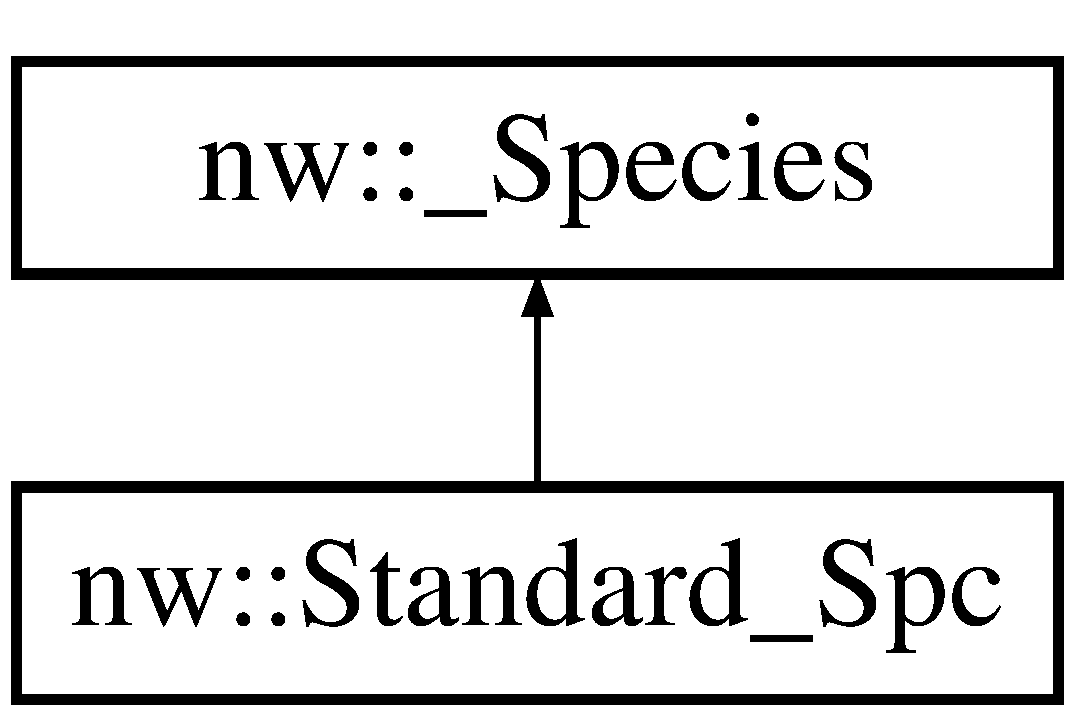
\includegraphics[height=2.000000cm]{da/d48/classnw_1_1_standard___spc}
\end{center}
\end{figure}
\subsection*{Public Member Functions}
\begin{DoxyCompactItemize}
\item 
\hyperlink{classnw_1_1_standard___spc_aba0f0fbe55666cbcf5fbdd8d66f51565}{Standard\+\_\+\+Spc} (long \hyperlink{classnw_1_1___species_ac42dfe1c656c17178a9649093519ebb7}{id}, std\+::string \hyperlink{classnw_1_1___species_a7b8ede09e28941beb48cf27f1247e2f9}{name}, double \hyperlink{classnw_1_1___species_ac66cdd3bdd5be88791e00d063b4e92a2}{initial\+\_\+conc})
\begin{DoxyCompactList}\small\item\em Constructor. \end{DoxyCompactList}\item 
\hyperlink{classnw_1_1_standard___spc_a8113363092a1784829d8f22149d2cef0}{$\sim$\+Standard\+\_\+\+Spc} ()
\begin{DoxyCompactList}\small\item\em Destructor. \end{DoxyCompactList}\item 
long \hyperlink{classnw_1_1_standard___spc_aa1b07cee6c86dd83aa9970c0964d16fc}{get\+\_\+n\+\_\+molecules} ()
\begin{DoxyCompactList}\small\item\em Implementation of the \hyperlink{classnw_1_1___species_a6e3e68477663ff511d75fb24cf01cb9f}{\+\_\+\+Species\+::get\+\_\+n\+\_\+molecules()} method. \end{DoxyCompactList}\item 
void \hyperlink{classnw_1_1_standard___spc_aed4c0ba53c924011269b59a4a5181fe4}{mod\+\_\+n\+\_\+molecules} (long n)
\begin{DoxyCompactList}\small\item\em Implementation of the \hyperlink{classnw_1_1___species_ac7955c9fe040d8cae8f3cae4684ed96b}{\+\_\+\+Species\+::mod\+\_\+n\+\_\+molecules()} method. \end{DoxyCompactList}\item 
\hyperlink{classnw_1_1___species}{\+\_\+\+Species} $\ast$ \hyperlink{classnw_1_1_standard___spc_abc6e6a61ebdcd1e1b917c3e3a5f9cd24}{copy} ()
\begin{DoxyCompactList}\small\item\em Implementation of the \hyperlink{classnw_1_1___species_aea43d96b0b1c9e88953f40fbe58e7f29}{\+\_\+\+Species\+::copy()} method. \end{DoxyCompactList}\end{DoxyCompactItemize}
\subsection*{Additional Inherited Members}


\subsection{Detailed Description}
Basic implementation of a standard moecular species. 

Basic unit of a \hyperlink{classnw_1_1_gillespie___sys}{Gillespie\+\_\+\+Sys}. Every \hyperlink{classnw_1_1___voxel}{\+\_\+\+Voxel} has a state\+\_\+vector that consists of molecular \hyperlink{classnw_1_1___species}{\+\_\+\+Species}. A \hyperlink{classnw_1_1___species}{\+\_\+\+Species} is defined by its current number of molecules, its id and name, and a dirty\+\_\+flag. The dirty flag indicates that the species has been updated during the previous \hyperlink{classnw_1_1___event}{\+\_\+\+Event}. 

\subsection{Constructor \& Destructor Documentation}
\hypertarget{classnw_1_1_standard___spc_aba0f0fbe55666cbcf5fbdd8d66f51565}{\index{nw\+::\+Standard\+\_\+\+Spc@{nw\+::\+Standard\+\_\+\+Spc}!Standard\+\_\+\+Spc@{Standard\+\_\+\+Spc}}
\index{Standard\+\_\+\+Spc@{Standard\+\_\+\+Spc}!nw\+::\+Standard\+\_\+\+Spc@{nw\+::\+Standard\+\_\+\+Spc}}
\subsubsection[{Standard\+\_\+\+Spc}]{\setlength{\rightskip}{0pt plus 5cm}nw\+::\+Standard\+\_\+\+Spc\+::\+Standard\+\_\+\+Spc (
\begin{DoxyParamCaption}
\item[{long}]{id, }
\item[{std\+::string}]{name, }
\item[{double}]{initial\+\_\+conc}
\end{DoxyParamCaption}
)\hspace{0.3cm}{\ttfamily [inline]}}}\label{classnw_1_1_standard___spc_aba0f0fbe55666cbcf5fbdd8d66f51565}


Constructor. 


\begin{DoxyParams}{Parameters}
{\em id} & \hyperlink{classnw_1_1___species}{\+\_\+\+Species} I\+D. \\
\hline
{\em name} & \hyperlink{classnw_1_1___species}{\+\_\+\+Species} name \\
\hline
{\em initial\+\_\+conc} & \hyperlink{classnw_1_1___species}{\+\_\+\+Species} Initial concentration \\
\hline
\end{DoxyParams}

\begin{DoxyCode}
21 :\hyperlink{classnw_1_1___species_af74ef3f4a59f3c8fa9ff6b1acc83be86}{\_Species}(\textcolor{keywordtype}{id},\hyperlink{classnw_1_1___species_a7b8ede09e28941beb48cf27f1247e2f9}{name},\hyperlink{classnw_1_1___species_ac66cdd3bdd5be88791e00d063b4e92a2}{initial\_conc})\{\}
\end{DoxyCode}
\hypertarget{classnw_1_1_standard___spc_a8113363092a1784829d8f22149d2cef0}{\index{nw\+::\+Standard\+\_\+\+Spc@{nw\+::\+Standard\+\_\+\+Spc}!````~Standard\+\_\+\+Spc@{$\sim$\+Standard\+\_\+\+Spc}}
\index{````~Standard\+\_\+\+Spc@{$\sim$\+Standard\+\_\+\+Spc}!nw\+::\+Standard\+\_\+\+Spc@{nw\+::\+Standard\+\_\+\+Spc}}
\subsubsection[{$\sim$\+Standard\+\_\+\+Spc}]{\setlength{\rightskip}{0pt plus 5cm}nw\+::\+Standard\+\_\+\+Spc\+::$\sim$\+Standard\+\_\+\+Spc (
\begin{DoxyParamCaption}
{}
\end{DoxyParamCaption}
)\hspace{0.3cm}{\ttfamily [inline]}}}\label{classnw_1_1_standard___spc_a8113363092a1784829d8f22149d2cef0}


Destructor. 


\begin{DoxyCode}
23 \{\}
\end{DoxyCode}


\subsection{Member Function Documentation}
\hypertarget{classnw_1_1_standard___spc_abc6e6a61ebdcd1e1b917c3e3a5f9cd24}{\index{nw\+::\+Standard\+\_\+\+Spc@{nw\+::\+Standard\+\_\+\+Spc}!copy@{copy}}
\index{copy@{copy}!nw\+::\+Standard\+\_\+\+Spc@{nw\+::\+Standard\+\_\+\+Spc}}
\subsubsection[{copy}]{\setlength{\rightskip}{0pt plus 5cm}{\bf \+\_\+\+Species}$\ast$ nw\+::\+Standard\+\_\+\+Spc\+::copy (
\begin{DoxyParamCaption}
{}
\end{DoxyParamCaption}
)\hspace{0.3cm}{\ttfamily [inline]}, {\ttfamily [virtual]}}}\label{classnw_1_1_standard___spc_abc6e6a61ebdcd1e1b917c3e3a5f9cd24}


Implementation of the \hyperlink{classnw_1_1___species_aea43d96b0b1c9e88953f40fbe58e7f29}{\+\_\+\+Species\+::copy()} method. 



Implements \hyperlink{classnw_1_1___species_aea43d96b0b1c9e88953f40fbe58e7f29}{nw\+::\+\_\+\+Species}.


\begin{DoxyCode}
30                     \{
31         \hyperlink{classnw_1_1___species_af74ef3f4a59f3c8fa9ff6b1acc83be86}{\_Species}* s = \textcolor{keyword}{new} \hyperlink{classnw_1_1_standard___spc_aba0f0fbe55666cbcf5fbdd8d66f51565}{Standard\_Spc}(\textcolor{keywordtype}{id},\hyperlink{classnw_1_1___species_a7b8ede09e28941beb48cf27f1247e2f9}{name},
      \hyperlink{classnw_1_1___species_ac66cdd3bdd5be88791e00d063b4e92a2}{initial\_conc});
32         \textcolor{keywordflow}{return} s;\}
\end{DoxyCode}
\hypertarget{classnw_1_1_standard___spc_aa1b07cee6c86dd83aa9970c0964d16fc}{\index{nw\+::\+Standard\+\_\+\+Spc@{nw\+::\+Standard\+\_\+\+Spc}!get\+\_\+n\+\_\+molecules@{get\+\_\+n\+\_\+molecules}}
\index{get\+\_\+n\+\_\+molecules@{get\+\_\+n\+\_\+molecules}!nw\+::\+Standard\+\_\+\+Spc@{nw\+::\+Standard\+\_\+\+Spc}}
\subsubsection[{get\+\_\+n\+\_\+molecules}]{\setlength{\rightskip}{0pt plus 5cm}long nw\+::\+Standard\+\_\+\+Spc\+::get\+\_\+n\+\_\+molecules (
\begin{DoxyParamCaption}
{}
\end{DoxyParamCaption}
)\hspace{0.3cm}{\ttfamily [inline]}, {\ttfamily [virtual]}}}\label{classnw_1_1_standard___spc_aa1b07cee6c86dd83aa9970c0964d16fc}


Implementation of the \hyperlink{classnw_1_1___species_a6e3e68477663ff511d75fb24cf01cb9f}{\+\_\+\+Species\+::get\+\_\+n\+\_\+molecules()} method. 



Implements \hyperlink{classnw_1_1___species_a6e3e68477663ff511d75fb24cf01cb9f}{nw\+::\+\_\+\+Species}.


\begin{DoxyCode}
25 \{\textcolor{keywordflow}{return} \hyperlink{classnw_1_1___species_af6ae0232b4f994b464a2f69cb022b33f}{n\_molecules};\}
\end{DoxyCode}
\hypertarget{classnw_1_1_standard___spc_aed4c0ba53c924011269b59a4a5181fe4}{\index{nw\+::\+Standard\+\_\+\+Spc@{nw\+::\+Standard\+\_\+\+Spc}!mod\+\_\+n\+\_\+molecules@{mod\+\_\+n\+\_\+molecules}}
\index{mod\+\_\+n\+\_\+molecules@{mod\+\_\+n\+\_\+molecules}!nw\+::\+Standard\+\_\+\+Spc@{nw\+::\+Standard\+\_\+\+Spc}}
\subsubsection[{mod\+\_\+n\+\_\+molecules}]{\setlength{\rightskip}{0pt plus 5cm}void nw\+::\+Standard\+\_\+\+Spc\+::mod\+\_\+n\+\_\+molecules (
\begin{DoxyParamCaption}
\item[{long}]{n}
\end{DoxyParamCaption}
)\hspace{0.3cm}{\ttfamily [inline]}, {\ttfamily [virtual]}}}\label{classnw_1_1_standard___spc_aed4c0ba53c924011269b59a4a5181fe4}


Implementation of the \hyperlink{classnw_1_1___species_ac7955c9fe040d8cae8f3cae4684ed96b}{\+\_\+\+Species\+::mod\+\_\+n\+\_\+molecules()} method. 



Implements \hyperlink{classnw_1_1___species_ac7955c9fe040d8cae8f3cae4684ed96b}{nw\+::\+\_\+\+Species}.


\begin{DoxyCode}
27                                 \{
28         \hyperlink{classnw_1_1___species_af6ae0232b4f994b464a2f69cb022b33f}{n\_molecules} += n; \textcolor{keywordflow}{if}(n!=0)\{\hyperlink{classnw_1_1___species_a79157bae3920ce7bba35e3f75b2aad6f}{dirty\_flag} = \textcolor{keyword}{true};\}\}
\end{DoxyCode}


The documentation for this class was generated from the following file\+:\begin{DoxyCompactItemize}
\item 
Species/\hyperlink{_standard___spc_8h}{Standard\+\_\+\+Spc.\+h}\end{DoxyCompactItemize}

\hypertarget{classnw_1_1_standard___vxl}{\section{nw\+:\+:Standard\+\_\+\+Vxl Class Reference}
\label{classnw_1_1_standard___vxl}\index{nw\+::\+Standard\+\_\+\+Vxl@{nw\+::\+Standard\+\_\+\+Vxl}}
}


Standard voxel implementation.  




{\ttfamily \#include $<$Standard\+\_\+\+Vxl.\+h$>$}

Inheritance diagram for nw\+:\+:Standard\+\_\+\+Vxl\+:\begin{figure}[H]
\begin{center}
\leavevmode
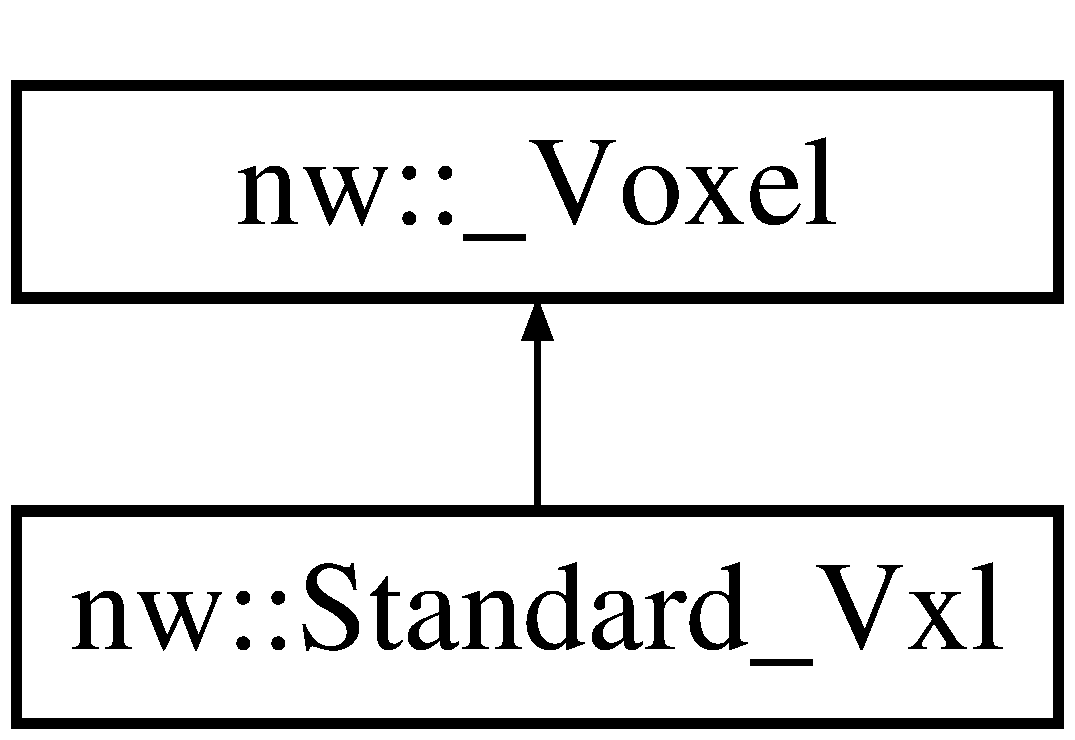
\includegraphics[height=2.000000cm]{d6/de9/classnw_1_1_standard___vxl}
\end{center}
\end{figure}
\subsection*{Public Member Functions}
\begin{DoxyCompactItemize}
\item 
\hyperlink{classnw_1_1_standard___vxl_ad1d02439e7f0cc07201670e1ea71948f}{Standard\+\_\+\+Vxl} (long \hyperlink{classnw_1_1___voxel_a01b73aff9af26230df4c483c5bd81896}{id}, double \hyperlink{classnw_1_1___voxel_ad9c3dbd0ea989af6ba7e1b5e09f6a989}{box\+\_\+length}, \hyperlink{namespacenw_a68aa8285591d78ebfc793c531bd43a23}{Species\+Vector} \hyperlink{classnw_1_1___voxel_a7762f59802c2a0b54bd18acbf803ff34}{state\+\_\+vec})
\begin{DoxyCompactList}\small\item\em Constructor. \end{DoxyCompactList}\item 
\hyperlink{classnw_1_1_standard___vxl_aec0005a231762580af391251e9308c2c}{$\sim$\+Standard\+\_\+\+Vxl} ()
\begin{DoxyCompactList}\small\item\em Destructor. \end{DoxyCompactList}\item 
void \hyperlink{classnw_1_1_standard___vxl_a1d8906f5bbbce6315585959bd1b1a935}{update\+\_\+state} (vector$<$ long $>$)
\begin{DoxyCompactList}\small\item\em Implementation of the \hyperlink{classnw_1_1___voxel_a5842ac3c24bda907204852db0cf46810}{\+\_\+\+Voxel\+::update\+\_\+state()} method. \end{DoxyCompactList}\end{DoxyCompactItemize}
\subsection*{Additional Inherited Members}


\subsection{Detailed Description}
Standard voxel implementation. 

Most importantly it implements the {\ttfamily \hyperlink{classnw_1_1_standard___vxl_a1d8906f5bbbce6315585959bd1b1a935}{update\+\_\+state()}} function of its mother class, so that the state vector (state\+\_\+vec) can be modified by events (in contrast to \hyperlink{classnw_1_1_border___vxl}{Border\+\_\+\+Vxl}). 

\subsection{Constructor \& Destructor Documentation}
\hypertarget{classnw_1_1_standard___vxl_ad1d02439e7f0cc07201670e1ea71948f}{\index{nw\+::\+Standard\+\_\+\+Vxl@{nw\+::\+Standard\+\_\+\+Vxl}!Standard\+\_\+\+Vxl@{Standard\+\_\+\+Vxl}}
\index{Standard\+\_\+\+Vxl@{Standard\+\_\+\+Vxl}!nw\+::\+Standard\+\_\+\+Vxl@{nw\+::\+Standard\+\_\+\+Vxl}}
\subsubsection[{Standard\+\_\+\+Vxl}]{\setlength{\rightskip}{0pt plus 5cm}nw\+::\+Standard\+\_\+\+Vxl\+::\+Standard\+\_\+\+Vxl (
\begin{DoxyParamCaption}
\item[{long}]{id, }
\item[{double}]{box\+\_\+length, }
\item[{{\bf Species\+Vector}}]{state\+\_\+vec}
\end{DoxyParamCaption}
)\hspace{0.3cm}{\ttfamily [inline]}}}\label{classnw_1_1_standard___vxl_ad1d02439e7f0cc07201670e1ea71948f}


Constructor. 


\begin{DoxyParams}{Parameters}
{\em id} & \hyperlink{classnw_1_1___voxel}{\+\_\+\+Voxel} I\+D \\
\hline
{\em box\+\_\+length} & \hyperlink{classnw_1_1___voxel}{\+\_\+\+Voxel} box length \\
\hline
{\em state\+\_\+vec} & \hyperlink{classnw_1_1___voxel}{\+\_\+\+Voxel} state vector \\
\hline
\end{DoxyParams}

\begin{DoxyCode}
22 :\hyperlink{classnw_1_1___voxel_a0622dd383528f5115c6a450b6cbb1b34}{\_Voxel}(\textcolor{keywordtype}{id},\hyperlink{classnw_1_1___voxel_ad9c3dbd0ea989af6ba7e1b5e09f6a989}{box\_length},\hyperlink{classnw_1_1___voxel_a7762f59802c2a0b54bd18acbf803ff34}{state\_vec})\{\}
\end{DoxyCode}
\hypertarget{classnw_1_1_standard___vxl_aec0005a231762580af391251e9308c2c}{\index{nw\+::\+Standard\+\_\+\+Vxl@{nw\+::\+Standard\+\_\+\+Vxl}!````~Standard\+\_\+\+Vxl@{$\sim$\+Standard\+\_\+\+Vxl}}
\index{````~Standard\+\_\+\+Vxl@{$\sim$\+Standard\+\_\+\+Vxl}!nw\+::\+Standard\+\_\+\+Vxl@{nw\+::\+Standard\+\_\+\+Vxl}}
\subsubsection[{$\sim$\+Standard\+\_\+\+Vxl}]{\setlength{\rightskip}{0pt plus 5cm}nw\+::\+Standard\+\_\+\+Vxl\+::$\sim$\+Standard\+\_\+\+Vxl (
\begin{DoxyParamCaption}
{}
\end{DoxyParamCaption}
)\hspace{0.3cm}{\ttfamily [inline]}}}\label{classnw_1_1_standard___vxl_aec0005a231762580af391251e9308c2c}


Destructor. 


\begin{DoxyCode}
24 \{\};
\end{DoxyCode}


\subsection{Member Function Documentation}
\hypertarget{classnw_1_1_standard___vxl_a1d8906f5bbbce6315585959bd1b1a935}{\index{nw\+::\+Standard\+\_\+\+Vxl@{nw\+::\+Standard\+\_\+\+Vxl}!update\+\_\+state@{update\+\_\+state}}
\index{update\+\_\+state@{update\+\_\+state}!nw\+::\+Standard\+\_\+\+Vxl@{nw\+::\+Standard\+\_\+\+Vxl}}
\subsubsection[{update\+\_\+state}]{\setlength{\rightskip}{0pt plus 5cm}void nw\+::\+Standard\+\_\+\+Vxl\+::update\+\_\+state (
\begin{DoxyParamCaption}
\item[{vector$<$ long $>$}]{sc\+\_\+vec}
\end{DoxyParamCaption}
)\hspace{0.3cm}{\ttfamily [virtual]}}}\label{classnw_1_1_standard___vxl_a1d8906f5bbbce6315585959bd1b1a935}


Implementation of the \hyperlink{classnw_1_1___voxel_a5842ac3c24bda907204852db0cf46810}{\+\_\+\+Voxel\+::update\+\_\+state()} method. 


\begin{DoxyParams}{Parameters}
{\em sc\+\_\+vec} & State change vector of firing event \\
\hline
\end{DoxyParams}


Implements \hyperlink{classnw_1_1___voxel_a5842ac3c24bda907204852db0cf46810}{nw\+::\+\_\+\+Voxel}.


\begin{DoxyCode}
8 \{
9     \textcolor{keywordflow}{if} (sc\_vec.size() == \hyperlink{classnw_1_1___voxel_a7762f59802c2a0b54bd18acbf803ff34}{state\_vec}.size()) \{
10     \textcolor{comment}{//  update the state vector of voxel using the assigned state change vector (usually called by an
       event)}
11         \textcolor{keywordflow}{for} (\textcolor{keywordtype}{size\_t} i = 0; i < \hyperlink{classnw_1_1___voxel_a7762f59802c2a0b54bd18acbf803ff34}{state\_vec}.size(); ++i) \{
12             \hyperlink{classnw_1_1___voxel_a7762f59802c2a0b54bd18acbf803ff34}{state\_vec}[i]->mod\_n\_molecules(sc\_vec[i]);
13         \}
14         this->\hyperlink{classnw_1_1___voxel_a9c331fe7c0fd8691ef0124f33809764f}{dirty\_flag} = \textcolor{keyword}{true};
15     \} \textcolor{keywordflow}{else} \{
16     \textcolor{comment}{//  Debug information: Throw error if sc\_vec.size() != state\_vec}
17         cout << \textcolor{stringliteral}{"ERROR: state change vector and state vector differ in size"};
18     \}
19 \}
\end{DoxyCode}


The documentation for this class was generated from the following files\+:\begin{DoxyCompactItemize}
\item 
Voxel/\hyperlink{_standard___vxl_8h}{Standard\+\_\+\+Vxl.\+h}\item 
Voxel/\hyperlink{_standard___vxl_8cpp}{Standard\+\_\+\+Vxl.\+cpp}\end{DoxyCompactItemize}

\hypertarget{classnw_1_1_sub_unit_switch___rct___evt}{\section{nw\+:\+:Sub\+Unit\+Switch\+\_\+\+Rct\+\_\+\+Evt Class Reference}
\label{classnw_1_1_sub_unit_switch___rct___evt}\index{nw\+::\+Sub\+Unit\+Switch\+\_\+\+Rct\+\_\+\+Evt@{nw\+::\+Sub\+Unit\+Switch\+\_\+\+Rct\+\_\+\+Evt}}
}


Subunit switch reaction event.  




{\ttfamily \#include $<$Sub\+Unit\+Switch\+\_\+\+Rct\+\_\+\+Evt.\+h$>$}

Inheritance diagram for nw\+:\+:Sub\+Unit\+Switch\+\_\+\+Rct\+\_\+\+Evt\+:\begin{figure}[H]
\begin{center}
\leavevmode
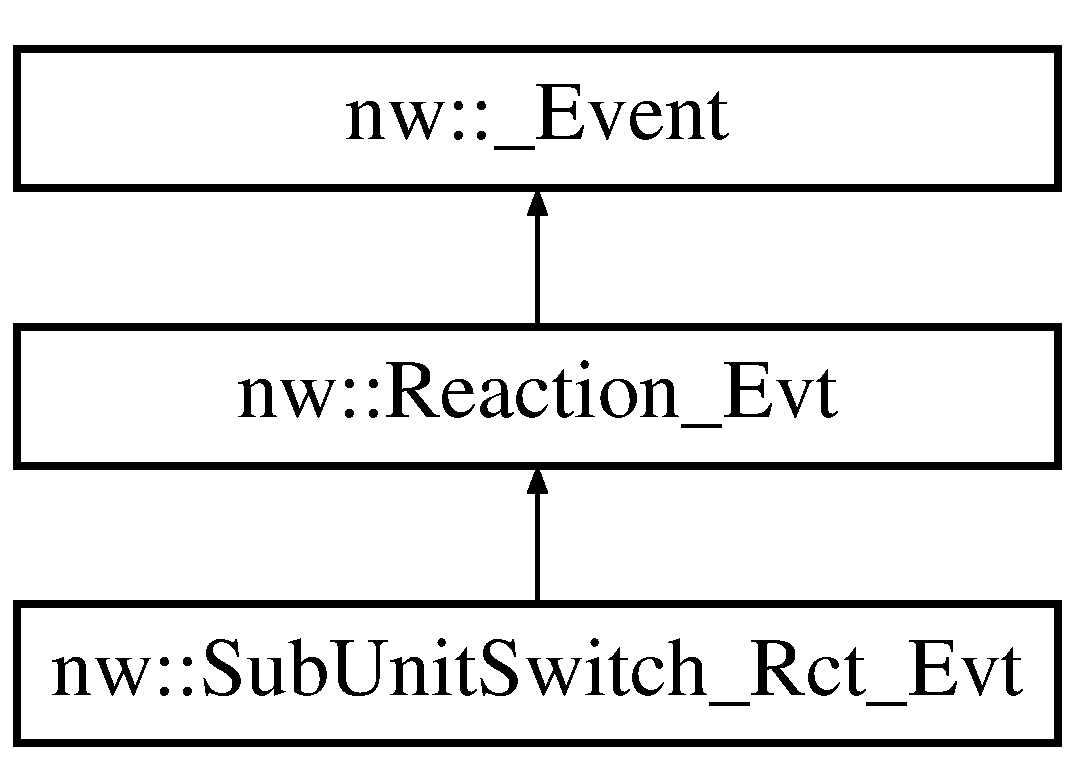
\includegraphics[height=3.000000cm]{d1/d63/classnw_1_1_sub_unit_switch___rct___evt}
\end{center}
\end{figure}
\subsection*{Public Member Functions}
\begin{DoxyCompactItemize}
\item 
\hyperlink{classnw_1_1_sub_unit_switch___rct___evt_a77796138fe4514288417f95dcc053f79}{Sub\+Unit\+Switch\+\_\+\+Rct\+\_\+\+Evt} (long \hyperlink{classnw_1_1___event_a8f7ce287f596266dd763ec7db2f74090}{id}, string \hyperlink{classnw_1_1___event_ab4f50a54039cd4957bdca55049178562}{name}, double \hyperlink{classnw_1_1___event_afca0ae816e9834add07db8e9a6618faa}{k}, vector$<$ long $>$ \hyperlink{classnw_1_1___event_a560c8b6f9954a43f5d5f80204473b64d}{sc\+\_\+vec}, long \hyperlink{classnw_1_1_sub_unit_switch___rct___evt_a3f14cca01fc1645696666330a7354865}{act\+\_\+su\+\_\+id}, long \hyperlink{classnw_1_1_sub_unit_switch___rct___evt_a7d1c65995bc49d7e6e625aa090325af1}{ch\+\_\+spc\+\_\+id}, \hyperlink{namespacenw_ad7146b8b5a9de9be416847f41135722c}{Voxel\+Vector} vvc, \hyperlink{classnw_1_1_uni___rnd}{Uni\+\_\+\+Rnd} $\ast$\hyperlink{classnw_1_1___event_af92482aeea55562560573ecccd5ab108}{rg})
\begin{DoxyCompactList}\small\item\em Constructor. \end{DoxyCompactList}\item 
virtual \hyperlink{classnw_1_1_sub_unit_switch___rct___evt_a054845f5f9892951bfe04ffd57563243}{$\sim$\+Sub\+Unit\+Switch\+\_\+\+Rct\+\_\+\+Evt} ()
\item 
void \hyperlink{classnw_1_1_sub_unit_switch___rct___evt_ab89891fae9287edc9d9a215788706093}{execute} ()
\begin{DoxyCompactList}\small\item\em Implementation of the \hyperlink{classnw_1_1___event_aa022418fb765582a053ac75cbc3436d6}{\+\_\+\+Event\+::execute()} method. \end{DoxyCompactList}\end{DoxyCompactItemize}
\subsection*{Private Member Functions}
\begin{DoxyCompactItemize}
\item 
void \hyperlink{classnw_1_1_sub_unit_switch___rct___evt_a616d644628a7b4ada1c64733c601354f}{update\+\_\+\+Channel\+\_\+\+Spc} ()
\begin{DoxyCompactList}\small\item\em Updates the referenced channel Species every time this event is executed. \end{DoxyCompactList}\end{DoxyCompactItemize}
\subsection*{Private Attributes}
\begin{DoxyCompactItemize}
\item 
\hyperlink{classnw_1_1_channel___spc}{Channel\+\_\+\+Spc} $\ast$ \hyperlink{classnw_1_1_sub_unit_switch___rct___evt_a260fabe9e3e1d8b79c3c80bb987716a5}{chs}
\begin{DoxyCompactList}\small\item\em Pointer to the downcasted \hyperlink{classnw_1_1_channel___spc}{Channel\+\_\+\+Spc}. \end{DoxyCompactList}\item 
long \hyperlink{classnw_1_1_sub_unit_switch___rct___evt_a3f14cca01fc1645696666330a7354865}{act\+\_\+su\+\_\+id}
\begin{DoxyCompactList}\small\item\em \hyperlink{classnw_1_1___species}{\+\_\+\+Species} id of the activated subunit \end{DoxyCompactList}\item 
long \hyperlink{classnw_1_1_sub_unit_switch___rct___evt_a7d1c65995bc49d7e6e625aa090325af1}{ch\+\_\+spc\+\_\+id}
\begin{DoxyCompactList}\small\item\em \hyperlink{classnw_1_1___species}{\+\_\+\+Species} id of the \hyperlink{classnw_1_1_channel___spc}{Channel\+\_\+\+Spc} \end{DoxyCompactList}\end{DoxyCompactItemize}
\subsection*{Additional Inherited Members}


\subsection{Detailed Description}
Subunit switch reaction event. 

Coordinates reaction events that change the state of a subunit. Whenever a subunit becomes activated the Channl\+\_\+\+Spc has to be notified, since the number of open channels depends on the number of active subunits. 

\subsection{Constructor \& Destructor Documentation}
\hypertarget{classnw_1_1_sub_unit_switch___rct___evt_a77796138fe4514288417f95dcc053f79}{\index{nw\+::\+Sub\+Unit\+Switch\+\_\+\+Rct\+\_\+\+Evt@{nw\+::\+Sub\+Unit\+Switch\+\_\+\+Rct\+\_\+\+Evt}!Sub\+Unit\+Switch\+\_\+\+Rct\+\_\+\+Evt@{Sub\+Unit\+Switch\+\_\+\+Rct\+\_\+\+Evt}}
\index{Sub\+Unit\+Switch\+\_\+\+Rct\+\_\+\+Evt@{Sub\+Unit\+Switch\+\_\+\+Rct\+\_\+\+Evt}!nw\+::\+Sub\+Unit\+Switch\+\_\+\+Rct\+\_\+\+Evt@{nw\+::\+Sub\+Unit\+Switch\+\_\+\+Rct\+\_\+\+Evt}}
\subsubsection[{Sub\+Unit\+Switch\+\_\+\+Rct\+\_\+\+Evt}]{\setlength{\rightskip}{0pt plus 5cm}nw\+::\+Sub\+Unit\+Switch\+\_\+\+Rct\+\_\+\+Evt\+::\+Sub\+Unit\+Switch\+\_\+\+Rct\+\_\+\+Evt (
\begin{DoxyParamCaption}
\item[{long}]{id, }
\item[{string}]{name, }
\item[{double}]{k, }
\item[{vector$<$ long $>$}]{sc\+\_\+vec, }
\item[{long}]{act\+\_\+su\+\_\+id, }
\item[{long}]{ch\+\_\+spc\+\_\+id, }
\item[{{\bf Voxel\+Vector}}]{vvc, }
\item[{{\bf Uni\+\_\+\+Rnd} $\ast$}]{rg}
\end{DoxyParamCaption}
)\hspace{0.3cm}{\ttfamily [inline]}}}\label{classnw_1_1_sub_unit_switch___rct___evt_a77796138fe4514288417f95dcc053f79}


Constructor. 


\begin{DoxyParams}{Parameters}
{\em id} & \hyperlink{classnw_1_1___event}{\+\_\+\+Event} I\+D \\
\hline
{\em name} & \hyperlink{classnw_1_1___event}{\+\_\+\+Event} name \\
\hline
{\em k} & \hyperlink{classnw_1_1___event}{\+\_\+\+Event} rate constant \\
\hline
{\em vvc} & \hyperlink{classnw_1_1___event}{\+\_\+\+Event} voxel vector \\
\hline
{\em sc\+\_\+vec} & \hyperlink{classnw_1_1_reaction___evt}{Reaction\+\_\+\+Evt} state change vector \\
\hline
{\em rg} & \hyperlink{classnw_1_1___event}{\+\_\+\+Event} pointer to a Random\+\_\+\+Generator. \\
\hline
{\em act\+\_\+su\+\_\+id} & Active subunit id \\
\hline
{\em ch\+\_\+spc\+\_\+id} & Channel species id \\
\hline
\end{DoxyParams}

\begin{DoxyCode}
35                                                                          :
36                                 \hyperlink{classnw_1_1_reaction___evt_a582f3c60366d15e89fdd613abe4bd86d}{Reaction\_Evt}(\textcolor{keywordtype}{id}, \hyperlink{classnw_1_1___event_ab4f50a54039cd4957bdca55049178562}{name}, \hyperlink{classnw_1_1___event_afca0ae816e9834add07db8e9a6618faa}{k} ,
      \hyperlink{classnw_1_1___event_a560c8b6f9954a43f5d5f80204473b64d}{sc\_vec},vvc,\hyperlink{classnw_1_1___event_af92482aeea55562560573ecccd5ab108}{rg})\{
37         this->\hyperlink{classnw_1_1_sub_unit_switch___rct___evt_a3f14cca01fc1645696666330a7354865}{act\_su\_id} = \hyperlink{classnw_1_1_sub_unit_switch___rct___evt_a3f14cca01fc1645696666330a7354865}{act\_su\_id};
38         this->\hyperlink{classnw_1_1_sub_unit_switch___rct___evt_a7d1c65995bc49d7e6e625aa090325af1}{ch\_spc\_id} = \hyperlink{classnw_1_1_sub_unit_switch___rct___evt_a7d1c65995bc49d7e6e625aa090325af1}{ch\_spc\_id};
39     \}
\end{DoxyCode}
\hypertarget{classnw_1_1_sub_unit_switch___rct___evt_a054845f5f9892951bfe04ffd57563243}{\index{nw\+::\+Sub\+Unit\+Switch\+\_\+\+Rct\+\_\+\+Evt@{nw\+::\+Sub\+Unit\+Switch\+\_\+\+Rct\+\_\+\+Evt}!````~Sub\+Unit\+Switch\+\_\+\+Rct\+\_\+\+Evt@{$\sim$\+Sub\+Unit\+Switch\+\_\+\+Rct\+\_\+\+Evt}}
\index{````~Sub\+Unit\+Switch\+\_\+\+Rct\+\_\+\+Evt@{$\sim$\+Sub\+Unit\+Switch\+\_\+\+Rct\+\_\+\+Evt}!nw\+::\+Sub\+Unit\+Switch\+\_\+\+Rct\+\_\+\+Evt@{nw\+::\+Sub\+Unit\+Switch\+\_\+\+Rct\+\_\+\+Evt}}
\subsubsection[{$\sim$\+Sub\+Unit\+Switch\+\_\+\+Rct\+\_\+\+Evt}]{\setlength{\rightskip}{0pt plus 5cm}virtual nw\+::\+Sub\+Unit\+Switch\+\_\+\+Rct\+\_\+\+Evt\+::$\sim$\+Sub\+Unit\+Switch\+\_\+\+Rct\+\_\+\+Evt (
\begin{DoxyParamCaption}
{}
\end{DoxyParamCaption}
)\hspace{0.3cm}{\ttfamily [inline]}, {\ttfamily [virtual]}}}\label{classnw_1_1_sub_unit_switch___rct___evt_a054845f5f9892951bfe04ffd57563243}
Destructor 
\begin{DoxyCode}
41 \{\};
\end{DoxyCode}


\subsection{Member Function Documentation}
\hypertarget{classnw_1_1_sub_unit_switch___rct___evt_ab89891fae9287edc9d9a215788706093}{\index{nw\+::\+Sub\+Unit\+Switch\+\_\+\+Rct\+\_\+\+Evt@{nw\+::\+Sub\+Unit\+Switch\+\_\+\+Rct\+\_\+\+Evt}!execute@{execute}}
\index{execute@{execute}!nw\+::\+Sub\+Unit\+Switch\+\_\+\+Rct\+\_\+\+Evt@{nw\+::\+Sub\+Unit\+Switch\+\_\+\+Rct\+\_\+\+Evt}}
\subsubsection[{execute}]{\setlength{\rightskip}{0pt plus 5cm}void Sub\+Unit\+Switch\+\_\+\+Rct\+\_\+\+Evt\+::execute (
\begin{DoxyParamCaption}
{}
\end{DoxyParamCaption}
)\hspace{0.3cm}{\ttfamily [virtual]}}}\label{classnw_1_1_sub_unit_switch___rct___evt_ab89891fae9287edc9d9a215788706093}


Implementation of the \hyperlink{classnw_1_1___event_aa022418fb765582a053ac75cbc3436d6}{\+\_\+\+Event\+::execute()} method. 

Whenever a subunit switch reaction event occurs, a channel subunit switches between an activated state and an inactivated state. This affects the state of a channel and thus needs to be communicated. This happens via a typecast of the \hyperlink{classnw_1_1___species}{\+\_\+\+Species} pointer to its more specific derivative \hyperlink{classnw_1_1_channel___spc}{Channel\+\_\+\+Spc} (identified via the ch\+\_\+spc\+\_\+id attribute). The result of the typecast allows for the call of public functions that are only accessible via the \hyperlink{classnw_1_1_channel___spc}{Channel\+\_\+\+Spc} interface. Consequently the function \hyperlink{classnw_1_1_channel___spc_ab5176b0d9aed2ac68a142488d11b5e81}{Channel\+\_\+\+Spc\+::activate\+\_\+\+Subunit()} or \hyperlink{classnw_1_1_channel___spc_a190172435ab84f9210ae027d06aae81a}{Channel\+\_\+\+Spc\+::inactivate\+\_\+\+Subunit()} can be called. 

Reimplemented from \hyperlink{classnw_1_1_reaction___evt_aec2fb342726ef17255ebf406a7c74392}{nw\+::\+Reaction\+\_\+\+Evt}.


\begin{DoxyCode}
8                                    \{
9 
10     \textcolor{keywordflow}{try}\{
11 \textcolor{comment}{//      execute event by using the state change vector}
12         \hyperlink{classnw_1_1___event_a6351b58d94923ed58e0b2cf6c9445d2e}{tv\_vec}[\hyperlink{classnw_1_1___event_a7864559e204c087306e3becb5b81fb26}{nextVoxel}].v->update\_state(\hyperlink{classnw_1_1___event_a560c8b6f9954a43f5d5f80204473b64d}{sc\_vec});
13 
14 \textcolor{comment}{//      set dirty flag to indicate that dependent events have to be updated properly}
15         \textcolor{keywordflow}{for}(\textcolor{keywordtype}{long} i = 0; i < (long)\hyperlink{classnw_1_1___event_a3f87b2dff69d07977f0a5e10936f38f6}{dep\_list}.size(); i++)\{
16             \hyperlink{classnw_1_1___event_a3f87b2dff69d07977f0a5e10936f38f6}{dep\_list}[i]->set\_flag(\textcolor{keyword}{true});
17         \}
18 
19 \textcolor{comment}{//      update the activation states of the subunits of chs}
20         \hyperlink{classnw_1_1_sub_unit_switch___rct___evt_a260fabe9e3e1d8b79c3c80bb987716a5}{chs} = \textcolor{keyword}{dynamic\_cast<}\hyperlink{classnw_1_1_channel___spc}{Channel\_Spc}*\textcolor{keyword}{>}(\hyperlink{classnw_1_1___event_a6351b58d94923ed58e0b2cf6c9445d2e}{tv\_vec}[\hyperlink{classnw_1_1___event_a7864559e204c087306e3becb5b81fb26}{nextVoxel}].v->get\_state\_vec()
      ->at(\hyperlink{classnw_1_1_sub_unit_switch___rct___evt_a7d1c65995bc49d7e6e625aa090325af1}{ch\_spc\_id}));  \textcolor{comment}{// cave: downcasting (\_Species->Channel\_Spc)...}
21         \hyperlink{classnw_1_1_sub_unit_switch___rct___evt_a616d644628a7b4ada1c64733c601354f}{update\_Channel\_Spc}();
22     \}
23     \textcolor{keywordflow}{catch}(exception& e)\{
24         cout << \textcolor{stringliteral}{"SubuintSwitch\_Rct\_evt::execute(): "} << e.what();
25         \}
26     \}
\end{DoxyCode}
\hypertarget{classnw_1_1_sub_unit_switch___rct___evt_a616d644628a7b4ada1c64733c601354f}{\index{nw\+::\+Sub\+Unit\+Switch\+\_\+\+Rct\+\_\+\+Evt@{nw\+::\+Sub\+Unit\+Switch\+\_\+\+Rct\+\_\+\+Evt}!update\+\_\+\+Channel\+\_\+\+Spc@{update\+\_\+\+Channel\+\_\+\+Spc}}
\index{update\+\_\+\+Channel\+\_\+\+Spc@{update\+\_\+\+Channel\+\_\+\+Spc}!nw\+::\+Sub\+Unit\+Switch\+\_\+\+Rct\+\_\+\+Evt@{nw\+::\+Sub\+Unit\+Switch\+\_\+\+Rct\+\_\+\+Evt}}
\subsubsection[{update\+\_\+\+Channel\+\_\+\+Spc}]{\setlength{\rightskip}{0pt plus 5cm}void Sub\+Unit\+Switch\+\_\+\+Rct\+\_\+\+Evt\+::update\+\_\+\+Channel\+\_\+\+Spc (
\begin{DoxyParamCaption}
{}
\end{DoxyParamCaption}
)\hspace{0.3cm}{\ttfamily [private]}}}\label{classnw_1_1_sub_unit_switch___rct___evt_a616d644628a7b4ada1c64733c601354f}


Updates the referenced channel Species every time this event is executed. 


\begin{DoxyCode}
28                                               \{
29 
30     \textcolor{keywordflow}{if} (\hyperlink{classnw_1_1___event_a560c8b6f9954a43f5d5f80204473b64d}{sc\_vec}.at(\hyperlink{classnw_1_1_sub_unit_switch___rct___evt_a3f14cca01fc1645696666330a7354865}{act\_su\_id}) > 0)\{
31         \textcolor{keywordtype}{long} r\_chid = (long)(\hyperlink{classnw_1_1___event_af92482aeea55562560573ecccd5ab108}{rg}->\hyperlink{classnw_1_1_uni___rnd_ad7883ef0ce4c591612bcb41678104773}{get\_Uni\_Rnd}() * \hyperlink{classnw_1_1_sub_unit_switch___rct___evt_a260fabe9e3e1d8b79c3c80bb987716a5}{chs}->
      \hyperlink{classnw_1_1_channel___spc_aecd939824b8d2a275cbe360f60ae4a2d}{get\_n\_Activable\_Ch}());
32         \hyperlink{classnw_1_1_sub_unit_switch___rct___evt_a260fabe9e3e1d8b79c3c80bb987716a5}{chs}->\hyperlink{classnw_1_1_channel___spc_ab5176b0d9aed2ac68a142488d11b5e81}{activate\_Subunit}(r\_chid);
33     \}\textcolor{keywordflow}{else} \textcolor{keywordflow}{if}(\hyperlink{classnw_1_1___event_a560c8b6f9954a43f5d5f80204473b64d}{sc\_vec}.at(\hyperlink{classnw_1_1_sub_unit_switch___rct___evt_a3f14cca01fc1645696666330a7354865}{act\_su\_id}) < 0)\{
34         \textcolor{keywordtype}{long} r\_chid = (long)(\hyperlink{classnw_1_1___event_af92482aeea55562560573ecccd5ab108}{rg}->\hyperlink{classnw_1_1_uni___rnd_ad7883ef0ce4c591612bcb41678104773}{get\_Uni\_Rnd}() * \hyperlink{classnw_1_1_sub_unit_switch___rct___evt_a260fabe9e3e1d8b79c3c80bb987716a5}{chs}->
      \hyperlink{classnw_1_1_channel___spc_a99c02ea4a145d6531ed2328de073fb37}{get\_n\_Inactivable\_Ch}());
35         \hyperlink{classnw_1_1_sub_unit_switch___rct___evt_a260fabe9e3e1d8b79c3c80bb987716a5}{chs}->\hyperlink{classnw_1_1_channel___spc_a190172435ab84f9210ae027d06aae81a}{inactivate\_Subunit}(r\_chid);
36     \}\textcolor{keywordflow}{else}\{
37         cout << \textcolor{stringliteral}{"ERROR: The SubUnitActSwitch\_Rct\_Evt state change vector doesn't suit the assigned
       active\_subUnit\_Species\_ID. Please check your input!"} << endl;
38     \}
39 \}
\end{DoxyCode}


\subsection{Member Data Documentation}
\hypertarget{classnw_1_1_sub_unit_switch___rct___evt_a3f14cca01fc1645696666330a7354865}{\index{nw\+::\+Sub\+Unit\+Switch\+\_\+\+Rct\+\_\+\+Evt@{nw\+::\+Sub\+Unit\+Switch\+\_\+\+Rct\+\_\+\+Evt}!act\+\_\+su\+\_\+id@{act\+\_\+su\+\_\+id}}
\index{act\+\_\+su\+\_\+id@{act\+\_\+su\+\_\+id}!nw\+::\+Sub\+Unit\+Switch\+\_\+\+Rct\+\_\+\+Evt@{nw\+::\+Sub\+Unit\+Switch\+\_\+\+Rct\+\_\+\+Evt}}
\subsubsection[{act\+\_\+su\+\_\+id}]{\setlength{\rightskip}{0pt plus 5cm}long nw\+::\+Sub\+Unit\+Switch\+\_\+\+Rct\+\_\+\+Evt\+::act\+\_\+su\+\_\+id\hspace{0.3cm}{\ttfamily [private]}}}\label{classnw_1_1_sub_unit_switch___rct___evt_a3f14cca01fc1645696666330a7354865}


\hyperlink{classnw_1_1___species}{\+\_\+\+Species} id of the activated subunit 

\hypertarget{classnw_1_1_sub_unit_switch___rct___evt_a7d1c65995bc49d7e6e625aa090325af1}{\index{nw\+::\+Sub\+Unit\+Switch\+\_\+\+Rct\+\_\+\+Evt@{nw\+::\+Sub\+Unit\+Switch\+\_\+\+Rct\+\_\+\+Evt}!ch\+\_\+spc\+\_\+id@{ch\+\_\+spc\+\_\+id}}
\index{ch\+\_\+spc\+\_\+id@{ch\+\_\+spc\+\_\+id}!nw\+::\+Sub\+Unit\+Switch\+\_\+\+Rct\+\_\+\+Evt@{nw\+::\+Sub\+Unit\+Switch\+\_\+\+Rct\+\_\+\+Evt}}
\subsubsection[{ch\+\_\+spc\+\_\+id}]{\setlength{\rightskip}{0pt plus 5cm}long nw\+::\+Sub\+Unit\+Switch\+\_\+\+Rct\+\_\+\+Evt\+::ch\+\_\+spc\+\_\+id\hspace{0.3cm}{\ttfamily [private]}}}\label{classnw_1_1_sub_unit_switch___rct___evt_a7d1c65995bc49d7e6e625aa090325af1}


\hyperlink{classnw_1_1___species}{\+\_\+\+Species} id of the \hyperlink{classnw_1_1_channel___spc}{Channel\+\_\+\+Spc} 

\hypertarget{classnw_1_1_sub_unit_switch___rct___evt_a260fabe9e3e1d8b79c3c80bb987716a5}{\index{nw\+::\+Sub\+Unit\+Switch\+\_\+\+Rct\+\_\+\+Evt@{nw\+::\+Sub\+Unit\+Switch\+\_\+\+Rct\+\_\+\+Evt}!chs@{chs}}
\index{chs@{chs}!nw\+::\+Sub\+Unit\+Switch\+\_\+\+Rct\+\_\+\+Evt@{nw\+::\+Sub\+Unit\+Switch\+\_\+\+Rct\+\_\+\+Evt}}
\subsubsection[{chs}]{\setlength{\rightskip}{0pt plus 5cm}{\bf Channel\+\_\+\+Spc}$\ast$ nw\+::\+Sub\+Unit\+Switch\+\_\+\+Rct\+\_\+\+Evt\+::chs\hspace{0.3cm}{\ttfamily [private]}}}\label{classnw_1_1_sub_unit_switch___rct___evt_a260fabe9e3e1d8b79c3c80bb987716a5}


Pointer to the downcasted \hyperlink{classnw_1_1_channel___spc}{Channel\+\_\+\+Spc}. 



The documentation for this class was generated from the following files\+:\begin{DoxyCompactItemize}
\item 
Events/\hyperlink{_sub_unit_switch___rct___evt_8h}{Sub\+Unit\+Switch\+\_\+\+Rct\+\_\+\+Evt.\+h}\item 
Events/\hyperlink{_sub_unit_switch___rct___evt_8cpp}{Sub\+Unit\+Switch\+\_\+\+Rct\+\_\+\+Evt.\+cpp}\end{DoxyCompactItemize}

\hypertarget{structnw_1_1___event_1_1tv__struct}{\section{nw\+:\+:\+\_\+\+Event\+:\+:tv\+\_\+struct Struct Reference}
\label{structnw_1_1___event_1_1tv__struct}\index{nw\+::\+\_\+\+Event\+::tv\+\_\+struct@{nw\+::\+\_\+\+Event\+::tv\+\_\+struct}}
}


tau-\/voxel-\/structure (\hyperlink{structnw_1_1___event_1_1tv__struct}{tv\+\_\+struct}) is a structure that associates a tau value with a \hyperlink{classnw_1_1___voxel}{\+\_\+\+Voxel}.  




{\ttfamily \#include $<$\+\_\+\+Event.\+h$>$}

\subsection*{Public Attributes}
\begin{DoxyCompactItemize}
\item 
\hyperlink{classnw_1_1___voxel}{\+\_\+\+Voxel} $\ast$ \hyperlink{structnw_1_1___event_1_1tv__struct_af3cef61890dbf9b568baad7c2532ed56}{v}
\begin{DoxyCompactList}\small\item\em pointer to an existing voxel \end{DoxyCompactList}\item 
double \hyperlink{structnw_1_1___event_1_1tv__struct_a60486108e732f06bdb4bc5775e875c37}{t}
\begin{DoxyCompactList}\small\item\em corresponding tau value \end{DoxyCompactList}\end{DoxyCompactItemize}


\subsection{Detailed Description}
tau-\/voxel-\/structure (\hyperlink{structnw_1_1___event_1_1tv__struct}{tv\+\_\+struct}) is a structure that associates a tau value with a \hyperlink{classnw_1_1___voxel}{\+\_\+\+Voxel}. 

{\ttfamily v} points to a \hyperlink{classnw_1_1___voxel}{\+\_\+\+Voxel}, while {\ttfamily t} is the corresponding tau value. It further overloads the {\ttfamily $<$} operator to implement the 'smaller than' operation of two tv\+\_\+structs based on their tau value. 

\subsection{Member Data Documentation}
\hypertarget{structnw_1_1___event_1_1tv__struct_a60486108e732f06bdb4bc5775e875c37}{\index{nw\+::\+\_\+\+Event\+::tv\+\_\+struct@{nw\+::\+\_\+\+Event\+::tv\+\_\+struct}!t@{t}}
\index{t@{t}!nw\+::\+\_\+\+Event\+::tv\+\_\+struct@{nw\+::\+\_\+\+Event\+::tv\+\_\+struct}}
\subsubsection[{t}]{\setlength{\rightskip}{0pt plus 5cm}double nw\+::\+\_\+\+Event\+::tv\+\_\+struct\+::t}}\label{structnw_1_1___event_1_1tv__struct_a60486108e732f06bdb4bc5775e875c37}


corresponding tau value 

\hypertarget{structnw_1_1___event_1_1tv__struct_af3cef61890dbf9b568baad7c2532ed56}{\index{nw\+::\+\_\+\+Event\+::tv\+\_\+struct@{nw\+::\+\_\+\+Event\+::tv\+\_\+struct}!v@{v}}
\index{v@{v}!nw\+::\+\_\+\+Event\+::tv\+\_\+struct@{nw\+::\+\_\+\+Event\+::tv\+\_\+struct}}
\subsubsection[{v}]{\setlength{\rightskip}{0pt plus 5cm}{\bf \+\_\+\+Voxel}$\ast$ nw\+::\+\_\+\+Event\+::tv\+\_\+struct\+::v}}\label{structnw_1_1___event_1_1tv__struct_af3cef61890dbf9b568baad7c2532ed56}


pointer to an existing voxel 



The documentation for this struct was generated from the following file\+:\begin{DoxyCompactItemize}
\item 
Events/\hyperlink{___event_8h}{\+\_\+\+Event.\+h}\end{DoxyCompactItemize}

\hypertarget{classnw_1_1_uni___rnd}{\section{nw\+:\+:Uni\+\_\+\+Rnd Class Reference}
\label{classnw_1_1_uni___rnd}\index{nw\+::\+Uni\+\_\+\+Rnd@{nw\+::\+Uni\+\_\+\+Rnd}}
}


\char`\"{}\+Minimal\char`\"{} random number generator of Park and Miller  




{\ttfamily \#include $<$Uni\+\_\+\+Rnd.\+h$>$}

Inheritance diagram for nw\+:\+:Uni\+\_\+\+Rnd\+:\begin{figure}[H]
\begin{center}
\leavevmode
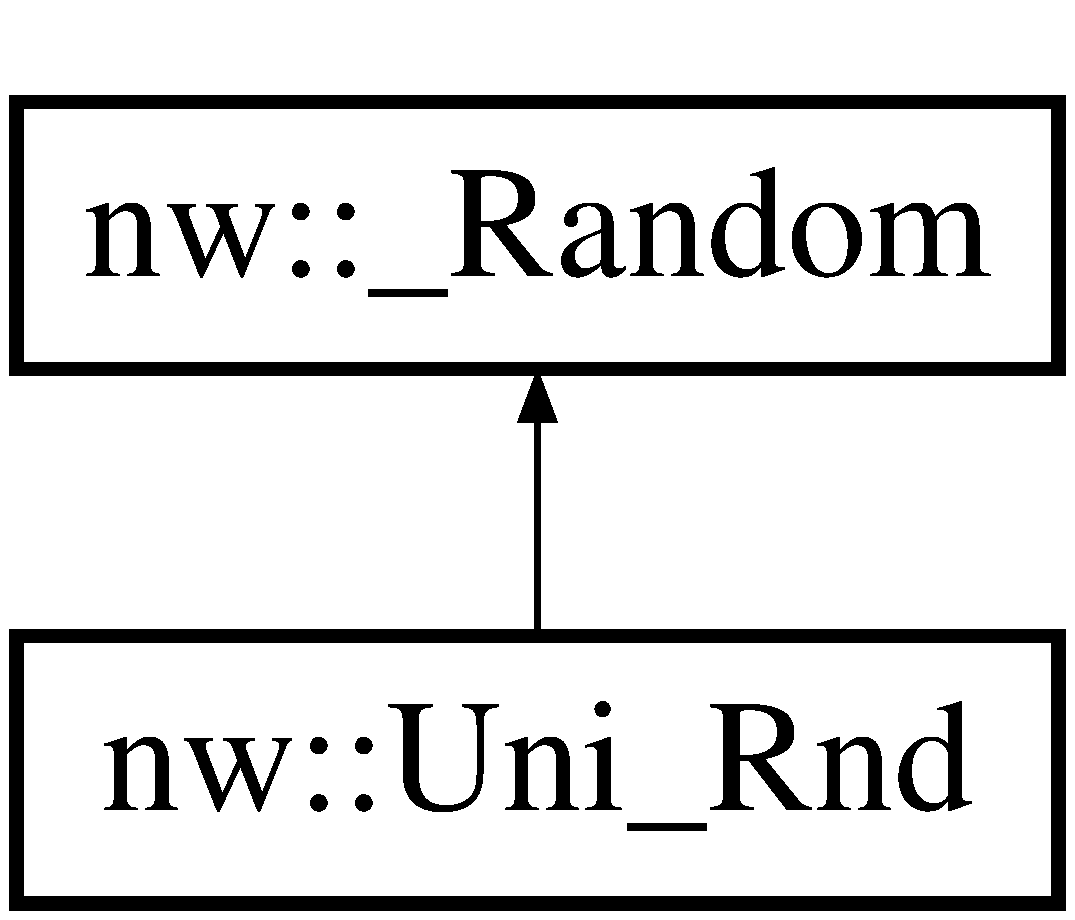
\includegraphics[height=2.000000cm]{d3/dc1/classnw_1_1_uni___rnd}
\end{center}
\end{figure}
\subsection*{Public Member Functions}
\begin{DoxyCompactItemize}
\item 
\hyperlink{classnw_1_1_uni___rnd_ac25386221e6f2da28eb74445c5378b6e}{Uni\+\_\+\+Rnd} ()
\begin{DoxyCompactList}\small\item\em Seed random generator with current time. \end{DoxyCompactList}\item 
double \hyperlink{classnw_1_1_uni___rnd_ad7883ef0ce4c591612bcb41678104773}{get\+\_\+\+Uni\+\_\+\+Rnd} ()
\begin{DoxyCompactList}\small\item\em Implementation of the \hyperlink{classnw_1_1___random_a943da227bd614e34718967a0521a51d1}{\+\_\+\+Random\+::get\+\_\+\+Uni\+\_\+\+Rnd()} method. \end{DoxyCompactList}\end{DoxyCompactItemize}
\subsection*{Private Member Functions}
\begin{DoxyCompactItemize}
\item 
double \hyperlink{classnw_1_1_uni___rnd_a1599d3ea8e72738bbfbad814e9e233ac}{uni\+\_\+\+Rnd} (long $\ast$)
\begin{DoxyCompactList}\small\item\em generates uniform random variable \end{DoxyCompactList}\end{DoxyCompactItemize}
\subsection*{Private Attributes}
\begin{DoxyCompactItemize}
\item 
long \hyperlink{classnw_1_1_uni___rnd_a0b5e34f5df24a4e15eed8be7b15a695c}{seed}
\begin{DoxyCompactList}\small\item\em Random generator seed. \end{DoxyCompactList}\end{DoxyCompactItemize}


\subsection{Detailed Description}
\char`\"{}\+Minimal\char`\"{} random number generator of Park and Miller 

with Bays-\/\+Durham shuffle and added safeguards. Returns a uniform random deviate between 0.\+0 and 1.\+0 (exclusive of the endpoint values). Call with idum a negative integer to initialize; thereafter, do not alter idum between successive deviates in a sequence. R\+N\+M\+X should approximate the largest floating value that is less than 1. 

\subsection{Constructor \& Destructor Documentation}
\hypertarget{classnw_1_1_uni___rnd_ac25386221e6f2da28eb74445c5378b6e}{\index{nw\+::\+Uni\+\_\+\+Rnd@{nw\+::\+Uni\+\_\+\+Rnd}!Uni\+\_\+\+Rnd@{Uni\+\_\+\+Rnd}}
\index{Uni\+\_\+\+Rnd@{Uni\+\_\+\+Rnd}!nw\+::\+Uni\+\_\+\+Rnd@{nw\+::\+Uni\+\_\+\+Rnd}}
\subsubsection[{Uni\+\_\+\+Rnd}]{\setlength{\rightskip}{0pt plus 5cm}nw\+::\+Uni\+\_\+\+Rnd\+::\+Uni\+\_\+\+Rnd (
\begin{DoxyParamCaption}
{}
\end{DoxyParamCaption}
)\hspace{0.3cm}{\ttfamily [inline]}}}\label{classnw_1_1_uni___rnd_ac25386221e6f2da28eb74445c5378b6e}


Seed random generator with current time. 


\begin{DoxyCode}
19 \{\hyperlink{classnw_1_1_uni___rnd_a0b5e34f5df24a4e15eed8be7b15a695c}{seed} = long(time(0)) * -1;\}
\end{DoxyCode}


\subsection{Member Function Documentation}
\hypertarget{classnw_1_1_uni___rnd_ad7883ef0ce4c591612bcb41678104773}{\index{nw\+::\+Uni\+\_\+\+Rnd@{nw\+::\+Uni\+\_\+\+Rnd}!get\+\_\+\+Uni\+\_\+\+Rnd@{get\+\_\+\+Uni\+\_\+\+Rnd}}
\index{get\+\_\+\+Uni\+\_\+\+Rnd@{get\+\_\+\+Uni\+\_\+\+Rnd}!nw\+::\+Uni\+\_\+\+Rnd@{nw\+::\+Uni\+\_\+\+Rnd}}
\subsubsection[{get\+\_\+\+Uni\+\_\+\+Rnd}]{\setlength{\rightskip}{0pt plus 5cm}double Uni\+\_\+\+Rnd\+::get\+\_\+\+Uni\+\_\+\+Rnd (
\begin{DoxyParamCaption}
{}
\end{DoxyParamCaption}
)\hspace{0.3cm}{\ttfamily [virtual]}}}\label{classnw_1_1_uni___rnd_ad7883ef0ce4c591612bcb41678104773}


Implementation of the \hyperlink{classnw_1_1___random_a943da227bd614e34718967a0521a51d1}{\+\_\+\+Random\+::get\+\_\+\+Uni\+\_\+\+Rnd()} method. 

\begin{DoxyReturn}{Returns}
Uniform random deviate between 0.\+0 and 1.\+0 
\end{DoxyReturn}


Implements \hyperlink{classnw_1_1___random_a943da227bd614e34718967a0521a51d1}{nw\+::\+\_\+\+Random}.


\begin{DoxyCode}
63                            \{
64     \textcolor{keywordtype}{double} \hyperlink{classnw_1_1___random_acfb88075bfcae45bbbd989568cef5250}{r} = \hyperlink{classnw_1_1_uni___rnd_a1599d3ea8e72738bbfbad814e9e233ac}{uni\_Rnd}(&\hyperlink{classnw_1_1_uni___rnd_a0b5e34f5df24a4e15eed8be7b15a695c}{seed});
65     \textcolor{keywordflow}{return} \hyperlink{classnw_1_1___random_acfb88075bfcae45bbbd989568cef5250}{r};
66 \}
\end{DoxyCode}
\hypertarget{classnw_1_1_uni___rnd_a1599d3ea8e72738bbfbad814e9e233ac}{\index{nw\+::\+Uni\+\_\+\+Rnd@{nw\+::\+Uni\+\_\+\+Rnd}!uni\+\_\+\+Rnd@{uni\+\_\+\+Rnd}}
\index{uni\+\_\+\+Rnd@{uni\+\_\+\+Rnd}!nw\+::\+Uni\+\_\+\+Rnd@{nw\+::\+Uni\+\_\+\+Rnd}}
\subsubsection[{uni\+\_\+\+Rnd}]{\setlength{\rightskip}{0pt plus 5cm}double Uni\+\_\+\+Rnd\+::uni\+\_\+\+Rnd (
\begin{DoxyParamCaption}
\item[{long $\ast$}]{idum}
\end{DoxyParamCaption}
)\hspace{0.3cm}{\ttfamily [private]}}}\label{classnw_1_1_uni___rnd_a1599d3ea8e72738bbfbad814e9e233ac}


generates uniform random variable 

\begin{DoxyReturn}{Returns}
uniform random deviate between 0.\+0 and 1.\+0 
\end{DoxyReturn}

\begin{DoxyCode}
22                                  \{
23 
24     \textcolor{keywordtype}{int} j;
25     \textcolor{keywordtype}{long} k;
26     \textcolor{keyword}{static} \textcolor{keywordtype}{long} iy=0;
27     \textcolor{keyword}{static} \textcolor{keywordtype}{long} iv[\hyperlink{_uni___rnd_8cpp_a0e93cfb2d62849853fd34957ba6e6fdc}{NTAB}];
28     \textcolor{keywordtype}{double} temp;
29 \textcolor{comment}{//  Initialize.}
30     \textcolor{keywordflow}{if} (*idum <= 0 || !iy)\{
31 \textcolor{comment}{//      Make sure to prevent idum = 0.}
32         \textcolor{keywordflow}{if} (-(*idum) < 1) *idum=1;
33         \textcolor{keywordflow}{else} *idum = -(*idum);
34 \textcolor{comment}{//      Load the shuffle table (after 8 warm-ups).}
35         \textcolor{keywordflow}{for} (j=\hyperlink{_uni___rnd_8cpp_a0e93cfb2d62849853fd34957ba6e6fdc}{NTAB}+7;j>=0;j--)\{
36             k=(*idum)/\hyperlink{_uni___rnd_8cpp_ab7c5f3342853af6bb48d0ca00b05efbe}{IQ};
37             *idum=\hyperlink{_uni___rnd_8cpp_ae4b0efde4fa4613b407716d265d19b0a}{IA}*(*idum-k*\hyperlink{_uni___rnd_8cpp_ab7c5f3342853af6bb48d0ca00b05efbe}{IQ})-\hyperlink{_uni___rnd_8cpp_a68e22635ff207d8ca10459833856bd75}{IR}*k;
38             \textcolor{keywordflow}{if} (*idum < 0) *idum += \hyperlink{_uni___rnd_8cpp_a51c0dfe766601d31e907fceae818a7ca}{IM};
39             \textcolor{keywordflow}{if} (j < \hyperlink{_uni___rnd_8cpp_a0e93cfb2d62849853fd34957ba6e6fdc}{NTAB}) iv[j] = *idum;
40         \}
41        iy=iv[0];
42     \}
43 \textcolor{comment}{//  Start here when not initializing.}
44     k=(*idum)/\hyperlink{_uni___rnd_8cpp_ab7c5f3342853af6bb48d0ca00b05efbe}{IQ};
45 \textcolor{comment}{//  Compute idum=(IA*idum) % IM without over}
46     *idum=\hyperlink{_uni___rnd_8cpp_ae4b0efde4fa4613b407716d265d19b0a}{IA}*(*idum-k*\hyperlink{_uni___rnd_8cpp_ab7c5f3342853af6bb48d0ca00b05efbe}{IQ})-\hyperlink{_uni___rnd_8cpp_a68e22635ff207d8ca10459833856bd75}{IR}*k;
47 
48 \textcolor{comment}{//  flows by Schrage's method.}
49     \textcolor{keywordflow}{if} (*idum < 0) *idum += \hyperlink{_uni___rnd_8cpp_a51c0dfe766601d31e907fceae818a7ca}{IM};
50 
51 \textcolor{comment}{//  Will be in the range 0..NTAB-1.}
52     j=iy/\hyperlink{_uni___rnd_8cpp_a62339d74dd5d9d00480e1a288cf88fe8}{NDIV};
53 \textcolor{comment}{//  Output previously stored value and refill the}
54     iy=iv[j];
55 \textcolor{comment}{//  shuffle table.}
56     iv[j] = *idum;
57 
58 \textcolor{comment}{//  Because users don't expect endpoint values.}
59     \textcolor{keywordflow}{if} ((temp=\hyperlink{_uni___rnd_8cpp_ad301e6a88b1c01108f4867f2ea6f683c}{AM}*iy) > \hyperlink{_uni___rnd_8cpp_aa7436c9270ffb06f8c1eae8d2e605cec}{RNMX}) \textcolor{keywordflow}{return} \hyperlink{_uni___rnd_8cpp_aa7436c9270ffb06f8c1eae8d2e605cec}{RNMX};
60     \textcolor{keywordflow}{else} \textcolor{keywordflow}{return} temp;
61 \}
\end{DoxyCode}


\subsection{Member Data Documentation}
\hypertarget{classnw_1_1_uni___rnd_a0b5e34f5df24a4e15eed8be7b15a695c}{\index{nw\+::\+Uni\+\_\+\+Rnd@{nw\+::\+Uni\+\_\+\+Rnd}!seed@{seed}}
\index{seed@{seed}!nw\+::\+Uni\+\_\+\+Rnd@{nw\+::\+Uni\+\_\+\+Rnd}}
\subsubsection[{seed}]{\setlength{\rightskip}{0pt plus 5cm}long nw\+::\+Uni\+\_\+\+Rnd\+::seed\hspace{0.3cm}{\ttfamily [private]}}}\label{classnw_1_1_uni___rnd_a0b5e34f5df24a4e15eed8be7b15a695c}


Random generator seed. 



The documentation for this class was generated from the following files\+:\begin{DoxyCompactItemize}
\item 
Random/\hyperlink{_uni___rnd_8h}{Uni\+\_\+\+Rnd.\+h}\item 
Random/\hyperlink{_uni___rnd_8cpp}{Uni\+\_\+\+Rnd.\+cpp}\end{DoxyCompactItemize}

\hypertarget{structnw_1_1_standard___ipt_1_1xml___ch___spc}{\section{nw\+:\+:Standard\+\_\+\+Ipt\+:\+:xml\+\_\+\+Ch\+\_\+\+Spc Struct Reference}
\label{structnw_1_1_standard___ipt_1_1xml___ch___spc}\index{nw\+::\+Standard\+\_\+\+Ipt\+::xml\+\_\+\+Ch\+\_\+\+Spc@{nw\+::\+Standard\+\_\+\+Ipt\+::xml\+\_\+\+Ch\+\_\+\+Spc}}
}


Structure with attributes of the \hyperlink{classnw_1_1_channel___spc}{Channel\+\_\+\+Spc} class.  


Inheritance diagram for nw\+:\+:Standard\+\_\+\+Ipt\+:\+:xml\+\_\+\+Ch\+\_\+\+Spc\+:\begin{figure}[H]
\begin{center}
\leavevmode
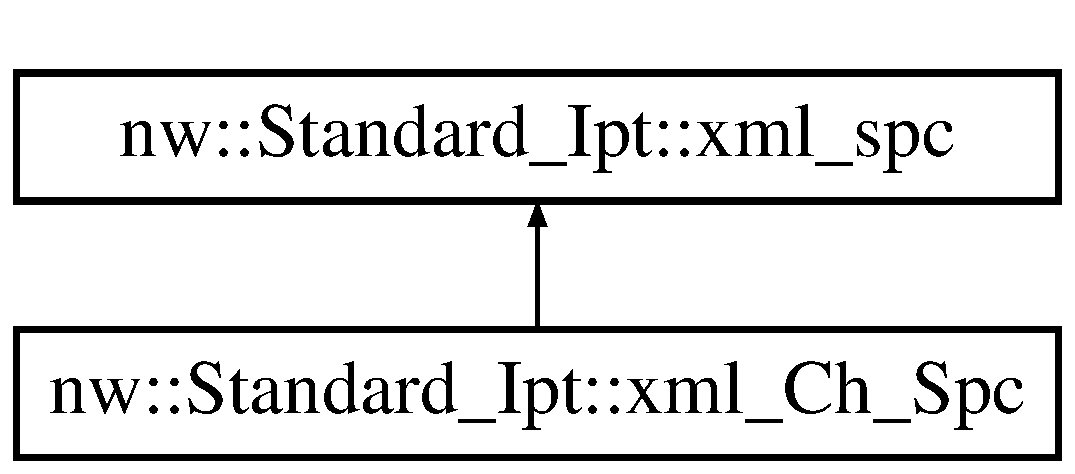
\includegraphics[height=2.000000cm]{d0/d51/structnw_1_1_standard___ipt_1_1xml___ch___spc}
\end{center}
\end{figure}
\subsection*{Public Attributes}
\begin{DoxyCompactItemize}
\item 
long \hyperlink{structnw_1_1_standard___ipt_1_1xml___ch___spc_add361d89d7c6461ba8b6fb75dffa9b82}{xml\+\_\+n\+\_\+subunits}
\item 
long \hyperlink{structnw_1_1_standard___ipt_1_1xml___ch___spc_a7bfa8a0c0cb063b0147a076e4dfcb5f9}{xml\+\_\+n\+\_\+su\+To\+Open}
\end{DoxyCompactItemize}


\subsection{Detailed Description}
Structure with attributes of the \hyperlink{classnw_1_1_channel___spc}{Channel\+\_\+\+Spc} class. 

\subsection{Member Data Documentation}
\hypertarget{structnw_1_1_standard___ipt_1_1xml___ch___spc_add361d89d7c6461ba8b6fb75dffa9b82}{\index{nw\+::\+Standard\+\_\+\+Ipt\+::xml\+\_\+\+Ch\+\_\+\+Spc@{nw\+::\+Standard\+\_\+\+Ipt\+::xml\+\_\+\+Ch\+\_\+\+Spc}!xml\+\_\+n\+\_\+subunits@{xml\+\_\+n\+\_\+subunits}}
\index{xml\+\_\+n\+\_\+subunits@{xml\+\_\+n\+\_\+subunits}!nw\+::\+Standard\+\_\+\+Ipt\+::xml\+\_\+\+Ch\+\_\+\+Spc@{nw\+::\+Standard\+\_\+\+Ipt\+::xml\+\_\+\+Ch\+\_\+\+Spc}}
\subsubsection[{xml\+\_\+n\+\_\+subunits}]{\setlength{\rightskip}{0pt plus 5cm}long nw\+::\+Standard\+\_\+\+Ipt\+::xml\+\_\+\+Ch\+\_\+\+Spc\+::xml\+\_\+n\+\_\+subunits}}\label{structnw_1_1_standard___ipt_1_1xml___ch___spc_add361d89d7c6461ba8b6fb75dffa9b82}
\hypertarget{structnw_1_1_standard___ipt_1_1xml___ch___spc_a7bfa8a0c0cb063b0147a076e4dfcb5f9}{\index{nw\+::\+Standard\+\_\+\+Ipt\+::xml\+\_\+\+Ch\+\_\+\+Spc@{nw\+::\+Standard\+\_\+\+Ipt\+::xml\+\_\+\+Ch\+\_\+\+Spc}!xml\+\_\+n\+\_\+su\+To\+Open@{xml\+\_\+n\+\_\+su\+To\+Open}}
\index{xml\+\_\+n\+\_\+su\+To\+Open@{xml\+\_\+n\+\_\+su\+To\+Open}!nw\+::\+Standard\+\_\+\+Ipt\+::xml\+\_\+\+Ch\+\_\+\+Spc@{nw\+::\+Standard\+\_\+\+Ipt\+::xml\+\_\+\+Ch\+\_\+\+Spc}}
\subsubsection[{xml\+\_\+n\+\_\+su\+To\+Open}]{\setlength{\rightskip}{0pt plus 5cm}long nw\+::\+Standard\+\_\+\+Ipt\+::xml\+\_\+\+Ch\+\_\+\+Spc\+::xml\+\_\+n\+\_\+su\+To\+Open}}\label{structnw_1_1_standard___ipt_1_1xml___ch___spc_a7bfa8a0c0cb063b0147a076e4dfcb5f9}


The documentation for this struct was generated from the following file\+:\begin{DoxyCompactItemize}
\item 
Input/\hyperlink{_standard___ipt_8h}{Standard\+\_\+\+Ipt.\+h}\end{DoxyCompactItemize}

\hypertarget{structnw_1_1_standard___ipt_1_1xml___ch_flux___rct___evt}{\section{nw\+:\+:Standard\+\_\+\+Ipt\+:\+:xml\+\_\+\+Ch\+Flux\+\_\+\+Rct\+\_\+\+Evt Struct Reference}
\label{structnw_1_1_standard___ipt_1_1xml___ch_flux___rct___evt}\index{nw\+::\+Standard\+\_\+\+Ipt\+::xml\+\_\+\+Ch\+Flux\+\_\+\+Rct\+\_\+\+Evt@{nw\+::\+Standard\+\_\+\+Ipt\+::xml\+\_\+\+Ch\+Flux\+\_\+\+Rct\+\_\+\+Evt}}
}


Structure with attributes of the \hyperlink{classnw_1_1_ch_flux___rct___evt}{Ch\+Flux\+\_\+\+Rct\+\_\+\+Evt} class.  


Inheritance diagram for nw\+:\+:Standard\+\_\+\+Ipt\+:\+:xml\+\_\+\+Ch\+Flux\+\_\+\+Rct\+\_\+\+Evt\+:\begin{figure}[H]
\begin{center}
\leavevmode
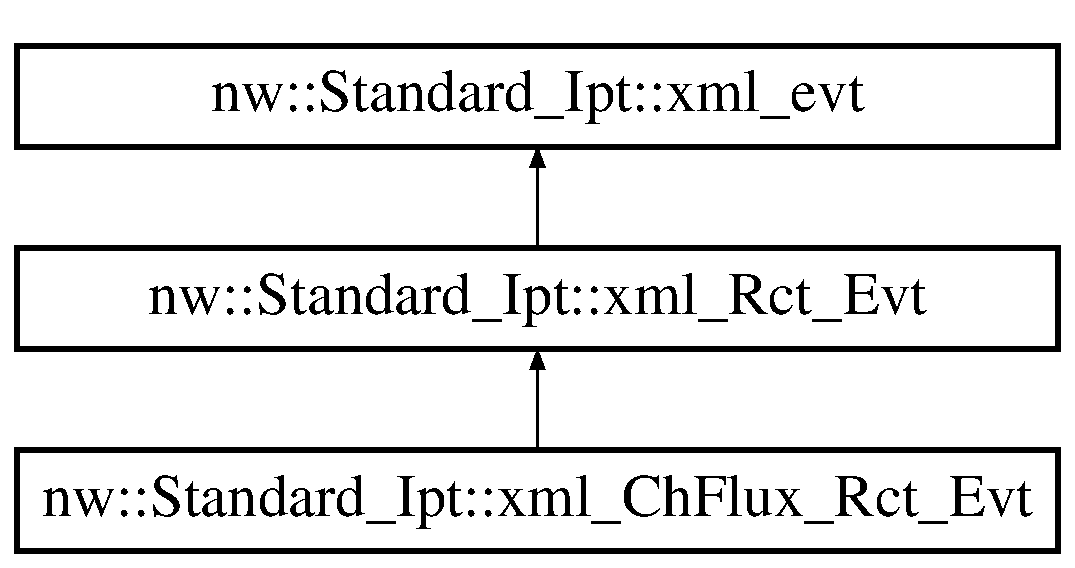
\includegraphics[height=3.000000cm]{d1/d63/structnw_1_1_standard___ipt_1_1xml___ch_flux___rct___evt}
\end{center}
\end{figure}
\subsection*{Public Attributes}
\begin{DoxyCompactItemize}
\item 
long \hyperlink{structnw_1_1_standard___ipt_1_1xml___ch_flux___rct___evt_aa0a4cb6a01e33f4cc0162b1d49a3041c}{xml\+\_\+channel\+\_\+id}
\end{DoxyCompactItemize}


\subsection{Detailed Description}
Structure with attributes of the \hyperlink{classnw_1_1_ch_flux___rct___evt}{Ch\+Flux\+\_\+\+Rct\+\_\+\+Evt} class. 

\subsection{Member Data Documentation}
\hypertarget{structnw_1_1_standard___ipt_1_1xml___ch_flux___rct___evt_aa0a4cb6a01e33f4cc0162b1d49a3041c}{\index{nw\+::\+Standard\+\_\+\+Ipt\+::xml\+\_\+\+Ch\+Flux\+\_\+\+Rct\+\_\+\+Evt@{nw\+::\+Standard\+\_\+\+Ipt\+::xml\+\_\+\+Ch\+Flux\+\_\+\+Rct\+\_\+\+Evt}!xml\+\_\+channel\+\_\+id@{xml\+\_\+channel\+\_\+id}}
\index{xml\+\_\+channel\+\_\+id@{xml\+\_\+channel\+\_\+id}!nw\+::\+Standard\+\_\+\+Ipt\+::xml\+\_\+\+Ch\+Flux\+\_\+\+Rct\+\_\+\+Evt@{nw\+::\+Standard\+\_\+\+Ipt\+::xml\+\_\+\+Ch\+Flux\+\_\+\+Rct\+\_\+\+Evt}}
\subsubsection[{xml\+\_\+channel\+\_\+id}]{\setlength{\rightskip}{0pt plus 5cm}long nw\+::\+Standard\+\_\+\+Ipt\+::xml\+\_\+\+Ch\+Flux\+\_\+\+Rct\+\_\+\+Evt\+::xml\+\_\+channel\+\_\+id}}\label{structnw_1_1_standard___ipt_1_1xml___ch_flux___rct___evt_aa0a4cb6a01e33f4cc0162b1d49a3041c}


The documentation for this struct was generated from the following file\+:\begin{DoxyCompactItemize}
\item 
Input/\hyperlink{_standard___ipt_8h}{Standard\+\_\+\+Ipt.\+h}\end{DoxyCompactItemize}

\hypertarget{structnw_1_1_standard___ipt_1_1xml___dif___evt}{\section{nw\+:\+:Standard\+\_\+\+Ipt\+:\+:xml\+\_\+\+Dif\+\_\+\+Evt Struct Reference}
\label{structnw_1_1_standard___ipt_1_1xml___dif___evt}\index{nw\+::\+Standard\+\_\+\+Ipt\+::xml\+\_\+\+Dif\+\_\+\+Evt@{nw\+::\+Standard\+\_\+\+Ipt\+::xml\+\_\+\+Dif\+\_\+\+Evt}}
}


Structure with attributes of the \hyperlink{classnw_1_1_diffusion___evt}{Diffusion\+\_\+\+Evt} class.  


Inheritance diagram for nw\+:\+:Standard\+\_\+\+Ipt\+:\+:xml\+\_\+\+Dif\+\_\+\+Evt\+:\begin{figure}[H]
\begin{center}
\leavevmode
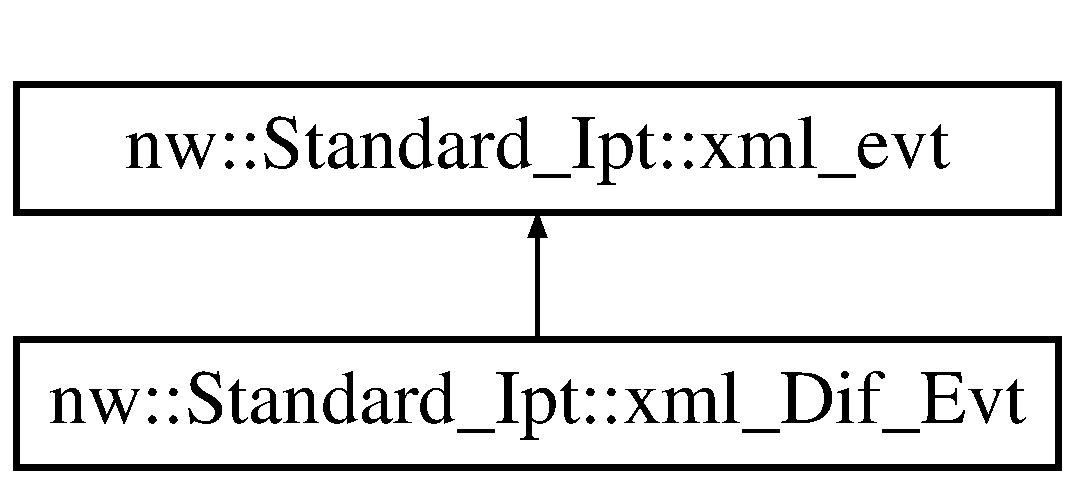
\includegraphics[height=2.000000cm]{de/d1d/structnw_1_1_standard___ipt_1_1xml___dif___evt}
\end{center}
\end{figure}
\subsection*{Public Attributes}
\begin{DoxyCompactItemize}
\item 
long \hyperlink{structnw_1_1_standard___ipt_1_1xml___dif___evt_ac806ec8aa26b8b632163acc327c89d20}{xml\+\_\+diff\+\_\+spc}
\end{DoxyCompactItemize}


\subsection{Detailed Description}
Structure with attributes of the \hyperlink{classnw_1_1_diffusion___evt}{Diffusion\+\_\+\+Evt} class. 

\subsection{Member Data Documentation}
\hypertarget{structnw_1_1_standard___ipt_1_1xml___dif___evt_ac806ec8aa26b8b632163acc327c89d20}{\index{nw\+::\+Standard\+\_\+\+Ipt\+::xml\+\_\+\+Dif\+\_\+\+Evt@{nw\+::\+Standard\+\_\+\+Ipt\+::xml\+\_\+\+Dif\+\_\+\+Evt}!xml\+\_\+diff\+\_\+spc@{xml\+\_\+diff\+\_\+spc}}
\index{xml\+\_\+diff\+\_\+spc@{xml\+\_\+diff\+\_\+spc}!nw\+::\+Standard\+\_\+\+Ipt\+::xml\+\_\+\+Dif\+\_\+\+Evt@{nw\+::\+Standard\+\_\+\+Ipt\+::xml\+\_\+\+Dif\+\_\+\+Evt}}
\subsubsection[{xml\+\_\+diff\+\_\+spc}]{\setlength{\rightskip}{0pt plus 5cm}long nw\+::\+Standard\+\_\+\+Ipt\+::xml\+\_\+\+Dif\+\_\+\+Evt\+::xml\+\_\+diff\+\_\+spc}}\label{structnw_1_1_standard___ipt_1_1xml___dif___evt_ac806ec8aa26b8b632163acc327c89d20}


The documentation for this struct was generated from the following file\+:\begin{DoxyCompactItemize}
\item 
Input/\hyperlink{_standard___ipt_8h}{Standard\+\_\+\+Ipt.\+h}\end{DoxyCompactItemize}

\hypertarget{structnw_1_1_standard___ipt_1_1xml__evt}{\section{nw\+:\+:Standard\+\_\+\+Ipt\+:\+:xml\+\_\+evt Struct Reference}
\label{structnw_1_1_standard___ipt_1_1xml__evt}\index{nw\+::\+Standard\+\_\+\+Ipt\+::xml\+\_\+evt@{nw\+::\+Standard\+\_\+\+Ipt\+::xml\+\_\+evt}}
}


Structure with attributes of the \hyperlink{classnw_1_1___event}{\+\_\+\+Event} class.  


Inheritance diagram for nw\+:\+:Standard\+\_\+\+Ipt\+:\+:xml\+\_\+evt\+:\begin{figure}[H]
\begin{center}
\leavevmode
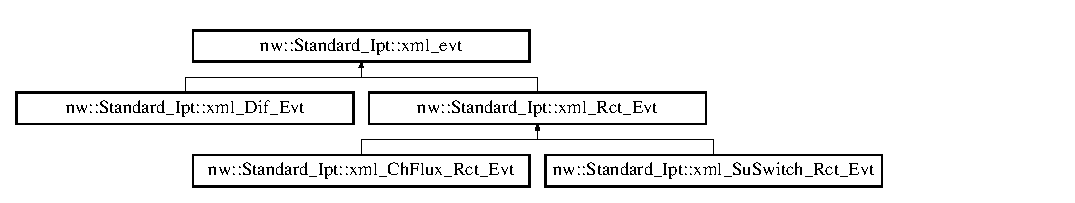
\includegraphics[height=2.276423cm]{db/d3b/structnw_1_1_standard___ipt_1_1xml__evt}
\end{center}
\end{figure}
\subsection*{Public Attributes}
\begin{DoxyCompactItemize}
\item 
long \hyperlink{structnw_1_1_standard___ipt_1_1xml__evt_a7e6815f357b9eae3220c0f4d1f9f6dbd}{xml\+\_\+id}
\item 
string \hyperlink{structnw_1_1_standard___ipt_1_1xml__evt_a2d2a44e9bedde8ef00af81617b057cb9}{xml\+\_\+name}
\item 
double \hyperlink{structnw_1_1_standard___ipt_1_1xml__evt_af8a72fd81f09d6924703af53ad3689ee}{xml\+\_\+k}
\item 
vector$<$ long $>$ \hyperlink{structnw_1_1_standard___ipt_1_1xml__evt_aafc49103df741f710fa1eb6a806f9c24}{xml\+\_\+vxl}
\end{DoxyCompactItemize}


\subsection{Detailed Description}
Structure with attributes of the \hyperlink{classnw_1_1___event}{\+\_\+\+Event} class. 

\subsection{Member Data Documentation}
\hypertarget{structnw_1_1_standard___ipt_1_1xml__evt_a7e6815f357b9eae3220c0f4d1f9f6dbd}{\index{nw\+::\+Standard\+\_\+\+Ipt\+::xml\+\_\+evt@{nw\+::\+Standard\+\_\+\+Ipt\+::xml\+\_\+evt}!xml\+\_\+id@{xml\+\_\+id}}
\index{xml\+\_\+id@{xml\+\_\+id}!nw\+::\+Standard\+\_\+\+Ipt\+::xml\+\_\+evt@{nw\+::\+Standard\+\_\+\+Ipt\+::xml\+\_\+evt}}
\subsubsection[{xml\+\_\+id}]{\setlength{\rightskip}{0pt plus 5cm}long nw\+::\+Standard\+\_\+\+Ipt\+::xml\+\_\+evt\+::xml\+\_\+id}}\label{structnw_1_1_standard___ipt_1_1xml__evt_a7e6815f357b9eae3220c0f4d1f9f6dbd}
\hypertarget{structnw_1_1_standard___ipt_1_1xml__evt_af8a72fd81f09d6924703af53ad3689ee}{\index{nw\+::\+Standard\+\_\+\+Ipt\+::xml\+\_\+evt@{nw\+::\+Standard\+\_\+\+Ipt\+::xml\+\_\+evt}!xml\+\_\+k@{xml\+\_\+k}}
\index{xml\+\_\+k@{xml\+\_\+k}!nw\+::\+Standard\+\_\+\+Ipt\+::xml\+\_\+evt@{nw\+::\+Standard\+\_\+\+Ipt\+::xml\+\_\+evt}}
\subsubsection[{xml\+\_\+k}]{\setlength{\rightskip}{0pt plus 5cm}double nw\+::\+Standard\+\_\+\+Ipt\+::xml\+\_\+evt\+::xml\+\_\+k}}\label{structnw_1_1_standard___ipt_1_1xml__evt_af8a72fd81f09d6924703af53ad3689ee}
\hypertarget{structnw_1_1_standard___ipt_1_1xml__evt_a2d2a44e9bedde8ef00af81617b057cb9}{\index{nw\+::\+Standard\+\_\+\+Ipt\+::xml\+\_\+evt@{nw\+::\+Standard\+\_\+\+Ipt\+::xml\+\_\+evt}!xml\+\_\+name@{xml\+\_\+name}}
\index{xml\+\_\+name@{xml\+\_\+name}!nw\+::\+Standard\+\_\+\+Ipt\+::xml\+\_\+evt@{nw\+::\+Standard\+\_\+\+Ipt\+::xml\+\_\+evt}}
\subsubsection[{xml\+\_\+name}]{\setlength{\rightskip}{0pt plus 5cm}string nw\+::\+Standard\+\_\+\+Ipt\+::xml\+\_\+evt\+::xml\+\_\+name}}\label{structnw_1_1_standard___ipt_1_1xml__evt_a2d2a44e9bedde8ef00af81617b057cb9}
\hypertarget{structnw_1_1_standard___ipt_1_1xml__evt_aafc49103df741f710fa1eb6a806f9c24}{\index{nw\+::\+Standard\+\_\+\+Ipt\+::xml\+\_\+evt@{nw\+::\+Standard\+\_\+\+Ipt\+::xml\+\_\+evt}!xml\+\_\+vxl@{xml\+\_\+vxl}}
\index{xml\+\_\+vxl@{xml\+\_\+vxl}!nw\+::\+Standard\+\_\+\+Ipt\+::xml\+\_\+evt@{nw\+::\+Standard\+\_\+\+Ipt\+::xml\+\_\+evt}}
\subsubsection[{xml\+\_\+vxl}]{\setlength{\rightskip}{0pt plus 5cm}vector$<$long$>$ nw\+::\+Standard\+\_\+\+Ipt\+::xml\+\_\+evt\+::xml\+\_\+vxl}}\label{structnw_1_1_standard___ipt_1_1xml__evt_aafc49103df741f710fa1eb6a806f9c24}


The documentation for this struct was generated from the following file\+:\begin{DoxyCompactItemize}
\item 
Input/\hyperlink{_standard___ipt_8h}{Standard\+\_\+\+Ipt.\+h}\end{DoxyCompactItemize}

\hypertarget{structnw_1_1_standard___ipt_1_1xml__gen__data}{\section{nw\+:\+:Standard\+\_\+\+Ipt\+:\+:xml\+\_\+gen\+\_\+data Struct Reference}
\label{structnw_1_1_standard___ipt_1_1xml__gen__data}\index{nw\+::\+Standard\+\_\+\+Ipt\+::xml\+\_\+gen\+\_\+data@{nw\+::\+Standard\+\_\+\+Ipt\+::xml\+\_\+gen\+\_\+data}}
}


Structure with attributes representing general data necessary for a system.  


\subsection*{Public Attributes}
\begin{DoxyCompactItemize}
\item 
string \hyperlink{structnw_1_1_standard___ipt_1_1xml__gen__data_a68513493e94011fcaacbd9049808017d}{xml\+\_\+simulation\+\_\+type}
\item 
string \hyperlink{structnw_1_1_standard___ipt_1_1xml__gen__data_adc59bb5516c7b0c34463e5c1b446bf6a}{xml\+\_\+border\+\_\+condition}
\item 
long \hyperlink{structnw_1_1_standard___ipt_1_1xml__gen__data_a942847ef13274b631a767f65d0a5ff3c}{xml\+\_\+output\+\_\+mode}
\item 
double \hyperlink{structnw_1_1_standard___ipt_1_1xml__gen__data_a757ebd2e9fd83412731faf6bb2059dd5}{xml\+\_\+max\+\_\+sim\+\_\+steps}
\item 
double \hyperlink{structnw_1_1_standard___ipt_1_1xml__gen__data_a2b0da231be5d3a1e159730a63008950b}{xml\+\_\+max\+\_\+sim\+\_\+time}
\item 
double \hyperlink{structnw_1_1_standard___ipt_1_1xml__gen__data_ab5ae087bdf7edb268aca5b736c7cde27}{xml\+\_\+sample\+\_\+rate}
\item 
double \hyperlink{structnw_1_1_standard___ipt_1_1xml__gen__data_aa778758339d3c6beb926e4df3341e5a2}{xml\+\_\+box\+\_\+lenght}
\item 
vector$<$ long $>$ \hyperlink{structnw_1_1_standard___ipt_1_1xml__gen__data_a9bbeaad11219c26143f2c45915caeabc}{xml\+\_\+output\+\_\+\+Spc}
\item 
vector$<$ long $>$ \hyperlink{structnw_1_1_standard___ipt_1_1xml__gen__data_a6a41a161744c03226daa444501a2df6c}{xml\+\_\+output\+\_\+\+Vxl}
\item 
vector$<$ \hyperlink{structnw_1_1_standard___ipt_1_1xml___rct___evt}{xml\+\_\+\+Rct\+\_\+\+Evt} $\ast$ $>$ \hyperlink{structnw_1_1_standard___ipt_1_1xml__gen__data_abc4e7ae5a154343c1d3d25917bd58a5f}{xml\+\_\+rct\+\_\+evt\+\_\+list}
\item 
vector$<$ \hyperlink{structnw_1_1_standard___ipt_1_1xml___dif___evt}{xml\+\_\+\+Dif\+\_\+\+Evt} $\ast$ $>$ \hyperlink{structnw_1_1_standard___ipt_1_1xml__gen__data_a115f67778a3d29d716303c194354d2f7}{xml\+\_\+dif\+\_\+evt\+\_\+list}
\item 
vector$<$ \hyperlink{structnw_1_1_standard___ipt_1_1xml___su_switch___rct___evt}{xml\+\_\+\+Su\+Switch\+\_\+\+Rct\+\_\+\+Evt} $\ast$ $>$ \hyperlink{structnw_1_1_standard___ipt_1_1xml__gen__data_a4da34a5918c4e045ed5021da6fdbc6bf}{xml\+\_\+su\+Switch\+\_\+rct\+\_\+evt\+\_\+list}
\item 
vector$<$ \hyperlink{structnw_1_1_standard___ipt_1_1xml___ch_flux___rct___evt}{xml\+\_\+\+Ch\+Flux\+\_\+\+Rct\+\_\+\+Evt} $\ast$ $>$ \hyperlink{structnw_1_1_standard___ipt_1_1xml__gen__data_ae0479559e90fe38932ac604852a1541f}{xml\+\_\+ch\+Flux\+\_\+rct\+\_\+evt\+\_\+list}
\item 
vector$<$ \hyperlink{structnw_1_1_standard___ipt_1_1xml__vxl}{xml\+\_\+vxl} $\ast$ $>$ \hyperlink{structnw_1_1_standard___ipt_1_1xml__gen__data_af091596661fc87ef8c7f28317555c6af}{xml\+\_\+vxl\+\_\+list}
\item 
vector$<$ \hyperlink{structnw_1_1_standard___ipt_1_1xml__spc}{xml\+\_\+spc} $\ast$ $>$ \hyperlink{structnw_1_1_standard___ipt_1_1xml__gen__data_a70786e61ea513972d7c50982e101726c}{xml\+\_\+spc\+\_\+list}
\item 
vector$<$ \hyperlink{structnw_1_1_standard___ipt_1_1xml___ch___spc}{xml\+\_\+\+Ch\+\_\+\+Spc} $\ast$ $>$ \hyperlink{structnw_1_1_standard___ipt_1_1xml__gen__data_ab46c43b495fd3d278ffeabe88261d36e}{xml\+\_\+ch\+\_\+spc\+\_\+list}
\end{DoxyCompactItemize}


\subsection{Detailed Description}
Structure with attributes representing general data necessary for a system. 

\subsection{Member Data Documentation}
\hypertarget{structnw_1_1_standard___ipt_1_1xml__gen__data_adc59bb5516c7b0c34463e5c1b446bf6a}{\index{nw\+::\+Standard\+\_\+\+Ipt\+::xml\+\_\+gen\+\_\+data@{nw\+::\+Standard\+\_\+\+Ipt\+::xml\+\_\+gen\+\_\+data}!xml\+\_\+border\+\_\+condition@{xml\+\_\+border\+\_\+condition}}
\index{xml\+\_\+border\+\_\+condition@{xml\+\_\+border\+\_\+condition}!nw\+::\+Standard\+\_\+\+Ipt\+::xml\+\_\+gen\+\_\+data@{nw\+::\+Standard\+\_\+\+Ipt\+::xml\+\_\+gen\+\_\+data}}
\subsubsection[{xml\+\_\+border\+\_\+condition}]{\setlength{\rightskip}{0pt plus 5cm}string nw\+::\+Standard\+\_\+\+Ipt\+::xml\+\_\+gen\+\_\+data\+::xml\+\_\+border\+\_\+condition}}\label{structnw_1_1_standard___ipt_1_1xml__gen__data_adc59bb5516c7b0c34463e5c1b446bf6a}
\hypertarget{structnw_1_1_standard___ipt_1_1xml__gen__data_aa778758339d3c6beb926e4df3341e5a2}{\index{nw\+::\+Standard\+\_\+\+Ipt\+::xml\+\_\+gen\+\_\+data@{nw\+::\+Standard\+\_\+\+Ipt\+::xml\+\_\+gen\+\_\+data}!xml\+\_\+box\+\_\+lenght@{xml\+\_\+box\+\_\+lenght}}
\index{xml\+\_\+box\+\_\+lenght@{xml\+\_\+box\+\_\+lenght}!nw\+::\+Standard\+\_\+\+Ipt\+::xml\+\_\+gen\+\_\+data@{nw\+::\+Standard\+\_\+\+Ipt\+::xml\+\_\+gen\+\_\+data}}
\subsubsection[{xml\+\_\+box\+\_\+lenght}]{\setlength{\rightskip}{0pt plus 5cm}double nw\+::\+Standard\+\_\+\+Ipt\+::xml\+\_\+gen\+\_\+data\+::xml\+\_\+box\+\_\+lenght}}\label{structnw_1_1_standard___ipt_1_1xml__gen__data_aa778758339d3c6beb926e4df3341e5a2}
\hypertarget{structnw_1_1_standard___ipt_1_1xml__gen__data_ab46c43b495fd3d278ffeabe88261d36e}{\index{nw\+::\+Standard\+\_\+\+Ipt\+::xml\+\_\+gen\+\_\+data@{nw\+::\+Standard\+\_\+\+Ipt\+::xml\+\_\+gen\+\_\+data}!xml\+\_\+ch\+\_\+spc\+\_\+list@{xml\+\_\+ch\+\_\+spc\+\_\+list}}
\index{xml\+\_\+ch\+\_\+spc\+\_\+list@{xml\+\_\+ch\+\_\+spc\+\_\+list}!nw\+::\+Standard\+\_\+\+Ipt\+::xml\+\_\+gen\+\_\+data@{nw\+::\+Standard\+\_\+\+Ipt\+::xml\+\_\+gen\+\_\+data}}
\subsubsection[{xml\+\_\+ch\+\_\+spc\+\_\+list}]{\setlength{\rightskip}{0pt plus 5cm}vector$<${\bf xml\+\_\+\+Ch\+\_\+\+Spc}$\ast$$>$ nw\+::\+Standard\+\_\+\+Ipt\+::xml\+\_\+gen\+\_\+data\+::xml\+\_\+ch\+\_\+spc\+\_\+list}}\label{structnw_1_1_standard___ipt_1_1xml__gen__data_ab46c43b495fd3d278ffeabe88261d36e}
\hypertarget{structnw_1_1_standard___ipt_1_1xml__gen__data_ae0479559e90fe38932ac604852a1541f}{\index{nw\+::\+Standard\+\_\+\+Ipt\+::xml\+\_\+gen\+\_\+data@{nw\+::\+Standard\+\_\+\+Ipt\+::xml\+\_\+gen\+\_\+data}!xml\+\_\+ch\+Flux\+\_\+rct\+\_\+evt\+\_\+list@{xml\+\_\+ch\+Flux\+\_\+rct\+\_\+evt\+\_\+list}}
\index{xml\+\_\+ch\+Flux\+\_\+rct\+\_\+evt\+\_\+list@{xml\+\_\+ch\+Flux\+\_\+rct\+\_\+evt\+\_\+list}!nw\+::\+Standard\+\_\+\+Ipt\+::xml\+\_\+gen\+\_\+data@{nw\+::\+Standard\+\_\+\+Ipt\+::xml\+\_\+gen\+\_\+data}}
\subsubsection[{xml\+\_\+ch\+Flux\+\_\+rct\+\_\+evt\+\_\+list}]{\setlength{\rightskip}{0pt plus 5cm}vector$<${\bf xml\+\_\+\+Ch\+Flux\+\_\+\+Rct\+\_\+\+Evt}$\ast$$>$ nw\+::\+Standard\+\_\+\+Ipt\+::xml\+\_\+gen\+\_\+data\+::xml\+\_\+ch\+Flux\+\_\+rct\+\_\+evt\+\_\+list}}\label{structnw_1_1_standard___ipt_1_1xml__gen__data_ae0479559e90fe38932ac604852a1541f}
\hypertarget{structnw_1_1_standard___ipt_1_1xml__gen__data_a115f67778a3d29d716303c194354d2f7}{\index{nw\+::\+Standard\+\_\+\+Ipt\+::xml\+\_\+gen\+\_\+data@{nw\+::\+Standard\+\_\+\+Ipt\+::xml\+\_\+gen\+\_\+data}!xml\+\_\+dif\+\_\+evt\+\_\+list@{xml\+\_\+dif\+\_\+evt\+\_\+list}}
\index{xml\+\_\+dif\+\_\+evt\+\_\+list@{xml\+\_\+dif\+\_\+evt\+\_\+list}!nw\+::\+Standard\+\_\+\+Ipt\+::xml\+\_\+gen\+\_\+data@{nw\+::\+Standard\+\_\+\+Ipt\+::xml\+\_\+gen\+\_\+data}}
\subsubsection[{xml\+\_\+dif\+\_\+evt\+\_\+list}]{\setlength{\rightskip}{0pt plus 5cm}vector$<${\bf xml\+\_\+\+Dif\+\_\+\+Evt}$\ast$$>$ nw\+::\+Standard\+\_\+\+Ipt\+::xml\+\_\+gen\+\_\+data\+::xml\+\_\+dif\+\_\+evt\+\_\+list}}\label{structnw_1_1_standard___ipt_1_1xml__gen__data_a115f67778a3d29d716303c194354d2f7}
\hypertarget{structnw_1_1_standard___ipt_1_1xml__gen__data_a757ebd2e9fd83412731faf6bb2059dd5}{\index{nw\+::\+Standard\+\_\+\+Ipt\+::xml\+\_\+gen\+\_\+data@{nw\+::\+Standard\+\_\+\+Ipt\+::xml\+\_\+gen\+\_\+data}!xml\+\_\+max\+\_\+sim\+\_\+steps@{xml\+\_\+max\+\_\+sim\+\_\+steps}}
\index{xml\+\_\+max\+\_\+sim\+\_\+steps@{xml\+\_\+max\+\_\+sim\+\_\+steps}!nw\+::\+Standard\+\_\+\+Ipt\+::xml\+\_\+gen\+\_\+data@{nw\+::\+Standard\+\_\+\+Ipt\+::xml\+\_\+gen\+\_\+data}}
\subsubsection[{xml\+\_\+max\+\_\+sim\+\_\+steps}]{\setlength{\rightskip}{0pt plus 5cm}double nw\+::\+Standard\+\_\+\+Ipt\+::xml\+\_\+gen\+\_\+data\+::xml\+\_\+max\+\_\+sim\+\_\+steps}}\label{structnw_1_1_standard___ipt_1_1xml__gen__data_a757ebd2e9fd83412731faf6bb2059dd5}
\hypertarget{structnw_1_1_standard___ipt_1_1xml__gen__data_a2b0da231be5d3a1e159730a63008950b}{\index{nw\+::\+Standard\+\_\+\+Ipt\+::xml\+\_\+gen\+\_\+data@{nw\+::\+Standard\+\_\+\+Ipt\+::xml\+\_\+gen\+\_\+data}!xml\+\_\+max\+\_\+sim\+\_\+time@{xml\+\_\+max\+\_\+sim\+\_\+time}}
\index{xml\+\_\+max\+\_\+sim\+\_\+time@{xml\+\_\+max\+\_\+sim\+\_\+time}!nw\+::\+Standard\+\_\+\+Ipt\+::xml\+\_\+gen\+\_\+data@{nw\+::\+Standard\+\_\+\+Ipt\+::xml\+\_\+gen\+\_\+data}}
\subsubsection[{xml\+\_\+max\+\_\+sim\+\_\+time}]{\setlength{\rightskip}{0pt plus 5cm}double nw\+::\+Standard\+\_\+\+Ipt\+::xml\+\_\+gen\+\_\+data\+::xml\+\_\+max\+\_\+sim\+\_\+time}}\label{structnw_1_1_standard___ipt_1_1xml__gen__data_a2b0da231be5d3a1e159730a63008950b}
\hypertarget{structnw_1_1_standard___ipt_1_1xml__gen__data_a942847ef13274b631a767f65d0a5ff3c}{\index{nw\+::\+Standard\+\_\+\+Ipt\+::xml\+\_\+gen\+\_\+data@{nw\+::\+Standard\+\_\+\+Ipt\+::xml\+\_\+gen\+\_\+data}!xml\+\_\+output\+\_\+mode@{xml\+\_\+output\+\_\+mode}}
\index{xml\+\_\+output\+\_\+mode@{xml\+\_\+output\+\_\+mode}!nw\+::\+Standard\+\_\+\+Ipt\+::xml\+\_\+gen\+\_\+data@{nw\+::\+Standard\+\_\+\+Ipt\+::xml\+\_\+gen\+\_\+data}}
\subsubsection[{xml\+\_\+output\+\_\+mode}]{\setlength{\rightskip}{0pt plus 5cm}long nw\+::\+Standard\+\_\+\+Ipt\+::xml\+\_\+gen\+\_\+data\+::xml\+\_\+output\+\_\+mode}}\label{structnw_1_1_standard___ipt_1_1xml__gen__data_a942847ef13274b631a767f65d0a5ff3c}
\hypertarget{structnw_1_1_standard___ipt_1_1xml__gen__data_a9bbeaad11219c26143f2c45915caeabc}{\index{nw\+::\+Standard\+\_\+\+Ipt\+::xml\+\_\+gen\+\_\+data@{nw\+::\+Standard\+\_\+\+Ipt\+::xml\+\_\+gen\+\_\+data}!xml\+\_\+output\+\_\+\+Spc@{xml\+\_\+output\+\_\+\+Spc}}
\index{xml\+\_\+output\+\_\+\+Spc@{xml\+\_\+output\+\_\+\+Spc}!nw\+::\+Standard\+\_\+\+Ipt\+::xml\+\_\+gen\+\_\+data@{nw\+::\+Standard\+\_\+\+Ipt\+::xml\+\_\+gen\+\_\+data}}
\subsubsection[{xml\+\_\+output\+\_\+\+Spc}]{\setlength{\rightskip}{0pt plus 5cm}vector$<$long$>$ nw\+::\+Standard\+\_\+\+Ipt\+::xml\+\_\+gen\+\_\+data\+::xml\+\_\+output\+\_\+\+Spc}}\label{structnw_1_1_standard___ipt_1_1xml__gen__data_a9bbeaad11219c26143f2c45915caeabc}
\hypertarget{structnw_1_1_standard___ipt_1_1xml__gen__data_a6a41a161744c03226daa444501a2df6c}{\index{nw\+::\+Standard\+\_\+\+Ipt\+::xml\+\_\+gen\+\_\+data@{nw\+::\+Standard\+\_\+\+Ipt\+::xml\+\_\+gen\+\_\+data}!xml\+\_\+output\+\_\+\+Vxl@{xml\+\_\+output\+\_\+\+Vxl}}
\index{xml\+\_\+output\+\_\+\+Vxl@{xml\+\_\+output\+\_\+\+Vxl}!nw\+::\+Standard\+\_\+\+Ipt\+::xml\+\_\+gen\+\_\+data@{nw\+::\+Standard\+\_\+\+Ipt\+::xml\+\_\+gen\+\_\+data}}
\subsubsection[{xml\+\_\+output\+\_\+\+Vxl}]{\setlength{\rightskip}{0pt plus 5cm}vector$<$long$>$ nw\+::\+Standard\+\_\+\+Ipt\+::xml\+\_\+gen\+\_\+data\+::xml\+\_\+output\+\_\+\+Vxl}}\label{structnw_1_1_standard___ipt_1_1xml__gen__data_a6a41a161744c03226daa444501a2df6c}
\hypertarget{structnw_1_1_standard___ipt_1_1xml__gen__data_abc4e7ae5a154343c1d3d25917bd58a5f}{\index{nw\+::\+Standard\+\_\+\+Ipt\+::xml\+\_\+gen\+\_\+data@{nw\+::\+Standard\+\_\+\+Ipt\+::xml\+\_\+gen\+\_\+data}!xml\+\_\+rct\+\_\+evt\+\_\+list@{xml\+\_\+rct\+\_\+evt\+\_\+list}}
\index{xml\+\_\+rct\+\_\+evt\+\_\+list@{xml\+\_\+rct\+\_\+evt\+\_\+list}!nw\+::\+Standard\+\_\+\+Ipt\+::xml\+\_\+gen\+\_\+data@{nw\+::\+Standard\+\_\+\+Ipt\+::xml\+\_\+gen\+\_\+data}}
\subsubsection[{xml\+\_\+rct\+\_\+evt\+\_\+list}]{\setlength{\rightskip}{0pt plus 5cm}vector$<${\bf xml\+\_\+\+Rct\+\_\+\+Evt}$\ast$$>$ nw\+::\+Standard\+\_\+\+Ipt\+::xml\+\_\+gen\+\_\+data\+::xml\+\_\+rct\+\_\+evt\+\_\+list}}\label{structnw_1_1_standard___ipt_1_1xml__gen__data_abc4e7ae5a154343c1d3d25917bd58a5f}
\hypertarget{structnw_1_1_standard___ipt_1_1xml__gen__data_ab5ae087bdf7edb268aca5b736c7cde27}{\index{nw\+::\+Standard\+\_\+\+Ipt\+::xml\+\_\+gen\+\_\+data@{nw\+::\+Standard\+\_\+\+Ipt\+::xml\+\_\+gen\+\_\+data}!xml\+\_\+sample\+\_\+rate@{xml\+\_\+sample\+\_\+rate}}
\index{xml\+\_\+sample\+\_\+rate@{xml\+\_\+sample\+\_\+rate}!nw\+::\+Standard\+\_\+\+Ipt\+::xml\+\_\+gen\+\_\+data@{nw\+::\+Standard\+\_\+\+Ipt\+::xml\+\_\+gen\+\_\+data}}
\subsubsection[{xml\+\_\+sample\+\_\+rate}]{\setlength{\rightskip}{0pt plus 5cm}double nw\+::\+Standard\+\_\+\+Ipt\+::xml\+\_\+gen\+\_\+data\+::xml\+\_\+sample\+\_\+rate}}\label{structnw_1_1_standard___ipt_1_1xml__gen__data_ab5ae087bdf7edb268aca5b736c7cde27}
\hypertarget{structnw_1_1_standard___ipt_1_1xml__gen__data_a68513493e94011fcaacbd9049808017d}{\index{nw\+::\+Standard\+\_\+\+Ipt\+::xml\+\_\+gen\+\_\+data@{nw\+::\+Standard\+\_\+\+Ipt\+::xml\+\_\+gen\+\_\+data}!xml\+\_\+simulation\+\_\+type@{xml\+\_\+simulation\+\_\+type}}
\index{xml\+\_\+simulation\+\_\+type@{xml\+\_\+simulation\+\_\+type}!nw\+::\+Standard\+\_\+\+Ipt\+::xml\+\_\+gen\+\_\+data@{nw\+::\+Standard\+\_\+\+Ipt\+::xml\+\_\+gen\+\_\+data}}
\subsubsection[{xml\+\_\+simulation\+\_\+type}]{\setlength{\rightskip}{0pt plus 5cm}string nw\+::\+Standard\+\_\+\+Ipt\+::xml\+\_\+gen\+\_\+data\+::xml\+\_\+simulation\+\_\+type}}\label{structnw_1_1_standard___ipt_1_1xml__gen__data_a68513493e94011fcaacbd9049808017d}
\hypertarget{structnw_1_1_standard___ipt_1_1xml__gen__data_a70786e61ea513972d7c50982e101726c}{\index{nw\+::\+Standard\+\_\+\+Ipt\+::xml\+\_\+gen\+\_\+data@{nw\+::\+Standard\+\_\+\+Ipt\+::xml\+\_\+gen\+\_\+data}!xml\+\_\+spc\+\_\+list@{xml\+\_\+spc\+\_\+list}}
\index{xml\+\_\+spc\+\_\+list@{xml\+\_\+spc\+\_\+list}!nw\+::\+Standard\+\_\+\+Ipt\+::xml\+\_\+gen\+\_\+data@{nw\+::\+Standard\+\_\+\+Ipt\+::xml\+\_\+gen\+\_\+data}}
\subsubsection[{xml\+\_\+spc\+\_\+list}]{\setlength{\rightskip}{0pt plus 5cm}vector$<${\bf xml\+\_\+spc}$\ast$$>$ nw\+::\+Standard\+\_\+\+Ipt\+::xml\+\_\+gen\+\_\+data\+::xml\+\_\+spc\+\_\+list}}\label{structnw_1_1_standard___ipt_1_1xml__gen__data_a70786e61ea513972d7c50982e101726c}
\hypertarget{structnw_1_1_standard___ipt_1_1xml__gen__data_a4da34a5918c4e045ed5021da6fdbc6bf}{\index{nw\+::\+Standard\+\_\+\+Ipt\+::xml\+\_\+gen\+\_\+data@{nw\+::\+Standard\+\_\+\+Ipt\+::xml\+\_\+gen\+\_\+data}!xml\+\_\+su\+Switch\+\_\+rct\+\_\+evt\+\_\+list@{xml\+\_\+su\+Switch\+\_\+rct\+\_\+evt\+\_\+list}}
\index{xml\+\_\+su\+Switch\+\_\+rct\+\_\+evt\+\_\+list@{xml\+\_\+su\+Switch\+\_\+rct\+\_\+evt\+\_\+list}!nw\+::\+Standard\+\_\+\+Ipt\+::xml\+\_\+gen\+\_\+data@{nw\+::\+Standard\+\_\+\+Ipt\+::xml\+\_\+gen\+\_\+data}}
\subsubsection[{xml\+\_\+su\+Switch\+\_\+rct\+\_\+evt\+\_\+list}]{\setlength{\rightskip}{0pt plus 5cm}vector$<${\bf xml\+\_\+\+Su\+Switch\+\_\+\+Rct\+\_\+\+Evt}$\ast$$>$ nw\+::\+Standard\+\_\+\+Ipt\+::xml\+\_\+gen\+\_\+data\+::xml\+\_\+su\+Switch\+\_\+rct\+\_\+evt\+\_\+list}}\label{structnw_1_1_standard___ipt_1_1xml__gen__data_a4da34a5918c4e045ed5021da6fdbc6bf}
\hypertarget{structnw_1_1_standard___ipt_1_1xml__gen__data_af091596661fc87ef8c7f28317555c6af}{\index{nw\+::\+Standard\+\_\+\+Ipt\+::xml\+\_\+gen\+\_\+data@{nw\+::\+Standard\+\_\+\+Ipt\+::xml\+\_\+gen\+\_\+data}!xml\+\_\+vxl\+\_\+list@{xml\+\_\+vxl\+\_\+list}}
\index{xml\+\_\+vxl\+\_\+list@{xml\+\_\+vxl\+\_\+list}!nw\+::\+Standard\+\_\+\+Ipt\+::xml\+\_\+gen\+\_\+data@{nw\+::\+Standard\+\_\+\+Ipt\+::xml\+\_\+gen\+\_\+data}}
\subsubsection[{xml\+\_\+vxl\+\_\+list}]{\setlength{\rightskip}{0pt plus 5cm}vector$<${\bf xml\+\_\+vxl}$\ast$$>$ nw\+::\+Standard\+\_\+\+Ipt\+::xml\+\_\+gen\+\_\+data\+::xml\+\_\+vxl\+\_\+list}}\label{structnw_1_1_standard___ipt_1_1xml__gen__data_af091596661fc87ef8c7f28317555c6af}


The documentation for this struct was generated from the following file\+:\begin{DoxyCompactItemize}
\item 
Input/\hyperlink{_standard___ipt_8h}{Standard\+\_\+\+Ipt.\+h}\end{DoxyCompactItemize}

\hypertarget{structnw_1_1_standard___ipt_1_1xml___rct___evt}{\section{nw\+:\+:Standard\+\_\+\+Ipt\+:\+:xml\+\_\+\+Rct\+\_\+\+Evt Struct Reference}
\label{structnw_1_1_standard___ipt_1_1xml___rct___evt}\index{nw\+::\+Standard\+\_\+\+Ipt\+::xml\+\_\+\+Rct\+\_\+\+Evt@{nw\+::\+Standard\+\_\+\+Ipt\+::xml\+\_\+\+Rct\+\_\+\+Evt}}
}


Structure with attributes of the \hyperlink{classnw_1_1_reaction___evt}{Reaction\+\_\+\+Evt} class.  


Inheritance diagram for nw\+:\+:Standard\+\_\+\+Ipt\+:\+:xml\+\_\+\+Rct\+\_\+\+Evt\+:\begin{figure}[H]
\begin{center}
\leavevmode
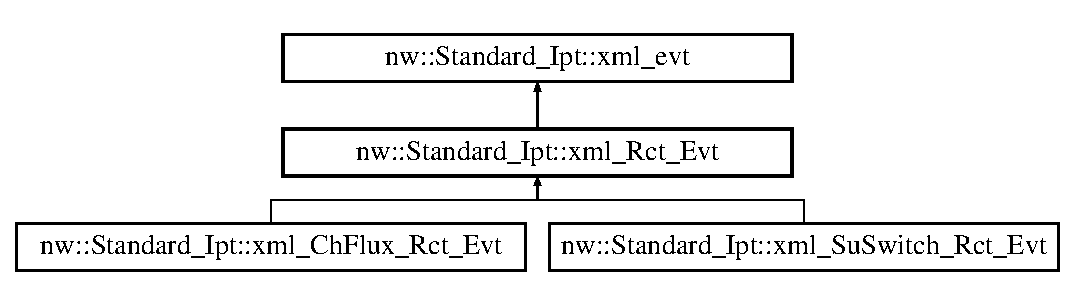
\includegraphics[height=3.000000cm]{d4/d3d/structnw_1_1_standard___ipt_1_1xml___rct___evt}
\end{center}
\end{figure}
\subsection*{Public Attributes}
\begin{DoxyCompactItemize}
\item 
vector$<$ long $>$ \hyperlink{structnw_1_1_standard___ipt_1_1xml___rct___evt_a7bee357e0554eb7a6bba9fff6624e5ad}{xml\+\_\+educts}
\item 
vector$<$ long $>$ \hyperlink{structnw_1_1_standard___ipt_1_1xml___rct___evt_a2c8054ac2dbef43234927778f80ae4e6}{xml\+\_\+products}
\end{DoxyCompactItemize}


\subsection{Detailed Description}
Structure with attributes of the \hyperlink{classnw_1_1_reaction___evt}{Reaction\+\_\+\+Evt} class. 

\subsection{Member Data Documentation}
\hypertarget{structnw_1_1_standard___ipt_1_1xml___rct___evt_a7bee357e0554eb7a6bba9fff6624e5ad}{\index{nw\+::\+Standard\+\_\+\+Ipt\+::xml\+\_\+\+Rct\+\_\+\+Evt@{nw\+::\+Standard\+\_\+\+Ipt\+::xml\+\_\+\+Rct\+\_\+\+Evt}!xml\+\_\+educts@{xml\+\_\+educts}}
\index{xml\+\_\+educts@{xml\+\_\+educts}!nw\+::\+Standard\+\_\+\+Ipt\+::xml\+\_\+\+Rct\+\_\+\+Evt@{nw\+::\+Standard\+\_\+\+Ipt\+::xml\+\_\+\+Rct\+\_\+\+Evt}}
\subsubsection[{xml\+\_\+educts}]{\setlength{\rightskip}{0pt plus 5cm}vector$<$long$>$ nw\+::\+Standard\+\_\+\+Ipt\+::xml\+\_\+\+Rct\+\_\+\+Evt\+::xml\+\_\+educts}}\label{structnw_1_1_standard___ipt_1_1xml___rct___evt_a7bee357e0554eb7a6bba9fff6624e5ad}
\hypertarget{structnw_1_1_standard___ipt_1_1xml___rct___evt_a2c8054ac2dbef43234927778f80ae4e6}{\index{nw\+::\+Standard\+\_\+\+Ipt\+::xml\+\_\+\+Rct\+\_\+\+Evt@{nw\+::\+Standard\+\_\+\+Ipt\+::xml\+\_\+\+Rct\+\_\+\+Evt}!xml\+\_\+products@{xml\+\_\+products}}
\index{xml\+\_\+products@{xml\+\_\+products}!nw\+::\+Standard\+\_\+\+Ipt\+::xml\+\_\+\+Rct\+\_\+\+Evt@{nw\+::\+Standard\+\_\+\+Ipt\+::xml\+\_\+\+Rct\+\_\+\+Evt}}
\subsubsection[{xml\+\_\+products}]{\setlength{\rightskip}{0pt plus 5cm}vector$<$long$>$ nw\+::\+Standard\+\_\+\+Ipt\+::xml\+\_\+\+Rct\+\_\+\+Evt\+::xml\+\_\+products}}\label{structnw_1_1_standard___ipt_1_1xml___rct___evt_a2c8054ac2dbef43234927778f80ae4e6}


The documentation for this struct was generated from the following file\+:\begin{DoxyCompactItemize}
\item 
Input/\hyperlink{_standard___ipt_8h}{Standard\+\_\+\+Ipt.\+h}\end{DoxyCompactItemize}

\hypertarget{structnw_1_1_standard___ipt_1_1xml__spc}{\section{nw\+:\+:Standard\+\_\+\+Ipt\+:\+:xml\+\_\+spc Struct Reference}
\label{structnw_1_1_standard___ipt_1_1xml__spc}\index{nw\+::\+Standard\+\_\+\+Ipt\+::xml\+\_\+spc@{nw\+::\+Standard\+\_\+\+Ipt\+::xml\+\_\+spc}}
}


Structure with attributes of the \hyperlink{classnw_1_1___species}{\+\_\+\+Species} class.  


Inheritance diagram for nw\+:\+:Standard\+\_\+\+Ipt\+:\+:xml\+\_\+spc\+:\begin{figure}[H]
\begin{center}
\leavevmode
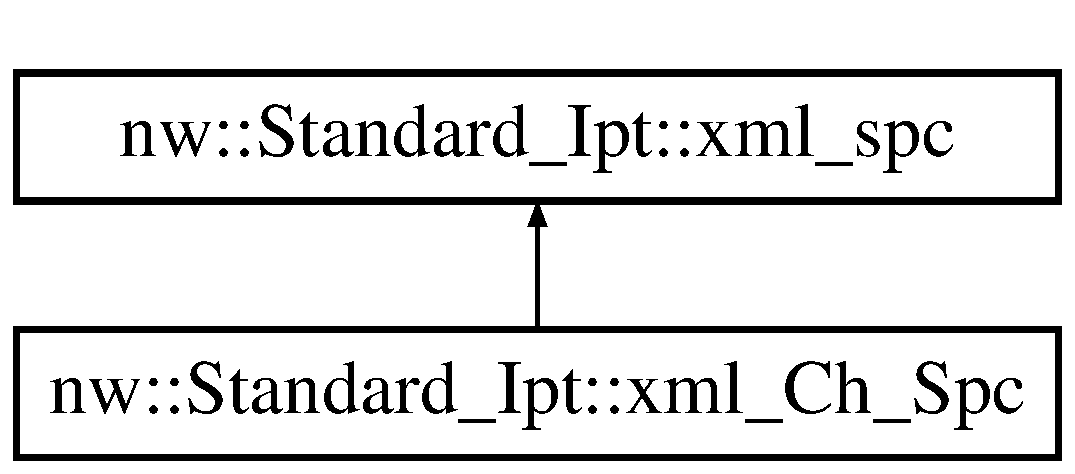
\includegraphics[height=2.000000cm]{df/d8c/structnw_1_1_standard___ipt_1_1xml__spc}
\end{center}
\end{figure}
\subsection*{Public Attributes}
\begin{DoxyCompactItemize}
\item 
long \hyperlink{structnw_1_1_standard___ipt_1_1xml__spc_a2928ff822d6fd953e125ec3d8dd741d9}{xml\+\_\+id}
\item 
string \hyperlink{structnw_1_1_standard___ipt_1_1xml__spc_a2b1626e44822991931ca0dfd7257c95f}{xml\+\_\+name}
\item 
double \hyperlink{structnw_1_1_standard___ipt_1_1xml__spc_a1ae4e41f07db5f76deb50901ee12dc2e}{xml\+\_\+init\+\_\+conc}
\end{DoxyCompactItemize}


\subsection{Detailed Description}
Structure with attributes of the \hyperlink{classnw_1_1___species}{\+\_\+\+Species} class. 

\subsection{Member Data Documentation}
\hypertarget{structnw_1_1_standard___ipt_1_1xml__spc_a2928ff822d6fd953e125ec3d8dd741d9}{\index{nw\+::\+Standard\+\_\+\+Ipt\+::xml\+\_\+spc@{nw\+::\+Standard\+\_\+\+Ipt\+::xml\+\_\+spc}!xml\+\_\+id@{xml\+\_\+id}}
\index{xml\+\_\+id@{xml\+\_\+id}!nw\+::\+Standard\+\_\+\+Ipt\+::xml\+\_\+spc@{nw\+::\+Standard\+\_\+\+Ipt\+::xml\+\_\+spc}}
\subsubsection[{xml\+\_\+id}]{\setlength{\rightskip}{0pt plus 5cm}long nw\+::\+Standard\+\_\+\+Ipt\+::xml\+\_\+spc\+::xml\+\_\+id}}\label{structnw_1_1_standard___ipt_1_1xml__spc_a2928ff822d6fd953e125ec3d8dd741d9}
\hypertarget{structnw_1_1_standard___ipt_1_1xml__spc_a1ae4e41f07db5f76deb50901ee12dc2e}{\index{nw\+::\+Standard\+\_\+\+Ipt\+::xml\+\_\+spc@{nw\+::\+Standard\+\_\+\+Ipt\+::xml\+\_\+spc}!xml\+\_\+init\+\_\+conc@{xml\+\_\+init\+\_\+conc}}
\index{xml\+\_\+init\+\_\+conc@{xml\+\_\+init\+\_\+conc}!nw\+::\+Standard\+\_\+\+Ipt\+::xml\+\_\+spc@{nw\+::\+Standard\+\_\+\+Ipt\+::xml\+\_\+spc}}
\subsubsection[{xml\+\_\+init\+\_\+conc}]{\setlength{\rightskip}{0pt plus 5cm}double nw\+::\+Standard\+\_\+\+Ipt\+::xml\+\_\+spc\+::xml\+\_\+init\+\_\+conc}}\label{structnw_1_1_standard___ipt_1_1xml__spc_a1ae4e41f07db5f76deb50901ee12dc2e}
\hypertarget{structnw_1_1_standard___ipt_1_1xml__spc_a2b1626e44822991931ca0dfd7257c95f}{\index{nw\+::\+Standard\+\_\+\+Ipt\+::xml\+\_\+spc@{nw\+::\+Standard\+\_\+\+Ipt\+::xml\+\_\+spc}!xml\+\_\+name@{xml\+\_\+name}}
\index{xml\+\_\+name@{xml\+\_\+name}!nw\+::\+Standard\+\_\+\+Ipt\+::xml\+\_\+spc@{nw\+::\+Standard\+\_\+\+Ipt\+::xml\+\_\+spc}}
\subsubsection[{xml\+\_\+name}]{\setlength{\rightskip}{0pt plus 5cm}string nw\+::\+Standard\+\_\+\+Ipt\+::xml\+\_\+spc\+::xml\+\_\+name}}\label{structnw_1_1_standard___ipt_1_1xml__spc_a2b1626e44822991931ca0dfd7257c95f}


The documentation for this struct was generated from the following file\+:\begin{DoxyCompactItemize}
\item 
Input/\hyperlink{_standard___ipt_8h}{Standard\+\_\+\+Ipt.\+h}\end{DoxyCompactItemize}

\hypertarget{structnw_1_1_standard___ipt_1_1xml___su_switch___rct___evt}{\section{nw\+:\+:Standard\+\_\+\+Ipt\+:\+:xml\+\_\+\+Su\+Switch\+\_\+\+Rct\+\_\+\+Evt Struct Reference}
\label{structnw_1_1_standard___ipt_1_1xml___su_switch___rct___evt}\index{nw\+::\+Standard\+\_\+\+Ipt\+::xml\+\_\+\+Su\+Switch\+\_\+\+Rct\+\_\+\+Evt@{nw\+::\+Standard\+\_\+\+Ipt\+::xml\+\_\+\+Su\+Switch\+\_\+\+Rct\+\_\+\+Evt}}
}


Structure with attributes of the \hyperlink{classnw_1_1_sub_unit_switch___rct___evt}{Sub\+Unit\+Switch\+\_\+\+Rct\+\_\+\+Evt} class.  


Inheritance diagram for nw\+:\+:Standard\+\_\+\+Ipt\+:\+:xml\+\_\+\+Su\+Switch\+\_\+\+Rct\+\_\+\+Evt\+:\begin{figure}[H]
\begin{center}
\leavevmode
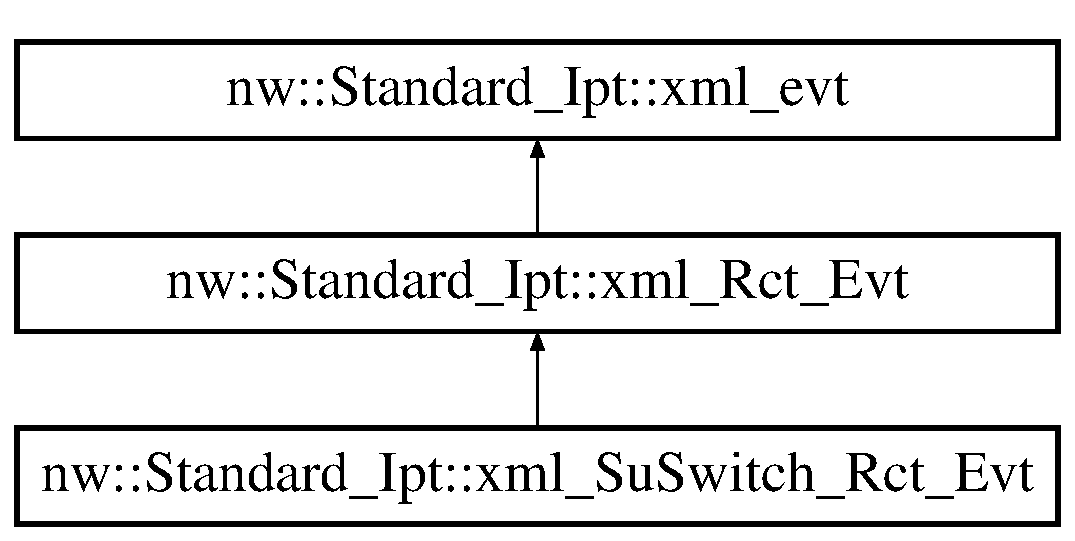
\includegraphics[height=3.000000cm]{d0/d6c/structnw_1_1_standard___ipt_1_1xml___su_switch___rct___evt}
\end{center}
\end{figure}
\subsection*{Public Attributes}
\begin{DoxyCompactItemize}
\item 
long \hyperlink{structnw_1_1_standard___ipt_1_1xml___su_switch___rct___evt_a620a553d11252834116e4ea4af2dc9ce}{xml\+\_\+act\+Su\+\_\+id}
\item 
long \hyperlink{structnw_1_1_standard___ipt_1_1xml___su_switch___rct___evt_a29b04ff37696230c95a126a104ad065b}{xml\+\_\+channel\+\_\+id}
\end{DoxyCompactItemize}


\subsection{Detailed Description}
Structure with attributes of the \hyperlink{classnw_1_1_sub_unit_switch___rct___evt}{Sub\+Unit\+Switch\+\_\+\+Rct\+\_\+\+Evt} class. 

\subsection{Member Data Documentation}
\hypertarget{structnw_1_1_standard___ipt_1_1xml___su_switch___rct___evt_a620a553d11252834116e4ea4af2dc9ce}{\index{nw\+::\+Standard\+\_\+\+Ipt\+::xml\+\_\+\+Su\+Switch\+\_\+\+Rct\+\_\+\+Evt@{nw\+::\+Standard\+\_\+\+Ipt\+::xml\+\_\+\+Su\+Switch\+\_\+\+Rct\+\_\+\+Evt}!xml\+\_\+act\+Su\+\_\+id@{xml\+\_\+act\+Su\+\_\+id}}
\index{xml\+\_\+act\+Su\+\_\+id@{xml\+\_\+act\+Su\+\_\+id}!nw\+::\+Standard\+\_\+\+Ipt\+::xml\+\_\+\+Su\+Switch\+\_\+\+Rct\+\_\+\+Evt@{nw\+::\+Standard\+\_\+\+Ipt\+::xml\+\_\+\+Su\+Switch\+\_\+\+Rct\+\_\+\+Evt}}
\subsubsection[{xml\+\_\+act\+Su\+\_\+id}]{\setlength{\rightskip}{0pt plus 5cm}long nw\+::\+Standard\+\_\+\+Ipt\+::xml\+\_\+\+Su\+Switch\+\_\+\+Rct\+\_\+\+Evt\+::xml\+\_\+act\+Su\+\_\+id}}\label{structnw_1_1_standard___ipt_1_1xml___su_switch___rct___evt_a620a553d11252834116e4ea4af2dc9ce}
\hypertarget{structnw_1_1_standard___ipt_1_1xml___su_switch___rct___evt_a29b04ff37696230c95a126a104ad065b}{\index{nw\+::\+Standard\+\_\+\+Ipt\+::xml\+\_\+\+Su\+Switch\+\_\+\+Rct\+\_\+\+Evt@{nw\+::\+Standard\+\_\+\+Ipt\+::xml\+\_\+\+Su\+Switch\+\_\+\+Rct\+\_\+\+Evt}!xml\+\_\+channel\+\_\+id@{xml\+\_\+channel\+\_\+id}}
\index{xml\+\_\+channel\+\_\+id@{xml\+\_\+channel\+\_\+id}!nw\+::\+Standard\+\_\+\+Ipt\+::xml\+\_\+\+Su\+Switch\+\_\+\+Rct\+\_\+\+Evt@{nw\+::\+Standard\+\_\+\+Ipt\+::xml\+\_\+\+Su\+Switch\+\_\+\+Rct\+\_\+\+Evt}}
\subsubsection[{xml\+\_\+channel\+\_\+id}]{\setlength{\rightskip}{0pt plus 5cm}long nw\+::\+Standard\+\_\+\+Ipt\+::xml\+\_\+\+Su\+Switch\+\_\+\+Rct\+\_\+\+Evt\+::xml\+\_\+channel\+\_\+id}}\label{structnw_1_1_standard___ipt_1_1xml___su_switch___rct___evt_a29b04ff37696230c95a126a104ad065b}


The documentation for this struct was generated from the following file\+:\begin{DoxyCompactItemize}
\item 
Input/\hyperlink{_standard___ipt_8h}{Standard\+\_\+\+Ipt.\+h}\end{DoxyCompactItemize}

\hypertarget{structnw_1_1_standard___ipt_1_1xml__vxl}{\section{nw\+:\+:Standard\+\_\+\+Ipt\+:\+:xml\+\_\+vxl Struct Reference}
\label{structnw_1_1_standard___ipt_1_1xml__vxl}\index{nw\+::\+Standard\+\_\+\+Ipt\+::xml\+\_\+vxl@{nw\+::\+Standard\+\_\+\+Ipt\+::xml\+\_\+vxl}}
}


Structure with attributes of the \hyperlink{classnw_1_1___voxel}{\+\_\+\+Voxel} class.  


\subsection*{Public Attributes}
\begin{DoxyCompactItemize}
\item 
long \hyperlink{structnw_1_1_standard___ipt_1_1xml__vxl_aa3049a5f0e119aded3f128c9451553e1}{xml\+\_\+id}
\item 
vector$<$ long $>$ \hyperlink{structnw_1_1_standard___ipt_1_1xml__vxl_ab4f6ff40cccb2d961d94b356d6ad4eda}{xml\+\_\+init\+\_\+state}
\item 
vector$<$ long $>$ \hyperlink{structnw_1_1_standard___ipt_1_1xml__vxl_abc2d0940cccd69b37fab4029ba180150}{xml\+\_\+vxl\+\_\+neighbours}
\end{DoxyCompactItemize}


\subsection{Detailed Description}
Structure with attributes of the \hyperlink{classnw_1_1___voxel}{\+\_\+\+Voxel} class. 

\subsection{Member Data Documentation}
\hypertarget{structnw_1_1_standard___ipt_1_1xml__vxl_aa3049a5f0e119aded3f128c9451553e1}{\index{nw\+::\+Standard\+\_\+\+Ipt\+::xml\+\_\+vxl@{nw\+::\+Standard\+\_\+\+Ipt\+::xml\+\_\+vxl}!xml\+\_\+id@{xml\+\_\+id}}
\index{xml\+\_\+id@{xml\+\_\+id}!nw\+::\+Standard\+\_\+\+Ipt\+::xml\+\_\+vxl@{nw\+::\+Standard\+\_\+\+Ipt\+::xml\+\_\+vxl}}
\subsubsection[{xml\+\_\+id}]{\setlength{\rightskip}{0pt plus 5cm}long nw\+::\+Standard\+\_\+\+Ipt\+::xml\+\_\+vxl\+::xml\+\_\+id}}\label{structnw_1_1_standard___ipt_1_1xml__vxl_aa3049a5f0e119aded3f128c9451553e1}
\hypertarget{structnw_1_1_standard___ipt_1_1xml__vxl_ab4f6ff40cccb2d961d94b356d6ad4eda}{\index{nw\+::\+Standard\+\_\+\+Ipt\+::xml\+\_\+vxl@{nw\+::\+Standard\+\_\+\+Ipt\+::xml\+\_\+vxl}!xml\+\_\+init\+\_\+state@{xml\+\_\+init\+\_\+state}}
\index{xml\+\_\+init\+\_\+state@{xml\+\_\+init\+\_\+state}!nw\+::\+Standard\+\_\+\+Ipt\+::xml\+\_\+vxl@{nw\+::\+Standard\+\_\+\+Ipt\+::xml\+\_\+vxl}}
\subsubsection[{xml\+\_\+init\+\_\+state}]{\setlength{\rightskip}{0pt plus 5cm}vector$<$long$>$ nw\+::\+Standard\+\_\+\+Ipt\+::xml\+\_\+vxl\+::xml\+\_\+init\+\_\+state}}\label{structnw_1_1_standard___ipt_1_1xml__vxl_ab4f6ff40cccb2d961d94b356d6ad4eda}
\hypertarget{structnw_1_1_standard___ipt_1_1xml__vxl_abc2d0940cccd69b37fab4029ba180150}{\index{nw\+::\+Standard\+\_\+\+Ipt\+::xml\+\_\+vxl@{nw\+::\+Standard\+\_\+\+Ipt\+::xml\+\_\+vxl}!xml\+\_\+vxl\+\_\+neighbours@{xml\+\_\+vxl\+\_\+neighbours}}
\index{xml\+\_\+vxl\+\_\+neighbours@{xml\+\_\+vxl\+\_\+neighbours}!nw\+::\+Standard\+\_\+\+Ipt\+::xml\+\_\+vxl@{nw\+::\+Standard\+\_\+\+Ipt\+::xml\+\_\+vxl}}
\subsubsection[{xml\+\_\+vxl\+\_\+neighbours}]{\setlength{\rightskip}{0pt plus 5cm}vector$<$long$>$ nw\+::\+Standard\+\_\+\+Ipt\+::xml\+\_\+vxl\+::xml\+\_\+vxl\+\_\+neighbours}}\label{structnw_1_1_standard___ipt_1_1xml__vxl_abc2d0940cccd69b37fab4029ba180150}


The documentation for this struct was generated from the following file\+:\begin{DoxyCompactItemize}
\item 
Input/\hyperlink{_standard___ipt_8h}{Standard\+\_\+\+Ipt.\+h}\end{DoxyCompactItemize}

\chapter{File Documentation}
\hypertarget{___event_8h}{\section{Events/\+\_\+\+Event.h File Reference}
\label{___event_8h}\index{Events/\+\_\+\+Event.\+h@{Events/\+\_\+\+Event.\+h}}
}
{\ttfamily \#include $<$vector$>$}\\*
{\ttfamily \#include $<$string$>$}\\*
{\ttfamily \#include $<$cmath$>$}\\*
{\ttfamily \#include $<$iostream$>$}\\*
{\ttfamily \#include \char`\"{}../\+Voxel/\+\_\+\+Voxel.\+h\char`\"{}}\\*
{\ttfamily \#include \char`\"{}../\+Random/\+Uni\+\_\+\+Rnd.\+h\char`\"{}}\\*
\subsection*{Classes}
\begin{DoxyCompactItemize}
\item 
class \hyperlink{classnw_1_1___event}{nw\+::\+\_\+\+Event}
\begin{DoxyCompactList}\small\item\em Abstract base class for system state transitions (events). \end{DoxyCompactList}\item 
struct \hyperlink{structnw_1_1___event_1_1tv__struct}{nw\+::\+\_\+\+Event\+::tv\+\_\+struct}
\begin{DoxyCompactList}\small\item\em tau-\/voxel-\/structure (\hyperlink{structnw_1_1___event_1_1tv__struct}{tv\+\_\+struct}) is a structure that associates a tau value with a \hyperlink{classnw_1_1___voxel}{\+\_\+\+Voxel}. \end{DoxyCompactList}\end{DoxyCompactItemize}
\subsection*{Namespaces}
\begin{DoxyCompactItemize}
\item 
 \hyperlink{namespacenw}{nw}
\end{DoxyCompactItemize}
\subsection*{Typedefs}
\begin{DoxyCompactItemize}
\item 
typedef vector$<$ \+\_\+\+Voxel $\ast$ $>$ \hyperlink{namespacenw_ad7146b8b5a9de9be416847f41135722c}{nw\+::\+Voxel\+Vector}
\begin{DoxyCompactList}\small\item\em typedefs of Vector related structures \end{DoxyCompactList}\item 
typedef Voxel\+Vector\+::iterator \hyperlink{namespacenw_a79f35b5a82b764c7144ecf3074e926c0}{nw\+::\+Voxel\+Iterator}
\begin{DoxyCompactList}\small\item\em typedefs of a \hyperlink{classnw_1_1___voxel}{\+\_\+\+Voxel} vector iterator \end{DoxyCompactList}\end{DoxyCompactItemize}

\hypertarget{_ch_flux___rct___evt_8cpp}{\section{Events/\+Ch\+Flux\+\_\+\+Rct\+\_\+\+Evt.cpp File Reference}
\label{_ch_flux___rct___evt_8cpp}\index{Events/\+Ch\+Flux\+\_\+\+Rct\+\_\+\+Evt.\+cpp@{Events/\+Ch\+Flux\+\_\+\+Rct\+\_\+\+Evt.\+cpp}}
}
{\ttfamily \#include \char`\"{}Ch\+Flux\+\_\+\+Rct\+\_\+\+Evt.\+h\char`\"{}}\\*
{\ttfamily \#include $<$cmath$>$}\\*
\subsection*{Namespaces}
\begin{DoxyCompactItemize}
\item 
 \hyperlink{namespacenw}{nw}
\end{DoxyCompactItemize}

\hypertarget{_ch_flux___rct___evt_8h}{\section{Events/\+Ch\+Flux\+\_\+\+Rct\+\_\+\+Evt.h File Reference}
\label{_ch_flux___rct___evt_8h}\index{Events/\+Ch\+Flux\+\_\+\+Rct\+\_\+\+Evt.\+h@{Events/\+Ch\+Flux\+\_\+\+Rct\+\_\+\+Evt.\+h}}
}
{\ttfamily \#include \char`\"{}Reaction\+\_\+\+Evt.\+h\char`\"{}}\\*
\subsection*{Classes}
\begin{DoxyCompactItemize}
\item 
class \hyperlink{classnw_1_1_ch_flux___rct___evt}{nw\+::\+Ch\+Flux\+\_\+\+Rct\+\_\+\+Evt}
\begin{DoxyCompactList}\small\item\em Channel flux reaction event. \end{DoxyCompactList}\end{DoxyCompactItemize}
\subsection*{Namespaces}
\begin{DoxyCompactItemize}
\item 
 \hyperlink{namespacenw}{nw}
\end{DoxyCompactItemize}

\hypertarget{_diffusion___evt_8cpp}{\section{Events/\+Diffusion\+\_\+\+Evt.cpp File Reference}
\label{_diffusion___evt_8cpp}\index{Events/\+Diffusion\+\_\+\+Evt.\+cpp@{Events/\+Diffusion\+\_\+\+Evt.\+cpp}}
}
{\ttfamily \#include $<$math.\+h$>$}\\*
{\ttfamily \#include $<$iostream$>$}\\*
{\ttfamily \#include $<$exception$>$}\\*
{\ttfamily \#include \char`\"{}Diffusion\+\_\+\+Evt.\+h\char`\"{}}\\*
\subsection*{Namespaces}
\begin{DoxyCompactItemize}
\item 
 \hyperlink{namespacenw}{nw}
\end{DoxyCompactItemize}

\hypertarget{_diffusion___evt_8h}{\section{Events/\+Diffusion\+\_\+\+Evt.h File Reference}
\label{_diffusion___evt_8h}\index{Events/\+Diffusion\+\_\+\+Evt.\+h@{Events/\+Diffusion\+\_\+\+Evt.\+h}}
}
{\ttfamily \#include $<$vector$>$}\\*
{\ttfamily \#include $<$string$>$}\\*
{\ttfamily \#include \char`\"{}../\+Voxel/\+\_\+\+Voxel.\+h\char`\"{}}\\*
{\ttfamily \#include \char`\"{}\+\_\+\+Event.\+h\char`\"{}}\\*
\subsection*{Classes}
\begin{DoxyCompactItemize}
\item 
class \hyperlink{classnw_1_1_diffusion___evt}{nw\+::\+Diffusion\+\_\+\+Evt}
\begin{DoxyCompactList}\small\item\em Realization of diffusion between two voxels. \end{DoxyCompactList}\end{DoxyCompactItemize}
\subsection*{Namespaces}
\begin{DoxyCompactItemize}
\item 
 \hyperlink{namespacenw}{nw}
\end{DoxyCompactItemize}

\hypertarget{_reaction___evt_8cpp}{\section{Events/\+Reaction\+\_\+\+Evt.cpp File Reference}
\label{_reaction___evt_8cpp}\index{Events/\+Reaction\+\_\+\+Evt.\+cpp@{Events/\+Reaction\+\_\+\+Evt.\+cpp}}
}
{\ttfamily \#include $<$math.\+h$>$}\\*
{\ttfamily \#include $<$cmath$>$}\\*
{\ttfamily \#include $<$algorithm$>$}\\*
{\ttfamily \#include $<$iostream$>$}\\*
{\ttfamily \#include $<$exception$>$}\\*
{\ttfamily \#include \char`\"{}../\+Voxel/\+Border\+\_\+\+Vxl.\+h\char`\"{}}\\*
{\ttfamily \#include \char`\"{}Reaction\+\_\+\+Evt.\+h\char`\"{}}\\*
\subsection*{Namespaces}
\begin{DoxyCompactItemize}
\item 
 \hyperlink{namespacenw}{nw}
\end{DoxyCompactItemize}

\hypertarget{_reaction___evt_8h}{\section{Events/\+Reaction\+\_\+\+Evt.h File Reference}
\label{_reaction___evt_8h}\index{Events/\+Reaction\+\_\+\+Evt.\+h@{Events/\+Reaction\+\_\+\+Evt.\+h}}
}
{\ttfamily \#include \char`\"{}\+\_\+\+Event.\+h\char`\"{}}\\*
{\ttfamily \#include $<$vector$>$}\\*
{\ttfamily \#include $<$string$>$}\\*
\subsection*{Classes}
\begin{DoxyCompactItemize}
\item 
class \hyperlink{classnw_1_1_reaction___evt}{nw\+::\+Reaction\+\_\+\+Evt}
\begin{DoxyCompactList}\small\item\em Implementation of the reaction of one ore two molecules. \end{DoxyCompactList}\end{DoxyCompactItemize}
\subsection*{Namespaces}
\begin{DoxyCompactItemize}
\item 
 \hyperlink{namespacenw}{nw}
\end{DoxyCompactItemize}

\hypertarget{_sub_unit_switch___rct___evt_8cpp}{\section{Events/\+Sub\+Unit\+Switch\+\_\+\+Rct\+\_\+\+Evt.cpp File Reference}
\label{_sub_unit_switch___rct___evt_8cpp}\index{Events/\+Sub\+Unit\+Switch\+\_\+\+Rct\+\_\+\+Evt.\+cpp@{Events/\+Sub\+Unit\+Switch\+\_\+\+Rct\+\_\+\+Evt.\+cpp}}
}
{\ttfamily \#include \char`\"{}Sub\+Unit\+Switch\+\_\+\+Rct\+\_\+\+Evt.\+h\char`\"{}}\\*
{\ttfamily \#include $<$math.\+h$>$}\\*
{\ttfamily \#include $<$iostream$>$}\\*

\hypertarget{_sub_unit_switch___rct___evt_8h}{\section{Events/\+Sub\+Unit\+Switch\+\_\+\+Rct\+\_\+\+Evt.h File Reference}
\label{_sub_unit_switch___rct___evt_8h}\index{Events/\+Sub\+Unit\+Switch\+\_\+\+Rct\+\_\+\+Evt.\+h@{Events/\+Sub\+Unit\+Switch\+\_\+\+Rct\+\_\+\+Evt.\+h}}
}
{\ttfamily \#include \char`\"{}Reaction\+\_\+\+Evt.\+h\char`\"{}}\\*
{\ttfamily \#include \char`\"{}../\+Species/\+Channel\+\_\+\+Spc.\+h\char`\"{}}\\*
\subsection*{Classes}
\begin{DoxyCompactItemize}
\item 
class \hyperlink{classnw_1_1_sub_unit_switch___rct___evt}{nw\+::\+Sub\+Unit\+Switch\+\_\+\+Rct\+\_\+\+Evt}
\begin{DoxyCompactList}\small\item\em Subunit switch reaction event. \end{DoxyCompactList}\end{DoxyCompactItemize}
\subsection*{Namespaces}
\begin{DoxyCompactItemize}
\item 
 \hyperlink{namespacenw}{nw}
\end{DoxyCompactItemize}

\hypertarget{___input_8h}{\section{Input/\+\_\+\+Input.h File Reference}
\label{___input_8h}\index{Input/\+\_\+\+Input.\+h@{Input/\+\_\+\+Input.\+h}}
}
{\ttfamily \#include \char`\"{}../\+System/\+\_\+\+System.\+h\char`\"{}}\\*
\subsection*{Classes}
\begin{DoxyCompactItemize}
\item 
class \hyperlink{classnw_1_1___input}{nw\+::\+\_\+\+Input}
\begin{DoxyCompactList}\small\item\em Abstract base class for input procedures. \end{DoxyCompactList}\end{DoxyCompactItemize}
\subsection*{Namespaces}
\begin{DoxyCompactItemize}
\item 
 \hyperlink{namespacenw}{nw}
\end{DoxyCompactItemize}

\hypertarget{_standard___ipt_8cpp}{\section{Input/\+Standard\+\_\+\+Ipt.cpp File Reference}
\label{_standard___ipt_8cpp}\index{Input/\+Standard\+\_\+\+Ipt.\+cpp@{Input/\+Standard\+\_\+\+Ipt.\+cpp}}
}
{\ttfamily \#include \char`\"{}Standard\+\_\+\+Ipt.\+h\char`\"{}}\\*
{\ttfamily \#include $<$iostream$>$}\\*
{\ttfamily \#include $<$math.\+h$>$}\\*
{\ttfamily \#include $<$stdlib.\+h$>$}\\*
{\ttfamily \#include $<$time.\+h$>$}\\*
\subsection*{Namespaces}
\begin{DoxyCompactItemize}
\item 
 \hyperlink{namespacenw}{nw}
\end{DoxyCompactItemize}

\hypertarget{_standard___ipt_8h}{\section{Input/\+Standard\+\_\+\+Ipt.h File Reference}
\label{_standard___ipt_8h}\index{Input/\+Standard\+\_\+\+Ipt.\+h@{Input/\+Standard\+\_\+\+Ipt.\+h}}
}
{\ttfamily \#include \char`\"{}\+\_\+\+Input.\+h\char`\"{}}\\*
{\ttfamily \#include \char`\"{}../\+System/\+Gillespie\+\_\+\+Sys.\+h\char`\"{}}\\*
{\ttfamily \#include \char`\"{}../\+Event\+Header.\+h\char`\"{}}\\*
{\ttfamily \#include \char`\"{}../\+Voxel\+Header.\+h\char`\"{}}\\*
{\ttfamily \#include \char`\"{}../\+Species\+Header.\+h\char`\"{}}\\*
{\ttfamily \#include \char`\"{}../pugi/pugixml.\+hpp\char`\"{}}\\*
\subsection*{Classes}
\begin{DoxyCompactItemize}
\item 
class \hyperlink{classnw_1_1_standard___ipt}{nw\+::\+Standard\+\_\+\+Ipt}
\begin{DoxyCompactList}\small\item\em Input class that parses a .xml files and generates a \hyperlink{classnw_1_1_gillespie___sys}{Gillespie\+\_\+\+Sys}. \end{DoxyCompactList}\item 
struct \hyperlink{structnw_1_1_standard___ipt_1_1xml__evt}{nw\+::\+Standard\+\_\+\+Ipt\+::xml\+\_\+evt}
\begin{DoxyCompactList}\small\item\em Structure with attributes of the \hyperlink{classnw_1_1___event}{\+\_\+\+Event} class. \end{DoxyCompactList}\item 
struct \hyperlink{structnw_1_1_standard___ipt_1_1xml___rct___evt}{nw\+::\+Standard\+\_\+\+Ipt\+::xml\+\_\+\+Rct\+\_\+\+Evt}
\begin{DoxyCompactList}\small\item\em Structure with attributes of the \hyperlink{classnw_1_1_reaction___evt}{Reaction\+\_\+\+Evt} class. \end{DoxyCompactList}\item 
struct \hyperlink{structnw_1_1_standard___ipt_1_1xml___dif___evt}{nw\+::\+Standard\+\_\+\+Ipt\+::xml\+\_\+\+Dif\+\_\+\+Evt}
\begin{DoxyCompactList}\small\item\em Structure with attributes of the \hyperlink{classnw_1_1_diffusion___evt}{Diffusion\+\_\+\+Evt} class. \end{DoxyCompactList}\item 
struct \hyperlink{structnw_1_1_standard___ipt_1_1xml___su_switch___rct___evt}{nw\+::\+Standard\+\_\+\+Ipt\+::xml\+\_\+\+Su\+Switch\+\_\+\+Rct\+\_\+\+Evt}
\begin{DoxyCompactList}\small\item\em Structure with attributes of the \hyperlink{classnw_1_1_sub_unit_switch___rct___evt}{Sub\+Unit\+Switch\+\_\+\+Rct\+\_\+\+Evt} class. \end{DoxyCompactList}\item 
struct \hyperlink{structnw_1_1_standard___ipt_1_1xml___ch_flux___rct___evt}{nw\+::\+Standard\+\_\+\+Ipt\+::xml\+\_\+\+Ch\+Flux\+\_\+\+Rct\+\_\+\+Evt}
\begin{DoxyCompactList}\small\item\em Structure with attributes of the \hyperlink{classnw_1_1_ch_flux___rct___evt}{Ch\+Flux\+\_\+\+Rct\+\_\+\+Evt} class. \end{DoxyCompactList}\item 
struct \hyperlink{structnw_1_1_standard___ipt_1_1xml__vxl}{nw\+::\+Standard\+\_\+\+Ipt\+::xml\+\_\+vxl}
\begin{DoxyCompactList}\small\item\em Structure with attributes of the \hyperlink{classnw_1_1___voxel}{\+\_\+\+Voxel} class. \end{DoxyCompactList}\item 
struct \hyperlink{structnw_1_1_standard___ipt_1_1xml__spc}{nw\+::\+Standard\+\_\+\+Ipt\+::xml\+\_\+spc}
\begin{DoxyCompactList}\small\item\em Structure with attributes of the \hyperlink{classnw_1_1___species}{\+\_\+\+Species} class. \end{DoxyCompactList}\item 
struct \hyperlink{structnw_1_1_standard___ipt_1_1xml___ch___spc}{nw\+::\+Standard\+\_\+\+Ipt\+::xml\+\_\+\+Ch\+\_\+\+Spc}
\begin{DoxyCompactList}\small\item\em Structure with attributes of the \hyperlink{classnw_1_1_channel___spc}{Channel\+\_\+\+Spc} class. \end{DoxyCompactList}\item 
struct \hyperlink{structnw_1_1_standard___ipt_1_1xml__gen__data}{nw\+::\+Standard\+\_\+\+Ipt\+::xml\+\_\+gen\+\_\+data}
\begin{DoxyCompactList}\small\item\em Structure with attributes representing general data necessary for a system. \end{DoxyCompactList}\end{DoxyCompactItemize}
\subsection*{Namespaces}
\begin{DoxyCompactItemize}
\item 
 \hyperlink{namespacenw}{nw}
\end{DoxyCompactItemize}

\hypertarget{mainpage_8dox}{\section{mainpage.\+dox File Reference}
\label{mainpage_8dox}\index{mainpage.\+dox@{mainpage.\+dox}}
}

\hypertarget{___random_8h}{\section{Random/\+\_\+\+Random.h File Reference}
\label{___random_8h}\index{Random/\+\_\+\+Random.\+h@{Random/\+\_\+\+Random.\+h}}
}
\subsection*{Classes}
\begin{DoxyCompactItemize}
\item 
class \hyperlink{classnw_1_1___random}{nw\+::\+\_\+\+Random}
\begin{DoxyCompactList}\small\item\em abstract base class to define an interface for Random Generators \end{DoxyCompactList}\end{DoxyCompactItemize}
\subsection*{Namespaces}
\begin{DoxyCompactItemize}
\item 
 \hyperlink{namespacenw}{nw}
\end{DoxyCompactItemize}

\hypertarget{_uni___rnd_8cpp}{\section{Random/\+Uni\+\_\+\+Rnd.cpp File Reference}
\label{_uni___rnd_8cpp}\index{Random/\+Uni\+\_\+\+Rnd.\+cpp@{Random/\+Uni\+\_\+\+Rnd.\+cpp}}
}
{\ttfamily \#include \char`\"{}Uni\+\_\+\+Rnd.\+h\char`\"{}}\\*
{\ttfamily \#include $<$iostream$>$}\\*
\subsection*{Macros}
\begin{DoxyCompactItemize}
\item 
\#define \hyperlink{_uni___rnd_8cpp_ae4b0efde4fa4613b407716d265d19b0a}{I\+A}~16807
\item 
\#define \hyperlink{_uni___rnd_8cpp_a51c0dfe766601d31e907fceae818a7ca}{I\+M}~2147483647
\item 
\#define \hyperlink{_uni___rnd_8cpp_ad301e6a88b1c01108f4867f2ea6f683c}{A\+M}~(1.\+0/\hyperlink{_uni___rnd_8cpp_a51c0dfe766601d31e907fceae818a7ca}{I\+M})
\item 
\#define \hyperlink{_uni___rnd_8cpp_ab7c5f3342853af6bb48d0ca00b05efbe}{I\+Q}~127773
\item 
\#define \hyperlink{_uni___rnd_8cpp_a68e22635ff207d8ca10459833856bd75}{I\+R}~2836
\item 
\#define \hyperlink{_uni___rnd_8cpp_a0e93cfb2d62849853fd34957ba6e6fdc}{N\+T\+A\+B}~32
\item 
\#define \hyperlink{_uni___rnd_8cpp_a62339d74dd5d9d00480e1a288cf88fe8}{N\+D\+I\+V}~(1+(\hyperlink{_uni___rnd_8cpp_a51c0dfe766601d31e907fceae818a7ca}{I\+M}-\/1)/\hyperlink{_uni___rnd_8cpp_a0e93cfb2d62849853fd34957ba6e6fdc}{N\+T\+A\+B})
\item 
\#define \hyperlink{_uni___rnd_8cpp_a6ebf6899d6c1c8b7b9d09be872c05aae}{E\+P\+S}~1.\+2e-\/7
\item 
\#define \hyperlink{_uni___rnd_8cpp_aa7436c9270ffb06f8c1eae8d2e605cec}{R\+N\+M\+X}~(1.\+0-\/\hyperlink{_uni___rnd_8cpp_a6ebf6899d6c1c8b7b9d09be872c05aae}{E\+P\+S})
\end{DoxyCompactItemize}


\subsection{Macro Definition Documentation}
\hypertarget{_uni___rnd_8cpp_ad301e6a88b1c01108f4867f2ea6f683c}{\index{Uni\+\_\+\+Rnd.\+cpp@{Uni\+\_\+\+Rnd.\+cpp}!A\+M@{A\+M}}
\index{A\+M@{A\+M}!Uni\+\_\+\+Rnd.\+cpp@{Uni\+\_\+\+Rnd.\+cpp}}
\subsubsection[{A\+M}]{\setlength{\rightskip}{0pt plus 5cm}\#define A\+M~(1.\+0/{\bf I\+M})}}\label{_uni___rnd_8cpp_ad301e6a88b1c01108f4867f2ea6f683c}
\hypertarget{_uni___rnd_8cpp_a6ebf6899d6c1c8b7b9d09be872c05aae}{\index{Uni\+\_\+\+Rnd.\+cpp@{Uni\+\_\+\+Rnd.\+cpp}!E\+P\+S@{E\+P\+S}}
\index{E\+P\+S@{E\+P\+S}!Uni\+\_\+\+Rnd.\+cpp@{Uni\+\_\+\+Rnd.\+cpp}}
\subsubsection[{E\+P\+S}]{\setlength{\rightskip}{0pt plus 5cm}\#define E\+P\+S~1.\+2e-\/7}}\label{_uni___rnd_8cpp_a6ebf6899d6c1c8b7b9d09be872c05aae}
\hypertarget{_uni___rnd_8cpp_ae4b0efde4fa4613b407716d265d19b0a}{\index{Uni\+\_\+\+Rnd.\+cpp@{Uni\+\_\+\+Rnd.\+cpp}!I\+A@{I\+A}}
\index{I\+A@{I\+A}!Uni\+\_\+\+Rnd.\+cpp@{Uni\+\_\+\+Rnd.\+cpp}}
\subsubsection[{I\+A}]{\setlength{\rightskip}{0pt plus 5cm}\#define I\+A~16807}}\label{_uni___rnd_8cpp_ae4b0efde4fa4613b407716d265d19b0a}
\hypertarget{_uni___rnd_8cpp_a51c0dfe766601d31e907fceae818a7ca}{\index{Uni\+\_\+\+Rnd.\+cpp@{Uni\+\_\+\+Rnd.\+cpp}!I\+M@{I\+M}}
\index{I\+M@{I\+M}!Uni\+\_\+\+Rnd.\+cpp@{Uni\+\_\+\+Rnd.\+cpp}}
\subsubsection[{I\+M}]{\setlength{\rightskip}{0pt plus 5cm}\#define I\+M~2147483647}}\label{_uni___rnd_8cpp_a51c0dfe766601d31e907fceae818a7ca}
\hypertarget{_uni___rnd_8cpp_ab7c5f3342853af6bb48d0ca00b05efbe}{\index{Uni\+\_\+\+Rnd.\+cpp@{Uni\+\_\+\+Rnd.\+cpp}!I\+Q@{I\+Q}}
\index{I\+Q@{I\+Q}!Uni\+\_\+\+Rnd.\+cpp@{Uni\+\_\+\+Rnd.\+cpp}}
\subsubsection[{I\+Q}]{\setlength{\rightskip}{0pt plus 5cm}\#define I\+Q~127773}}\label{_uni___rnd_8cpp_ab7c5f3342853af6bb48d0ca00b05efbe}
\hypertarget{_uni___rnd_8cpp_a68e22635ff207d8ca10459833856bd75}{\index{Uni\+\_\+\+Rnd.\+cpp@{Uni\+\_\+\+Rnd.\+cpp}!I\+R@{I\+R}}
\index{I\+R@{I\+R}!Uni\+\_\+\+Rnd.\+cpp@{Uni\+\_\+\+Rnd.\+cpp}}
\subsubsection[{I\+R}]{\setlength{\rightskip}{0pt plus 5cm}\#define I\+R~2836}}\label{_uni___rnd_8cpp_a68e22635ff207d8ca10459833856bd75}
\hypertarget{_uni___rnd_8cpp_a62339d74dd5d9d00480e1a288cf88fe8}{\index{Uni\+\_\+\+Rnd.\+cpp@{Uni\+\_\+\+Rnd.\+cpp}!N\+D\+I\+V@{N\+D\+I\+V}}
\index{N\+D\+I\+V@{N\+D\+I\+V}!Uni\+\_\+\+Rnd.\+cpp@{Uni\+\_\+\+Rnd.\+cpp}}
\subsubsection[{N\+D\+I\+V}]{\setlength{\rightskip}{0pt plus 5cm}\#define N\+D\+I\+V~(1+({\bf I\+M}-\/1)/{\bf N\+T\+A\+B})}}\label{_uni___rnd_8cpp_a62339d74dd5d9d00480e1a288cf88fe8}
\hypertarget{_uni___rnd_8cpp_a0e93cfb2d62849853fd34957ba6e6fdc}{\index{Uni\+\_\+\+Rnd.\+cpp@{Uni\+\_\+\+Rnd.\+cpp}!N\+T\+A\+B@{N\+T\+A\+B}}
\index{N\+T\+A\+B@{N\+T\+A\+B}!Uni\+\_\+\+Rnd.\+cpp@{Uni\+\_\+\+Rnd.\+cpp}}
\subsubsection[{N\+T\+A\+B}]{\setlength{\rightskip}{0pt plus 5cm}\#define N\+T\+A\+B~32}}\label{_uni___rnd_8cpp_a0e93cfb2d62849853fd34957ba6e6fdc}
\hypertarget{_uni___rnd_8cpp_aa7436c9270ffb06f8c1eae8d2e605cec}{\index{Uni\+\_\+\+Rnd.\+cpp@{Uni\+\_\+\+Rnd.\+cpp}!R\+N\+M\+X@{R\+N\+M\+X}}
\index{R\+N\+M\+X@{R\+N\+M\+X}!Uni\+\_\+\+Rnd.\+cpp@{Uni\+\_\+\+Rnd.\+cpp}}
\subsubsection[{R\+N\+M\+X}]{\setlength{\rightskip}{0pt plus 5cm}\#define R\+N\+M\+X~(1.\+0-\/{\bf E\+P\+S})}}\label{_uni___rnd_8cpp_aa7436c9270ffb06f8c1eae8d2e605cec}

\hypertarget{_uni___rnd_8h}{\section{Random/\+Uni\+\_\+\+Rnd.h File Reference}
\label{_uni___rnd_8h}\index{Random/\+Uni\+\_\+\+Rnd.\+h@{Random/\+Uni\+\_\+\+Rnd.\+h}}
}
{\ttfamily \#include \char`\"{}\+\_\+\+Random.\+h\char`\"{}}\\*
{\ttfamily \#include $<$time.\+h$>$}\\*
\subsection*{Classes}
\begin{DoxyCompactItemize}
\item 
class \hyperlink{classnw_1_1_uni___rnd}{nw\+::\+Uni\+\_\+\+Rnd}
\begin{DoxyCompactList}\small\item\em \char`\"{}\+Minimal\char`\"{} random number generator of Park and Miller \end{DoxyCompactList}\end{DoxyCompactItemize}
\subsection*{Namespaces}
\begin{DoxyCompactItemize}
\item 
 \hyperlink{namespacenw}{nw}
\end{DoxyCompactItemize}

\hypertarget{___species_8h}{\section{Species/\+\_\+\+Species.h File Reference}
\label{___species_8h}\index{Species/\+\_\+\+Species.\+h@{Species/\+\_\+\+Species.\+h}}
}
{\ttfamily \#include $<$string$>$}\\*
\subsection*{Classes}
\begin{DoxyCompactItemize}
\item 
class \hyperlink{classnw_1_1___species}{nw\+::\+\_\+\+Species}
\begin{DoxyCompactList}\small\item\em Abstract base class for the molecular species of a system. \end{DoxyCompactList}\end{DoxyCompactItemize}
\subsection*{Namespaces}
\begin{DoxyCompactItemize}
\item 
 \hyperlink{namespacenw}{nw}
\end{DoxyCompactItemize}
\subsection*{Variables}
\begin{DoxyCompactItemize}
\item 
static const double \hyperlink{namespacenw_ad890cfa7dd9eaf8d5b6754723e516c4a}{nw\+::\+N\+\_\+\+A\+V\+O} = 6.\+022e23
\end{DoxyCompactItemize}

\hypertarget{_channel___spc_8cpp}{\section{Species/\+Channel\+\_\+\+Spc.cpp File Reference}
\label{_channel___spc_8cpp}\index{Species/\+Channel\+\_\+\+Spc.\+cpp@{Species/\+Channel\+\_\+\+Spc.\+cpp}}
}
{\ttfamily \#include \char`\"{}Channel\+\_\+\+Spc.\+h\char`\"{}}\\*
{\ttfamily \#include $<$iostream$>$}\\*
\subsection*{Namespaces}
\begin{DoxyCompactItemize}
\item 
 \hyperlink{namespacenw}{nw}
\end{DoxyCompactItemize}

\hypertarget{_channel___spc_8h}{\section{Species/\+Channel\+\_\+\+Spc.h File Reference}
\label{_channel___spc_8h}\index{Species/\+Channel\+\_\+\+Spc.\+h@{Species/\+Channel\+\_\+\+Spc.\+h}}
}
{\ttfamily \#include \char`\"{}\+\_\+\+Species.\+h\char`\"{}}\\*
{\ttfamily \#include $<$iostream$>$}\\*
{\ttfamily \#include $<$vector$>$}\\*
\subsection*{Classes}
\begin{DoxyCompactItemize}
\item 
class \hyperlink{classnw_1_1_channel___spc}{nw\+::\+Channel\+\_\+\+Spc}
\begin{DoxyCompactList}\small\item\em Realization of channel proteins comprised of a fixed number of subunits that open whenever a predefined number of those subunits are in an active state. \end{DoxyCompactList}\end{DoxyCompactItemize}
\subsection*{Namespaces}
\begin{DoxyCompactItemize}
\item 
 \hyperlink{namespacenw}{nw}
\end{DoxyCompactItemize}

\hypertarget{_standard___spc_8h}{\section{Species/\+Standard\+\_\+\+Spc.h File Reference}
\label{_standard___spc_8h}\index{Species/\+Standard\+\_\+\+Spc.\+h@{Species/\+Standard\+\_\+\+Spc.\+h}}
}
{\ttfamily \#include $<$iostream$>$}\\*
{\ttfamily \#include \char`\"{}\+\_\+\+Species.\+h\char`\"{}}\\*
\subsection*{Classes}
\begin{DoxyCompactItemize}
\item 
class \hyperlink{classnw_1_1_standard___spc}{nw\+::\+Standard\+\_\+\+Spc}
\begin{DoxyCompactList}\small\item\em Basic implementation of a standard moecular species. \end{DoxyCompactList}\end{DoxyCompactItemize}
\subsection*{Namespaces}
\begin{DoxyCompactItemize}
\item 
 \hyperlink{namespacenw}{nw}
\end{DoxyCompactItemize}

\hypertarget{___system_8h}{\section{System/\+\_\+\+System.h File Reference}
\label{___system_8h}\index{System/\+\_\+\+System.\+h@{System/\+\_\+\+System.\+h}}
}
\subsection*{Classes}
\begin{DoxyCompactItemize}
\item 
class \hyperlink{classnw_1_1___system}{nw\+::\+\_\+\+System}
\begin{DoxyCompactList}\small\item\em Abstract base class for the implementation of simulation algorithms. \end{DoxyCompactList}\end{DoxyCompactItemize}
\subsection*{Namespaces}
\begin{DoxyCompactItemize}
\item 
 \hyperlink{namespacenw}{nw}
\end{DoxyCompactItemize}

\hypertarget{_gillespie___sys_8cpp}{\section{System/\+Gillespie\+\_\+\+Sys.cpp File Reference}
\label{_gillespie___sys_8cpp}\index{System/\+Gillespie\+\_\+\+Sys.\+cpp@{System/\+Gillespie\+\_\+\+Sys.\+cpp}}
}
{\ttfamily \#include $<$iostream$>$}\\*
{\ttfamily \#include $<$algorithm$>$}\\*
{\ttfamily \#include $<$exception$>$}\\*
{\ttfamily \#include $<$cmath$>$}\\*
{\ttfamily \#include $<$ios$>$}\\*
{\ttfamily \#include $<$iomanip$>$}\\*
{\ttfamily \#include \char`\"{}Gillespie\+\_\+\+Sys.\+h\char`\"{}}\\*
\subsection*{Namespaces}
\begin{DoxyCompactItemize}
\item 
 \hyperlink{namespacenw}{nw}
\end{DoxyCompactItemize}

\hypertarget{_gillespie___sys_8h}{\section{System/\+Gillespie\+\_\+\+Sys.h File Reference}
\label{_gillespie___sys_8h}\index{System/\+Gillespie\+\_\+\+Sys.\+h@{System/\+Gillespie\+\_\+\+Sys.\+h}}
}
{\ttfamily \#include $<$vector$>$}\\*
{\ttfamily \#include $<$fstream$>$}\\*
{\ttfamily \#include $<$sstream$>$}\\*
{\ttfamily \#include \char`\"{}\+\_\+\+System.\+h\char`\"{}}\\*
{\ttfamily \#include \char`\"{}../\+Events/\+\_\+\+Event.\+h\char`\"{}}\\*
{\ttfamily \#include \char`\"{}../\+Voxel/\+\_\+\+Voxel.\+h\char`\"{}}\\*
\subsection*{Classes}
\begin{DoxyCompactItemize}
\item 
class \hyperlink{classnw_1_1_gillespie___sys}{nw\+::\+Gillespie\+\_\+\+Sys}
\begin{DoxyCompactList}\small\item\em Coordinates the stochastic simulation algorithm. \end{DoxyCompactList}\end{DoxyCompactItemize}
\subsection*{Namespaces}
\begin{DoxyCompactItemize}
\item 
 \hyperlink{namespacenw}{nw}
\end{DoxyCompactItemize}
\subsection*{Typedefs}
\begin{DoxyCompactItemize}
\item 
typedef vector$<$ \+\_\+\+Event $\ast$ $>$ \hyperlink{namespacenw_a0d9ea27d7802637354c7892806eac1fc}{nw\+::\+Event\+Vector}
\begin{DoxyCompactList}\small\item\em typedefs of a \hyperlink{classnw_1_1___event}{\+\_\+\+Event} reference vector \end{DoxyCompactList}\item 
typedef Event\+Vector\+::iterator \hyperlink{namespacenw_a543a4f72e609ca94582c1c7c10303e0b}{nw\+::\+Event\+Iterator}
\begin{DoxyCompactList}\small\item\em typedefs of a \hyperlink{classnw_1_1___event}{\+\_\+\+Event} vector iterator \end{DoxyCompactList}\end{DoxyCompactItemize}
\subsection*{Variables}
\begin{DoxyCompactItemize}
\item 
static const string \hyperlink{namespacenw_a7d9622d3fd42f8d91bb8b8a79688518d}{nw\+::\+N\+E\+G\+A\+T\+I\+V\+E\+T\+A\+U\+M\+S\+G} = \char`\"{}N\+E\+G\+A\+T\+I\+V\+E T\+A\+U E\+R\+R\+O\+R L\+A\+S\+T E\+V\+E\+N\+T \char`\"{}
\begin{DoxyCompactList}\small\item\em Error message that is thrown, whenever the smallest tau value becomes negative. \end{DoxyCompactList}\end{DoxyCompactItemize}

\hypertarget{___voxel_8h}{\section{Voxel/\+\_\+\+Voxel.h File Reference}
\label{___voxel_8h}\index{Voxel/\+\_\+\+Voxel.\+h@{Voxel/\+\_\+\+Voxel.\+h}}
}
{\ttfamily \#include \char`\"{}../\+Species/\+\_\+\+Species.\+h\char`\"{}}\\*
{\ttfamily \#include $<$iostream$>$}\\*
{\ttfamily \#include $<$math.\+h$>$}\\*
\subsection*{Classes}
\begin{DoxyCompactItemize}
\item 
class \hyperlink{classnw_1_1___voxel}{nw\+::\+\_\+\+Voxel}
\begin{DoxyCompactList}\small\item\em Abstract base class for voxel (discrete building blocks of the simulation volume) \end{DoxyCompactList}\end{DoxyCompactItemize}
\subsection*{Namespaces}
\begin{DoxyCompactItemize}
\item 
 \hyperlink{namespacenw}{nw}
\end{DoxyCompactItemize}
\subsection*{Typedefs}
\begin{DoxyCompactItemize}
\item 
typedef vector$<$ \+\_\+\+Species $\ast$ $>$ \hyperlink{namespacenw_a68aa8285591d78ebfc793c531bd43a23}{nw\+::\+Species\+Vector}
\begin{DoxyCompactList}\small\item\em typedefs of Species related structures \end{DoxyCompactList}\item 
typedef Species\+Vector\+::iterator \hyperlink{namespacenw_a28941aaaa0562445c168a620b63547d2}{nw\+::\+Species\+Iterator}
\end{DoxyCompactItemize}

\hypertarget{_border___vxl_8cpp}{\section{Voxel/\+Border\+\_\+\+Vxl.cpp File Reference}
\label{_border___vxl_8cpp}\index{Voxel/\+Border\+\_\+\+Vxl.\+cpp@{Voxel/\+Border\+\_\+\+Vxl.\+cpp}}
}
{\ttfamily \#include \char`\"{}Border\+\_\+\+Vxl.\+h\char`\"{}}\\*
{\ttfamily \#include $<$iostream$>$}\\*
{\ttfamily \#include $<$math.\+h$>$}\\*
\subsection*{Namespaces}
\begin{DoxyCompactItemize}
\item 
 \hyperlink{namespacenw}{nw}
\end{DoxyCompactItemize}

\hypertarget{_border___vxl_8h}{\section{Voxel/\+Border\+\_\+\+Vxl.h File Reference}
\label{_border___vxl_8h}\index{Voxel/\+Border\+\_\+\+Vxl.\+h@{Voxel/\+Border\+\_\+\+Vxl.\+h}}
}
{\ttfamily \#include $<$vector$>$}\\*
{\ttfamily \#include \char`\"{}\+\_\+\+Voxel.\+h\char`\"{}}\\*
{\ttfamily \#include \char`\"{}../\+Species/\+\_\+\+Species.\+h\char`\"{}}\\*
\subsection*{Classes}
\begin{DoxyCompactItemize}
\item 
class \hyperlink{classnw_1_1_border___vxl}{nw\+::\+Border\+\_\+\+Vxl}
\begin{DoxyCompactList}\small\item\em Specialized \hyperlink{classnw_1_1___voxel}{\+\_\+\+Voxel} that can be used to define a system with equilibrium as boundary condition. \end{DoxyCompactList}\end{DoxyCompactItemize}
\subsection*{Namespaces}
\begin{DoxyCompactItemize}
\item 
 \hyperlink{namespacenw}{nw}
\end{DoxyCompactItemize}

\hypertarget{_standard___vxl_8cpp}{\section{Voxel/\+Standard\+\_\+\+Vxl.cpp File Reference}
\label{_standard___vxl_8cpp}\index{Voxel/\+Standard\+\_\+\+Vxl.\+cpp@{Voxel/\+Standard\+\_\+\+Vxl.\+cpp}}
}
{\ttfamily \#include \char`\"{}Standard\+\_\+\+Vxl.\+h\char`\"{}}\\*
{\ttfamily \#include $<$iostream$>$}\\*
{\ttfamily \#include $<$math.\+h$>$}\\*
\subsection*{Namespaces}
\begin{DoxyCompactItemize}
\item 
 \hyperlink{namespacenw}{nw}
\end{DoxyCompactItemize}

\hypertarget{_standard___vxl_8h}{\section{Voxel/\+Standard\+\_\+\+Vxl.h File Reference}
\label{_standard___vxl_8h}\index{Voxel/\+Standard\+\_\+\+Vxl.\+h@{Voxel/\+Standard\+\_\+\+Vxl.\+h}}
}
{\ttfamily \#include $<$vector$>$}\\*
{\ttfamily \#include \char`\"{}\+\_\+\+Voxel.\+h\char`\"{}}\\*
{\ttfamily \#include \char`\"{}../\+Species/\+\_\+\+Species.\+h\char`\"{}}\\*
\subsection*{Classes}
\begin{DoxyCompactItemize}
\item 
class \hyperlink{classnw_1_1_standard___vxl}{nw\+::\+Standard\+\_\+\+Vxl}
\begin{DoxyCompactList}\small\item\em Standard voxel implementation. \end{DoxyCompactList}\end{DoxyCompactItemize}
\subsection*{Namespaces}
\begin{DoxyCompactItemize}
\item 
 \hyperlink{namespacenw}{nw}
\end{DoxyCompactItemize}

%--- End generated contents ---

% Index
\newpage
\phantomsection
\addcontentsline{toc}{chapter}{Index}
\printindex

\end{document}
